%%==========================================================================
\section{Experiments}
\label{sec:experiments}

We have used synthetically generated random data as well as real images to evaluate our proposed method, and to provide comparisons to other state-of-art algorithms. The first experiment uses artificial data, while the other three use real image data for three classical correspondence problems: image matching under affine transformation, image matching on deformable surfaces, and image matching under projective transformations.

We used third-order feature matching for the artificial data experiment, for deformable surface matching and for projective image matching. Our fourth-order feature matching approach was applied to affine image matching.

We chose as a basis for comparison bipartite graph matching~\cite{Belongie02} (a first-order method), the spectral method~\cite{Cour06} (a pairwise method), a third-order tensor method~\cite{Duchenne_etal09} and the hyper graph matching method~\cite{Zass08}, using the authors' code in each case.
To enable direct comparison, the third-order tensor method~\cite{Duchenne_etal09}, the hyper graph matching method~\cite{Zass08} and our method used the same potential.

%-------------------------------------------------------------------------
\subsection{Artificial data}
\label{subsec:artificialdata}

First we used artificial data to verify the performance of our method quantitatively, using a rotation test, a rescaling test, a distortion test and an outlier test.

For the first three tests, we generated 50 random points in the 2D plane for $P_1$, then $P_2$ was obtained by the following formula:
\begin{flalign*}
\begin{split}
&\text{Rotation test: }\\
&\quad{   }\;P_2 =R_\alpha  \cdot S_\delta\cdot P_1 + N(0,0.05),\ \alpha \in\{0,7\pi/4\}\;\text{ step }\pi/4, \forall S_\delta\in(0.5,1.5)\\
&\text{Scaling test: }\\
&\quad{   }\;P_2 =R_{\delta'}  \cdot S\cdot P_1 + N(0,0.05),\ S\in \{1,2,4,6,8\},
 \forall \delta'\in (-10^\circ,10^\circ)\\
&\text{Distortion test: }\\
&\quad{   }\;P_2  =R_{\delta'} \cdot S_\delta\cdot P_1 + N(0,\sigma),\ \sigma\in [0,1],\; \forall \delta'\in (-10^\circ,10^\circ),\;\forall S_\delta\in(0.5,1.5)\\
\end{split}&
\end{flalign*}
where $S_\delta$ and $R_{\delta'}$ are small random disturbances of scale and rotation angle in the ranges $(0.5,1.5)$ and $(-10^\circ,10^\circ)$ respectively. $N$, $S$ and $\sigma$ stand for Gaussian noise, the scaling factor and noise variance separately. In the rotation test, all points in $P_1$ were rotated through the same angle $\alpha$ around the origin. In the scaling test, all points in $P_2$ were scaled by the same factor $S$. $P_2$ in the distortion test was generated by perturbing the positions of all points in $P_1$ using Gaussian noise $N$.

For the outlier test, we generated 20 random points as $P_1$, and the point set $P_2$ was obtained by adding random numbers of outliers (from $0-60$ step $10$, $60-100$ step $5$) to $P_1$, then small random changes of scale and rotation were added, as well as Gaussian noise ($\sigma=0.05$).

\begin{figure*}[!t]
%\vspace{-4mm}
%\hspace{-8ex}
\setlength{\abovecaptionskip}{1mm}
\setlength{\belowcaptionskip}{0mm}
\centering
\setlength\subfigcapskip{-4mm}
%\hspace{-12ex}
        %----------------------------
        \hspace{-16mm}
        \begin{minipage}[b]{0.4\textwidth}
            \subfigure[]{
            \label{fig:subfig:rtest}
            \centering
            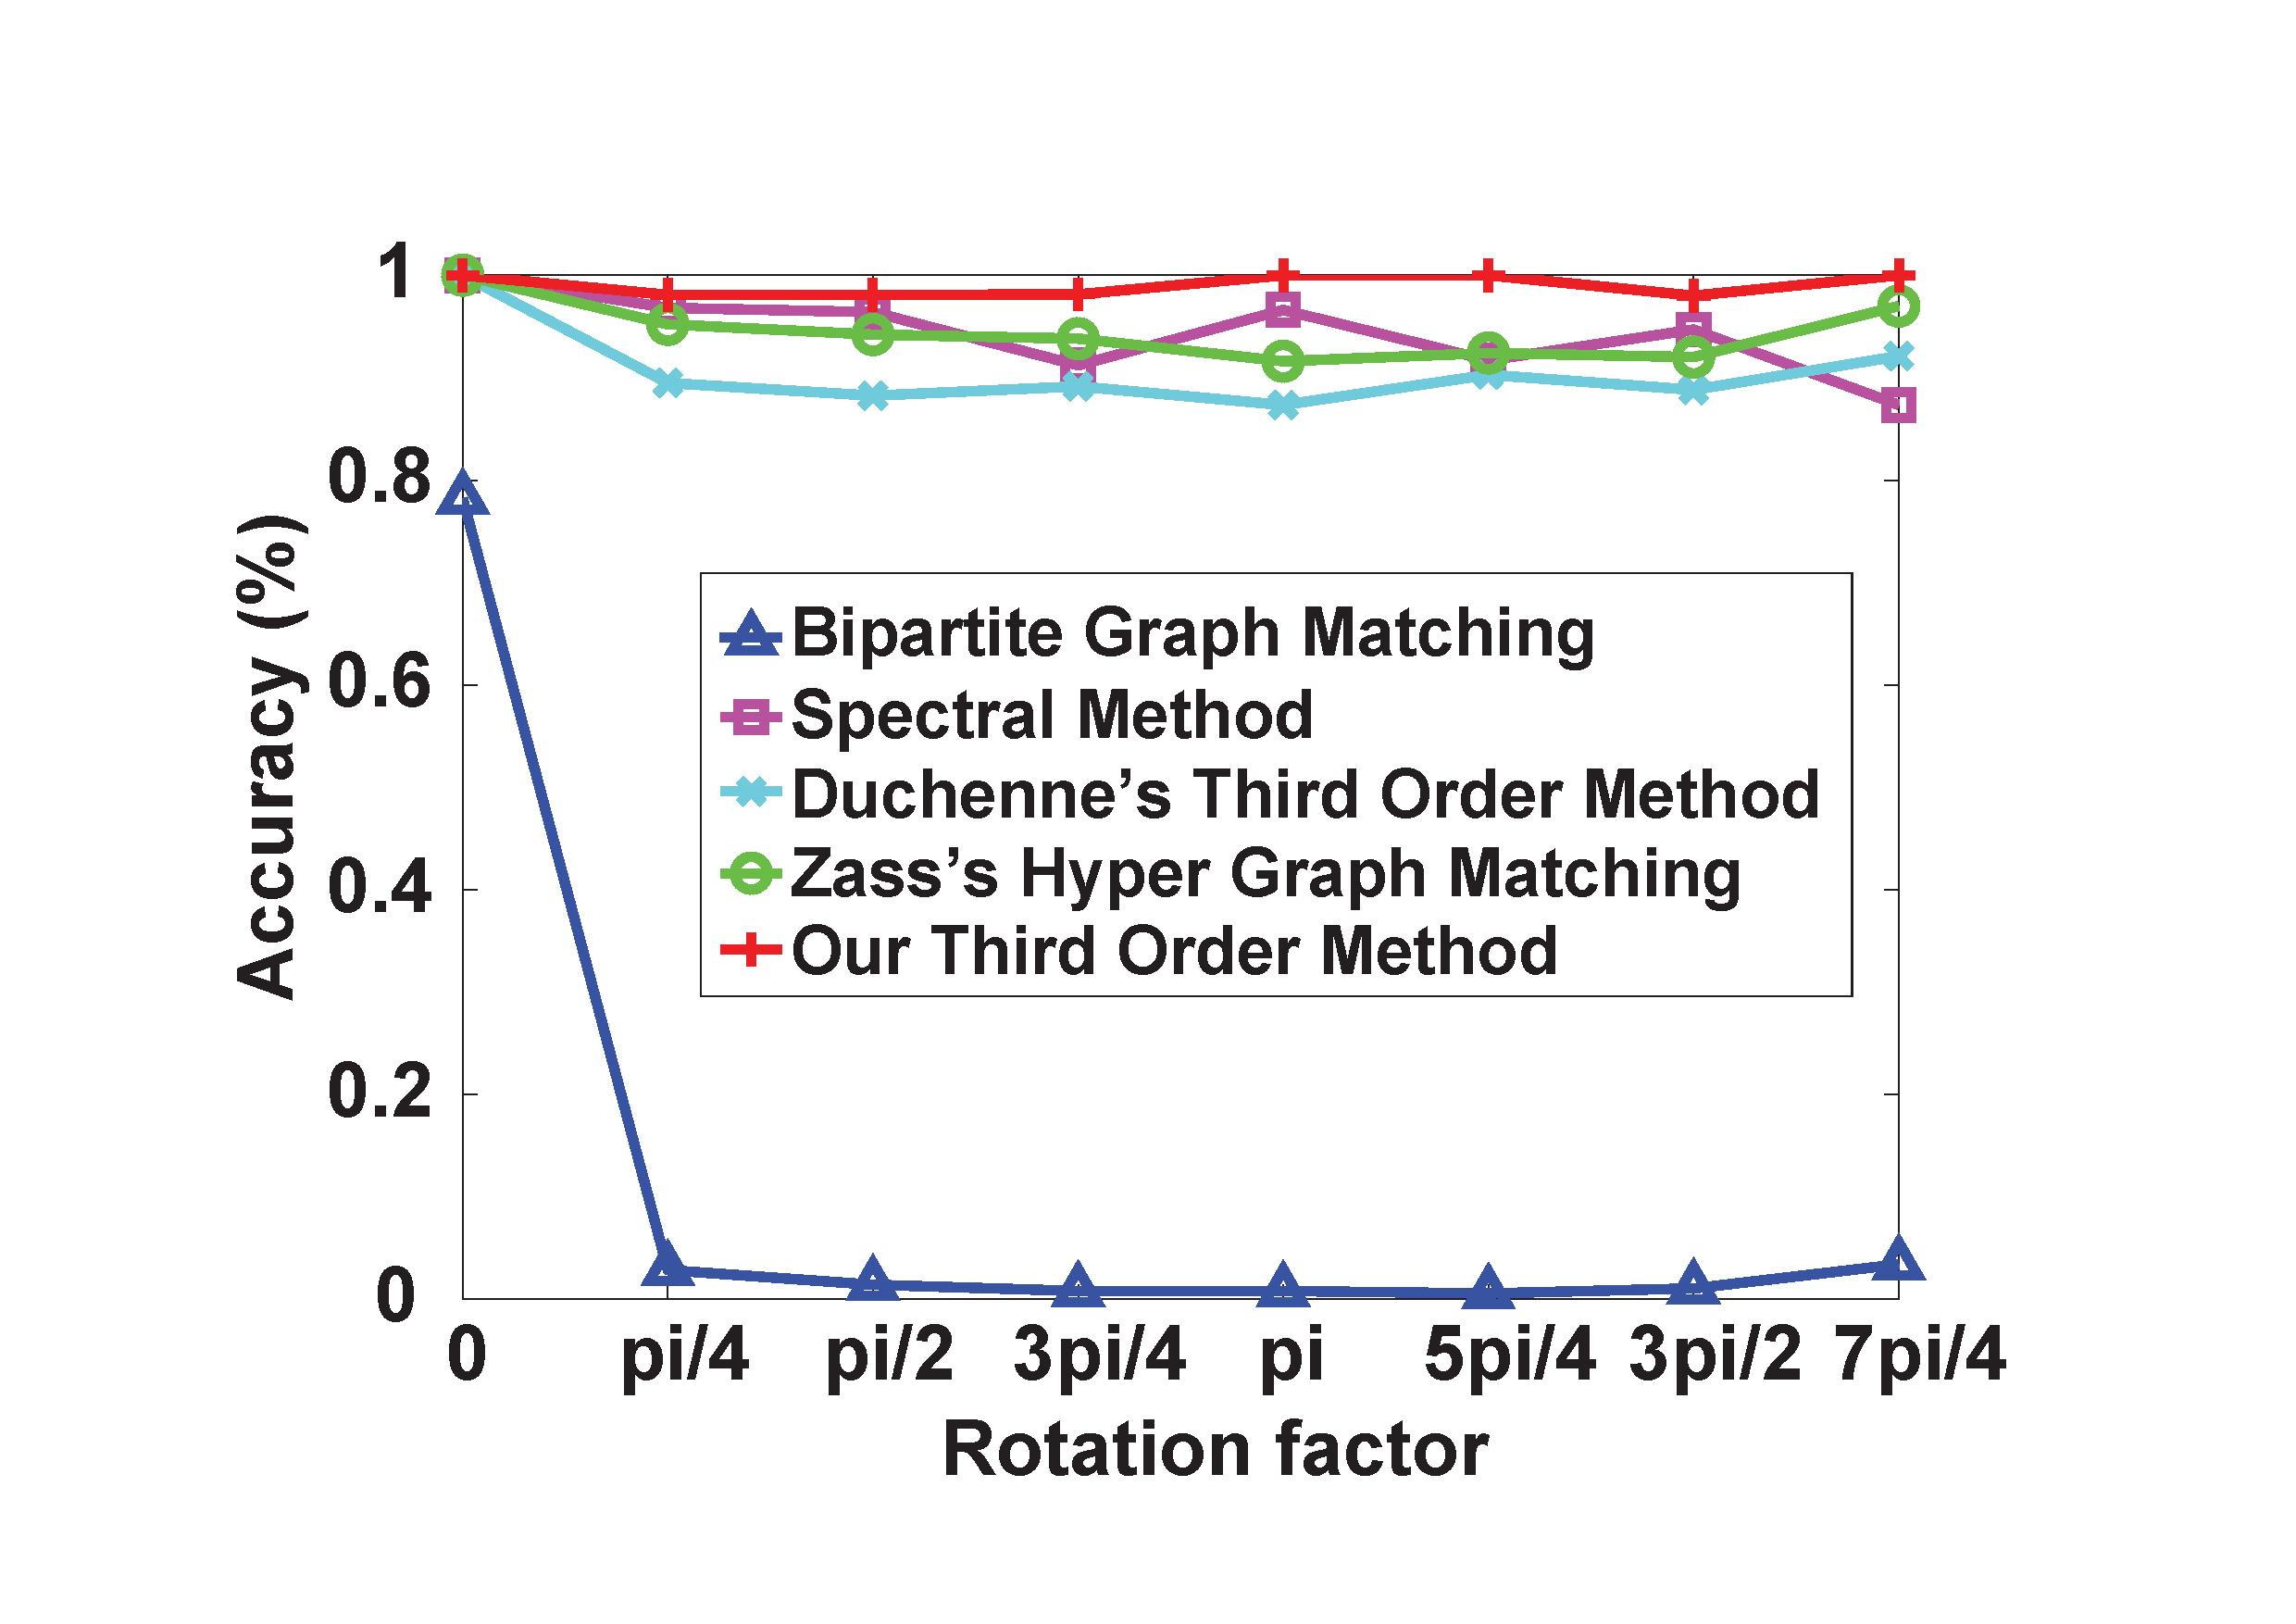
\includegraphics[width=65mm]{rtest_embedded2.pdf}}%
        \end{minipage}%
        \hspace{16mm}%
        %\addtocounter{subfigure}{-1}
        %----------------------------
        \begin{minipage}[b]{0.4\textwidth}
            \subfigure[]{
            \label{fig:subfig:stest}
            \centering
            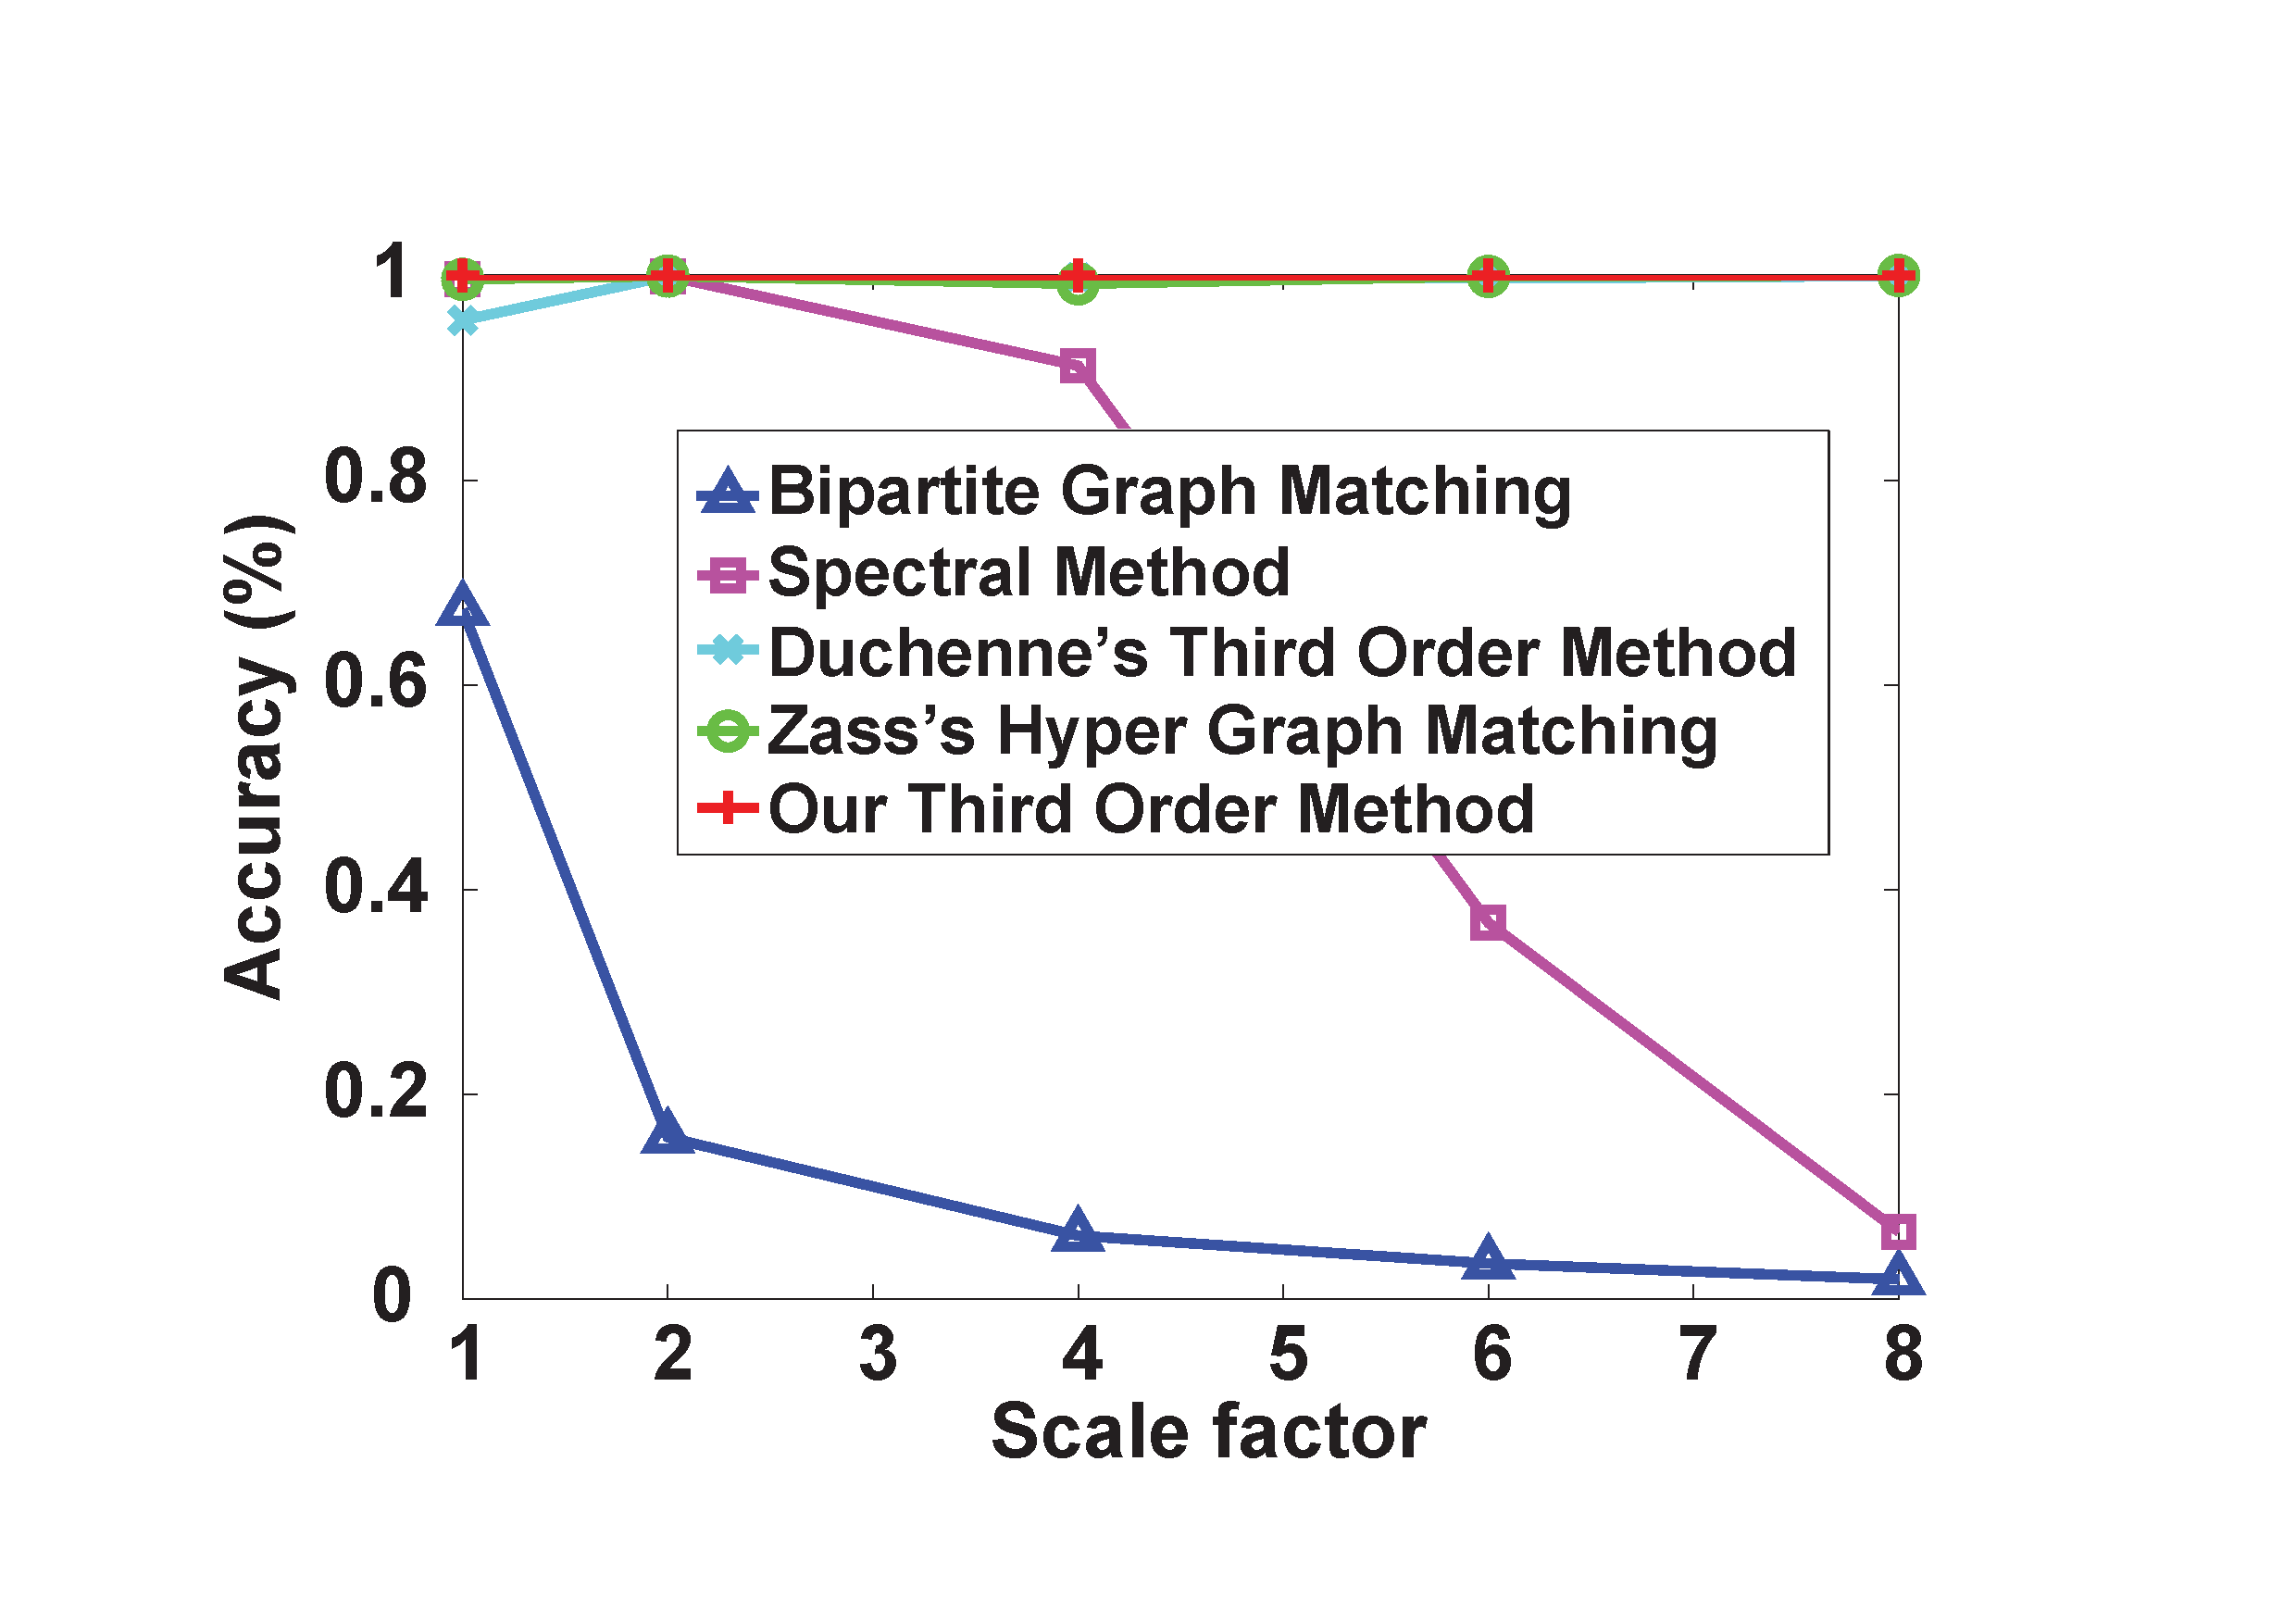
\includegraphics[width=65mm]{stest_embedded2.pdf}}%
        \end{minipage}\\%
        %\vspace{-2mm}%
        %\hspace{14mm}%
        %\addtocounter{subfigure}{-1}
        %----------------------------
        \hspace{-16mm}
        \begin{minipage}[b]{0.4\textwidth}
            \subfigure[]{
            \label{fig:subfig:dtest}
            \centering
            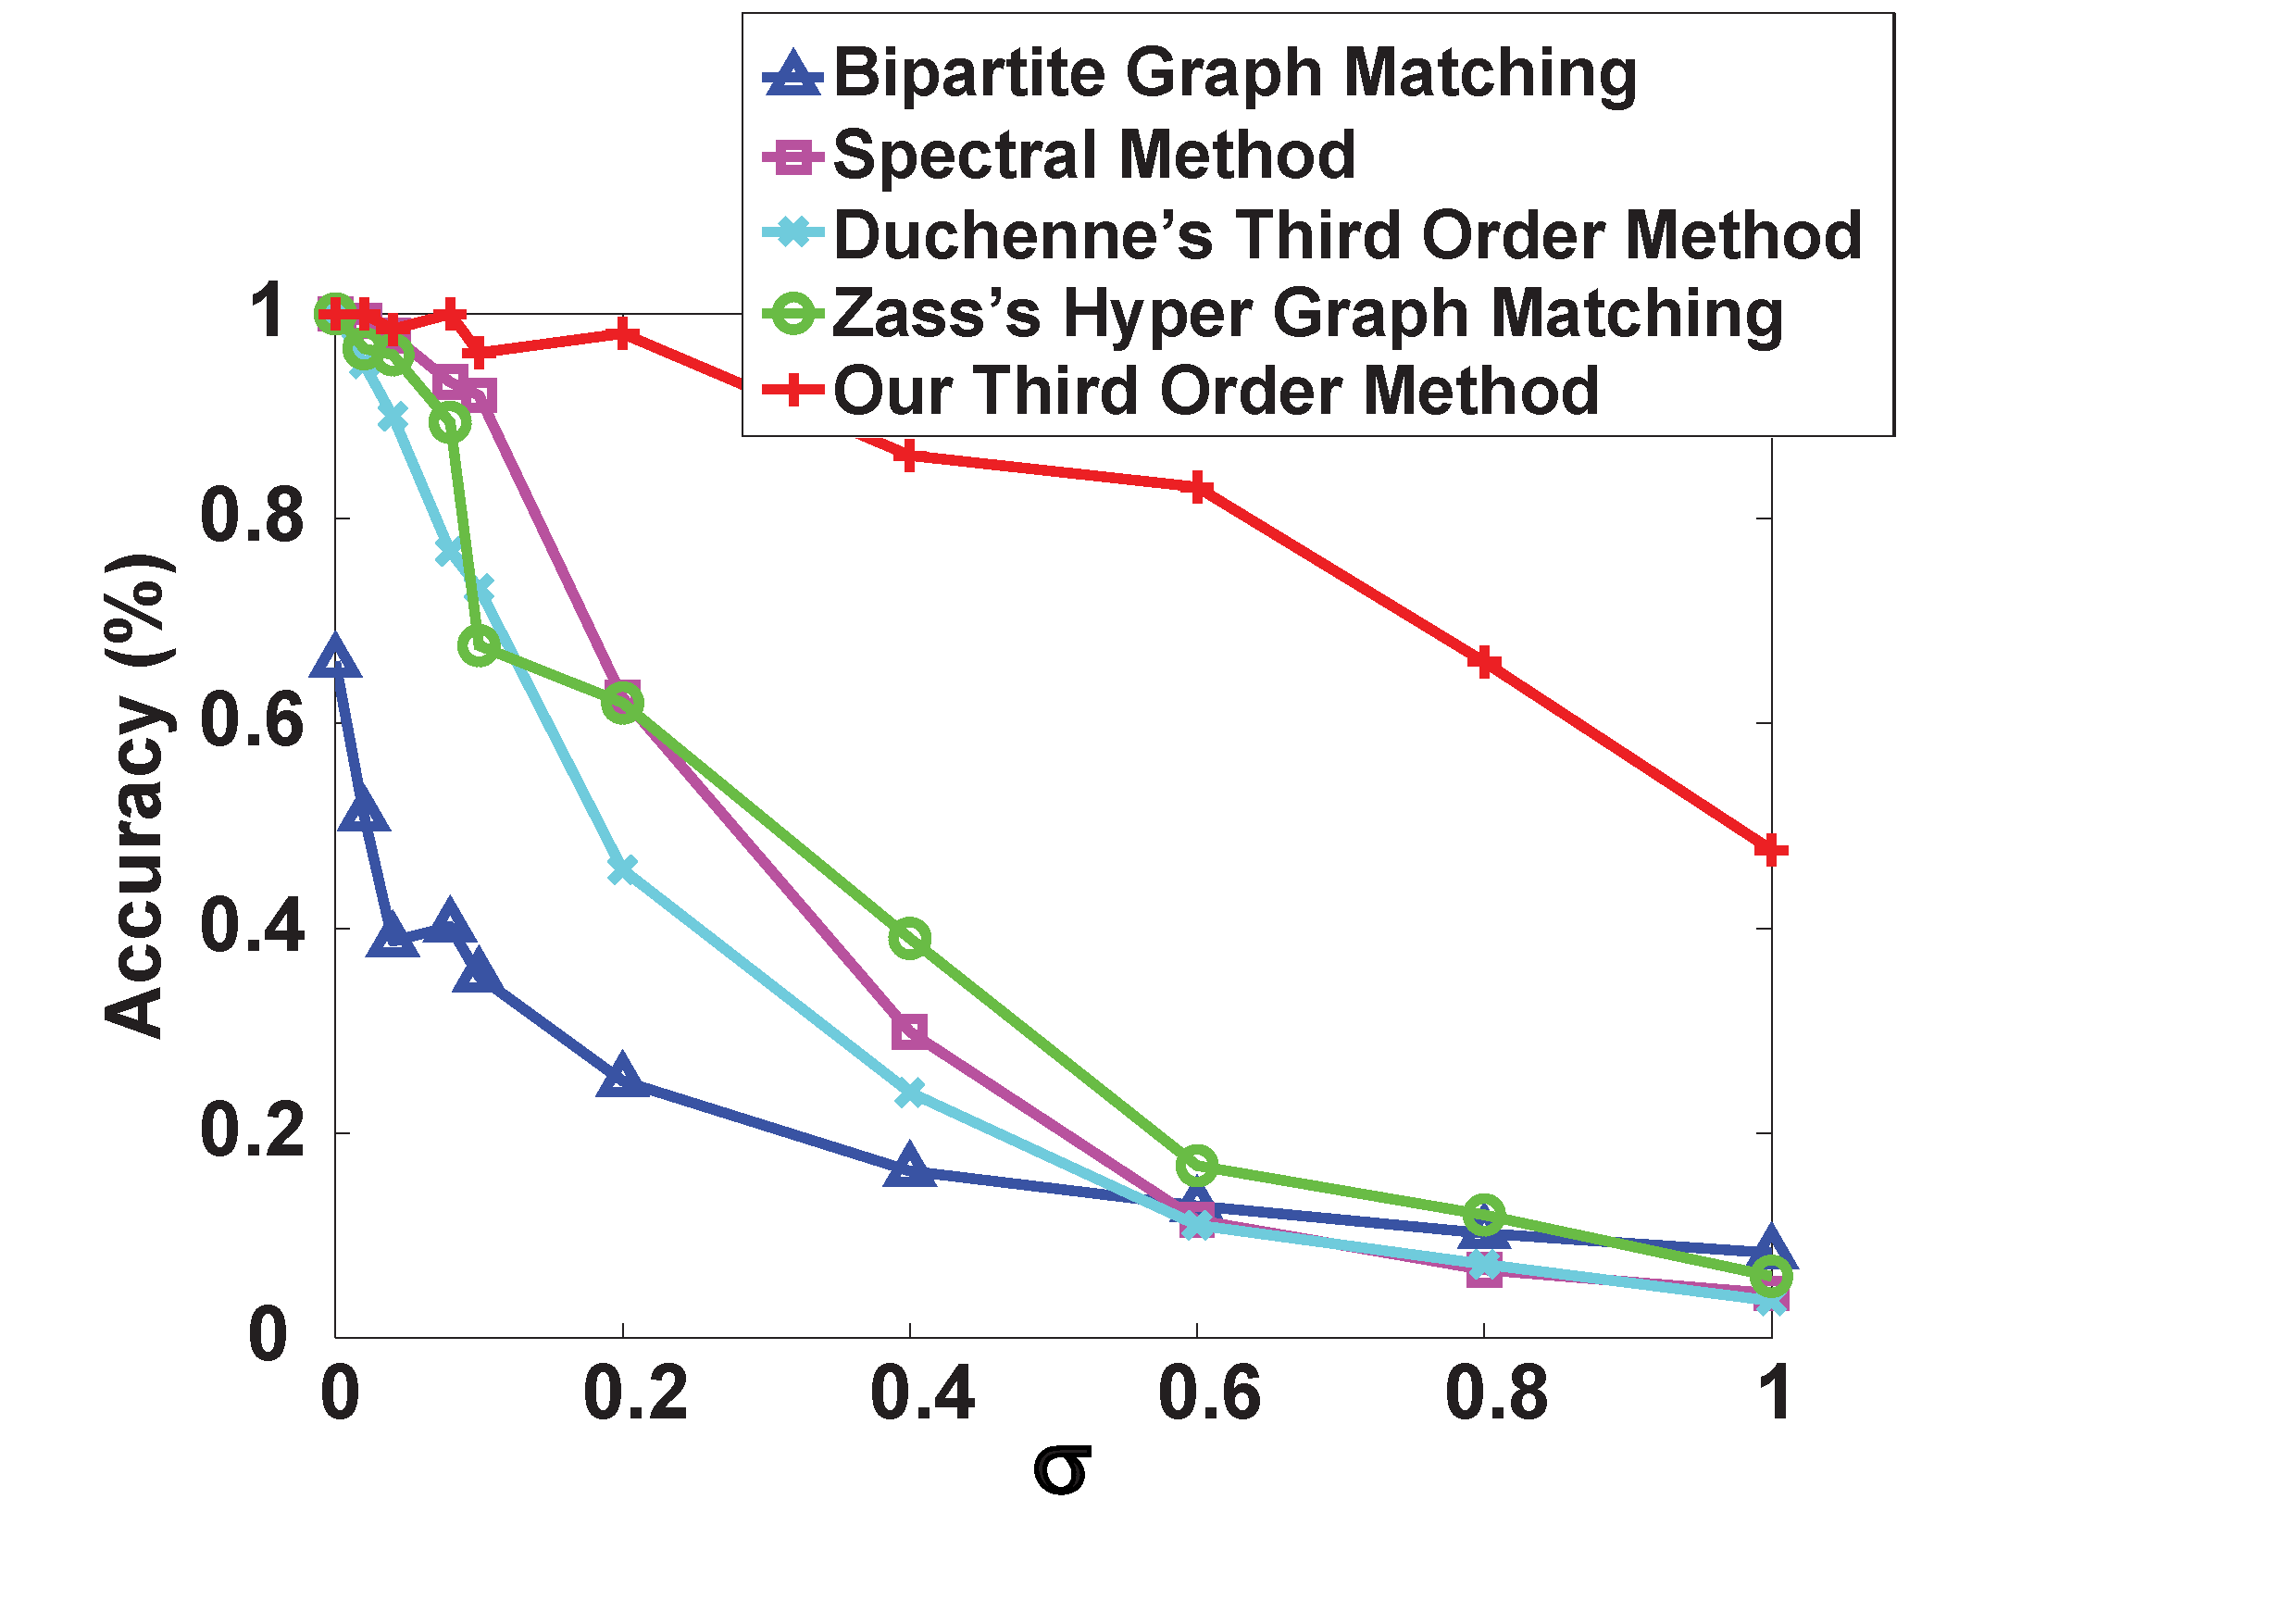
\includegraphics[width=63mm]{dtest_wide_embedded.pdf} }%
        \end{minipage}%
        \hspace{14mm}%
        %\addtocounter{subfigure}{-1}
        %----------------------------
        \begin{minipage}[b]{0.4\textwidth}
            \subfigure[]{
            \label{fig:subfig:otest}
            \centering
            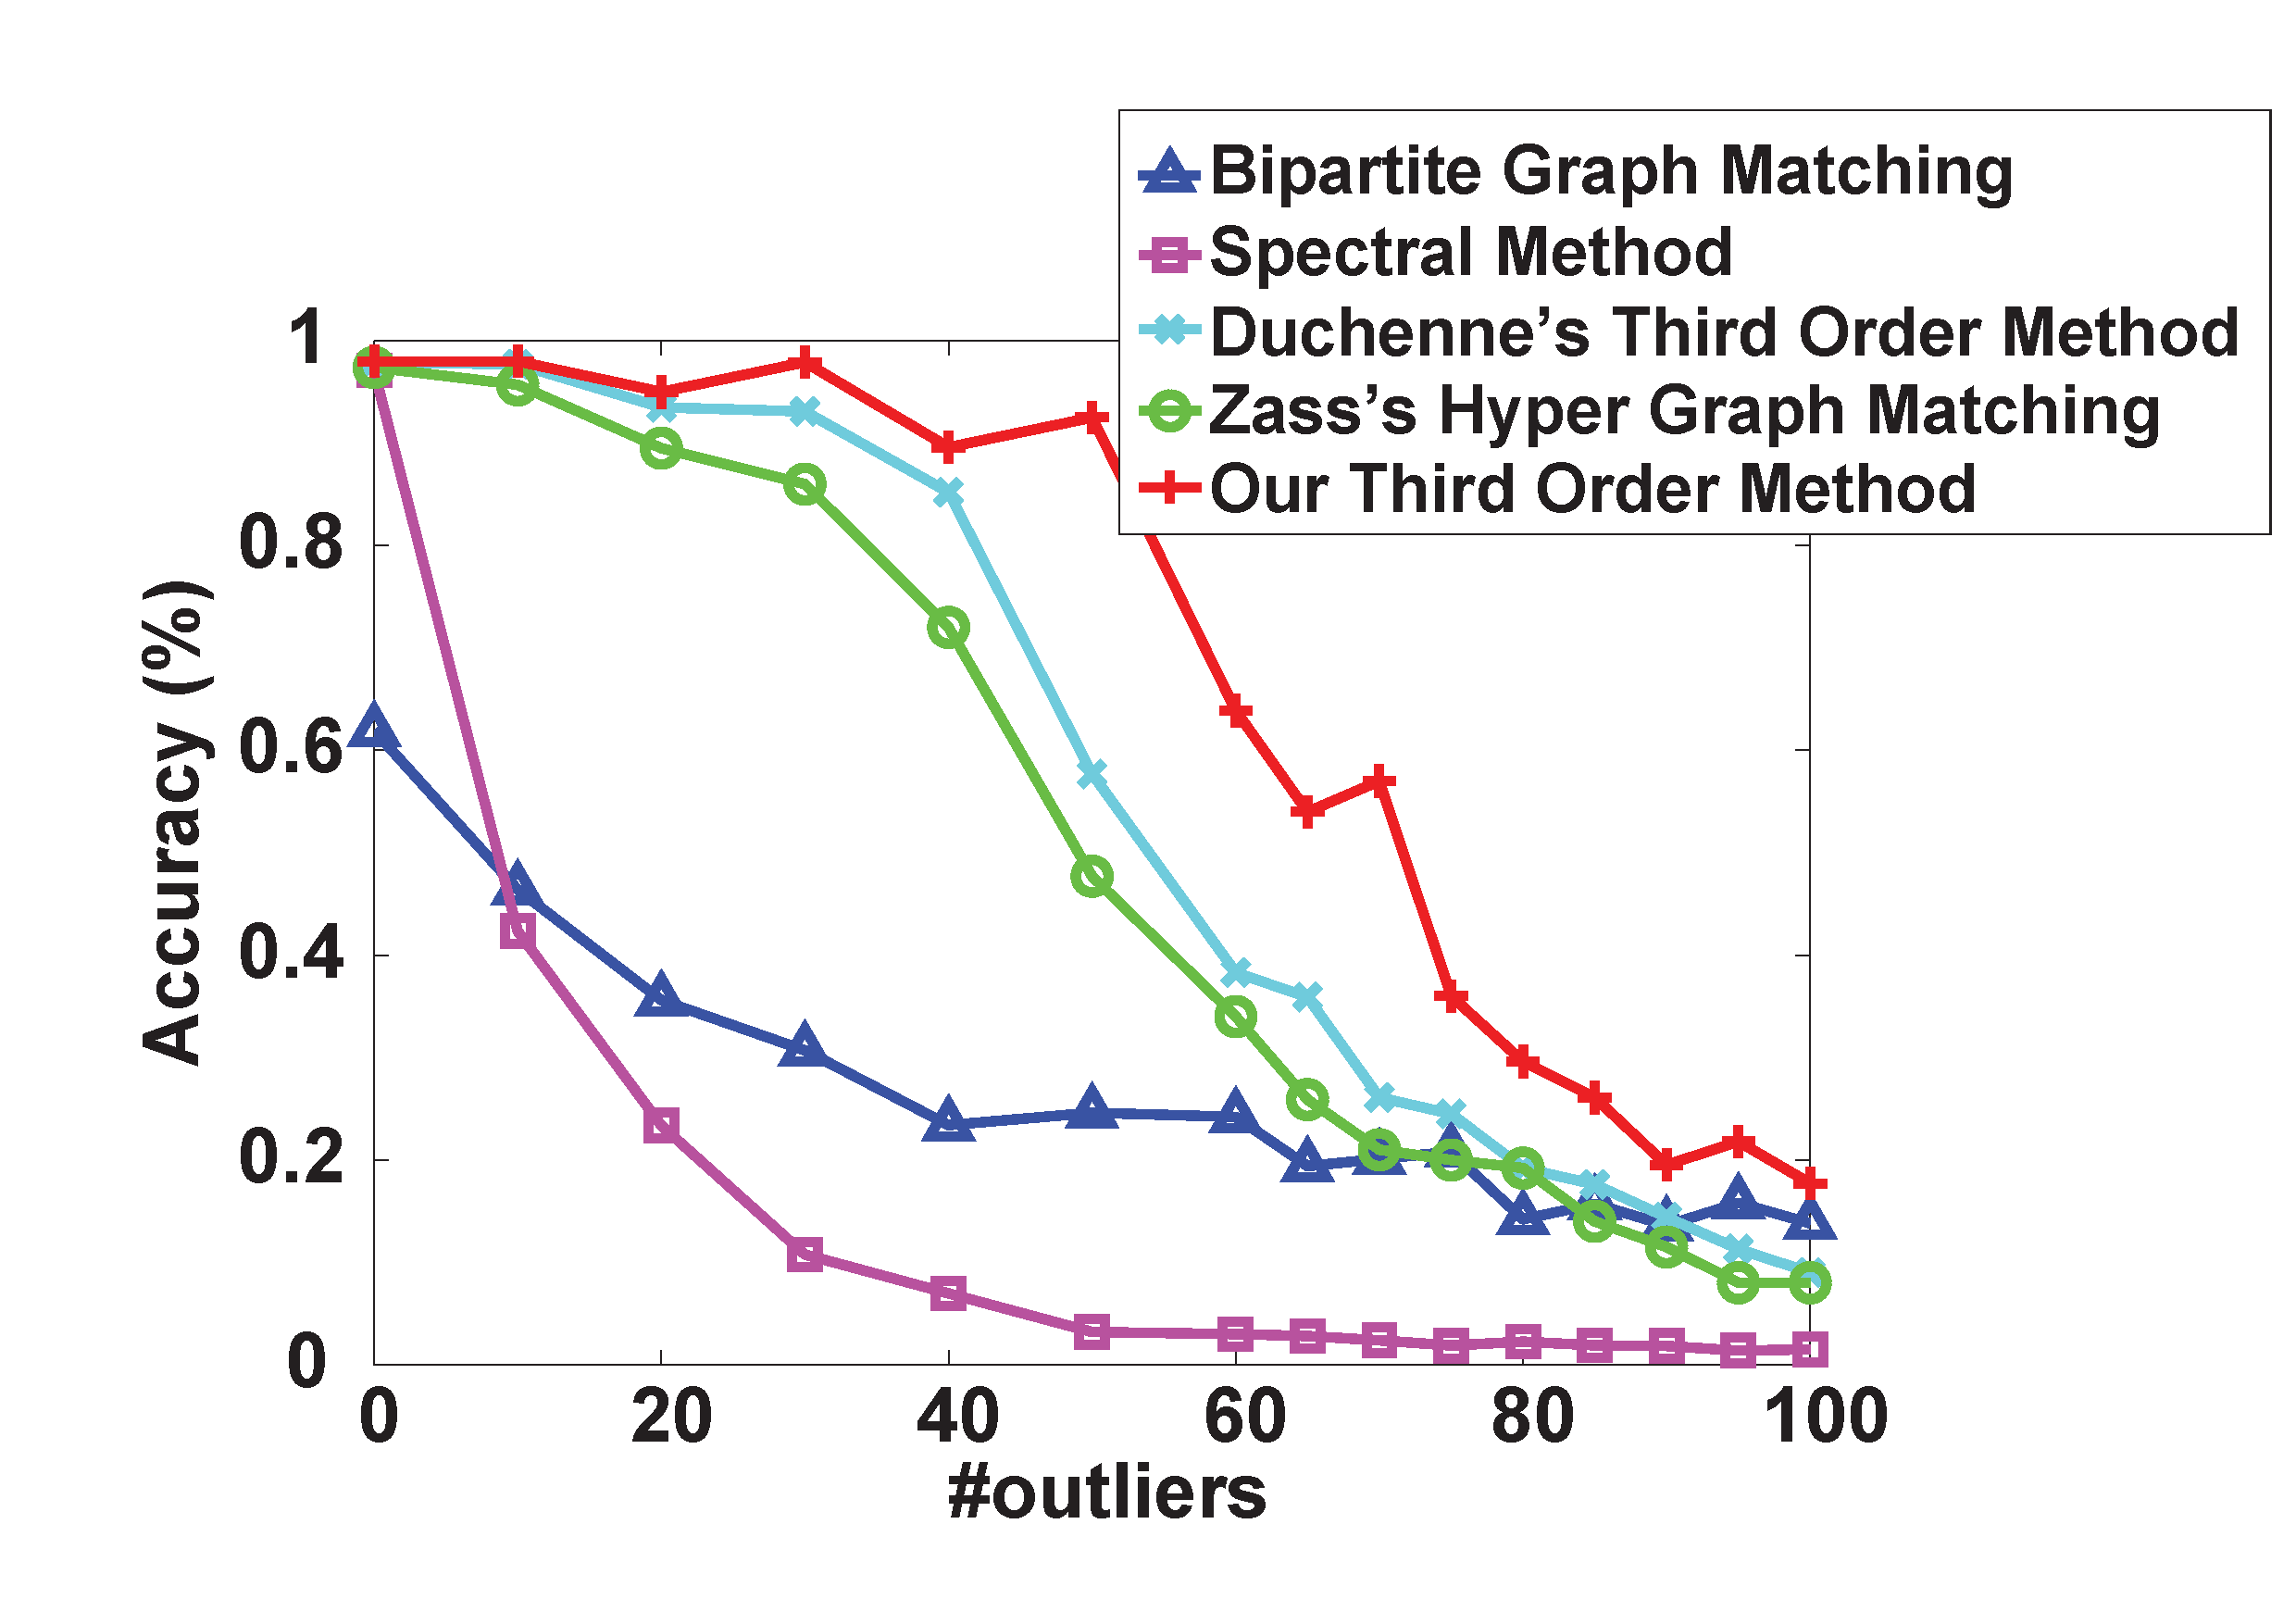
\includegraphics[width=70mm]{otest_embedded.pdf}}%
        \end{minipage}%
        %\hspace{10mm}%
        %\vspace{-4pt}%
        %\addtocounter{subfigure}{-1}
        \caption{Fig.\ref{fig:subfig:rtest} to \ref{fig:subfig:otest}, are the results of rotation test, rescaling test, distortion test and outlier test in the artificial data experiment. }
\label{fig:mini:subfig_part1} %% label for entire figure
\end{figure*}

We compared our third order method with all four other methods. Each test was executed 50 times, and we measured the matching accuracy as the number of correctly matched points divided by the total number of points that could potentially be matched. The mean accuracy over all experiments is given in Figures~\ref{fig:subfig:rtest}--\ref{fig:subfig:otest}. We can see that no matter how large the changes made to $P_1$ (in terms of rotation, rescaling, distortion and outliers ), our method could still find the correct correspondences, and outperforms other methods.
For larger amounts of rotation and scaling, the bipartite graph matching method~\cite{Belongie02} soon fails, while higher-order methods perform much better due to the addition of geometric constraints. However, the third order method in~\cite{Duchenne_etal09} and the hyper graph matching method do not perform so well, because the geometric relationships among elements are not established accurately. It is also clear that the spectral method~\cite{Cour06} cannot deal with large scale factors.

To provide a fair comparison, the number of tensor elements generated in our method, \cite{Duchenne_etal09} and \cite{Zass08} were kept the same in all four tests (but different numbers were used for each method).
In the first three tests, our method used 5000 feature tuples from $P_1$ and $P_2$ is $5000$, while $150000$ were used for~\cite{Duchenne_etal09} and $10000$ for~\cite{Zass08}. The number of feature tuples used in the outlier test were equivalent for our method, \cite{Duchenne_etal09} and \cite{Zass08}.

Matching two feature sets each with $50$ features took an average of about $1.8$s\footnote{All methods were implemented in Matlab on a $2.3$GHz Core2Duo with $2$GB memory.} for our method, $2.6$s for \cite{Duchenne_etal09}, $0.9$s for~\cite{Zass08}, $0.37$s for~\cite{Cour06}, and $0.18$s for~\cite{Belongie02}. As we use the same tensor size but sample fewer feature tuples, we achiev a higher matching accuracy with less computation than~\cite{Duchenne_etal09} and~\cite{Zass08}.

%-------------------------------------------------------------------------
\subsection{Image matching under affine transformation}
\label{subsec:affinedata}

Matching images related by an affine transformation is an important task. We used two publicly available image sets, \texttt{graf} and \texttt{wall}\footnote{From \url{http://www.robots.ox.ac.uk/~vgg/data/data-aff.html}}, to evaluate the matching accuracy of our method under affine transformations. These image sets each contain 6 images of a planar wall, which we numbered 1--6. For each image set, we used features generated from image 1 to match features in images 2 to 6 separately.

For the test image sets, we used $30$ feature points detected by MSER~\cite{Matas04} in the central area of image 1 to be feature set $P_1$ (the green points in Fig.\ref{fig:subfig:wallimage1}). We then used the the transformation matrices provided with the image sets to find corresponding points for the feature set $P_2$ for images 2--6.
In order to assess the robustness of the algorithms, we manually added outliers to $P_1$, shown as yellow points in Fig.\ref{fig:subfig:wallimage1}. We successively increased the number of outliers until the ratio of outliers was 1/3.

For this test, we compared our method with the spectral method~\cite{Cour06} (a pairwise method), a tensor based method~\cite{Duchenne_etal09} and the hypergraph matching method~\cite{Zass08}, using the same fourth-order potentials for the higher-order methods. Method~\cite{Duchenne_etal09},~\cite{Zass08} and ours used an equivalent tensor size. In each test, $6000$ feature tuples were used in our method, $813000$ for~\cite{Duchenne_etal09} and $12000$ for~\cite{Zass08}.
%
%-------------------------------------------
%  just two model images  from graf and wall
%-------------------------------------------
\begin{figure*}[!t]
%\vspace{-4mm}
%\hspace{-8ex}
\setlength{\abovecaptionskip}{0mm}
\setlength{\belowcaptionskip}{-2mm}
\centering
\setlength\subfigcapskip{-2mm}
\hspace{-5ex}
         \begin{minipage}[b]{0.4\textwidth}
            \subfigure[]{
            \label{fig:subfig:grafimage1}
            \centering
            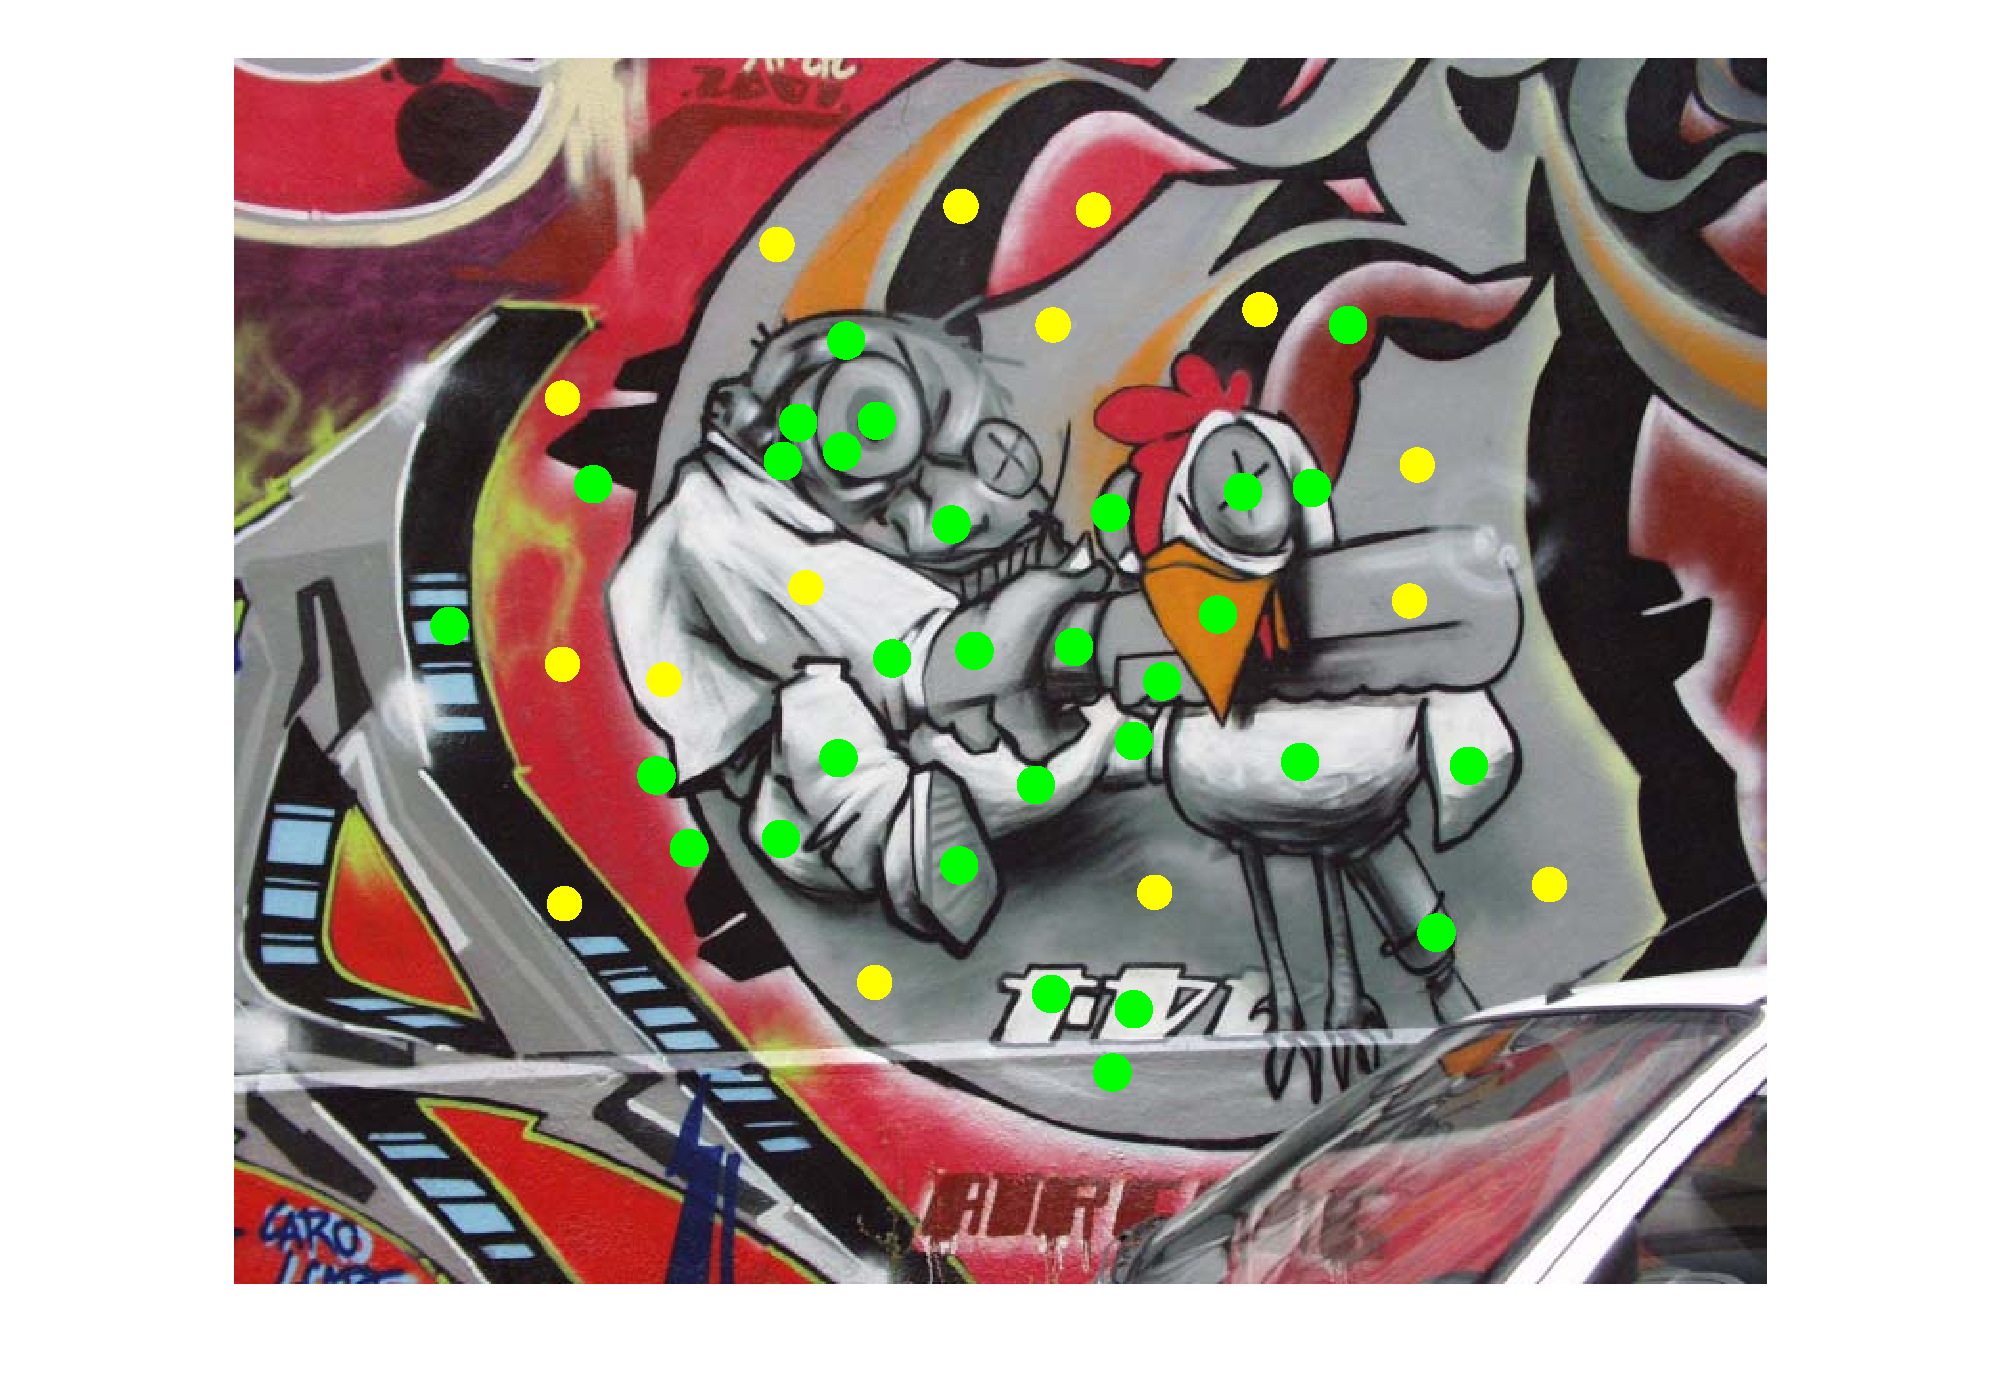
\includegraphics[width=56mm]{graf-NoiseSet.pdf}}%
        \end{minipage}%
         \hspace{10mm}%
         \begin{minipage}[b]{0.4\textwidth}
            \subfigure[]{
            \label{fig:subfig:wallimage1}
            \centering
            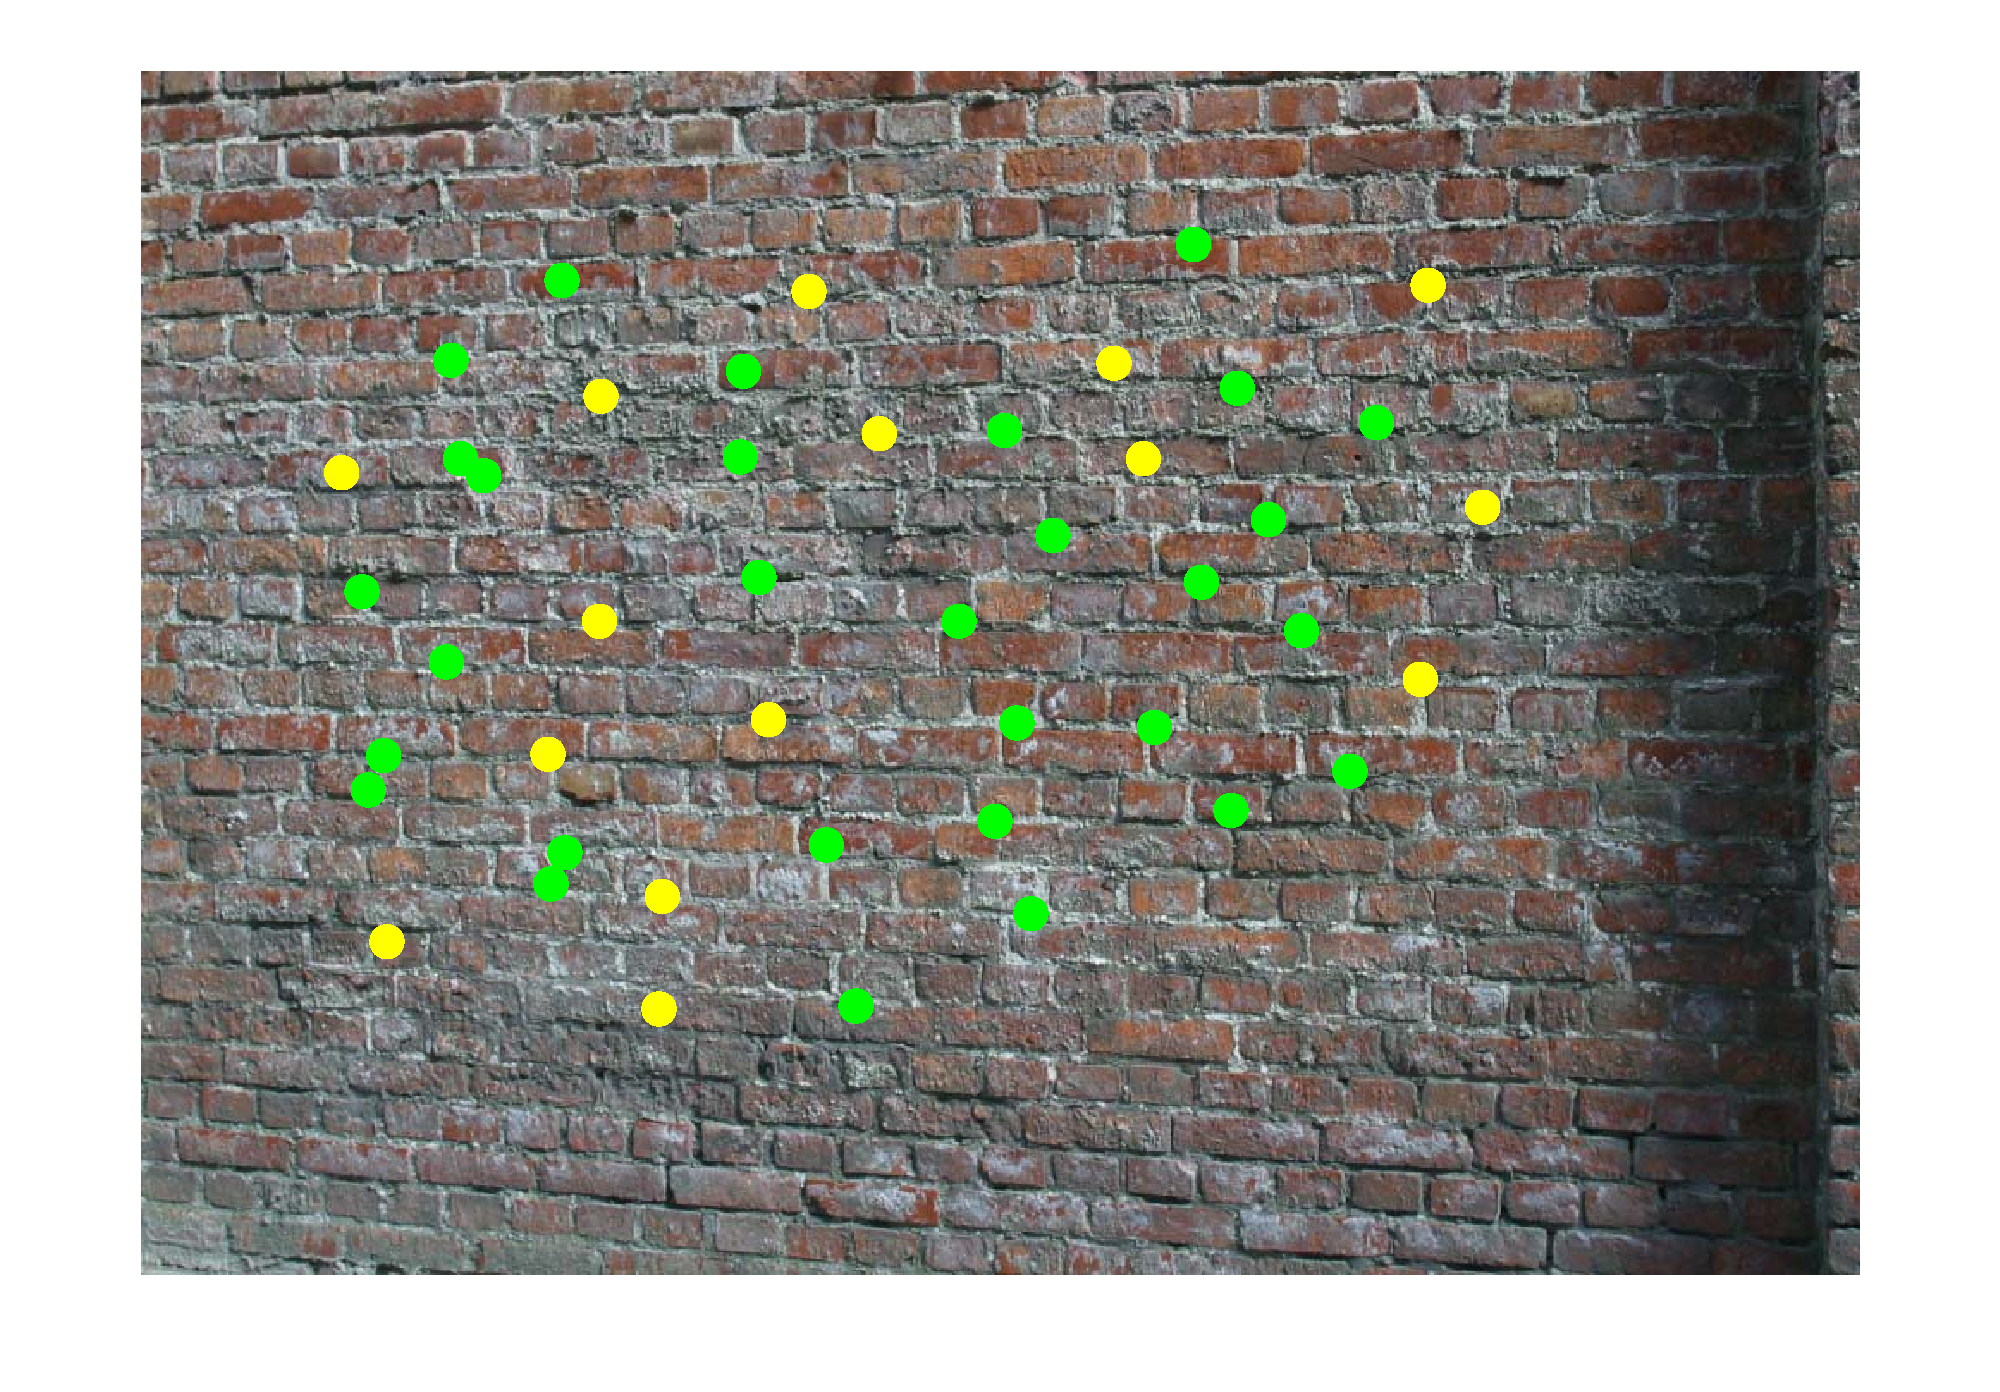
\includegraphics[width=64mm]{wall-noisedataset.pdf}}%
        \end{minipage}%
        %\addtocounter{subfigure}{-1}
        \caption{Left: image 1 in \texttt{graf} set, right: image 1 in \texttt{wall} set. Model features detected by MSER in image 1 are shown in green; yellow points are outliers.}
\label{fig:mini:subfig_affinematching1} %% label for entire figure
\end{figure*}%
%-----------------------------------
%  error rate for both graf and wall
%-----------------------------------
\begin{figure*}[!htp]
%\vspace{-4mm}
%\hspace{-8ex}
\setlength{\abovecaptionskip}{0mm}
\setlength{\belowcaptionskip}{0mm}
\centering
\setlength\subfigcapskip{-2mm}
\hspace{-8ex}
\vspace{-2mm}
         %----------------------------
         %%% smac method
         %----------------------------
         \begin{minipage}[b]{0.4\textwidth}
         \subfigure{
            \label{fig:subfig:graferror1}
            \centering
            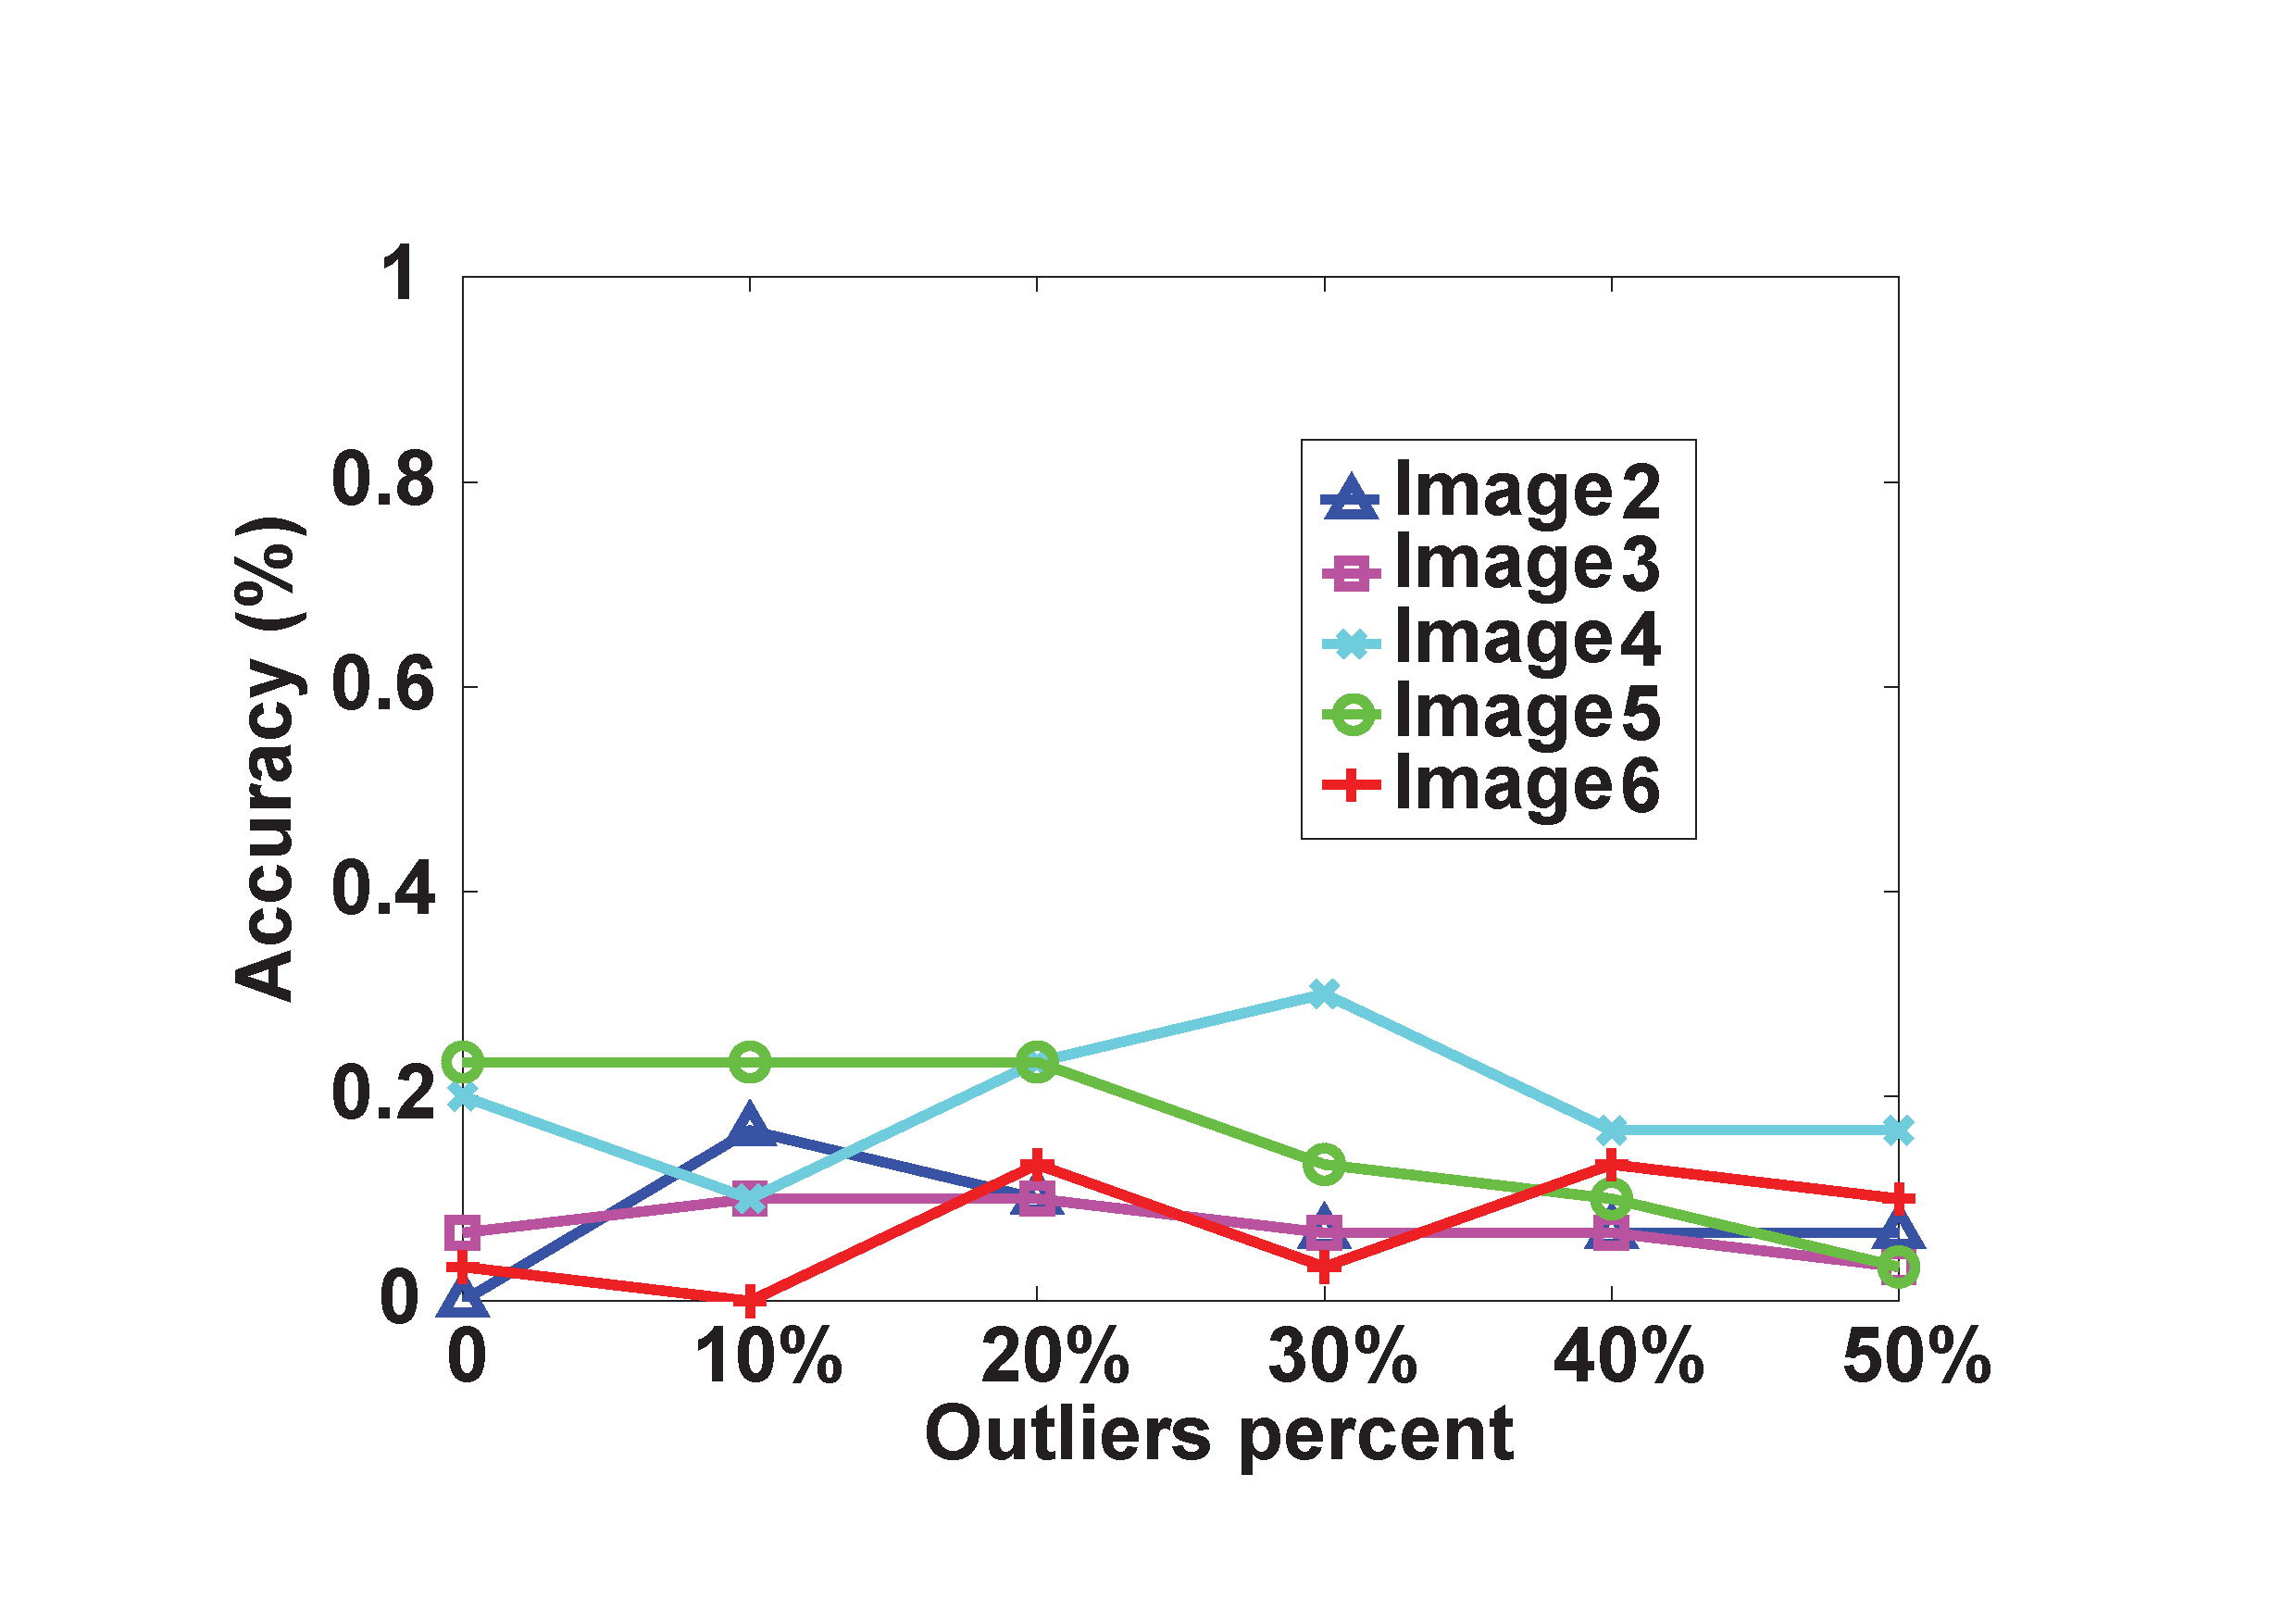
\includegraphics[width=58mm]{graf_SMAC_ERRORRATE_embedded.pdf}%
            }%
        \end{minipage}%
        \hspace{10mm}%
        \addtocounter{subfigure}{-1}
        %----------------------------
        \begin{minipage}[b]{0.4\textwidth}
         \subfigure{
            \label{fig:subfig:wallerror1}
            \centering
            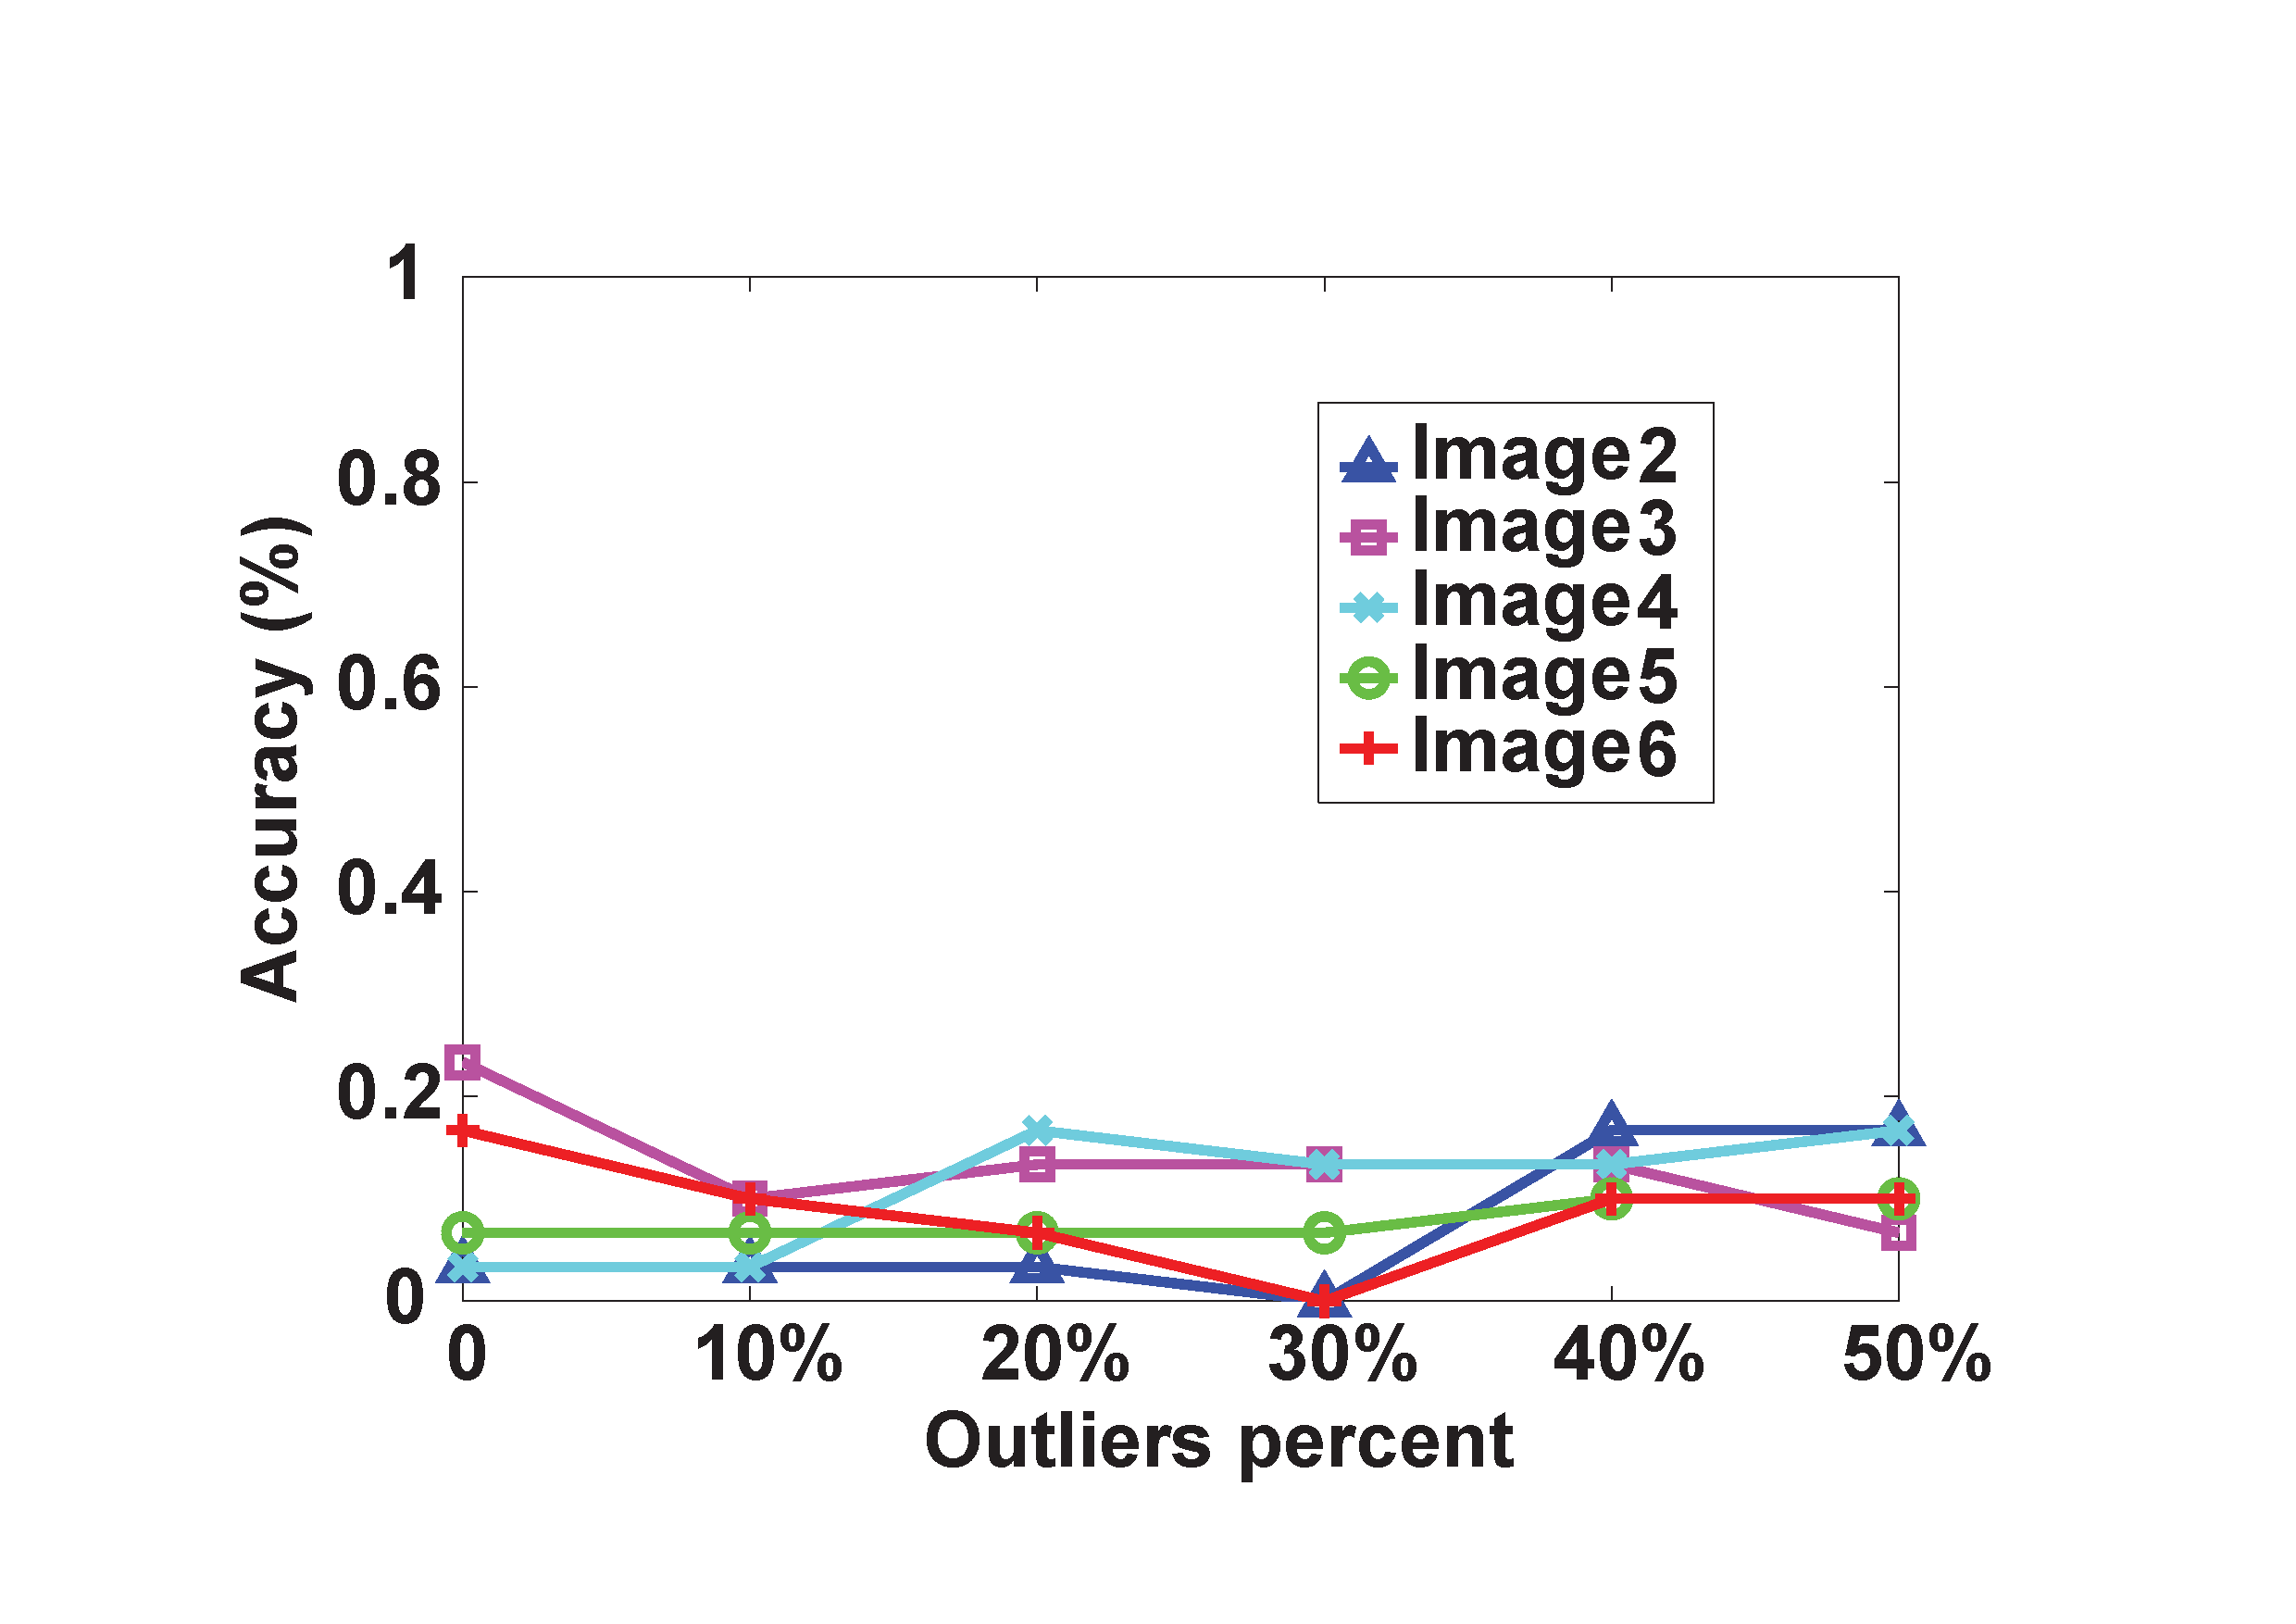
\includegraphics[width=58mm]{wall_SMAC_ERRORRATE_embedded.pdf}%
            }%
        \end{minipage}\\%
        \vspace{-2mm}%
        \addtocounter{subfigure}{-1}
        %----------------------------
        %%% hyper method
        %----------------------------
        \hspace{-8ex}
        \begin{minipage}[b]{0.4\textwidth}
        \subfigure{
            \label{fig:subfig:graferror2}
            \centering
            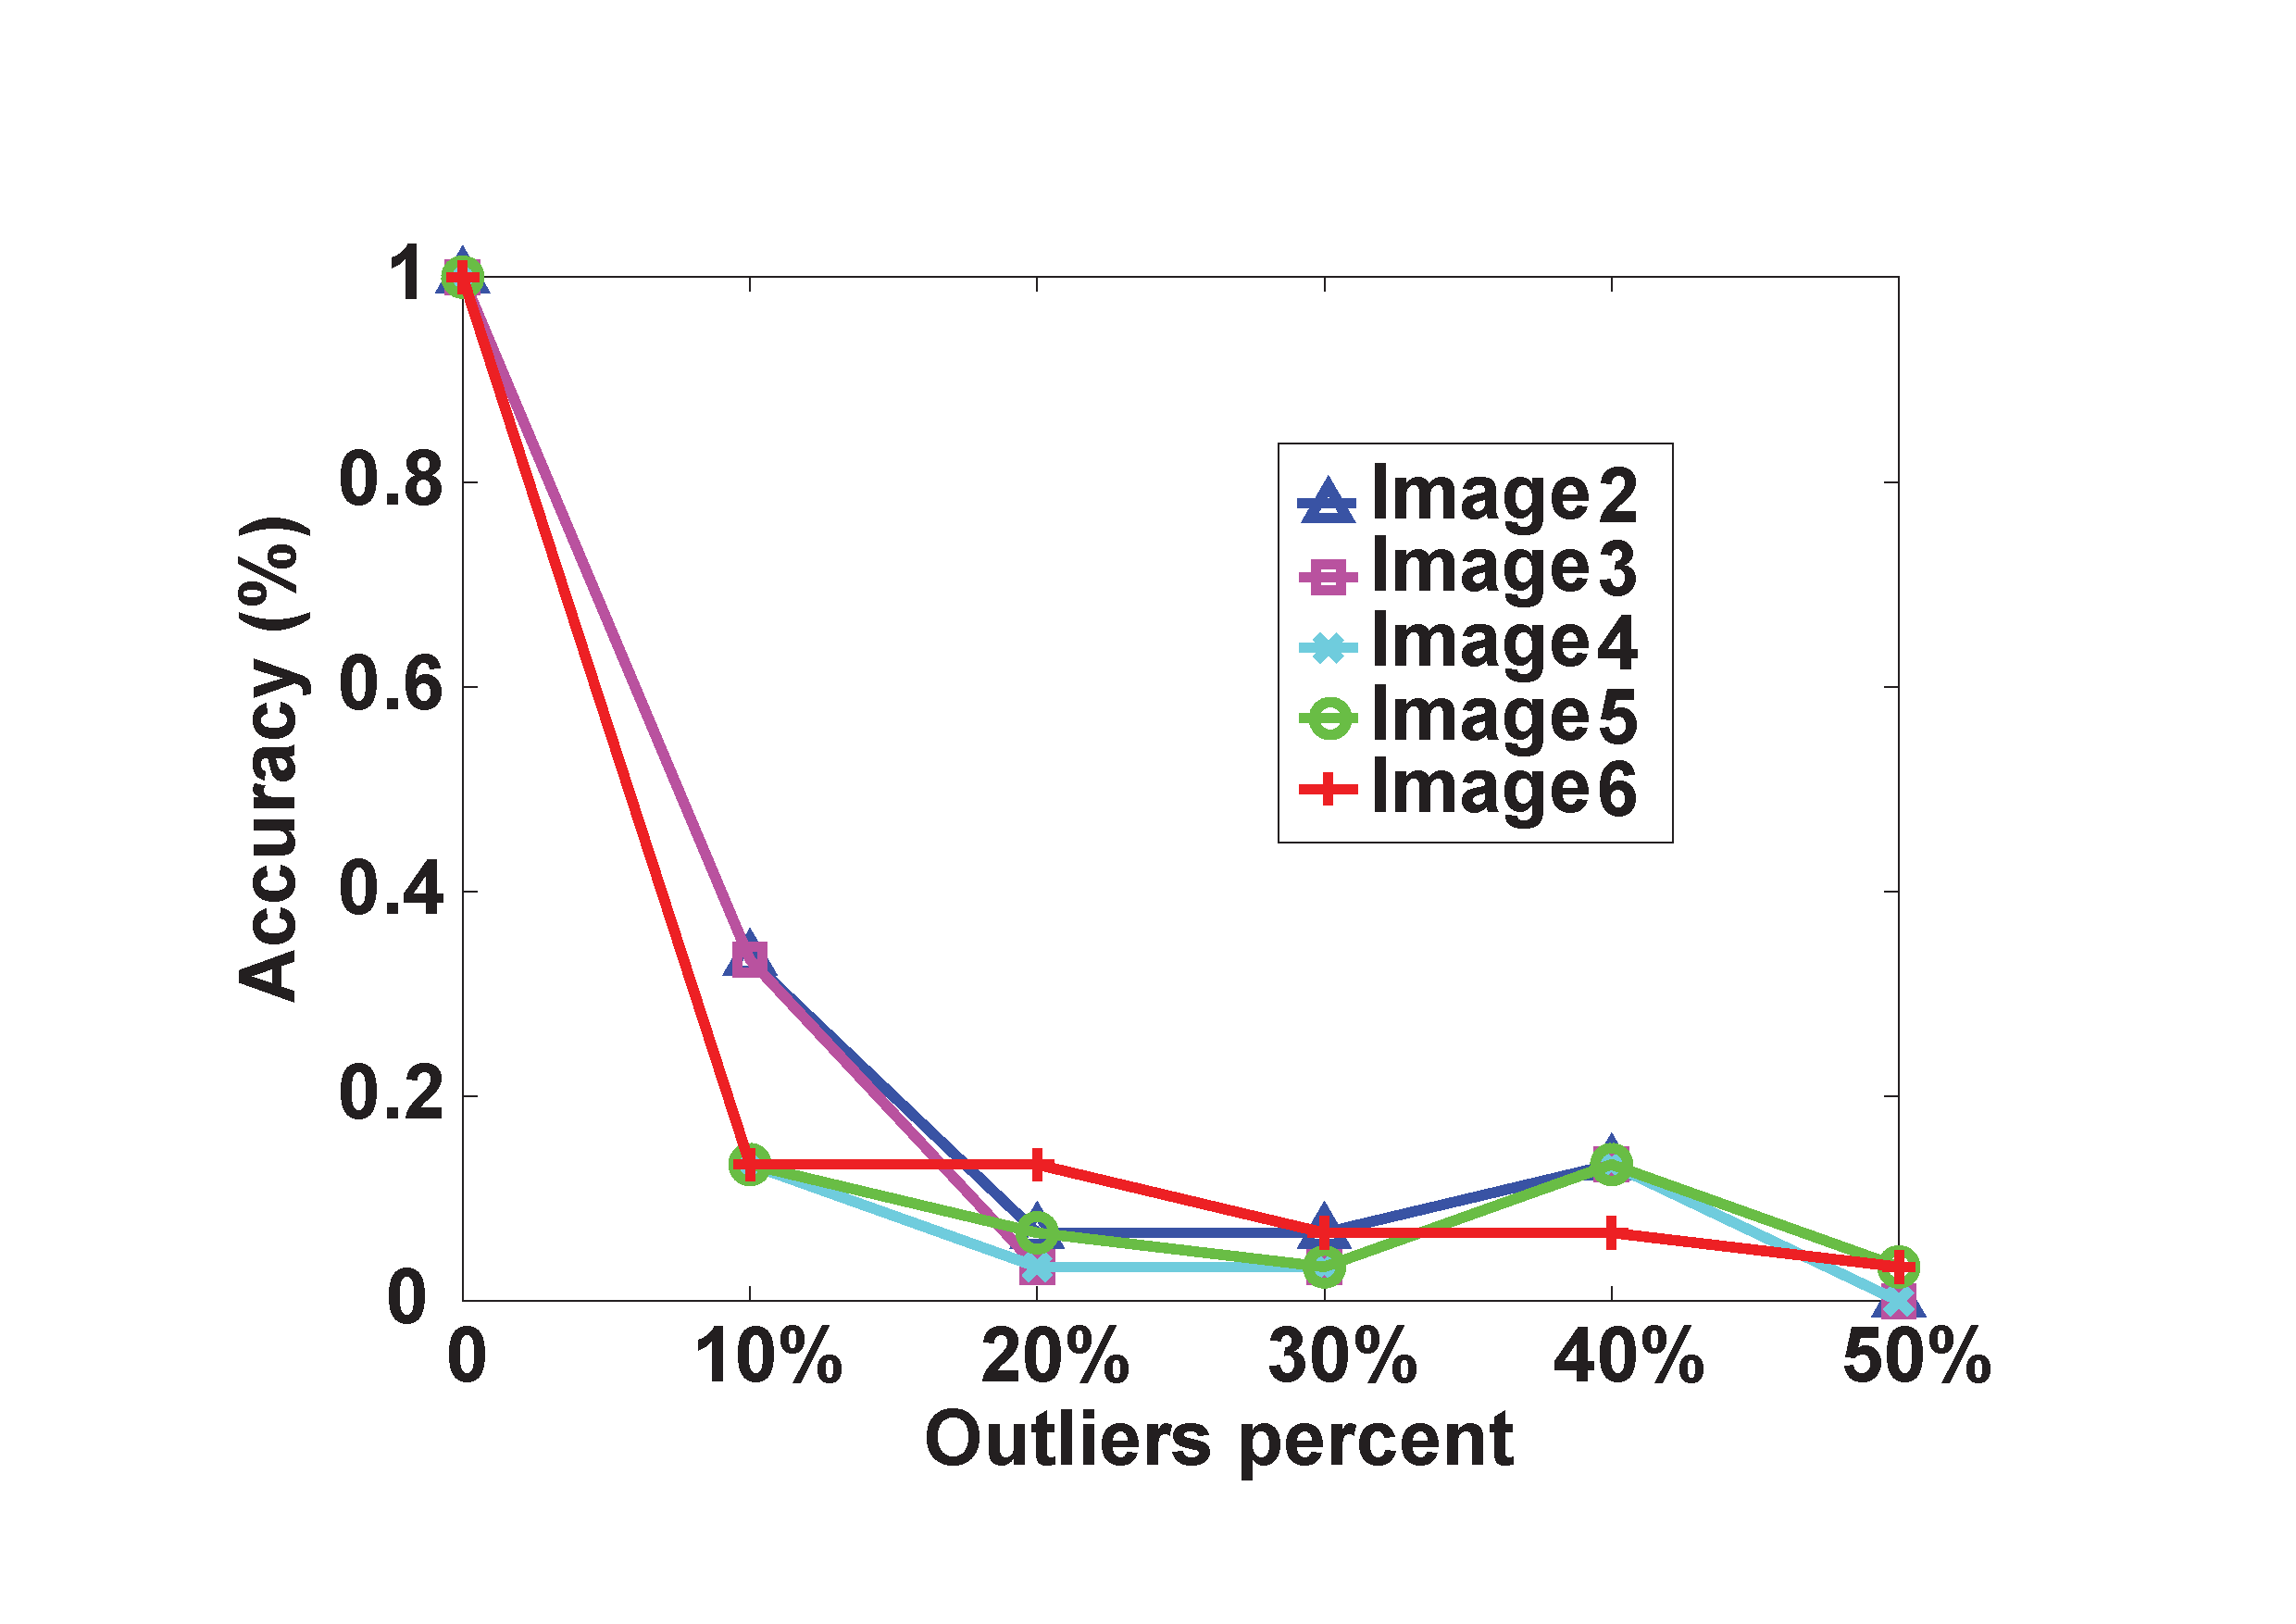
\includegraphics[width=58mm]{graf_HYPER_ERRORRATE_embedded.pdf}%
            }%
        \end{minipage}%
        \hspace{10mm}%
        \addtocounter{subfigure}{-1}
        %----------------------------
        \begin{minipage}[b]{0.4\textwidth}
        \subfigure{
            \label{fig:subfig:wallerror2}
            \centering
            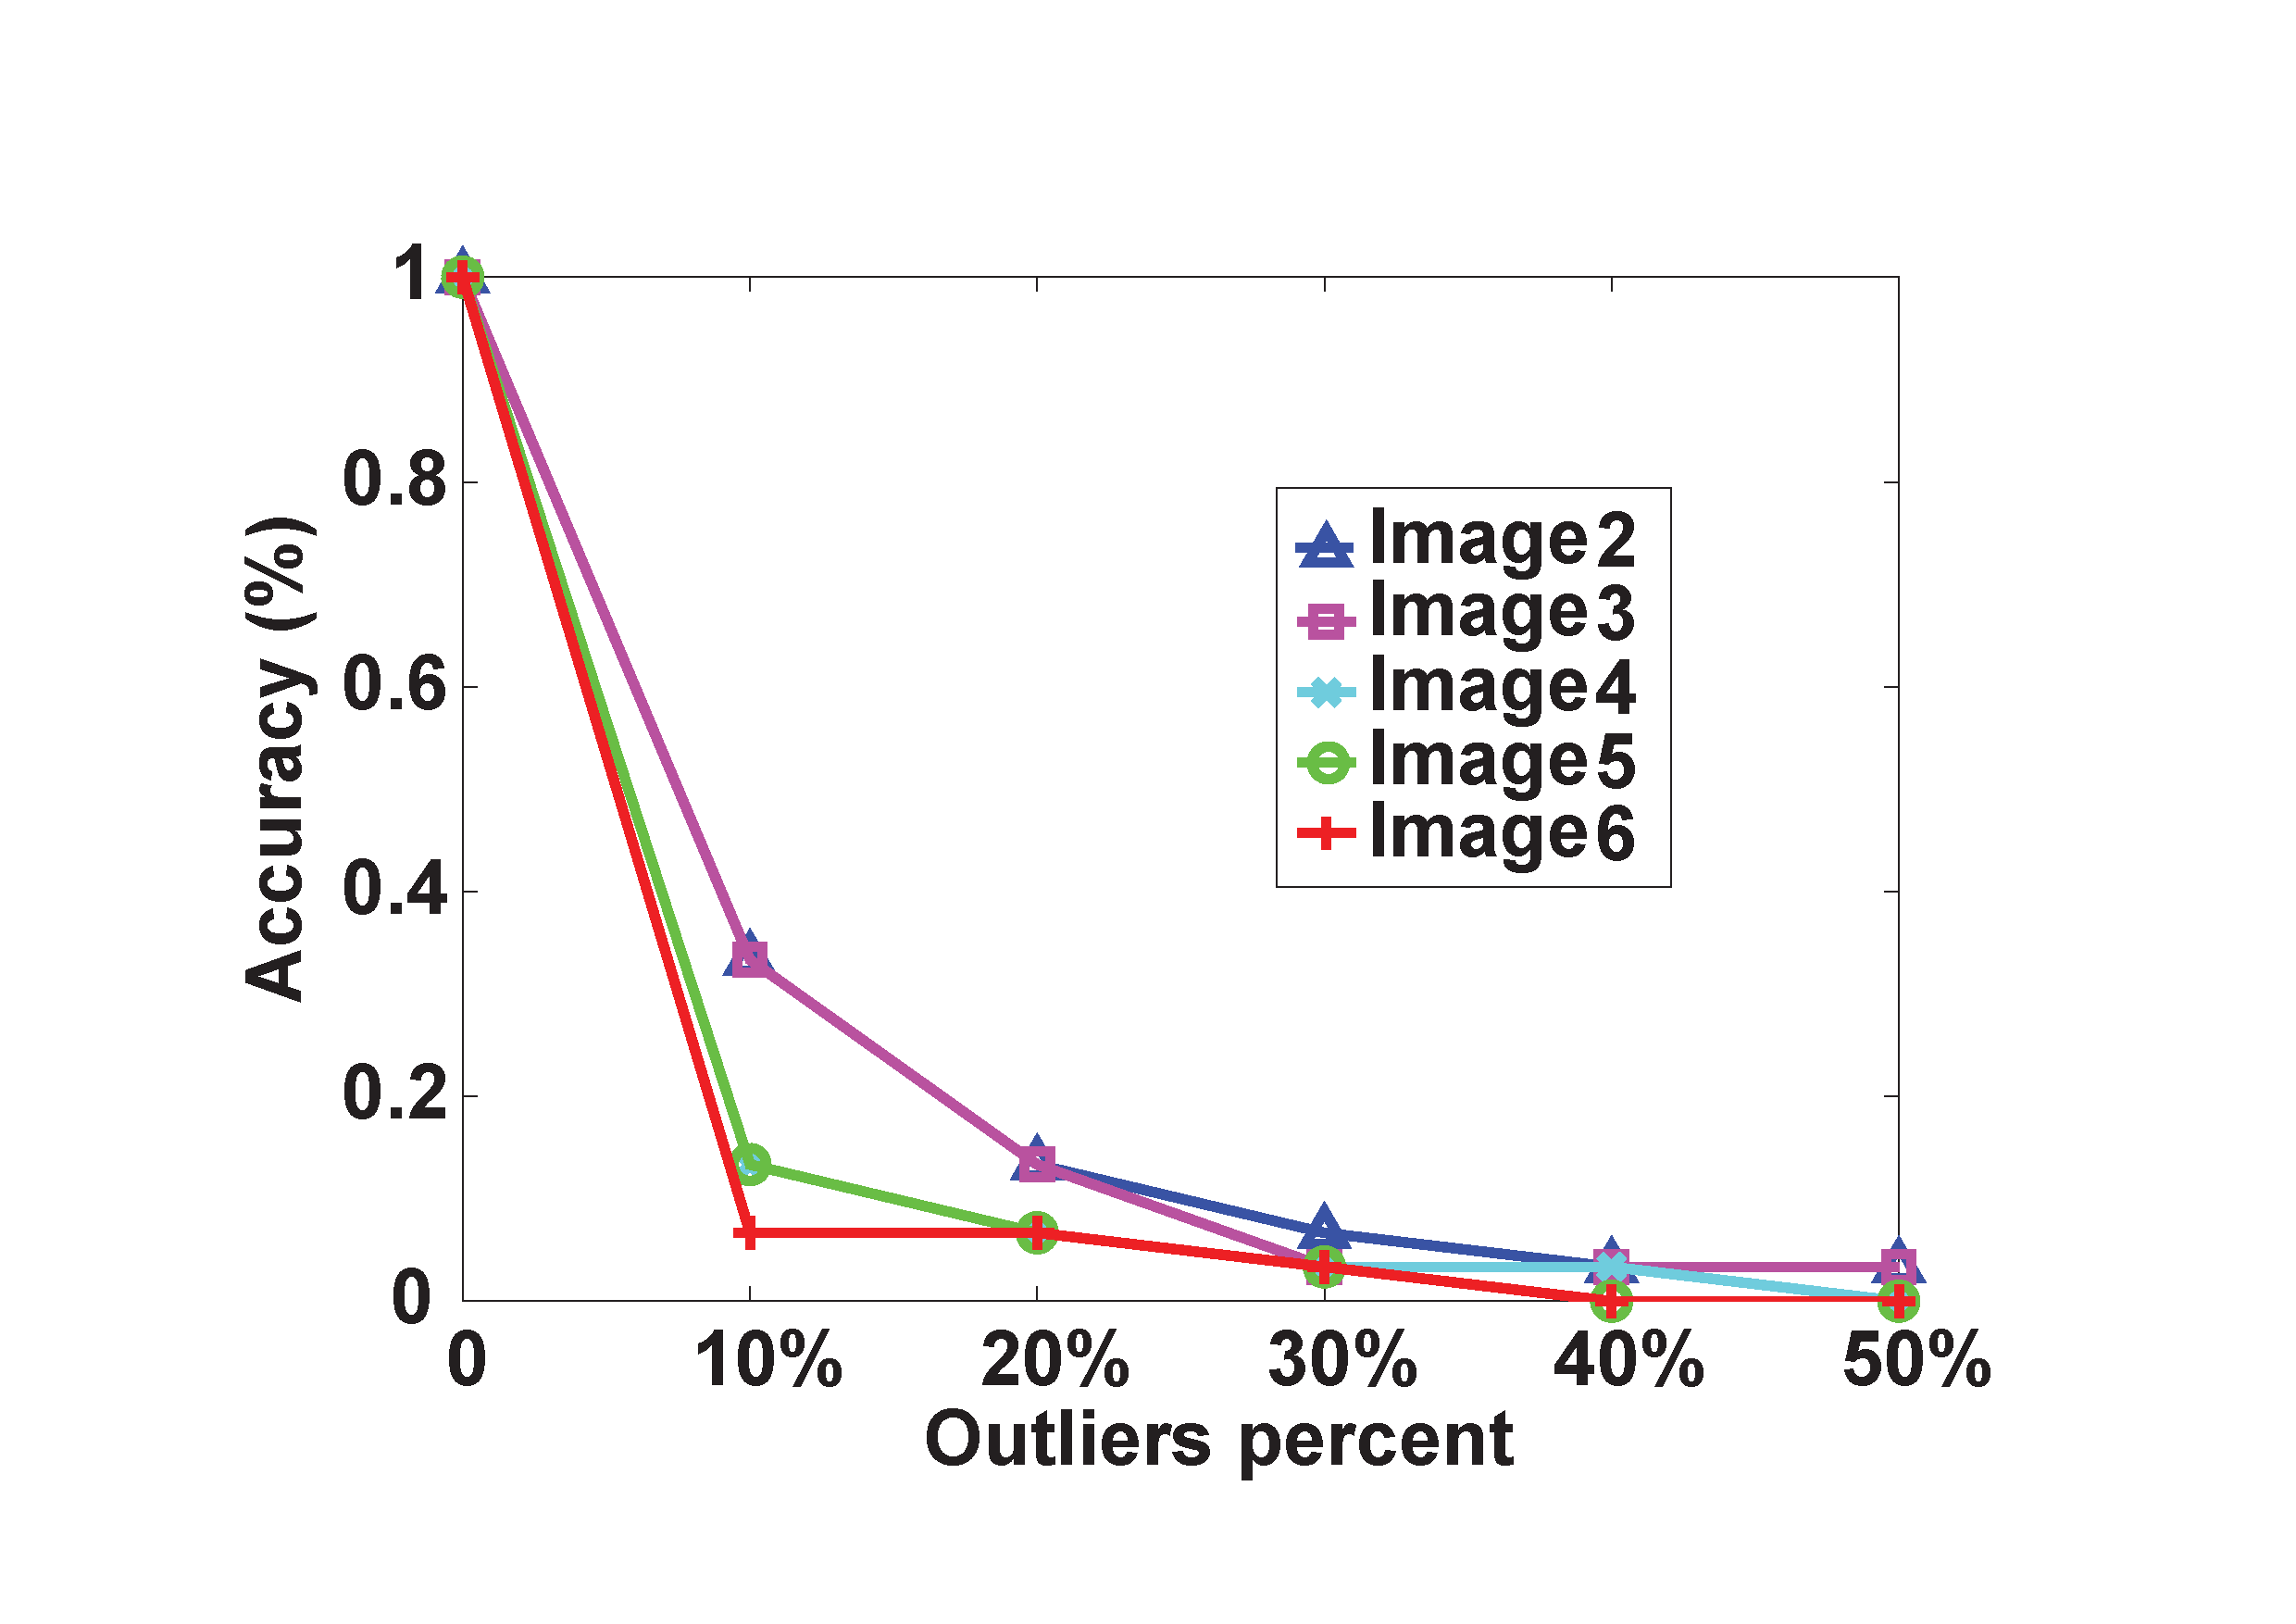
\includegraphics[width=58mm]{wall_HYPER_ERRORRATE_embedded.pdf}%
            }%
        \end{minipage}\\%
        \vspace{-2mm}%
        \addtocounter{subfigure}{-1}
        %----------------------------
        %%% orignal third method
        %----------------------------
        \hspace{-8ex}
        \begin{minipage}[b]{0.4\textwidth}
        \subfigure{
            \label{fig:subfig:graferror3}
            \centering
            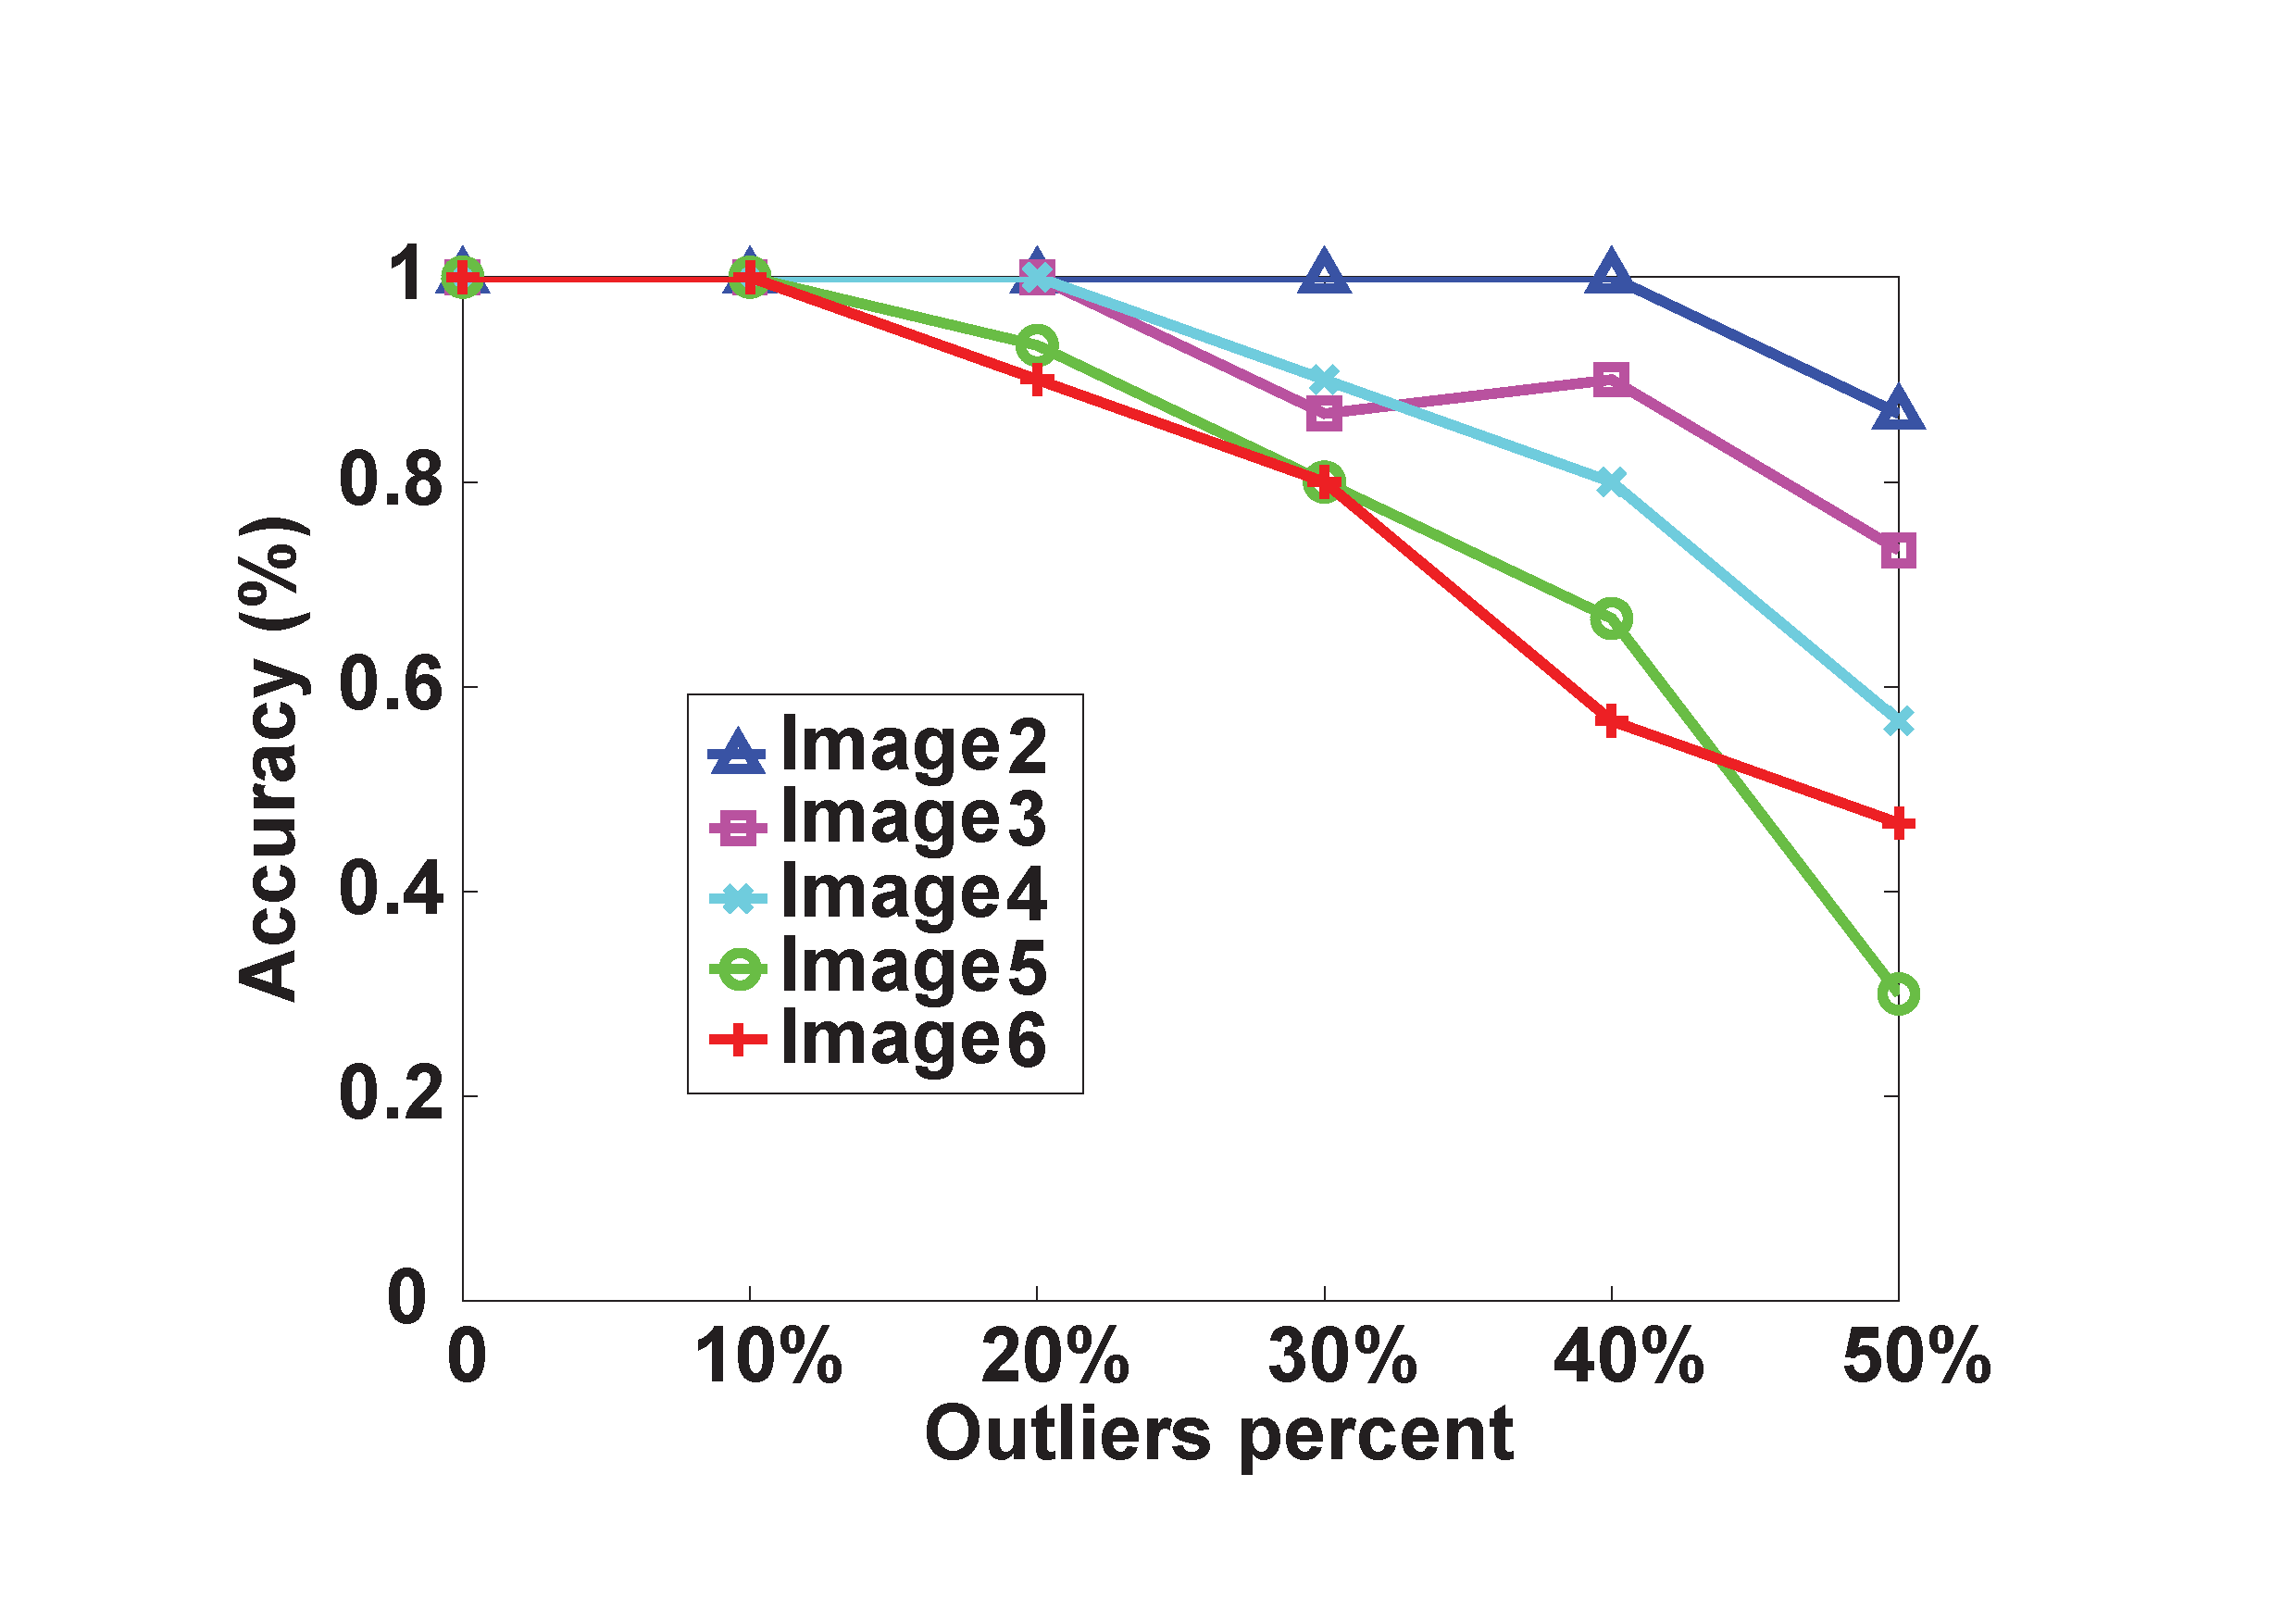
\includegraphics[width=58mm]{graf_DEMO_ERRORRATE_embedded.pdf}%
            }%
        \end{minipage}%
         \hspace{10mm}%
         \addtocounter{subfigure}{-1}
         %----------------------------
         \begin{minipage}[b]{0.4\textwidth}
         \subfigure{
            \label{fig:subfig:wallerror3}
            \centering
            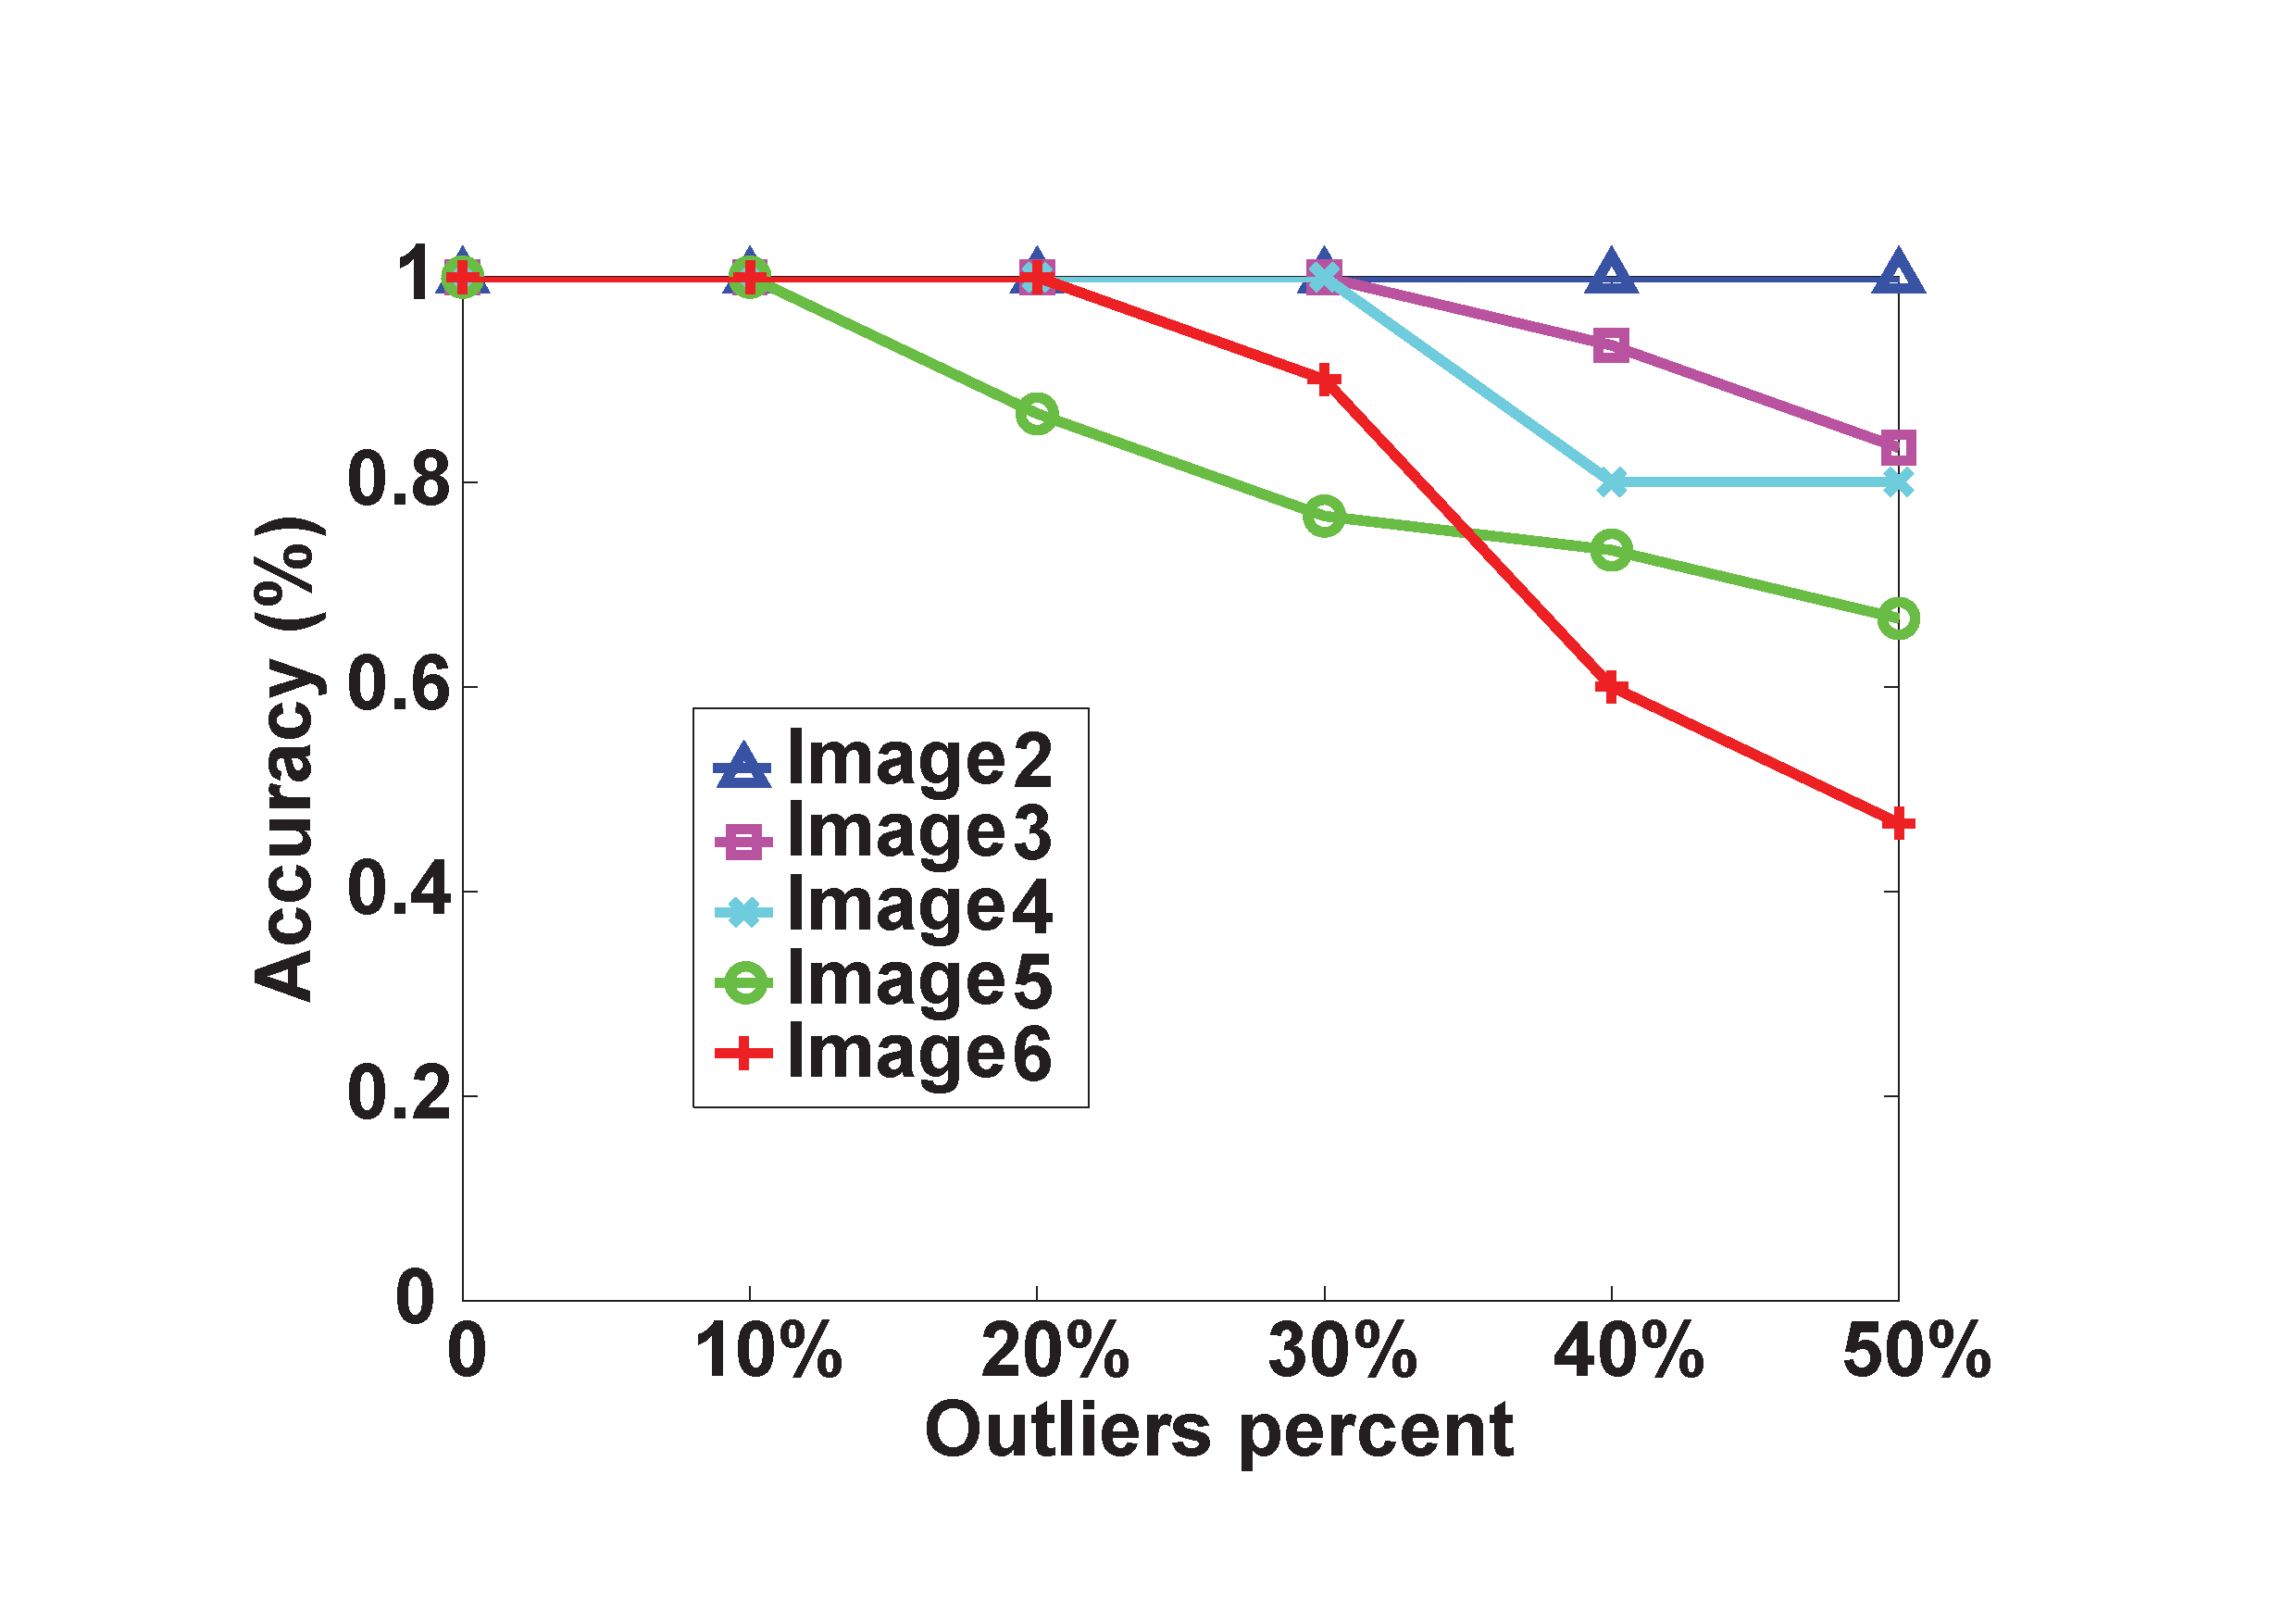
\includegraphics[width=58mm]{wall_DEMO_ERRORRATE_embedded.pdf}%
            }%
        \end{minipage}\\%
        \vspace{-2mm}%
        \addtocounter{subfigure}{-1}
        %----------------------------
        %%% our method
        %----------------------------
        \hspace{-8ex}
        \begin{minipage}[b]{0.4\textwidth}
        \subfigure[]{
            \label{fig:subfig:graferror4}
            \centering
            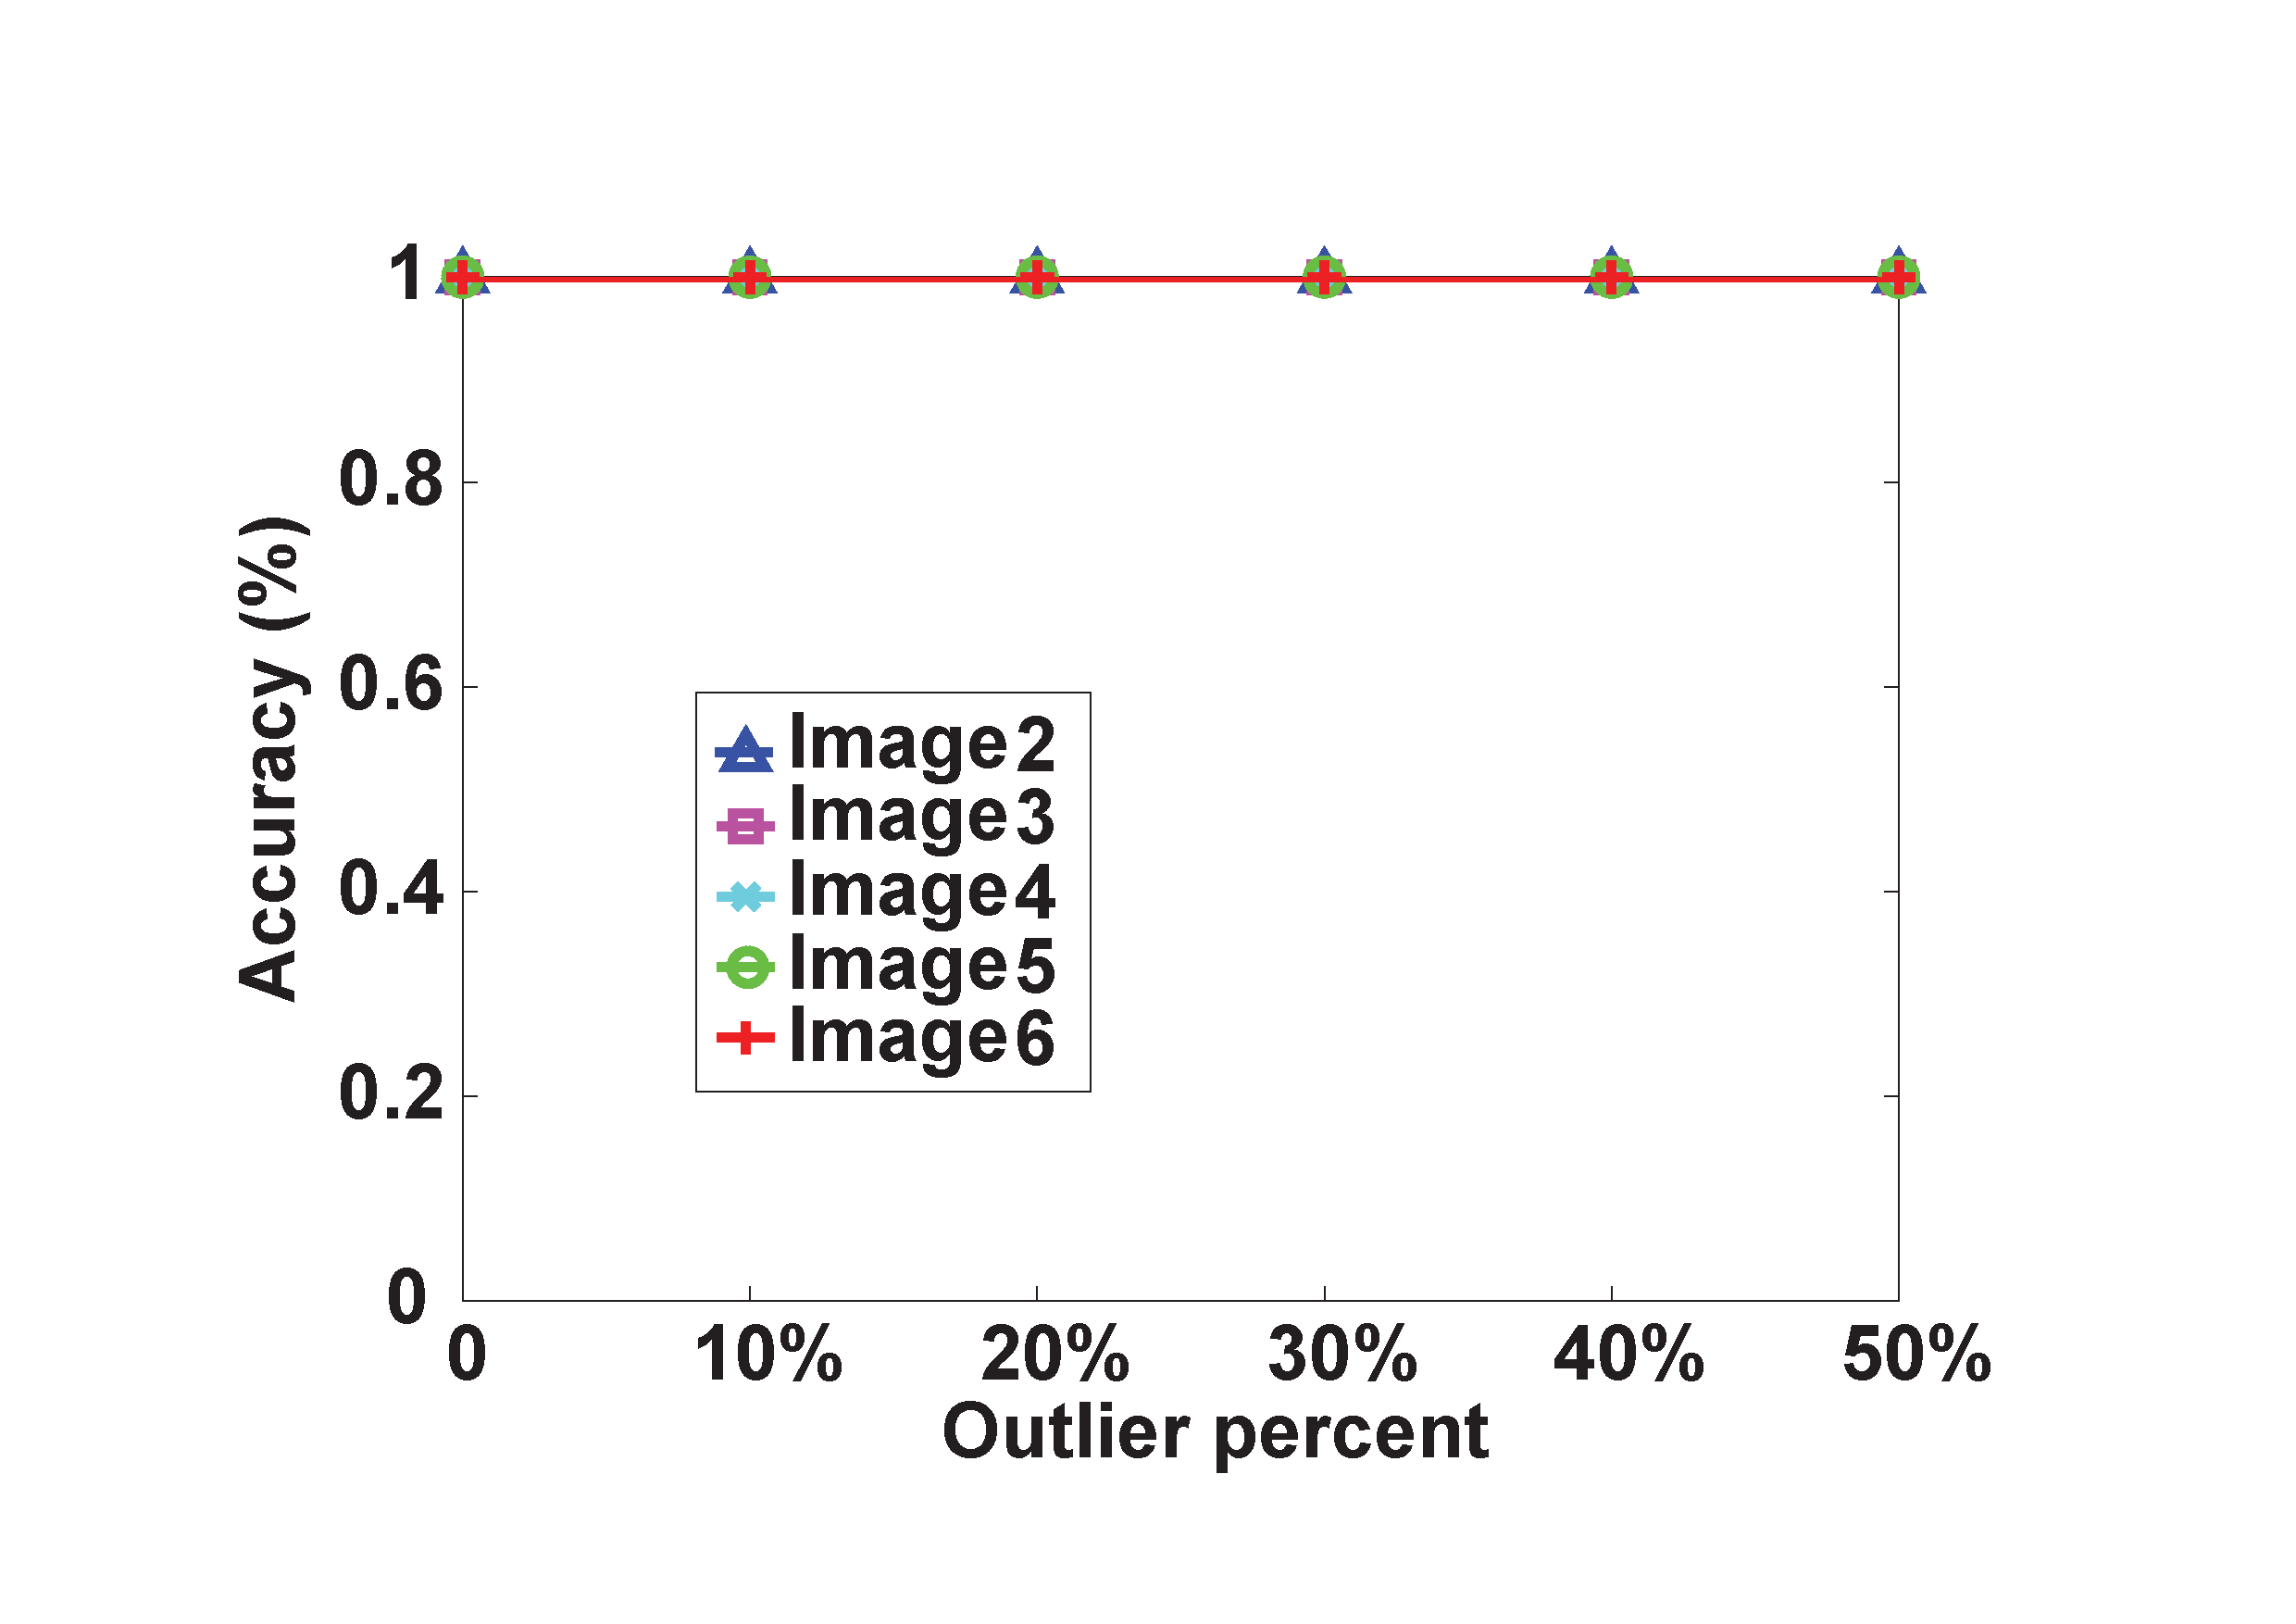
\includegraphics[width=58mm]{graf_OUR_ERRORRATE_embedded.pdf}%
            }%
        \end{minipage}%
        \hspace{10mm}%
        \addtocounter{subfigure}{-1}
        %----------------------------
        \begin{minipage}[b]{0.4\textwidth}
        \subfigure[]{
            \label{fig:subfig:wallerror4}
            \centering
            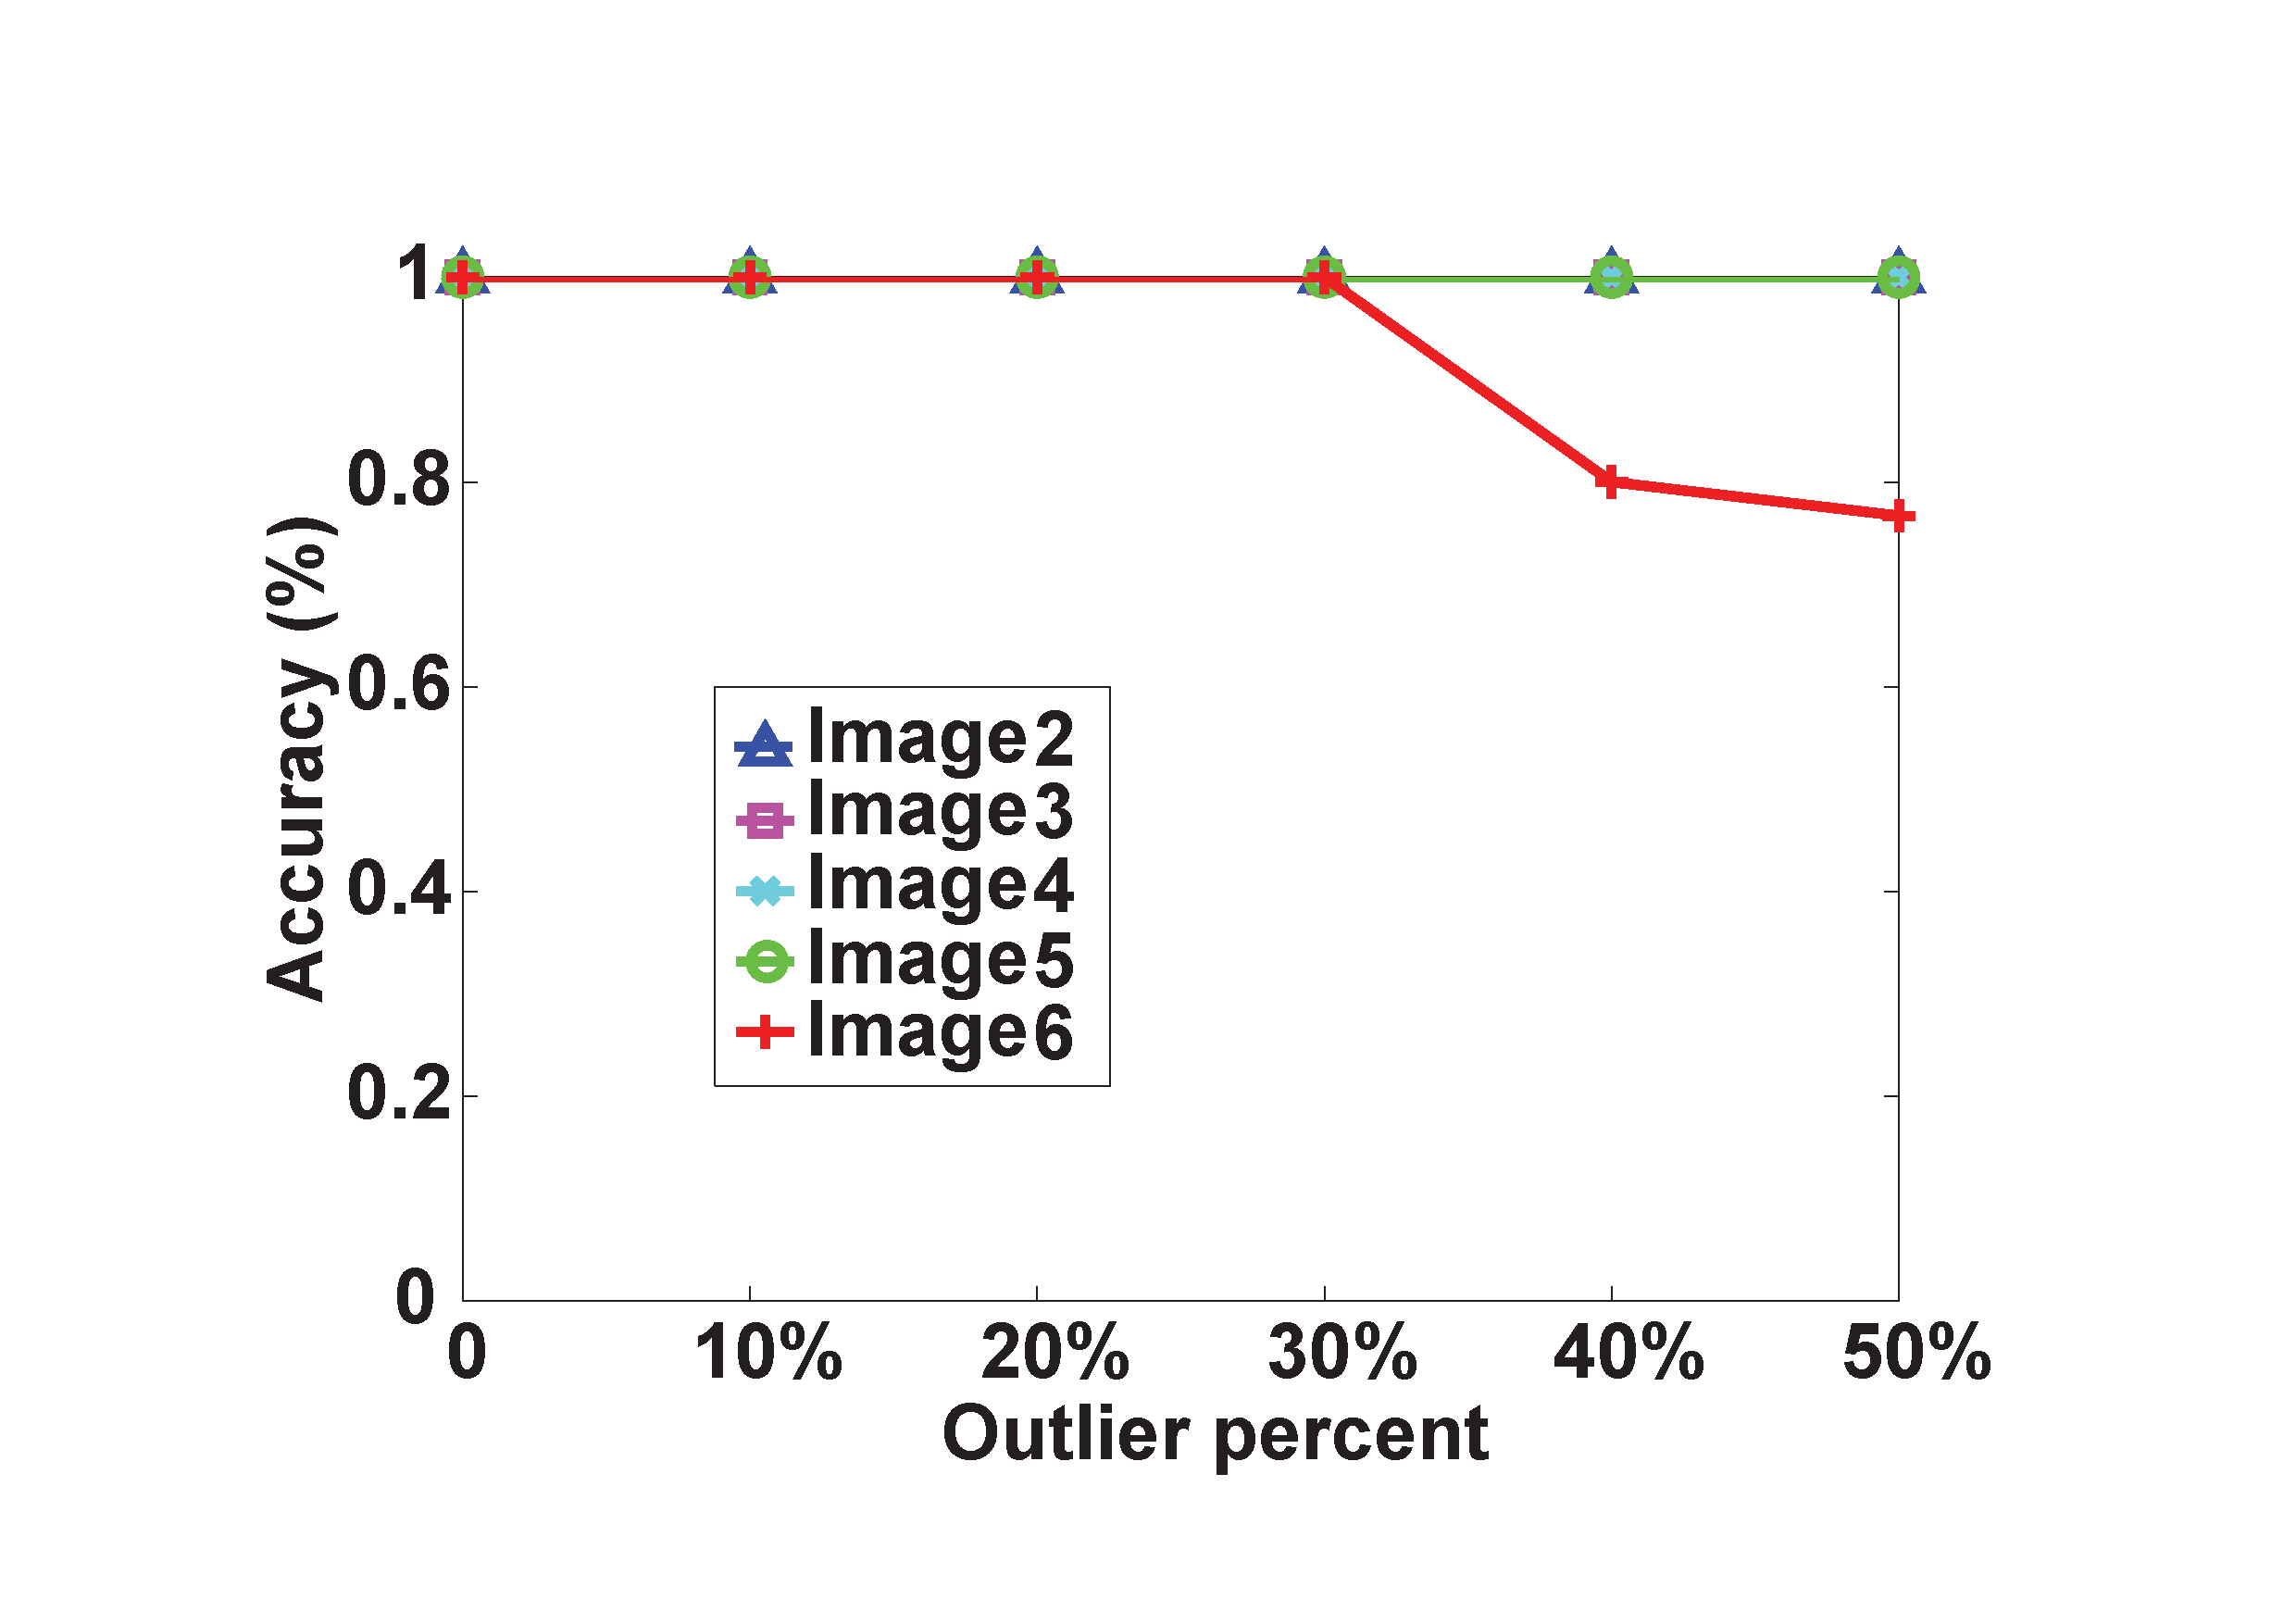
\includegraphics[width=58mm]{wall_OUR_ERRORRATE_embedded.pdf}%
            }%
        \end{minipage}%
        %\hspace{14mm}%
        \addtocounter{subfigure}{-1}
        \caption{Accuracy as a function of percentage of outliers. Left: \texttt{graf} set, right: \texttt{wall} set. Top to bottom: results for the spectral method~\cite{Cour06}, the hyper graph matching method~\cite{Zass08}, the tensor based method~\cite{Duchenne_etal09} and our method.}
\label{fig:mini:subfig_affineerrorrate} %% label for entire figure
%\vspace{-6mm}
\end{figure*}%
%
%------------------------------------------------
%  image matching results for both graf and wall
%------------------------------------------------
\begin{figure*}[!t]
%\vspace{-4mm}
%\hspace{-8ex}
\setlength{\abovecaptionskip}{0mm}
\setlength{\belowcaptionskip}{-2mm}
\centering
\setlength\subfigcapskip{-2mm}
\hspace{-8ex}
         %----------------------------
         %%% smac method
         %----------------------------
        \begin{minipage}[b]{0.4\textwidth}
        \subfigure{
            \label{fig:subfig:grafmatching1}
            \centering
            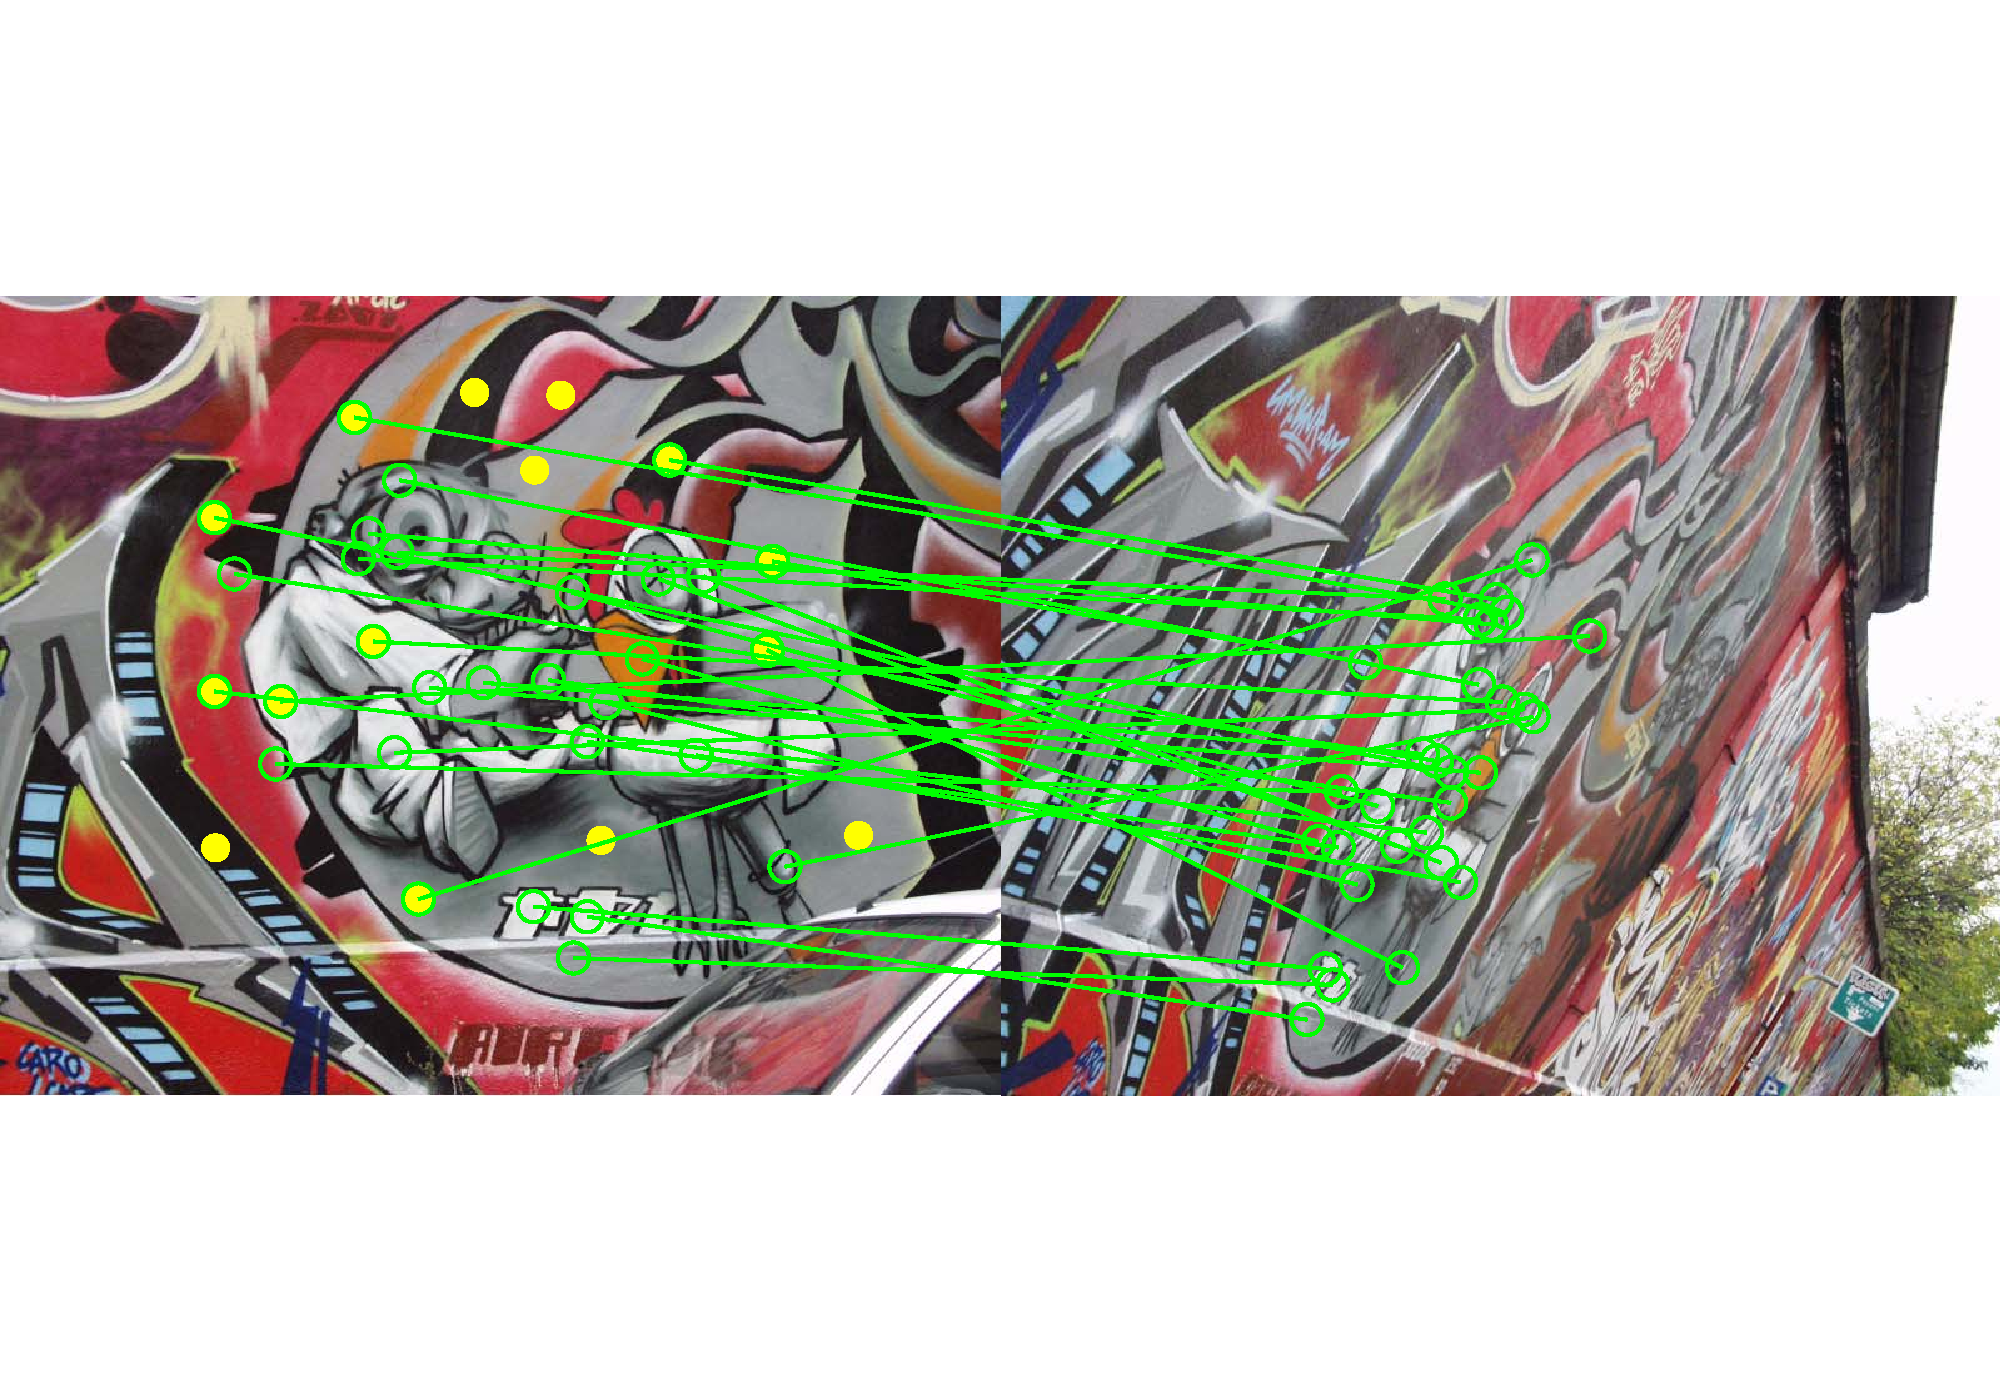
\includegraphics[width=62mm]{graf_SMAC_img6-50pNoise.pdf}%
            }%
        \end{minipage}%
        \hspace{10mm}%
        \addtocounter{subfigure}{-1}%
        %----------------------------
        \begin{minipage}[b]{0.4\textwidth}
        \subfigure{
            \label{fig:subfig:wallmatching1}
            \centering
            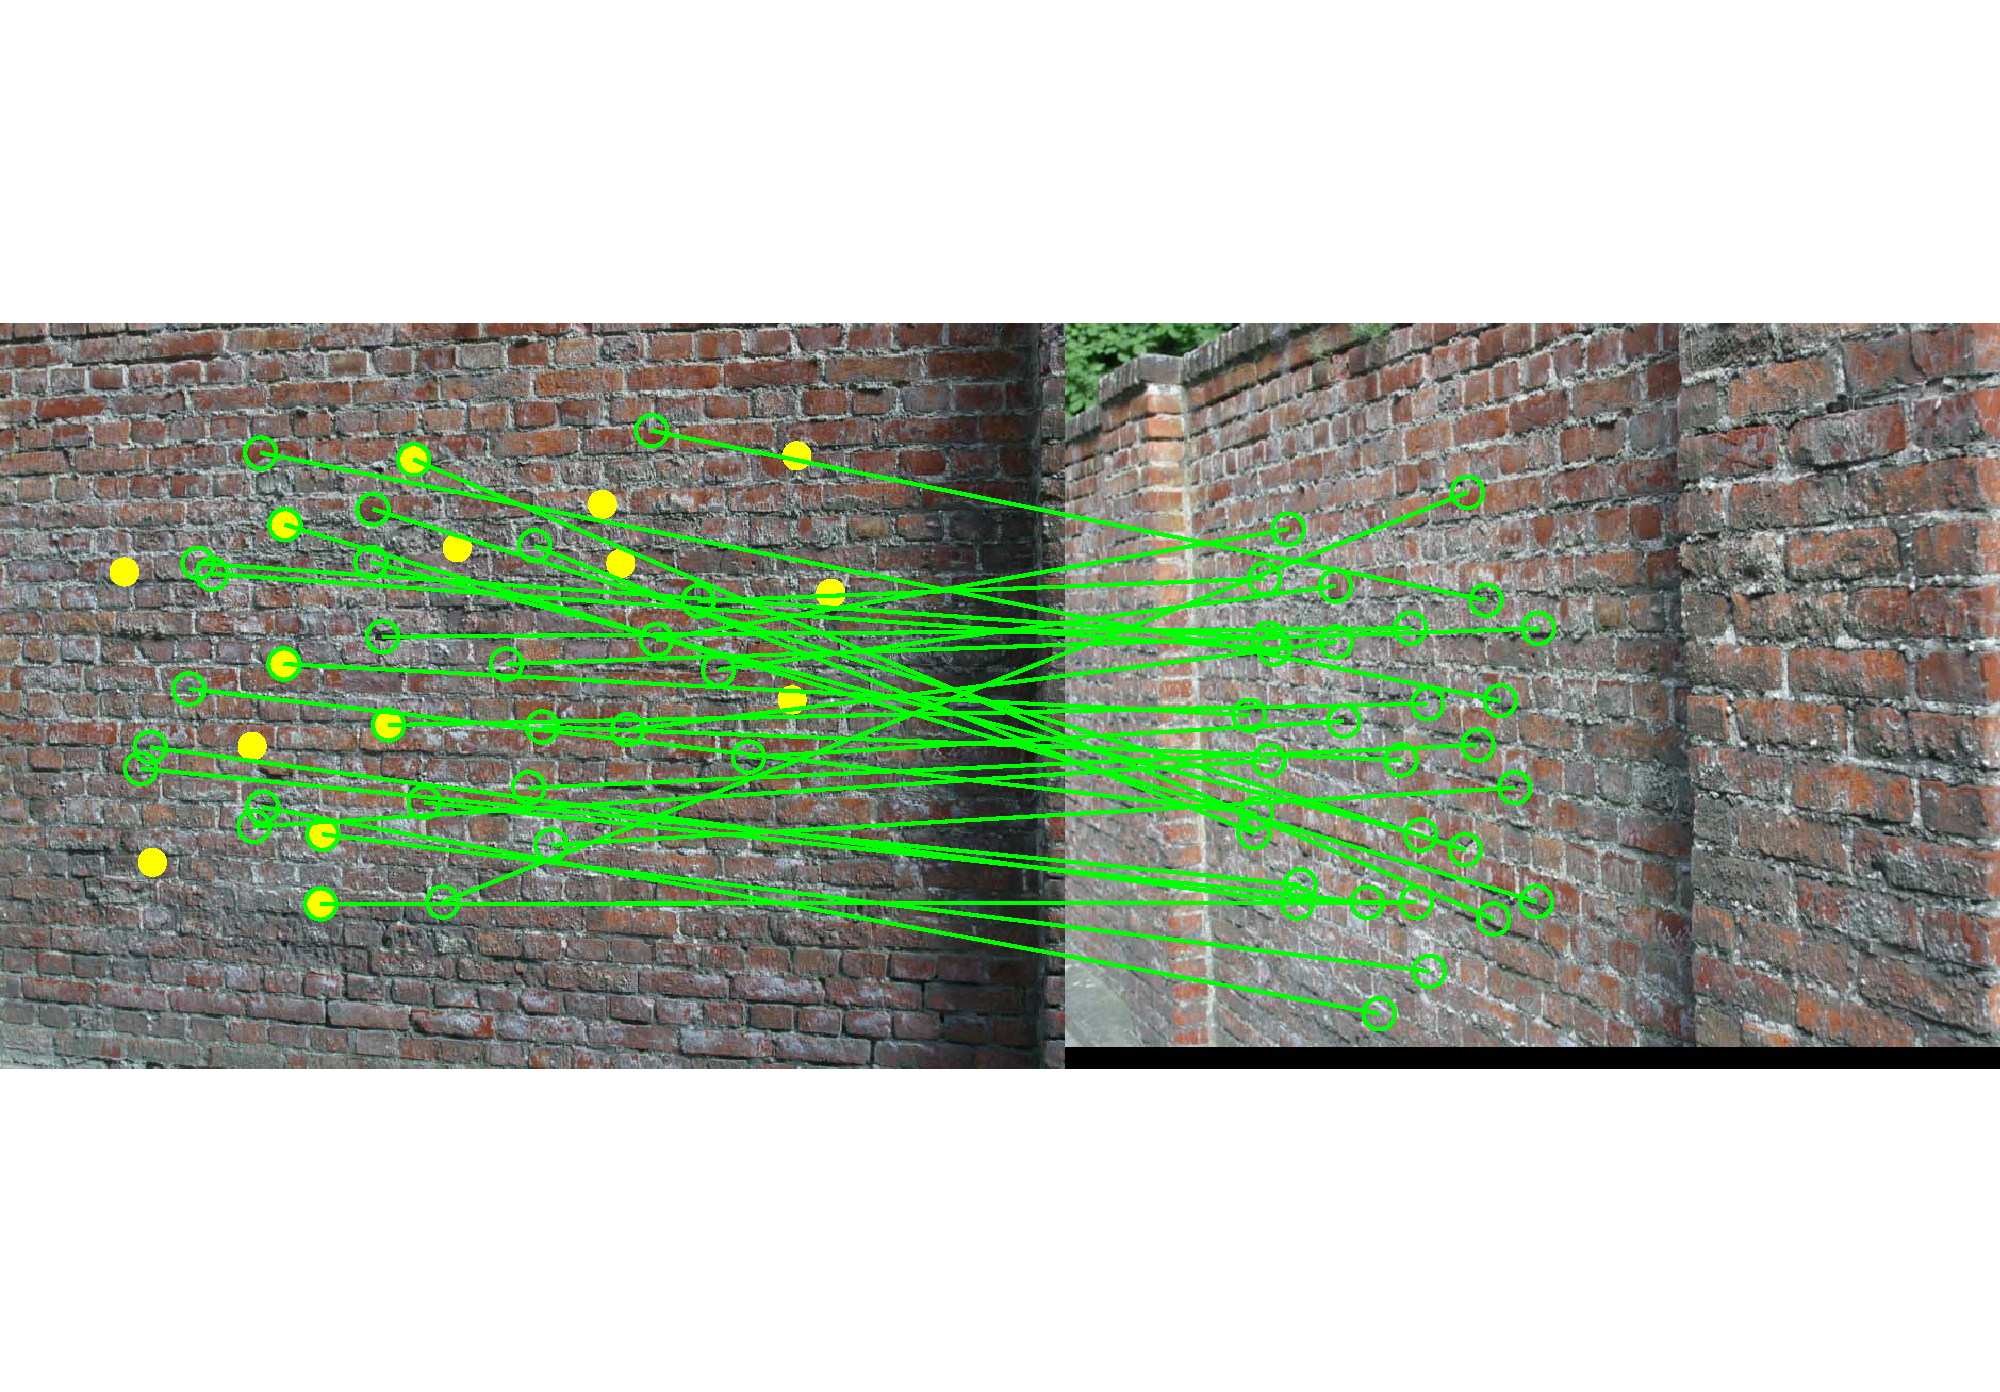
\includegraphics[width=66mm]{wall_SMAC_img6_50pNoise.pdf}%
            }%
        \end{minipage}\\%
        %\hspace{28mm}%
        \addtocounter{subfigure}{-1}%
        \hspace{-7ex}%
         %----------------------------
         %%% hyper method
         %----------------------------
        \begin{minipage}[b]{0.4\textwidth}
        \subfigure{
            \label{fig:subfig:grafmatching2}
            \centering
            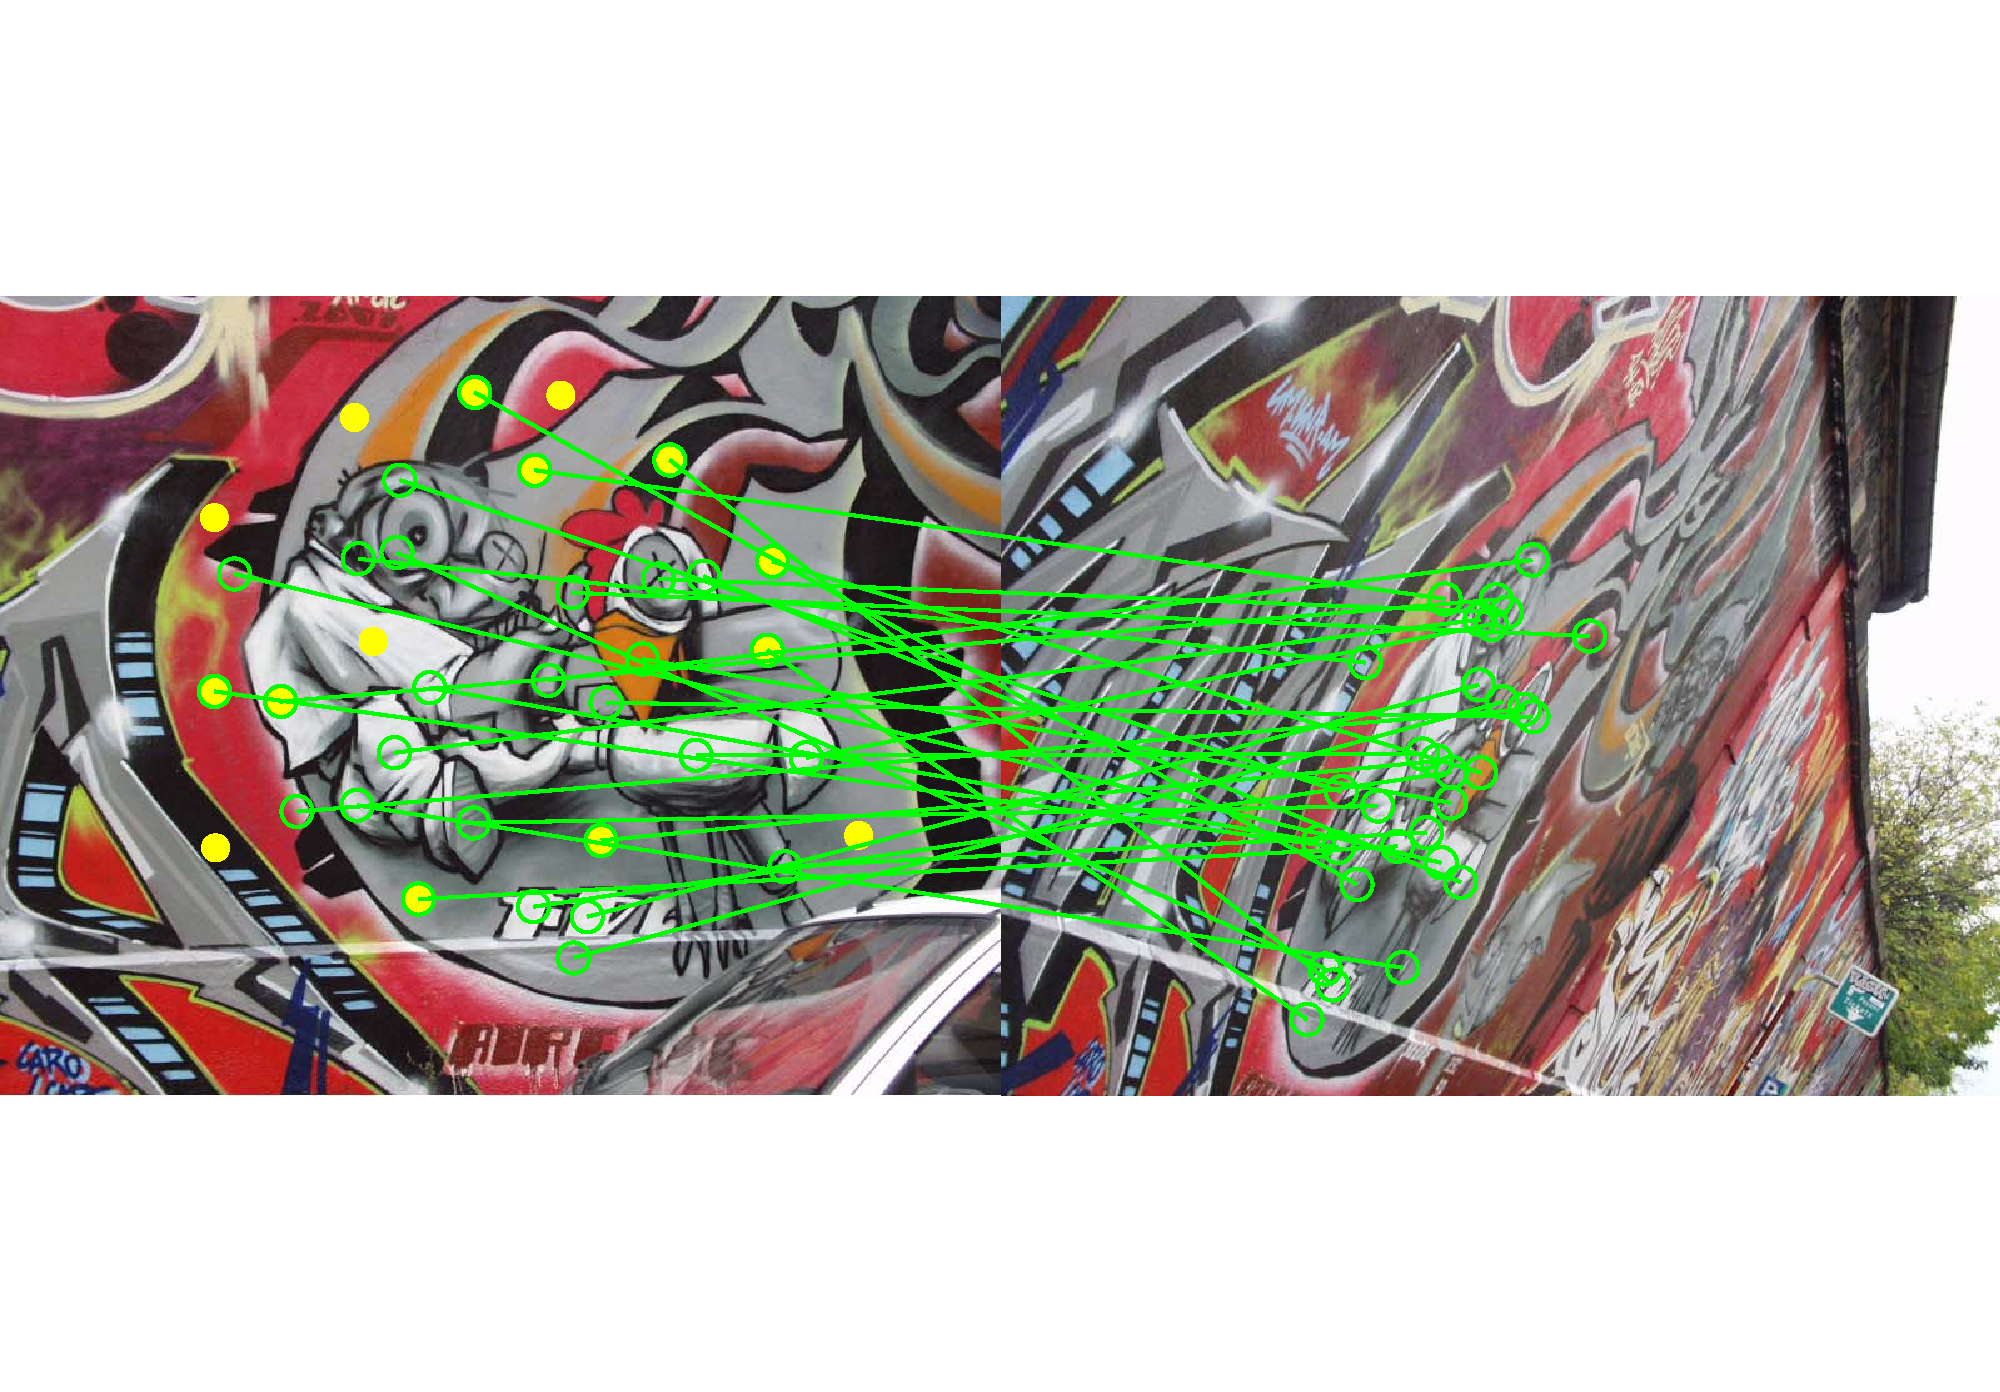
\includegraphics[width=62mm]{graf_HYPER_img6-50pNoise.pdf}%
            }%
        \end{minipage}%
        \hspace{10mm}%
        \addtocounter{subfigure}{-1}%
        %----------------------------
        \begin{minipage}[b]{0.4\textwidth}
        \subfigure{
            \label{fig:subfig:wallmatching2}
            \centering
            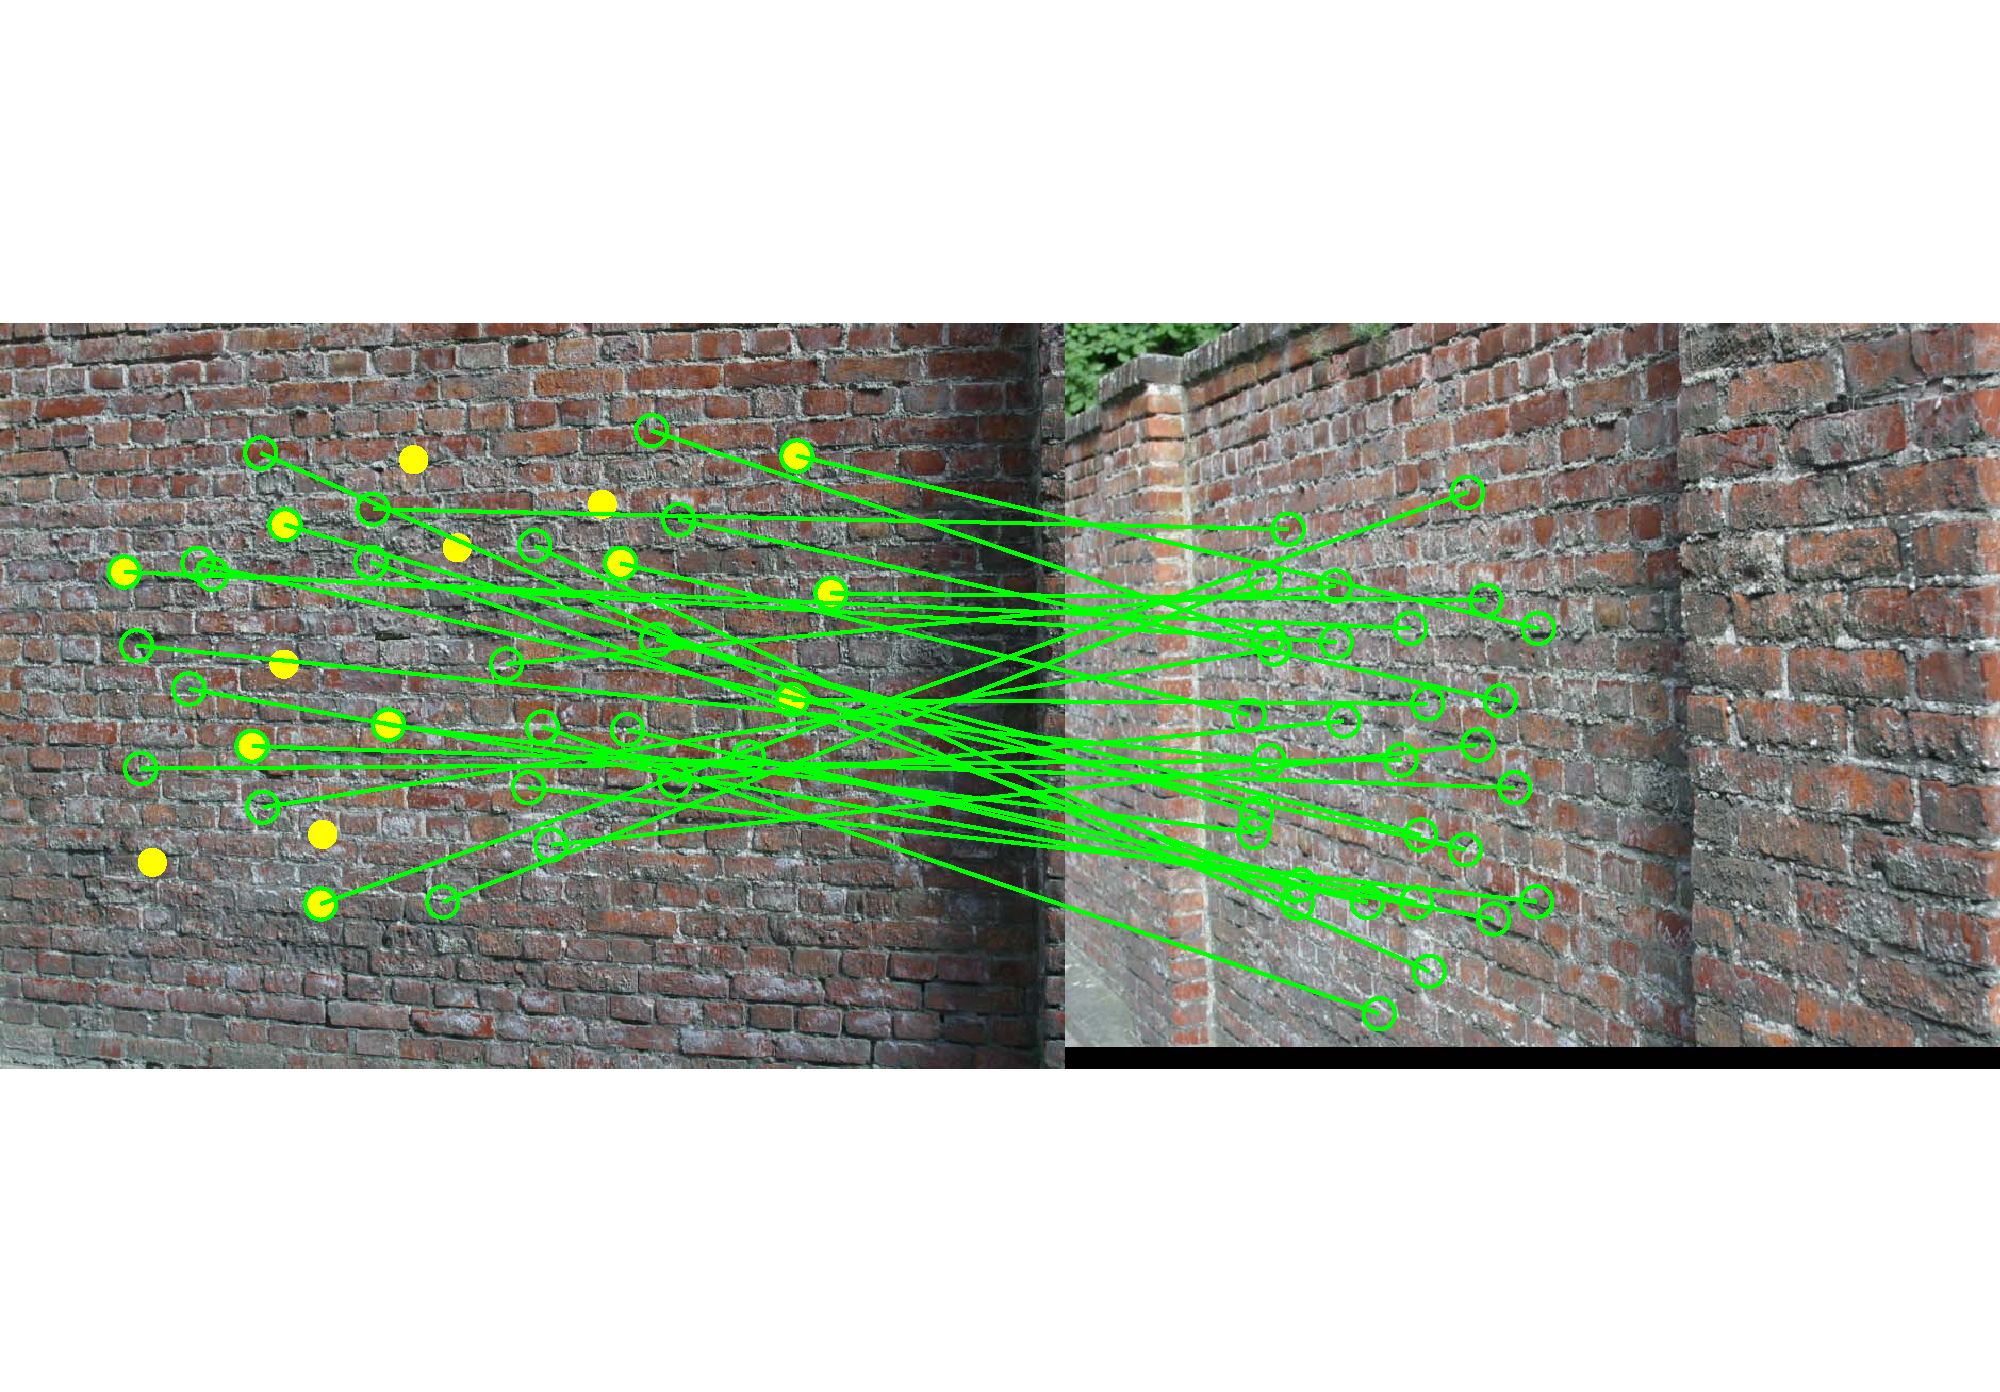
\includegraphics[width=66mm]{wall_HYPER_img6_50pNoise.pdf}%
            }%
        \end{minipage}\\%
        %\hspace{24mm}%
        \addtocounter{subfigure}{-1}%
        \hspace{-7ex}%
        %----------------------------
         %%% demo method
         %----------------------------
        \begin{minipage}[b]{0.4\textwidth}
        \subfigure{
            \label{fig:subfig:grafmatching3}
            \centering
            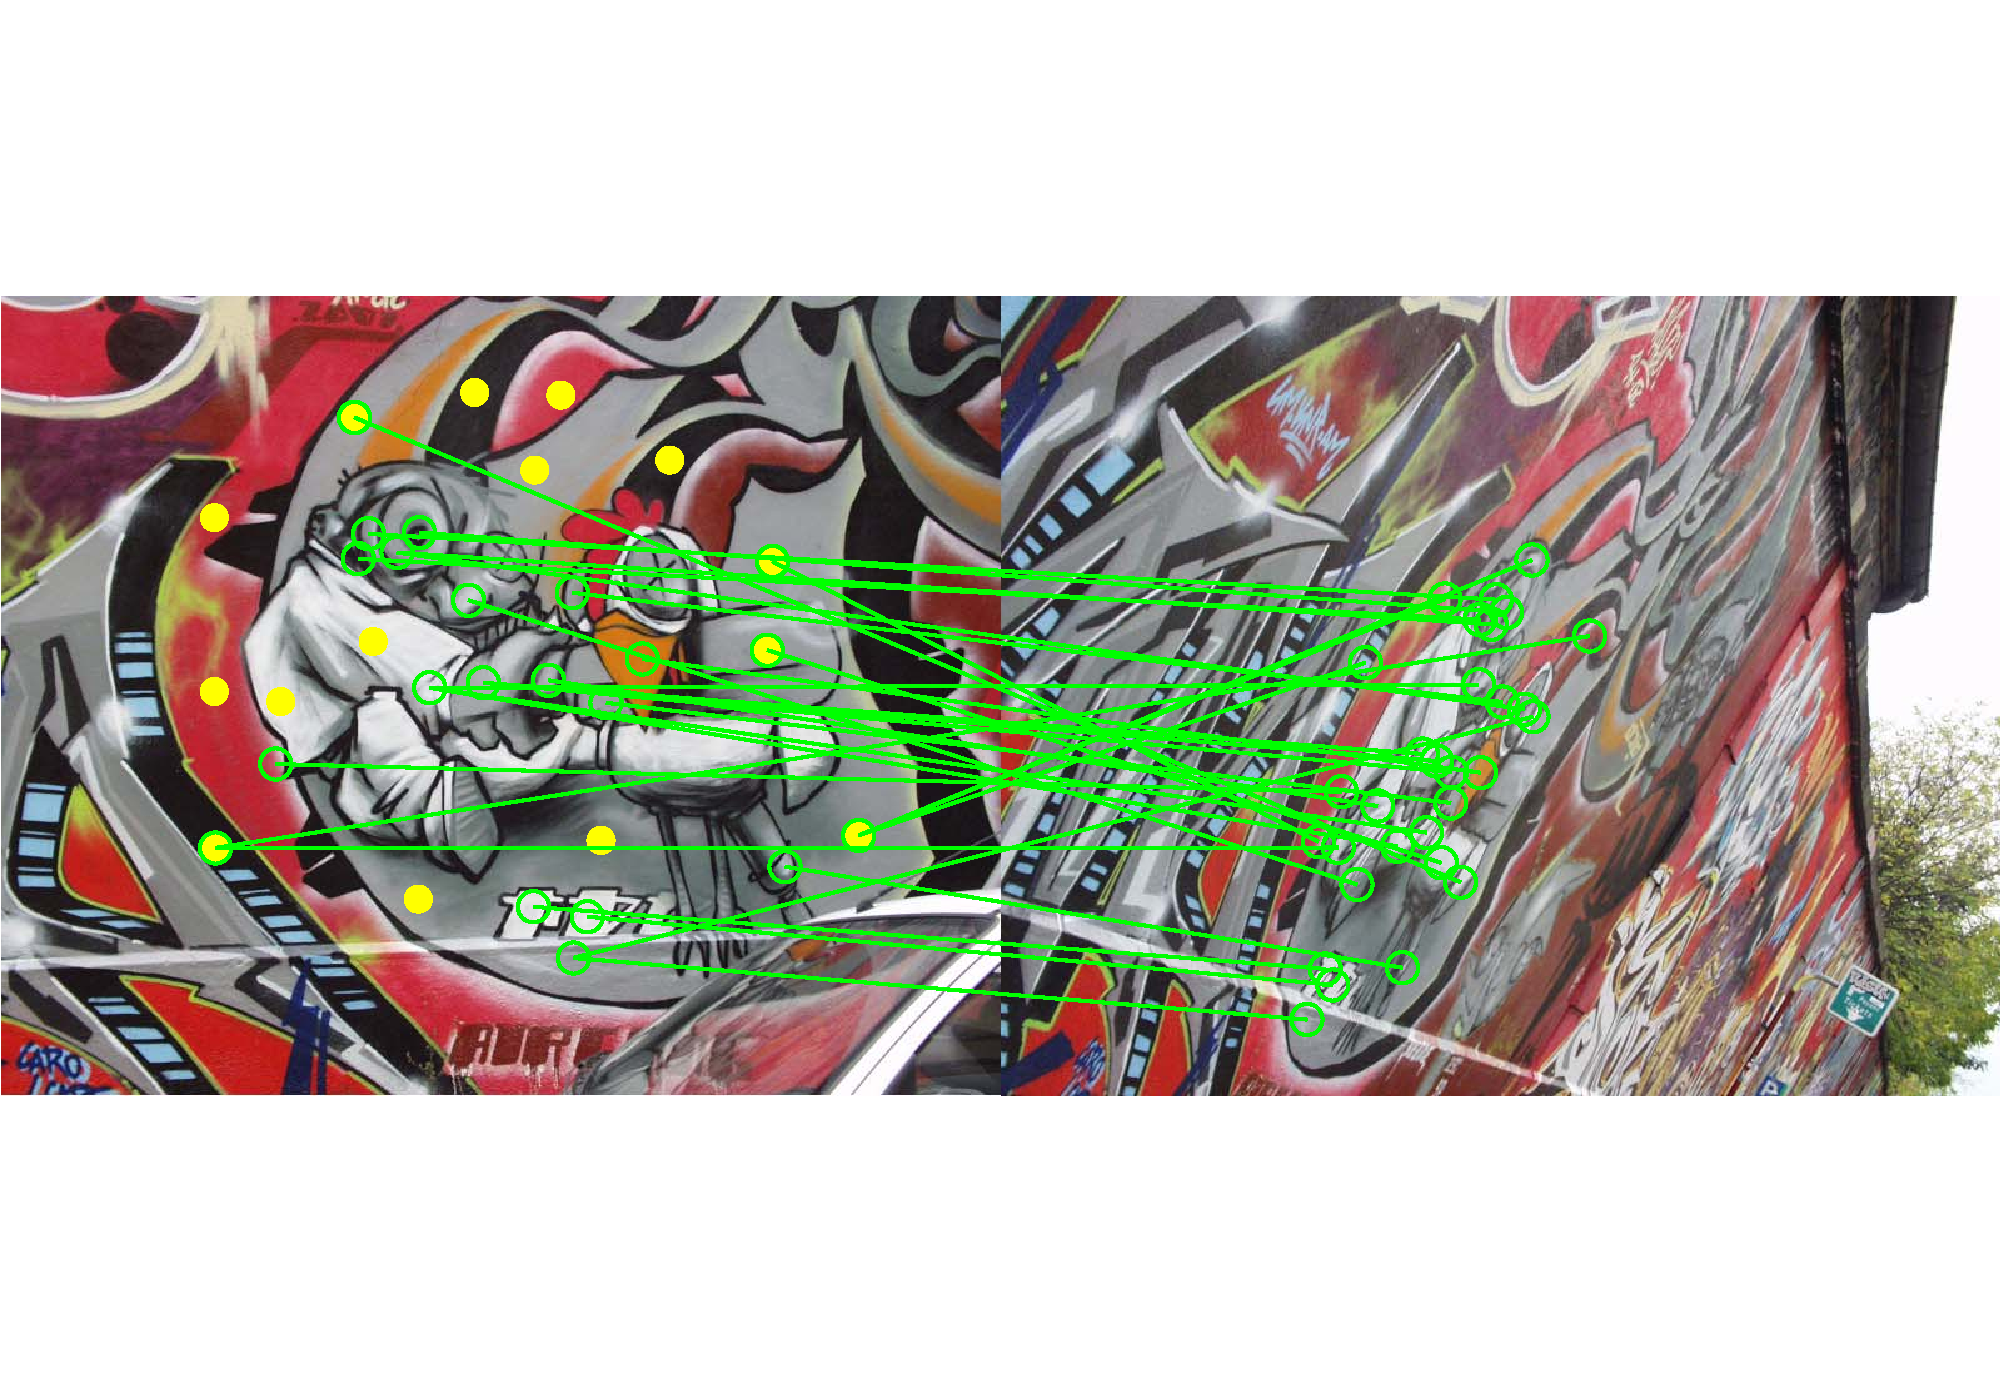
\includegraphics[width=62mm]{graf_DEMO_img6-50pNoise.pdf}%
            }%
        \end{minipage}%
        \hspace{10mm}%
        \addtocounter{subfigure}{-1}%
        %----------------------------
        \begin{minipage}[b]{0.4\textwidth}
        \subfigure{
            \label{fig:subfig:wallmatching3}
            \centering
            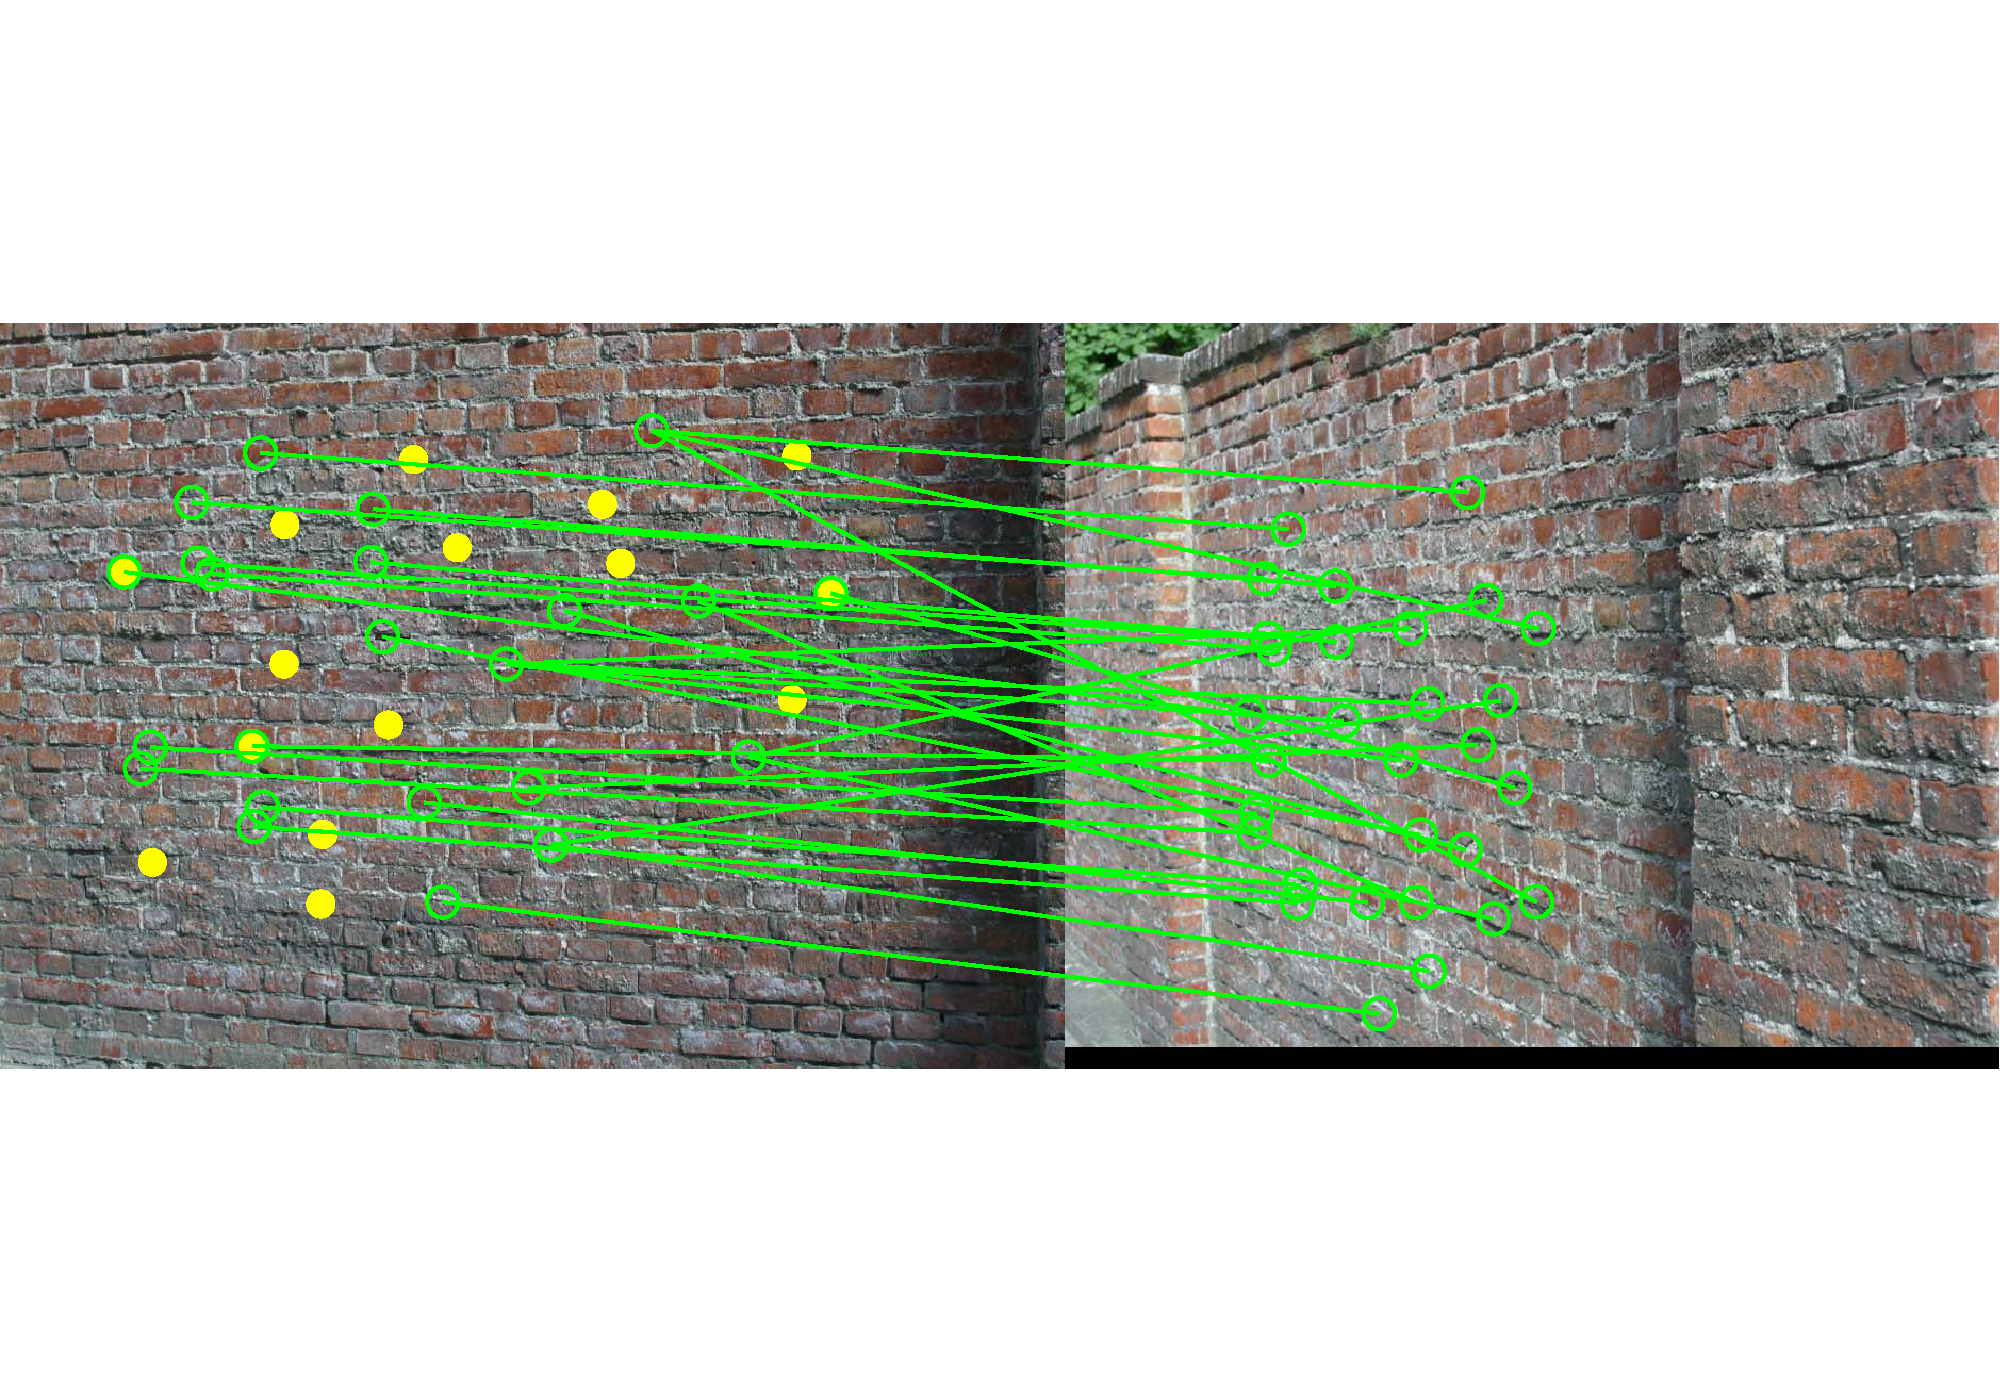
\includegraphics[width=66mm]{wall_DEMO_img6_50pNoise.pdf}%
            }%
        \end{minipage}\\%
        %\hspace{28mm}%
        \addtocounter{subfigure}{-1}%
        \hspace{-7ex}%
        %----------------------------
         %%% our method
         %----------------------------
        \begin{minipage}[b]{0.4\textwidth}
        \subfigure[]{
            \label{fig:subfig:grafmatching4}
            \centering
            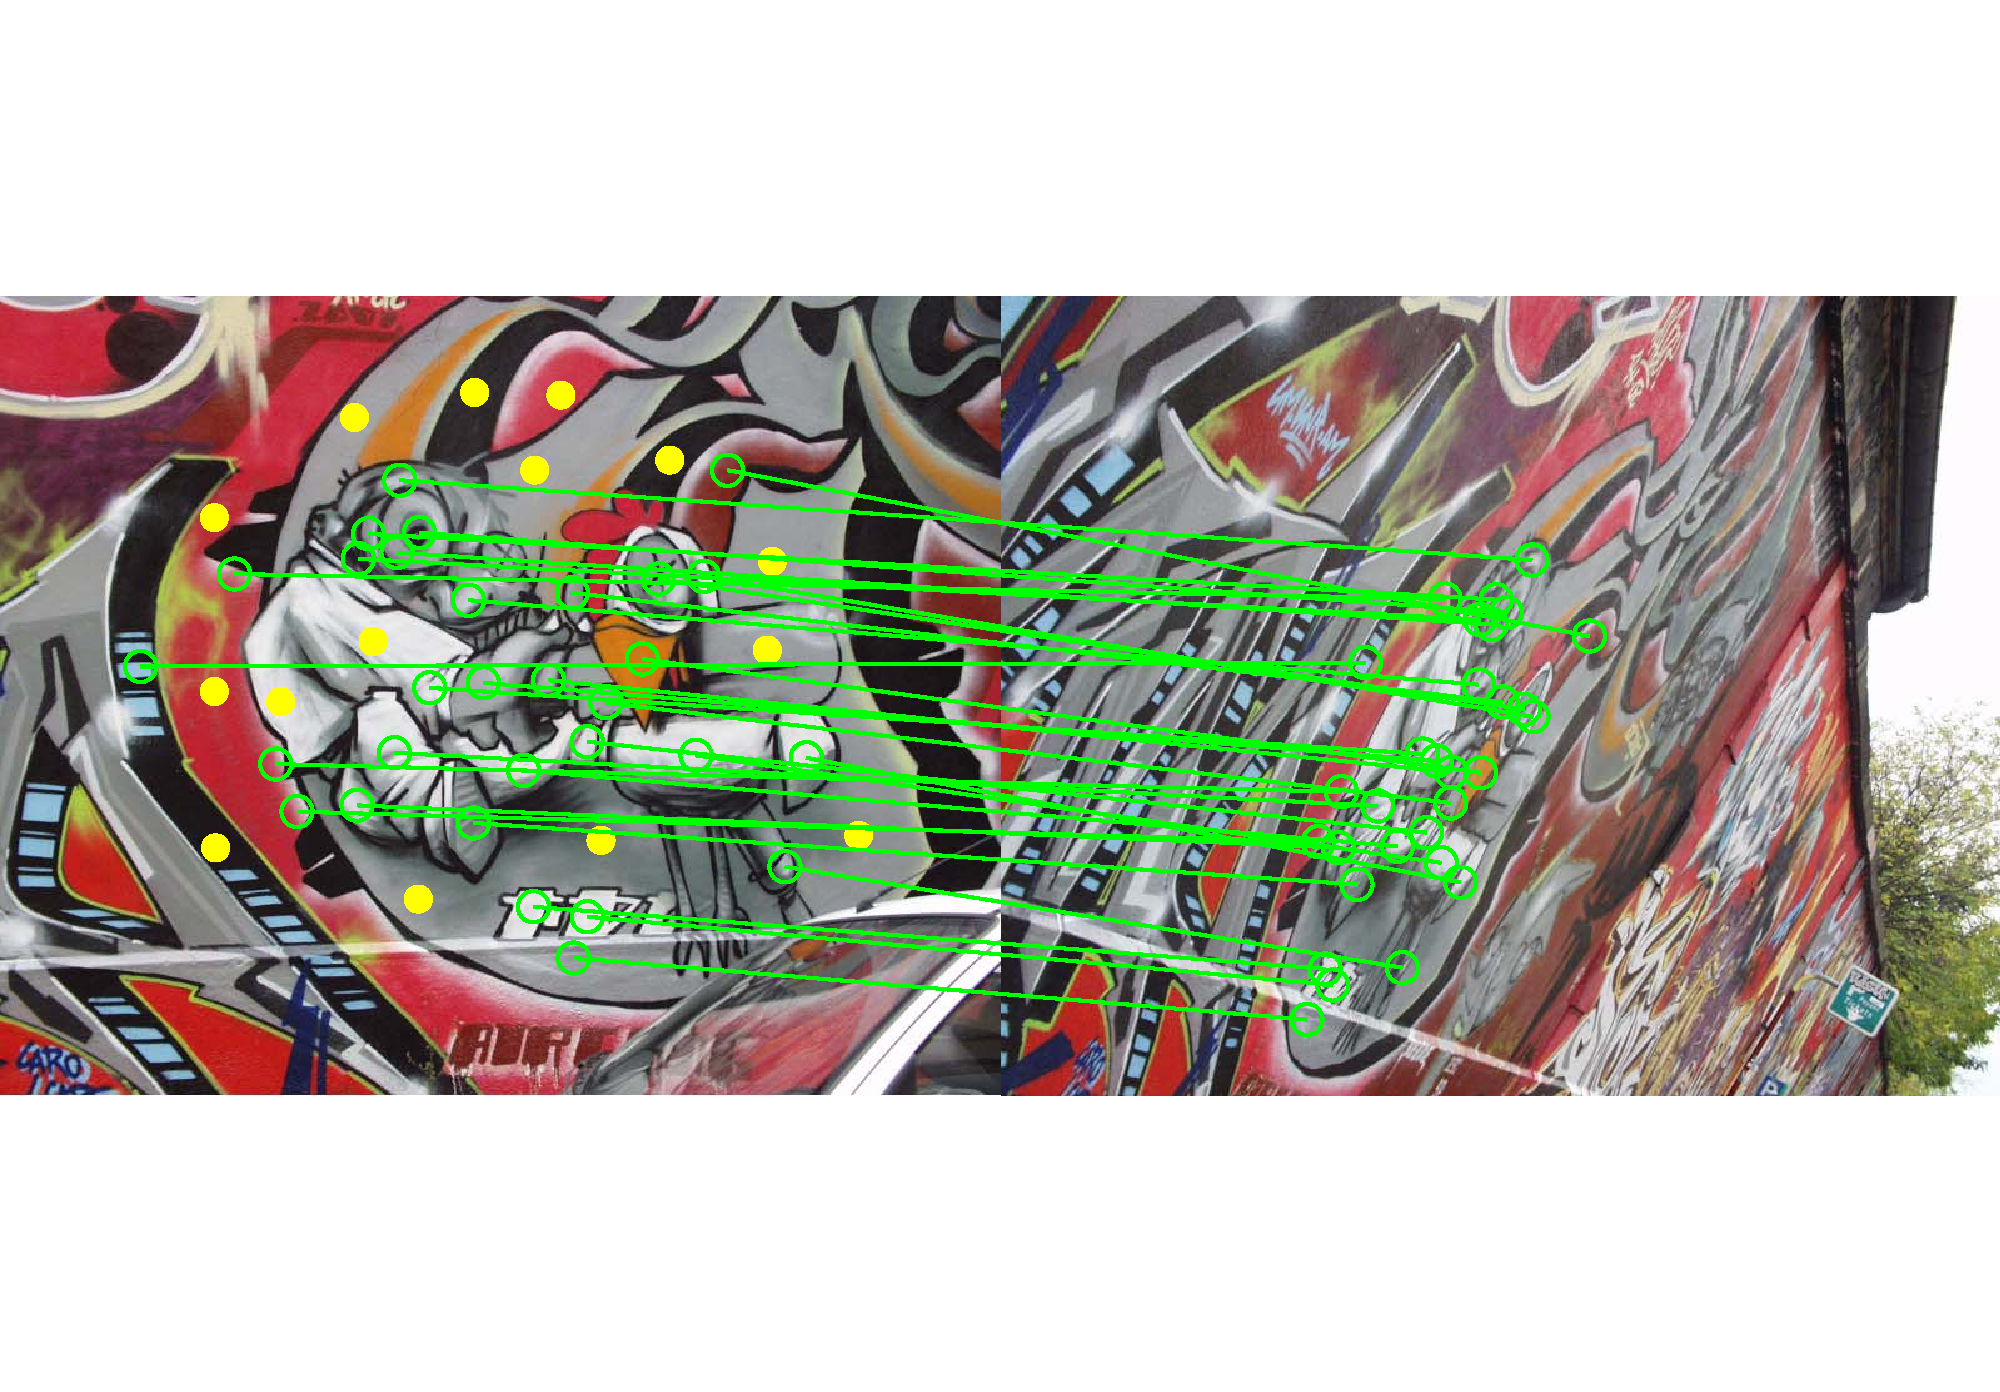
\includegraphics[width=62mm]{graf_our_img6-50pNoise.pdf}%
            }%
        \end{minipage}%
        \hspace{10mm}%
        %\addtocounter{subfigure}{-1}
        %----------------------------
        \begin{minipage}[b]{0.4\textwidth}
        \subfigure[]{
            \label{fig:subfig:wallmatching4}
            \centering
            \includegraphics[width=66mm]{wall_our_img6_50pNoise.pdf}%
            }%
        \end{minipage}%
        %\hspace{24mm}%
        %\addtocounter{subfigure}{-1}
        \caption{Matching images. Left: \texttt{graf} set, right: \texttt{wall} set. Top to bottom: results of the spectral method~\cite{Cour06}, the hypergraph matching method~\cite{Zass08}, the tensor based method~\cite{Duchenne_etal09} and our method. The feature set $P_1$ contains $50\%$ outliers. }
\label{fig:mini:subfig_affinematchingimages} %% label for entire figure
\end{figure*}%

In both image sets, the images were taken from quite different viewpoints, leading to quite different texture appearances. It is thus difficult to match features just using an MSER detector or a SIFT detector.
The results in Fig.\ref{fig:mini:subfig_affineerrorrate} show that the pairwise method SMAC~\cite{Cour06} as a result fails to provide a high matching accuracy, while the higher-order methods are much better as they take structural information
into account. They work well if there are not too many outliers.

It is clear that our method is much more stable than the other higher-order methods. For the \texttt{graf} image set our method correctly matched the feature set $P_1$ to $P_2$ in images 2--6 up to the maximum outlier percentage. For image 6 of the \texttt{wall} set, our method still found most correct correspondences with $33.3\%$ outliers. Although the tensor based method and the hyper graph matching method~\cite{Zass08} performed well in the absence of outliers, their matching accuracy dropped rapidly as the outlier percentage increased.

%-------------------------------------------------------------------------
\subsection{Deformable surface matching}
\label{subsec:deformabledata}

Registration of an object subject to large non-affine deformations is also an important problem. To assess the performance of our method, we established correspondences of feature points on the surface of a deforming object using our method, the spectral method~\cite{Cour06}, the tensor based method~\cite{Duchenne_etal09} and the hyper graph matching method~\cite{Zass08}. Again, all higher-order methods used the same third-order potentials from Section~\ref{sec:implementation} and all maintained an equivalent tensor size.

We chose four deformable surface image sets\footnote{From \url{http://cvlab.epfl.ch/data/dsr/}} containing a cloth, a curving piece of paper, a cushion and a creasing piece of paper. The surfaces of the cloth and the curving piece of paper underwent relatively smooth deformations, while the surfaces of the cushion and the creasing piece of paper included sharp folds.

From each image set we randomly chose six frames before and after a large deformation. We randomly chose $100$ corresponding points on each surface to be the features, using the provided ground truth.
In each image set we chose the features on the frame most unlike the others  (shown in Fig.\ref{fig:mini:subfig_deformableimages}) as $P_1$ and matched them with the features in the other five frames.
%----------------------------------------
%  deformable matching : model features
%----------------------------------------
\begin{figure*}[!t]
%\vspace{-4mm}
%\hspace{-8ex}
%\setlength{\abovecaptionskip}{2mm}
%\setlength{\belowcaptionskip}{2mm}
\renewcommand\thesubfigure{}
\centering
\setlength\subfigcapskip{-4mm}
%\vspace{-2ex}
        \hspace{-8ex}
        \begin{minipage}[b]{0.2\textwidth}
            \subfigure[\scriptsize Frame 299]{
            \label{fig:subfig:cloth1}
            \centering
            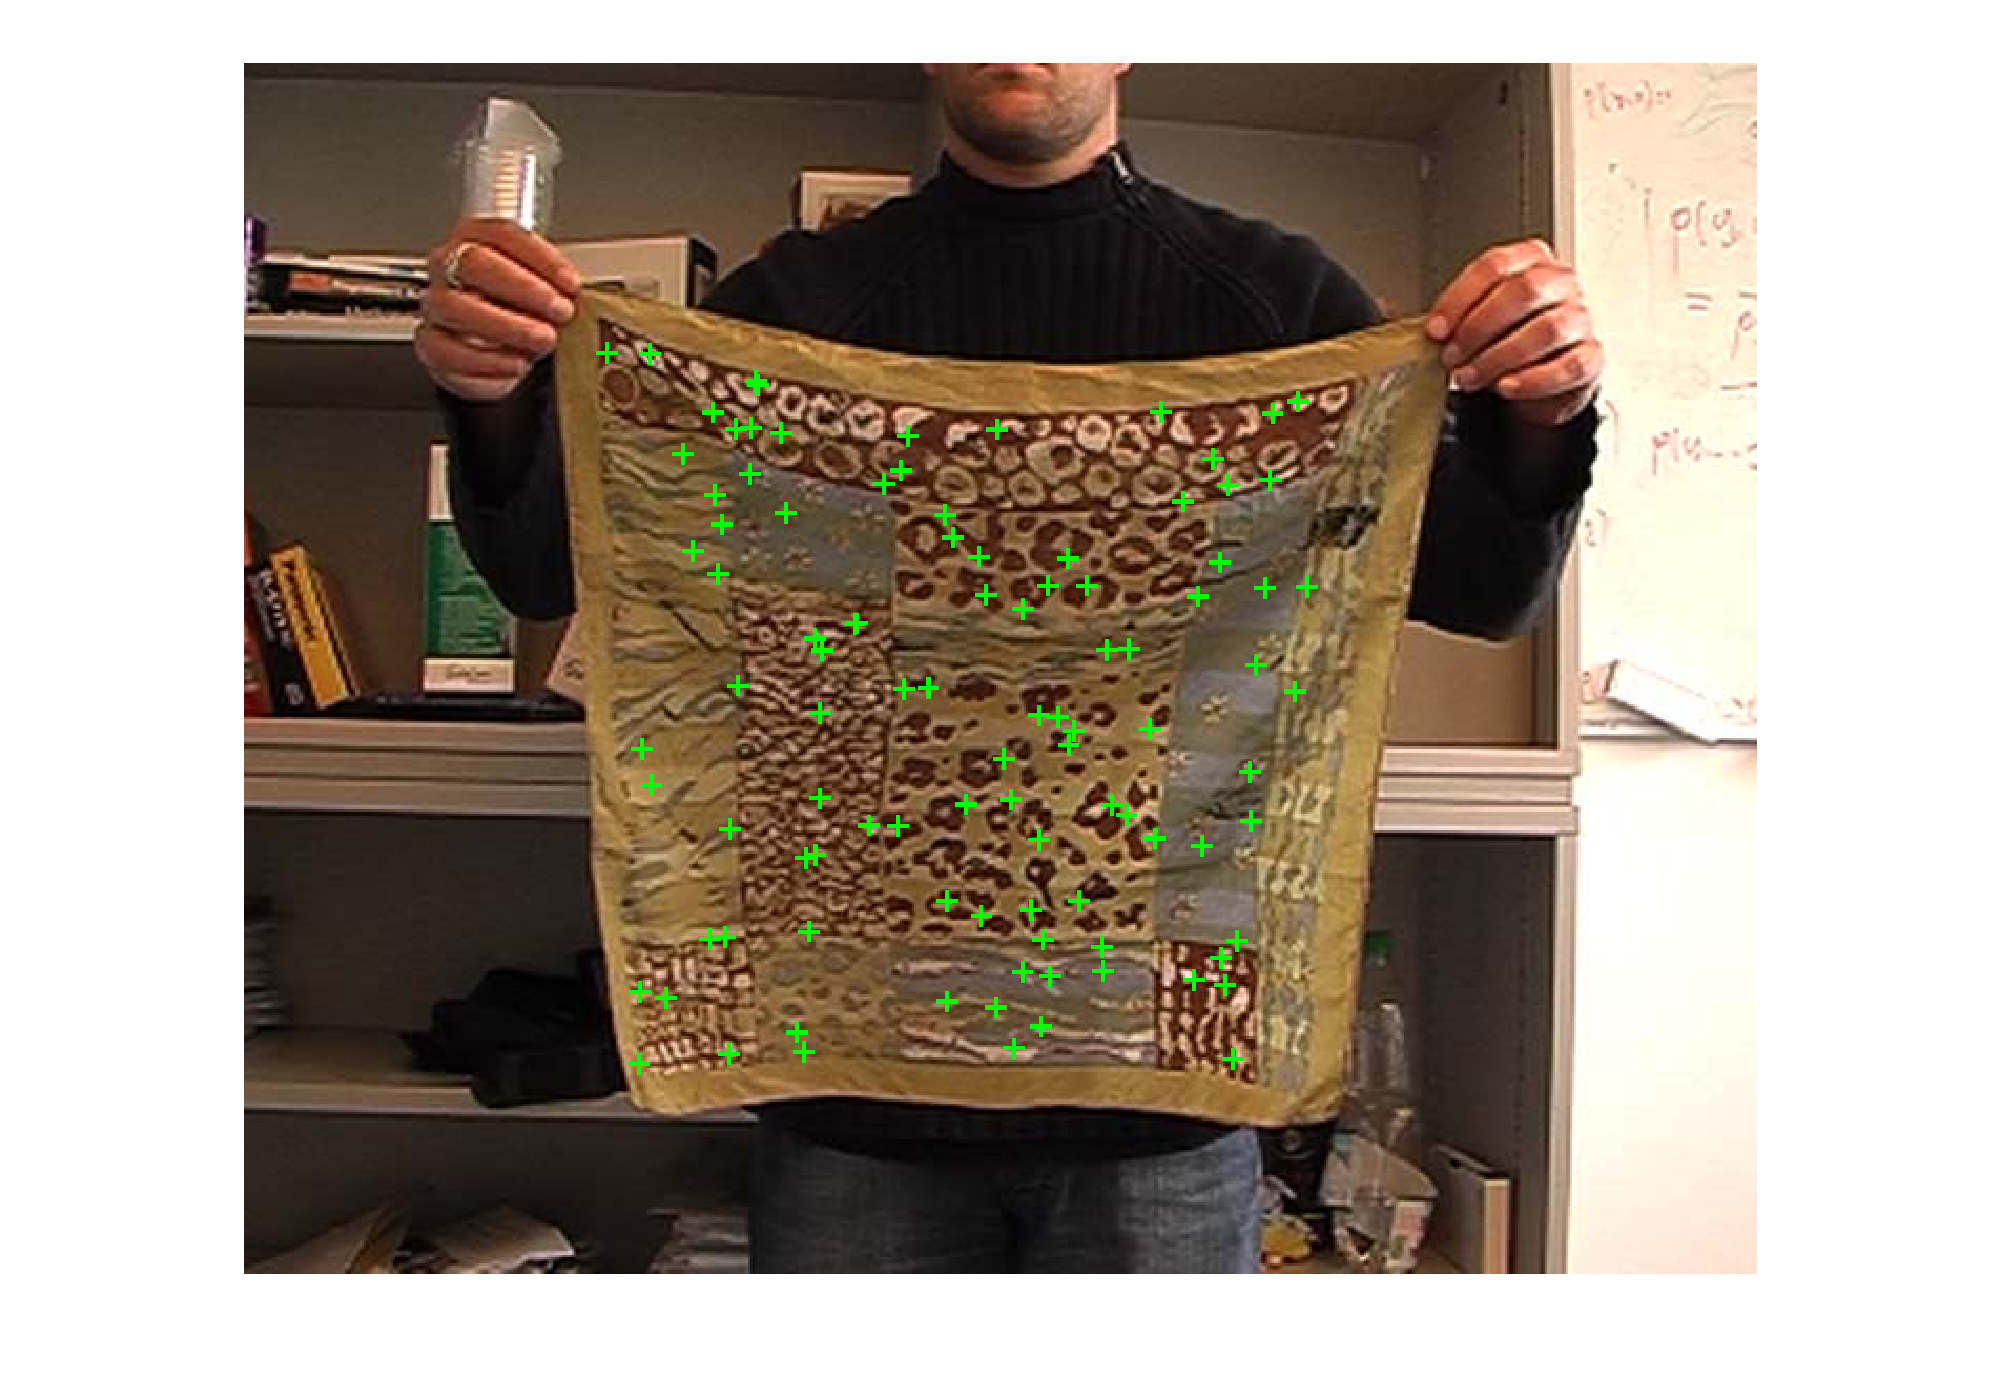
\includegraphics[width=36mm]{cloth_299.pdf}}%
        \end{minipage}%
        \hspace{5mm}%
        \addtocounter{subfigure}{-1}
        %%%
        \begin{minipage}[b]{0.2\textwidth}
            \subfigure[\scriptsize Frame 314]{
            \label{fig:subfig:paperB1}
            \centering
            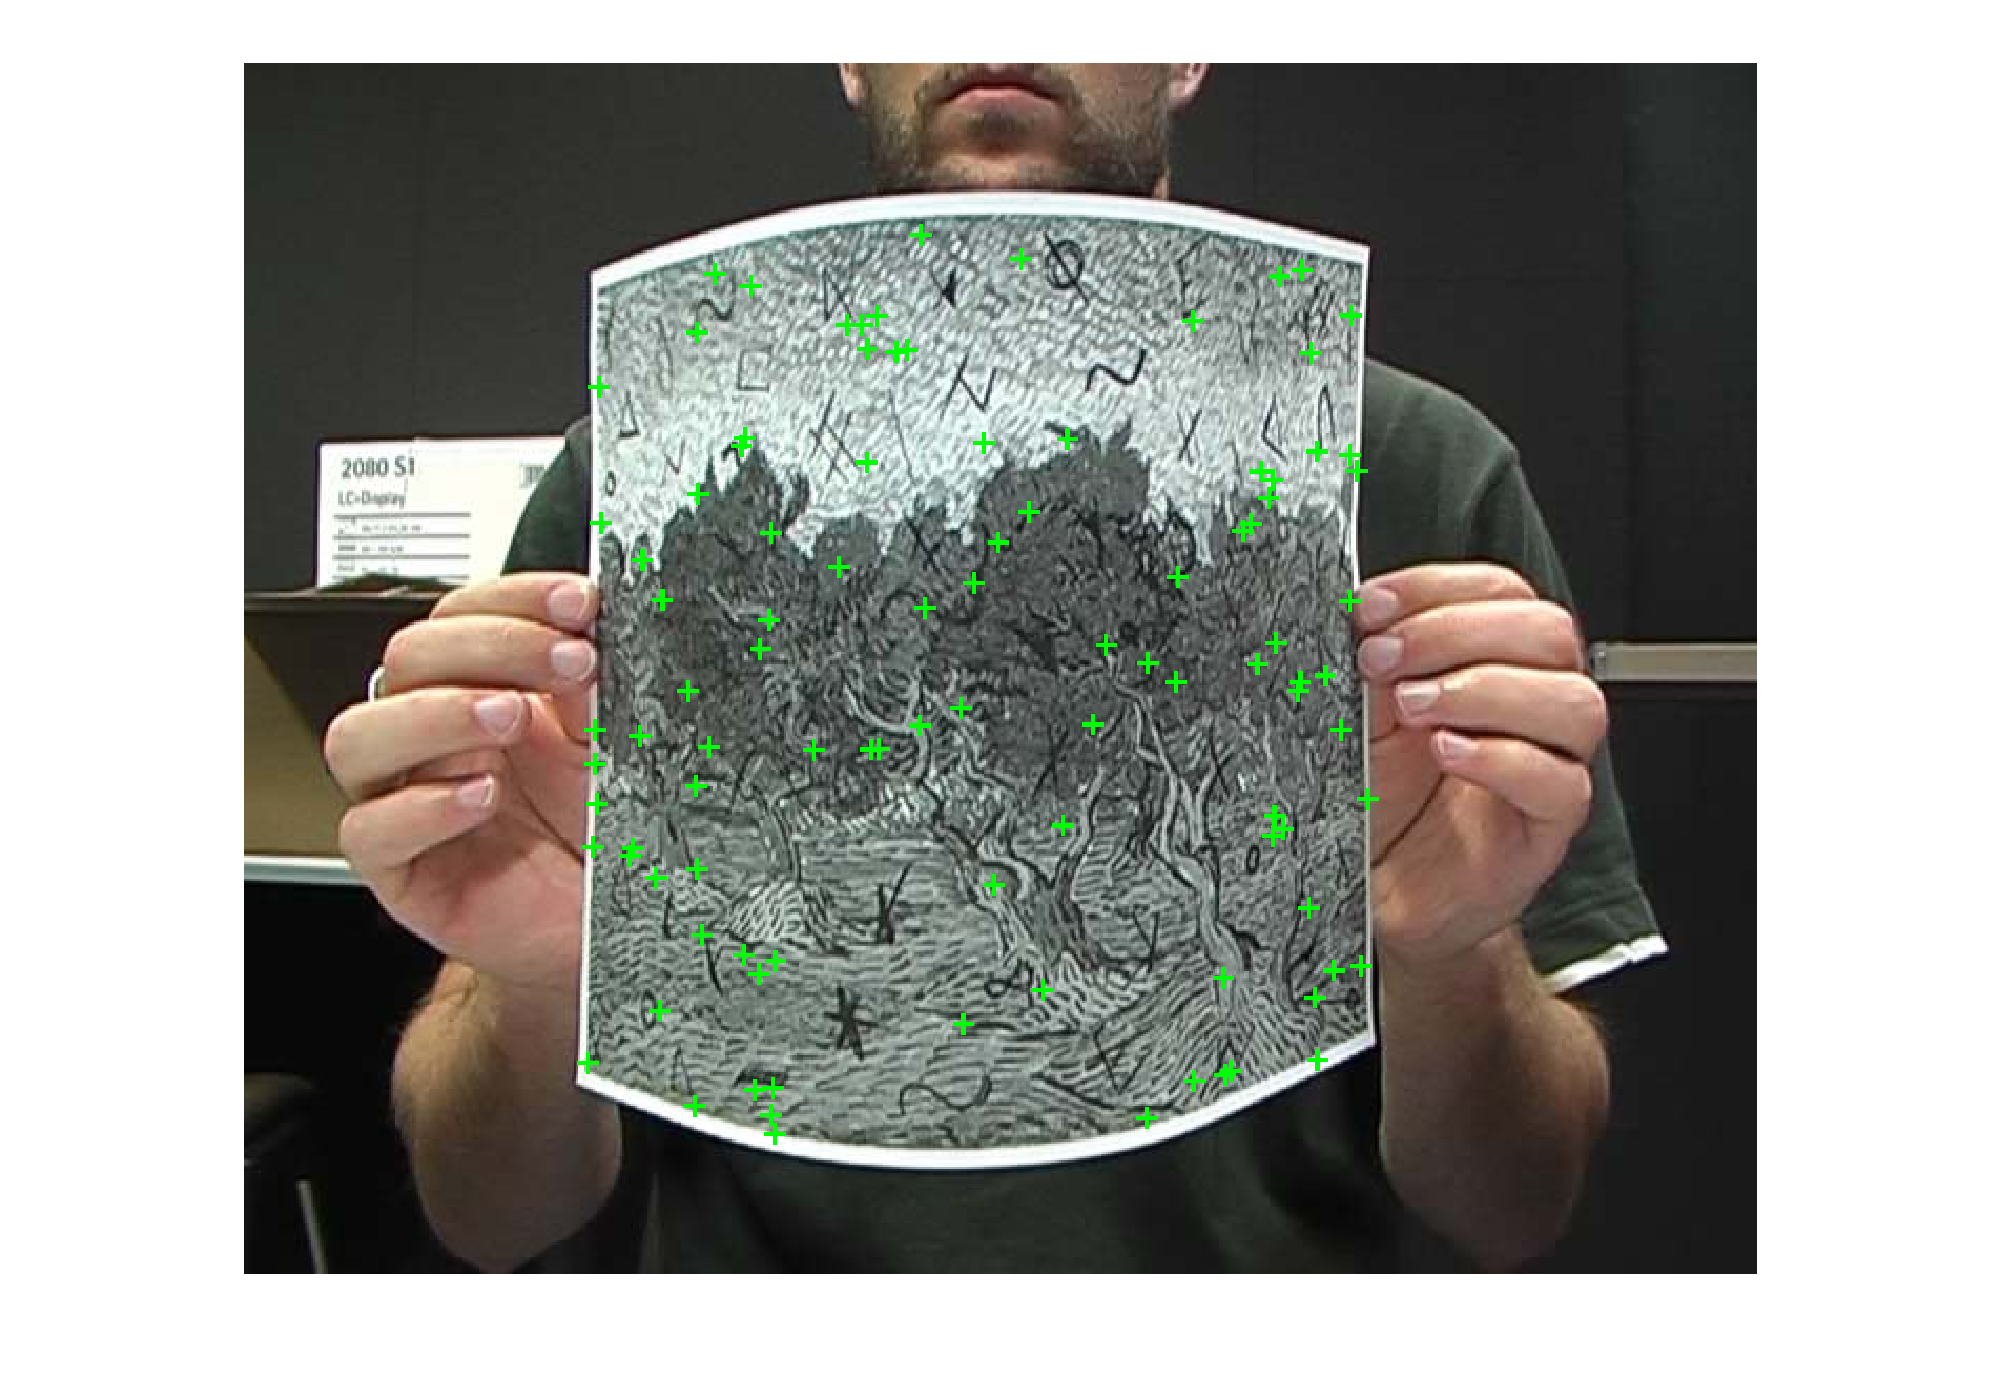
\includegraphics[width=36mm]{paperB_314.pdf}}%
        \end{minipage}%
        \hspace{5mm}%
        \addtocounter{subfigure}{-1}
        %%%
        \begin{minipage}[b]{0.2\textwidth}
            \subfigure[\scriptsize Frame 213]{
            \label{fig:subfig:cushion1}
            \centering
            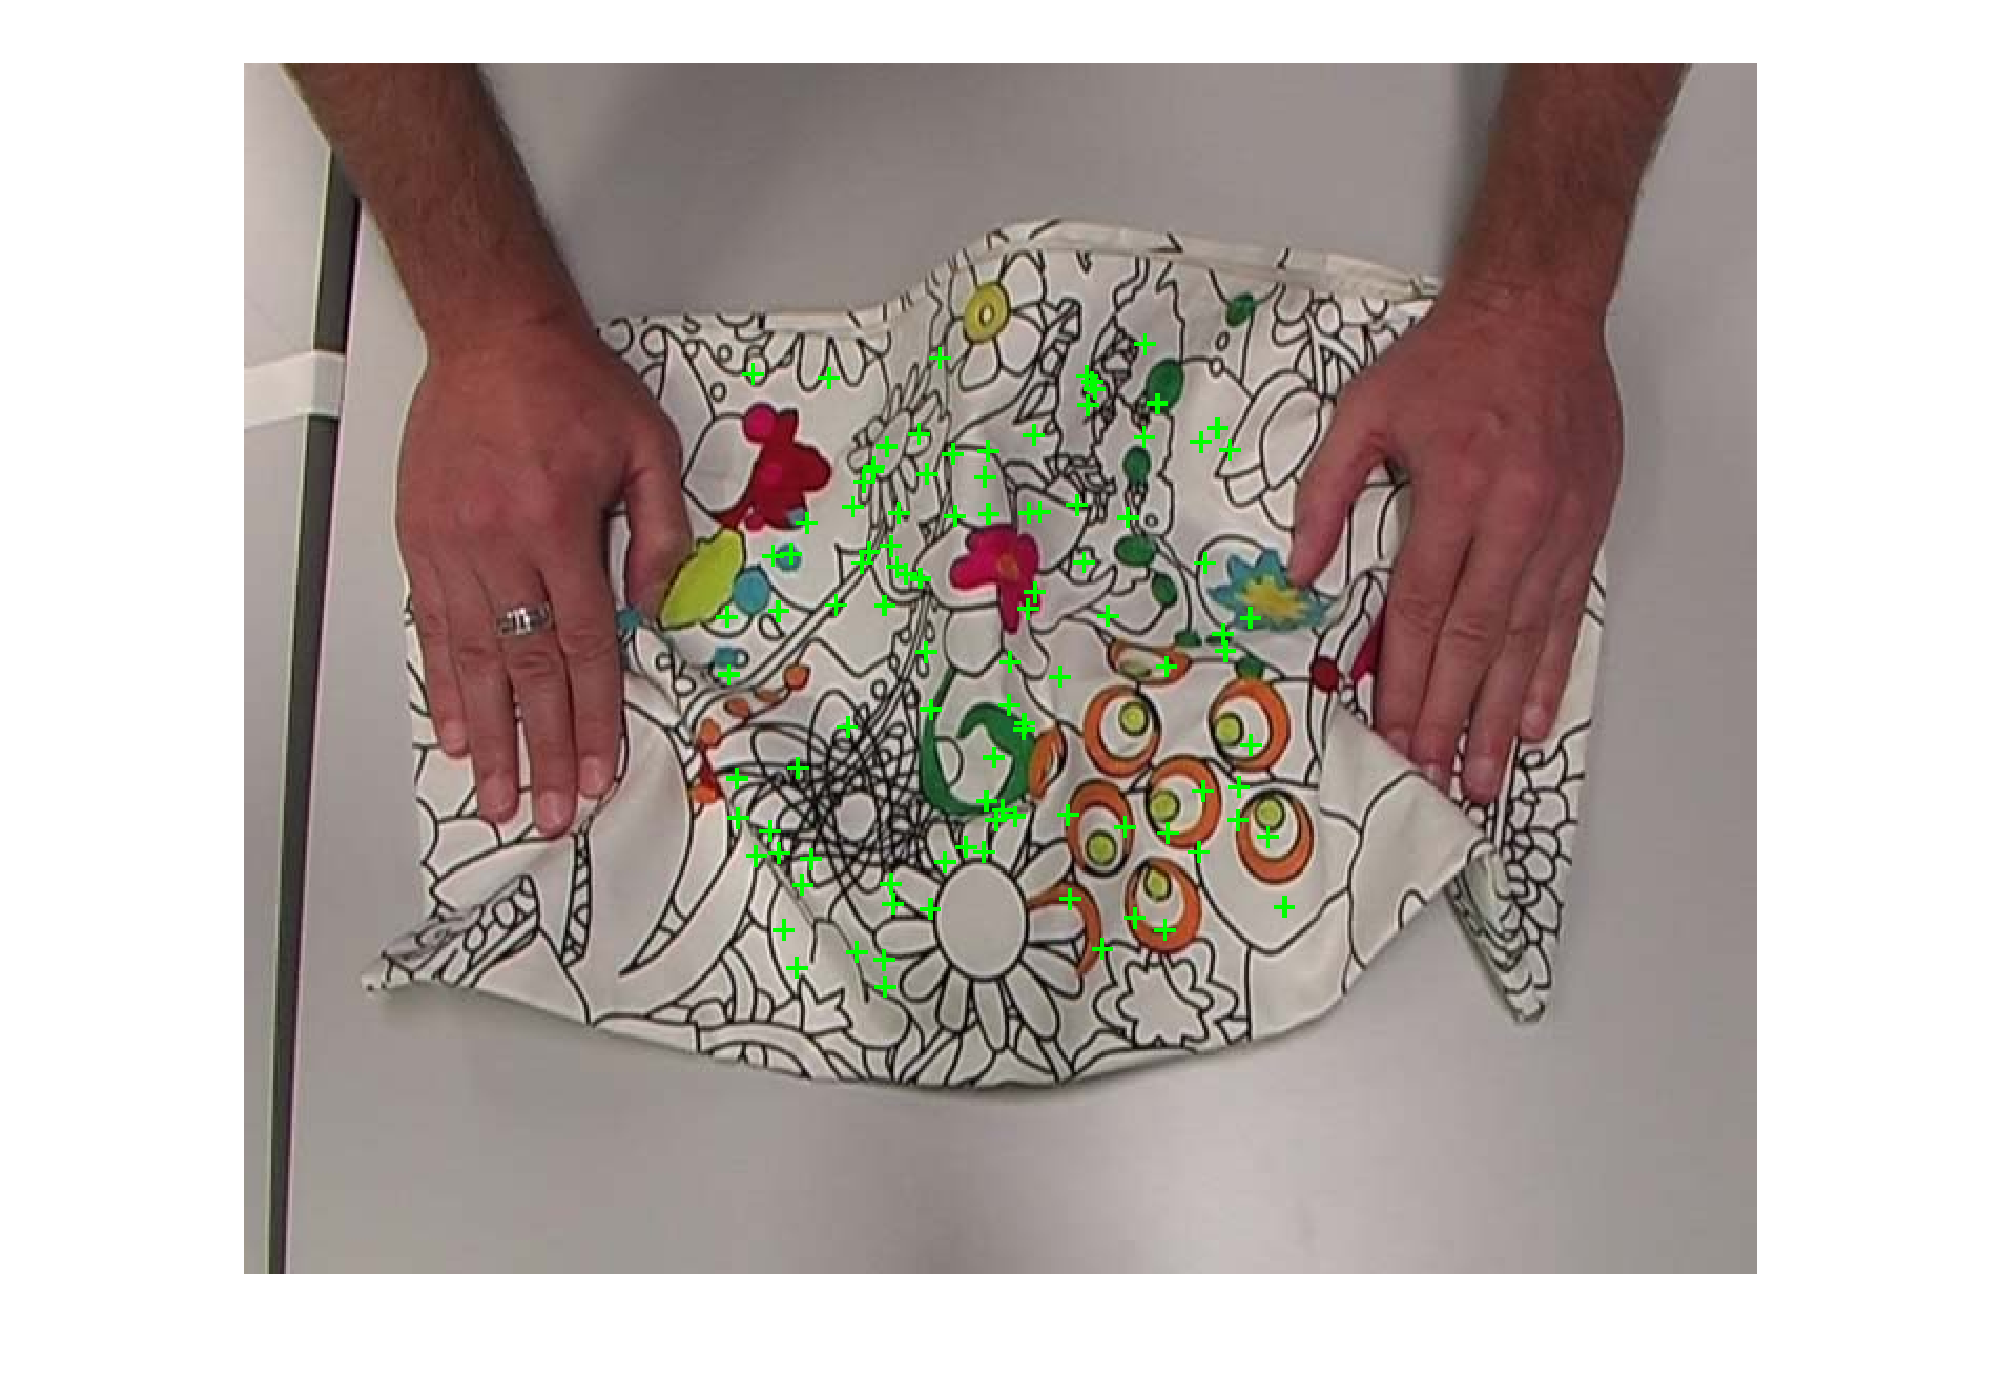
\includegraphics[width=36mm]{cushion_213.pdf}}%
        \end{minipage}%
        \hspace{5mm}%
        \addtocounter{subfigure}{-1}
        %%%
        \begin{minipage}[b]{0.2\textwidth}
            \subfigure[\scriptsize Frame 375]{
            \label{fig:subfig:paperc1}
            \centering
            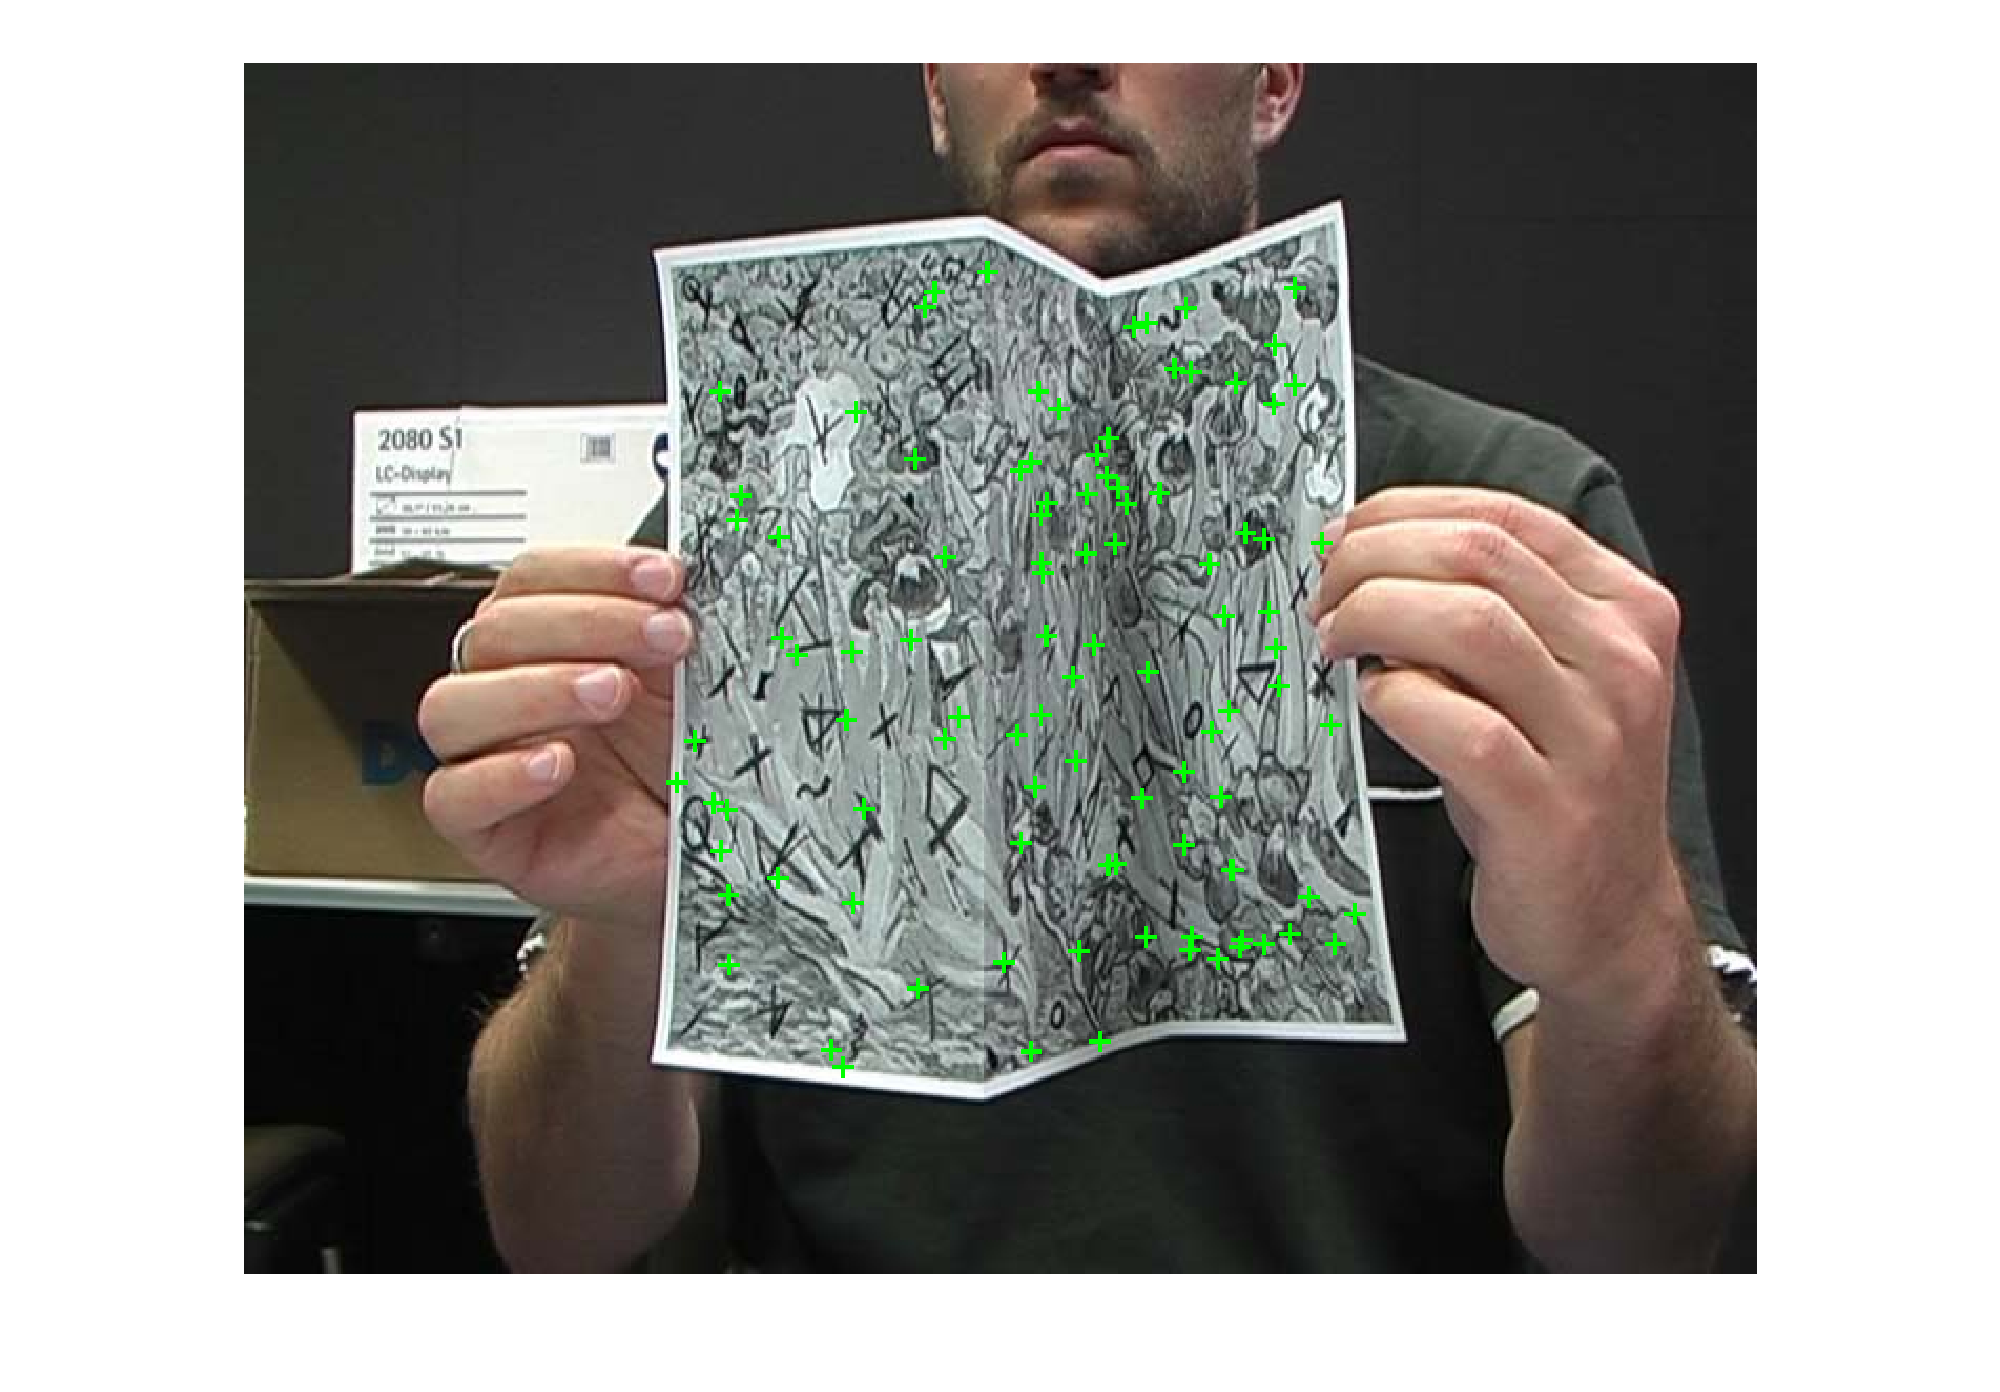
\includegraphics[width=36mm]{paperC_375.pdf}}%
        \end{minipage}\\%
        %\hspace{22mm}%
        \addtocounter{subfigure}{-1}
        \caption{Left to right: point sets on the surface of a piece of cloth, a piece of smoothly curving paper, a creased cushion and a piece of creased paper. The frame number is below each image. }
\label{fig:mini:subfig_deformableimages} %% label for entire figure
\end{figure*}%
%----------------------------------------
%  deformable matching results IMAGES
%----------------------------------------
\begin{figure*}[!ht]
\setlength{\abovecaptionskip}{0mm}
\setlength{\belowcaptionskip}{-4mm}
\centering
\setlength\subfigcapskip{-2mm}
%\vspace{-2ex}
        \hspace{-8ex}
         %----------------------------
         %%% smac method
         %----------------------------
        \begin{minipage}[b]{0.4\textwidth}
        \subfigure{
            \label{fig:subfig:clothmatching1}
            \centering
            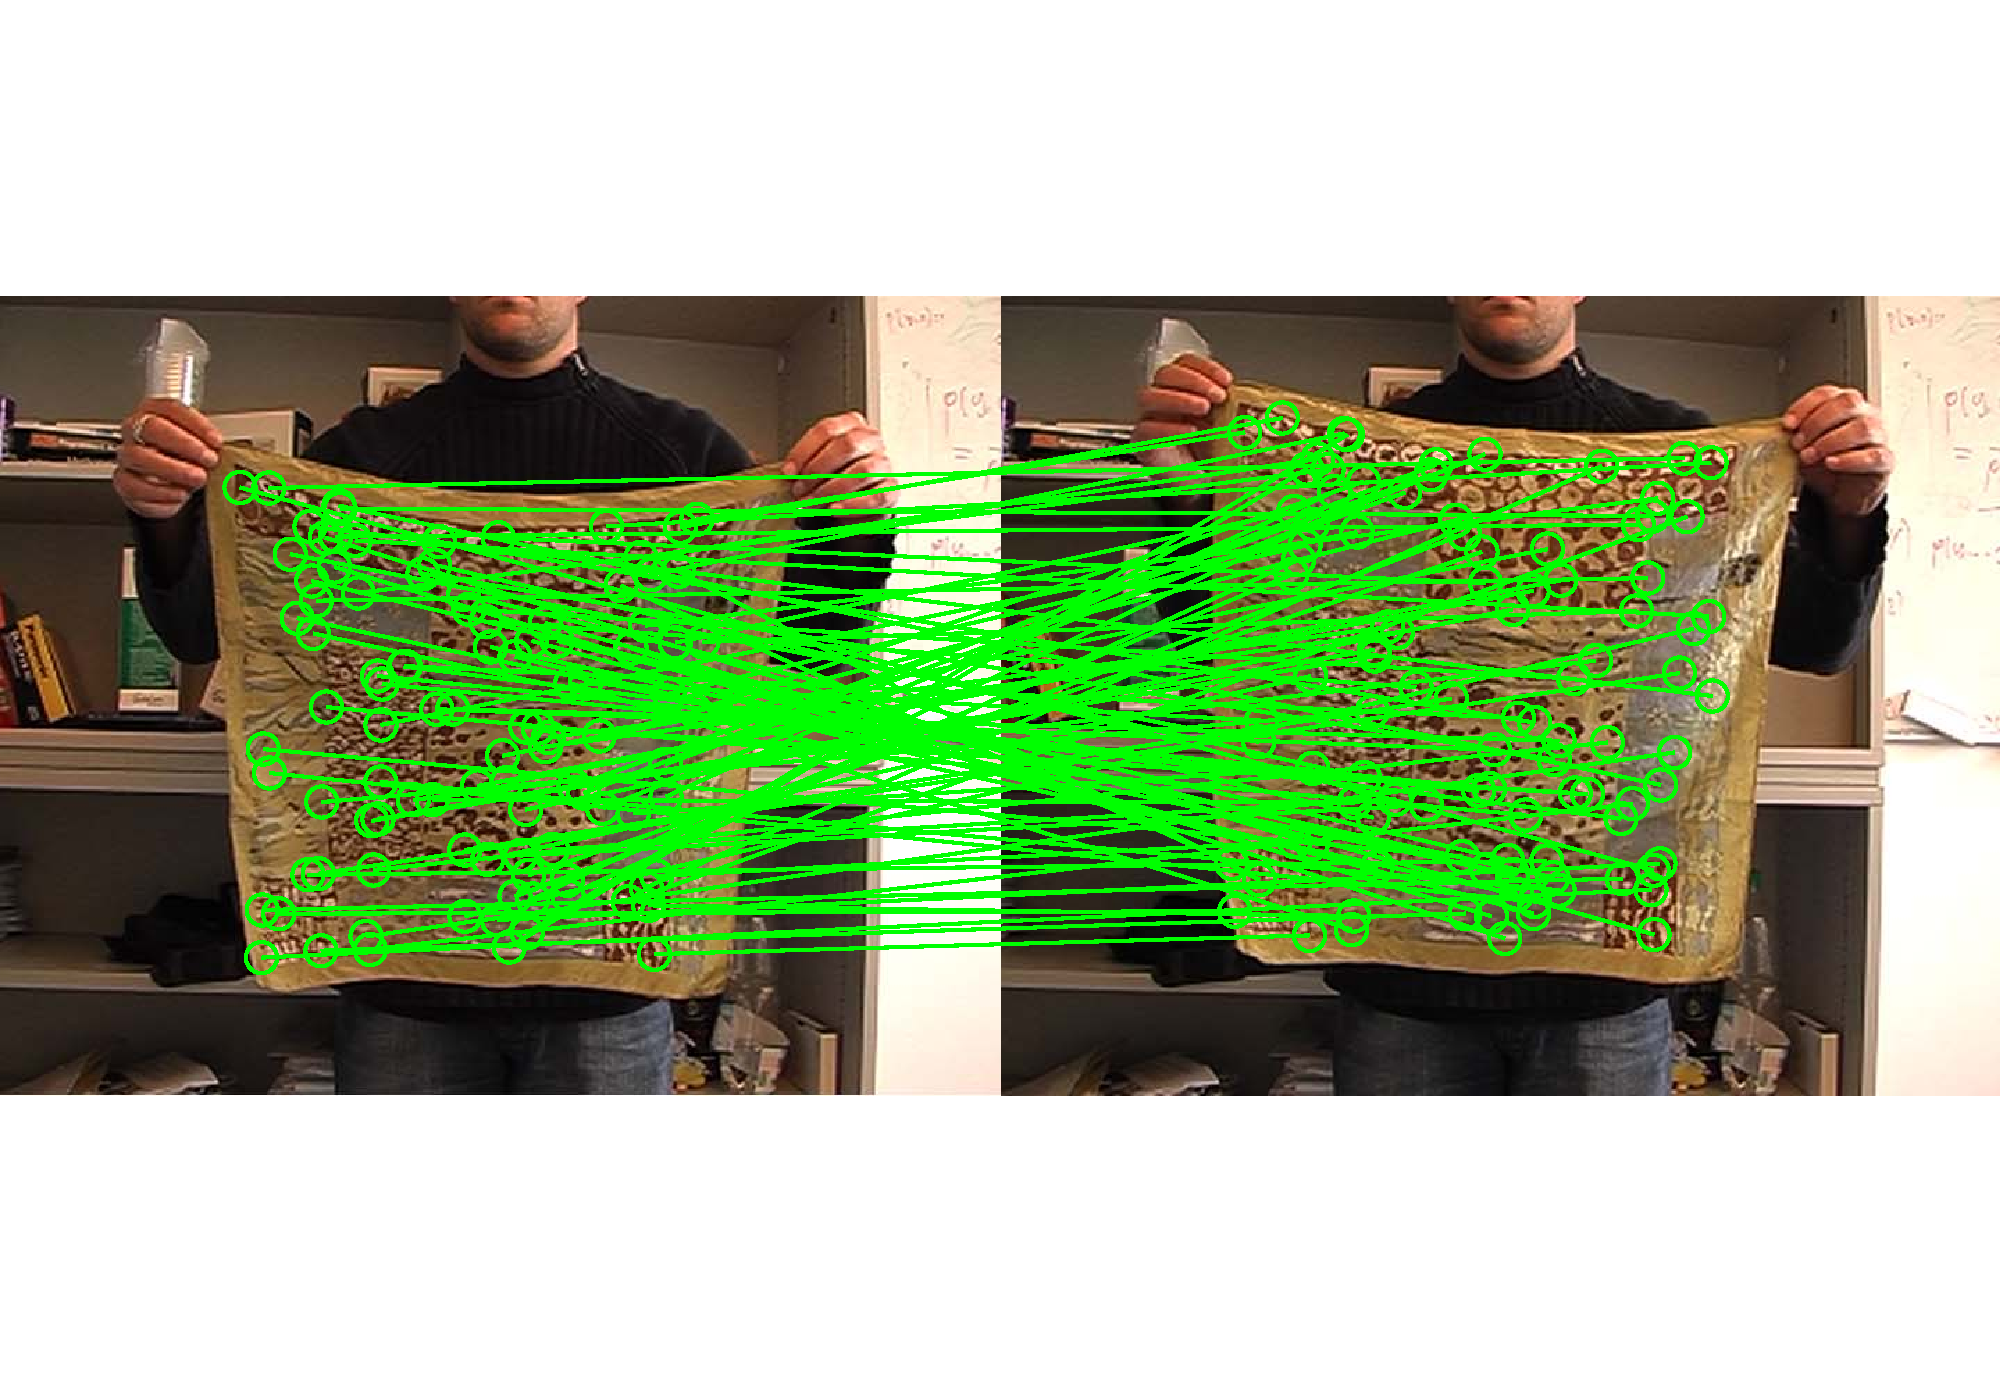
\includegraphics[width=62mm]{SMAC_F258-F299.pdf}%
            }%
        \end{minipage}%
        \hspace{8mm}%
        \addtocounter{subfigure}{-1}
        %%%
        \begin{minipage}[b]{0.4\textwidth}
        \subfigure{
            \label{fig:subfig:clothmatching2}
            \centering
            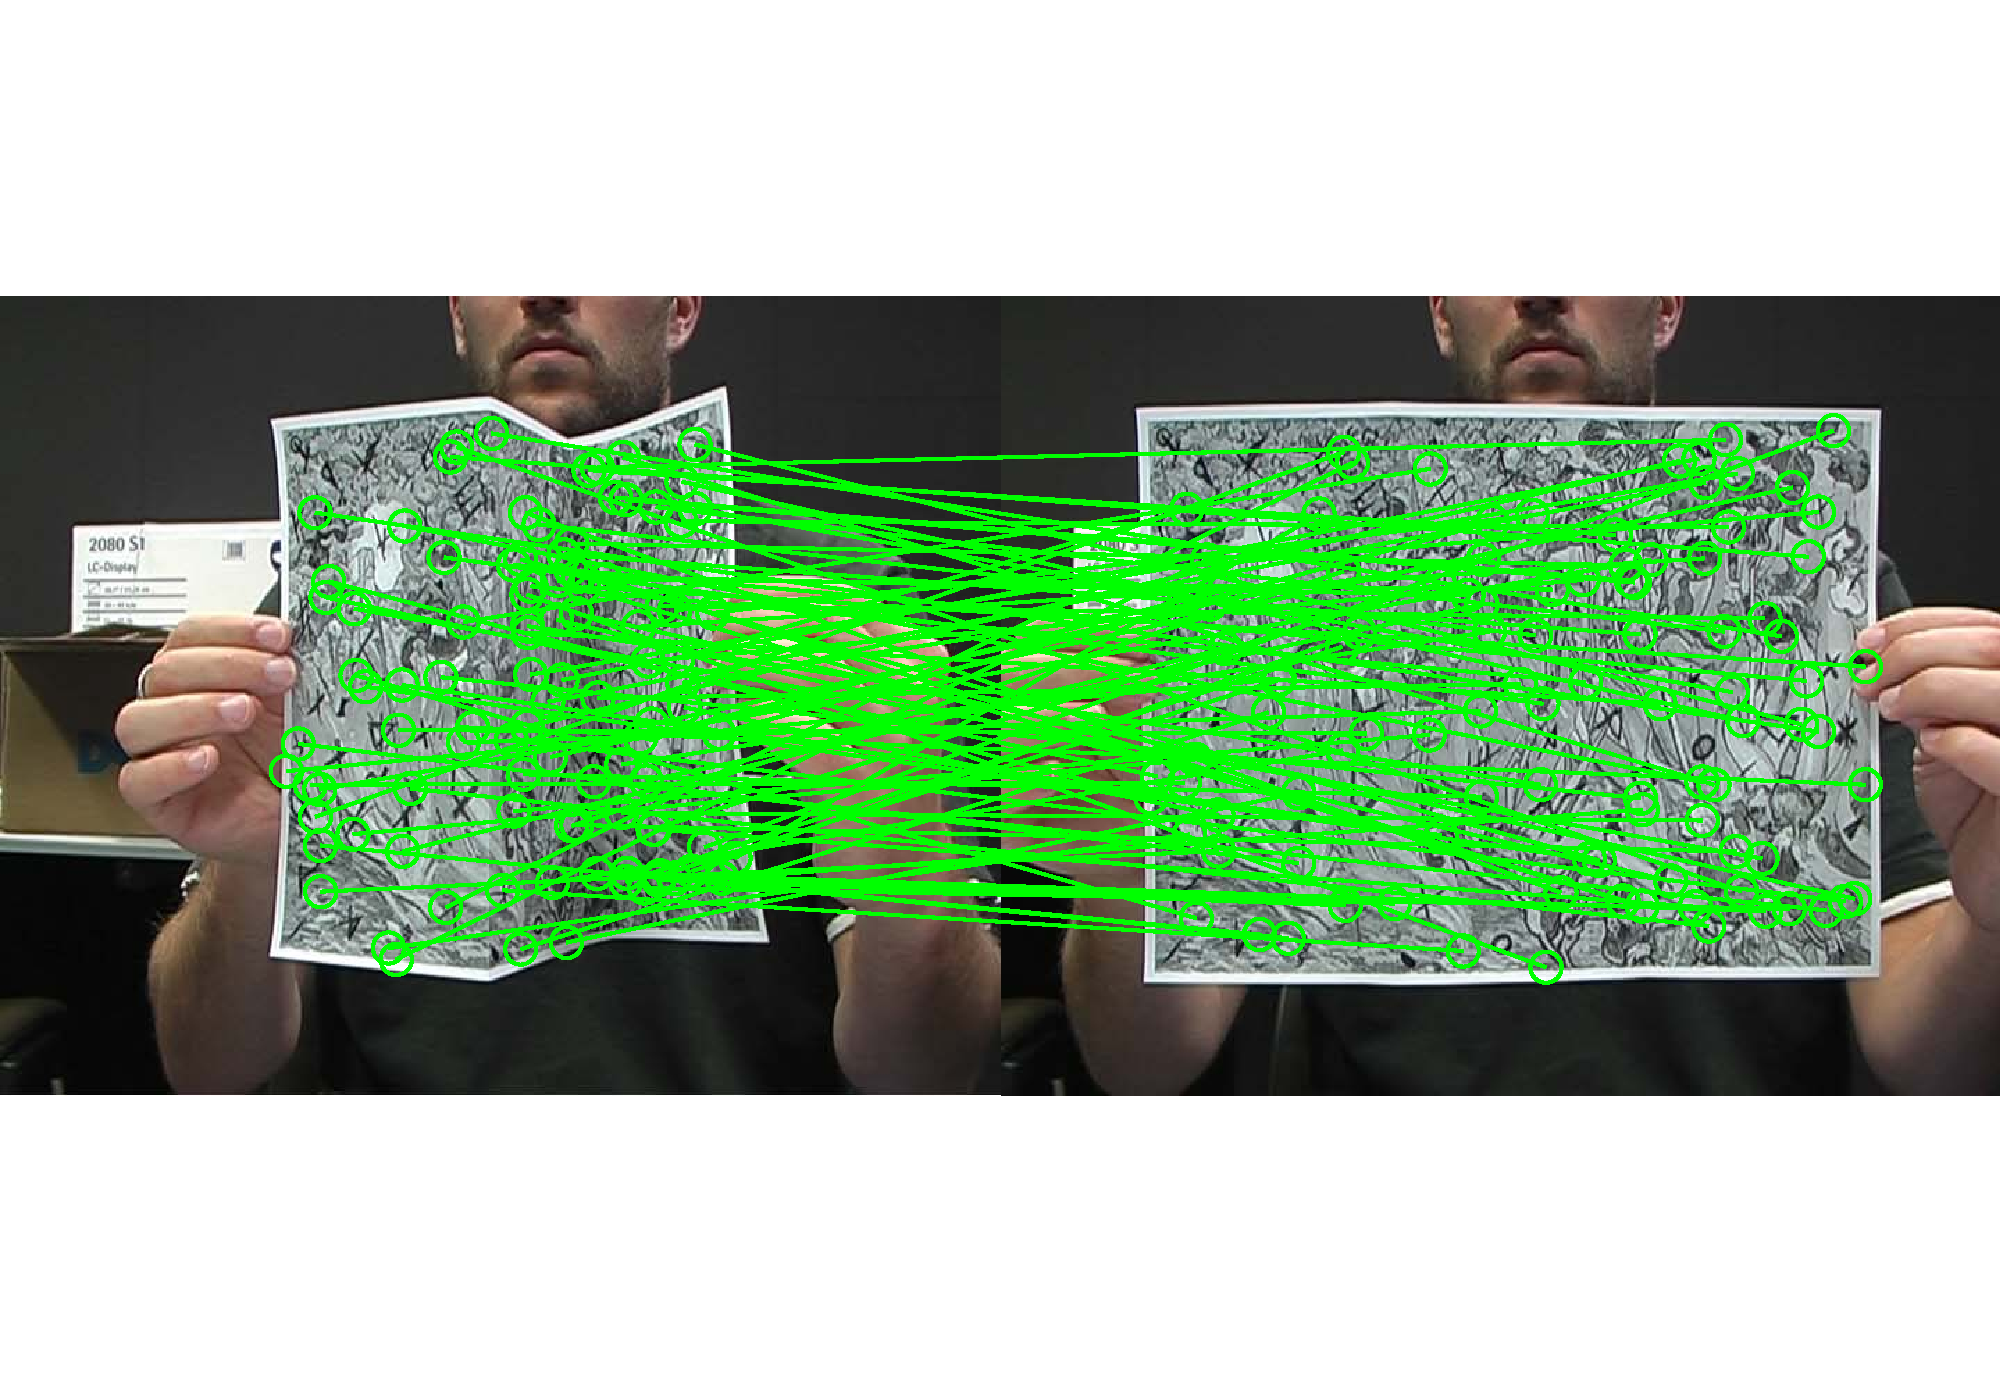
\includegraphics[width=60mm]{SMAC_F309-375.pdf}%
            }%
        \end{minipage}\\%
        %\hspace{28mm}%
        \addtocounter{subfigure}{-1}%
        %----------------------------
        %%% HYPER method
        %----------------------------
        \hspace{-8ex}
        \begin{minipage}[b]{0.4\textwidth}
        \subfigure{
            \label{fig:subfig:clothmatching3}
            \centering
            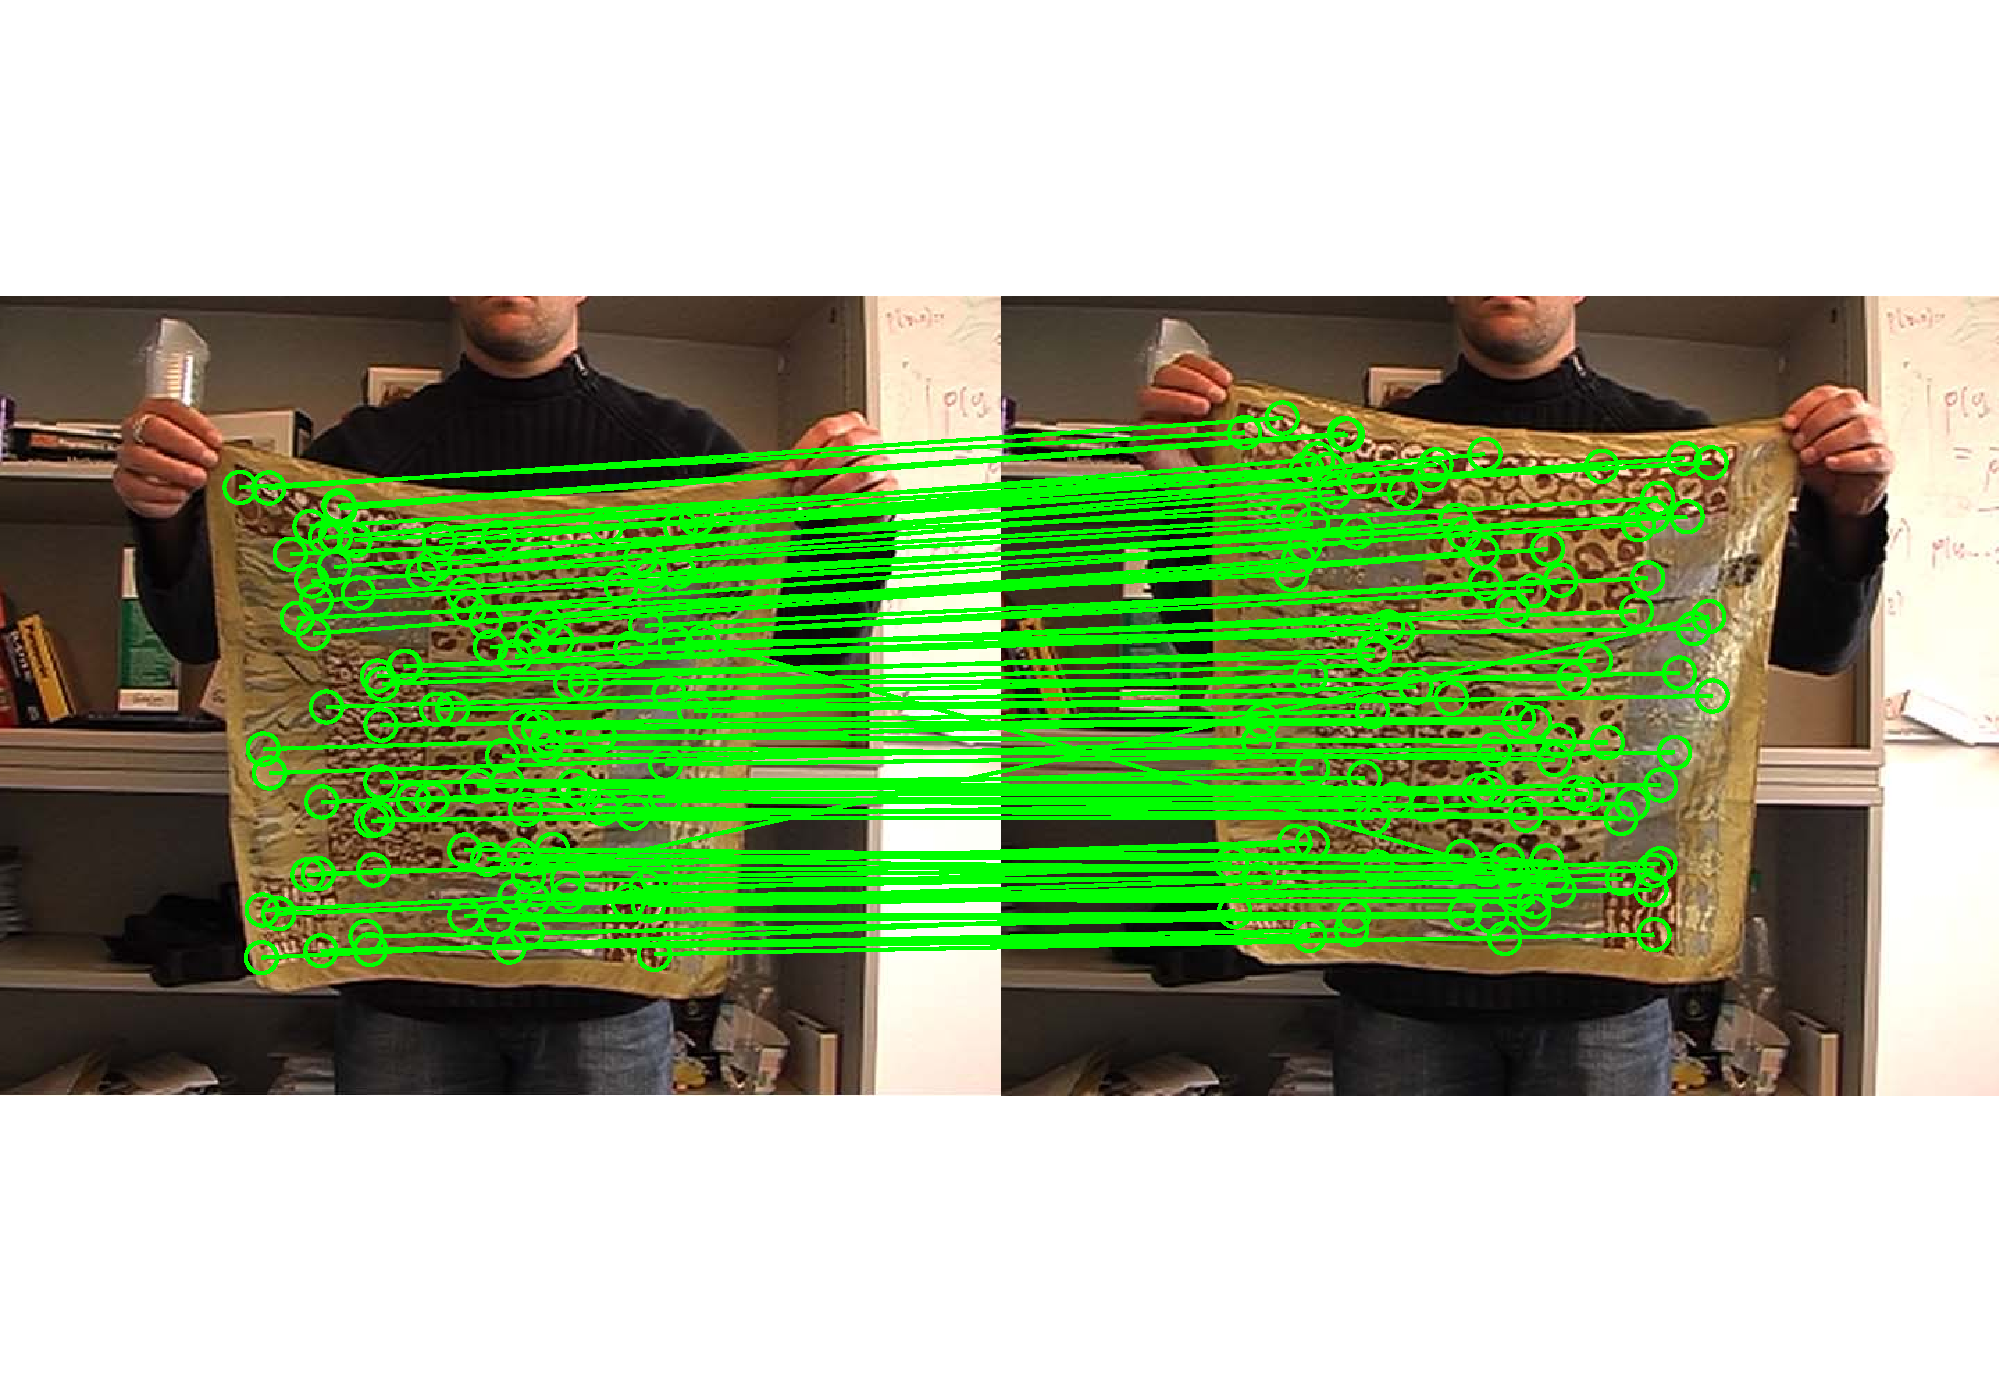
\includegraphics[width=62mm]{hyper_F258-F299.pdf}%
            }%
        \end{minipage}%
        \hspace{10mm}%
        \addtocounter{subfigure}{-1}%
        %%%
        \begin{minipage}[b]{0.4\textwidth}
        \subfigure{
            \label{fig:subfig:clothmatching4}
            \centering
            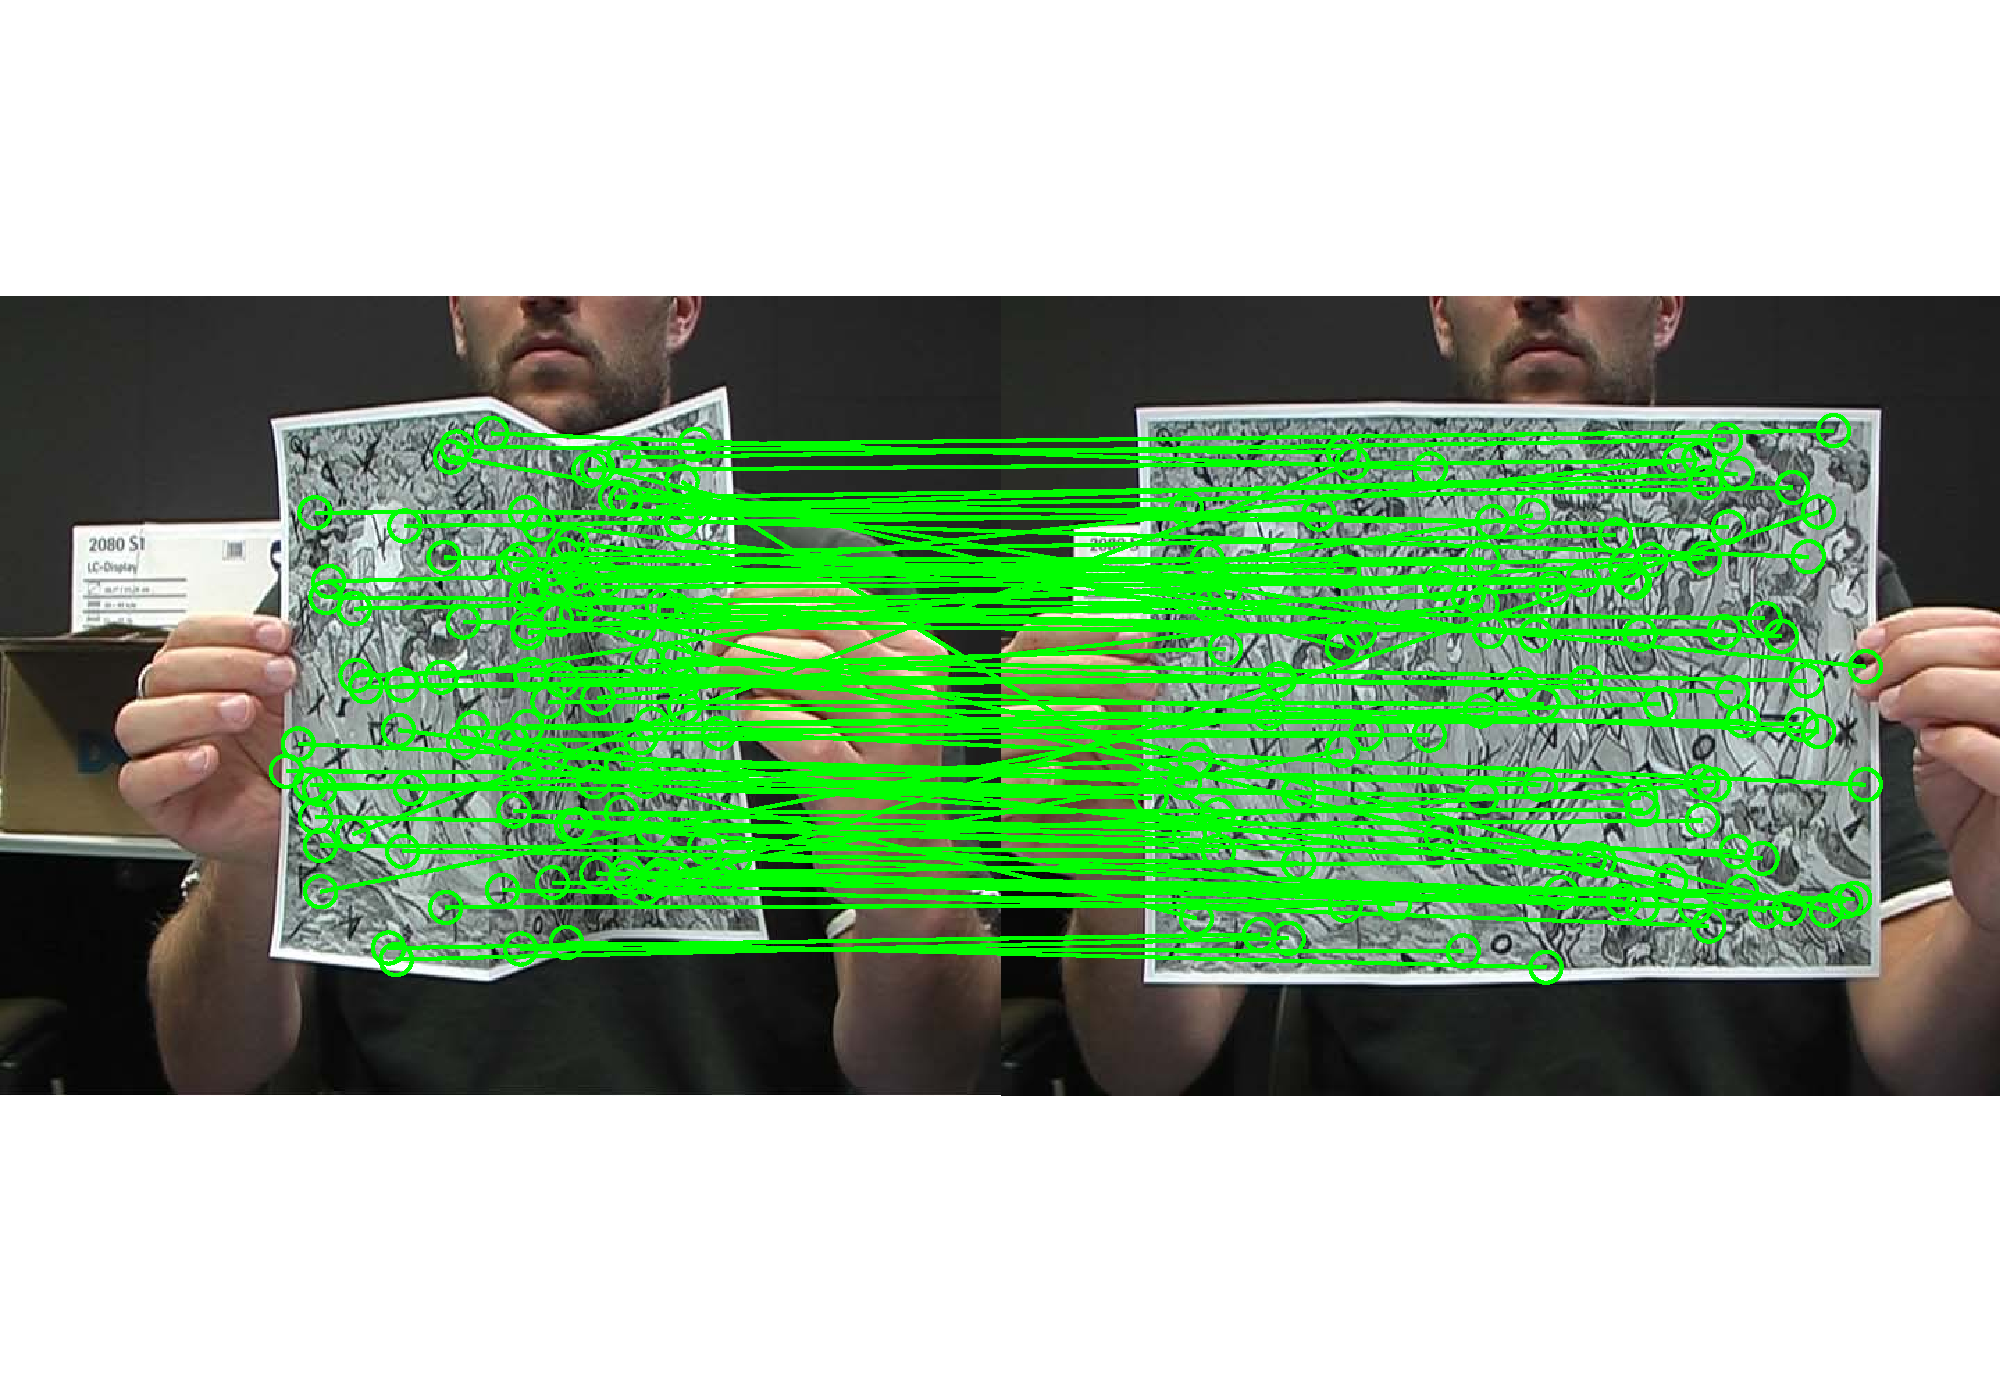
\includegraphics[width=60mm]{hyper_F309-375.pdf}%
            }%
        \end{minipage}\\%
        %\hspace{-16ex}%
        \addtocounter{subfigure}{-1}%
        %----------------------------
        %%% DEMO method
        %----------------------------
        \hspace{-8ex}
        \begin{minipage}[b]{0.4\textwidth}
        \subfigure{
            \label{fig:subfig:papercmatching1}
            \centering
            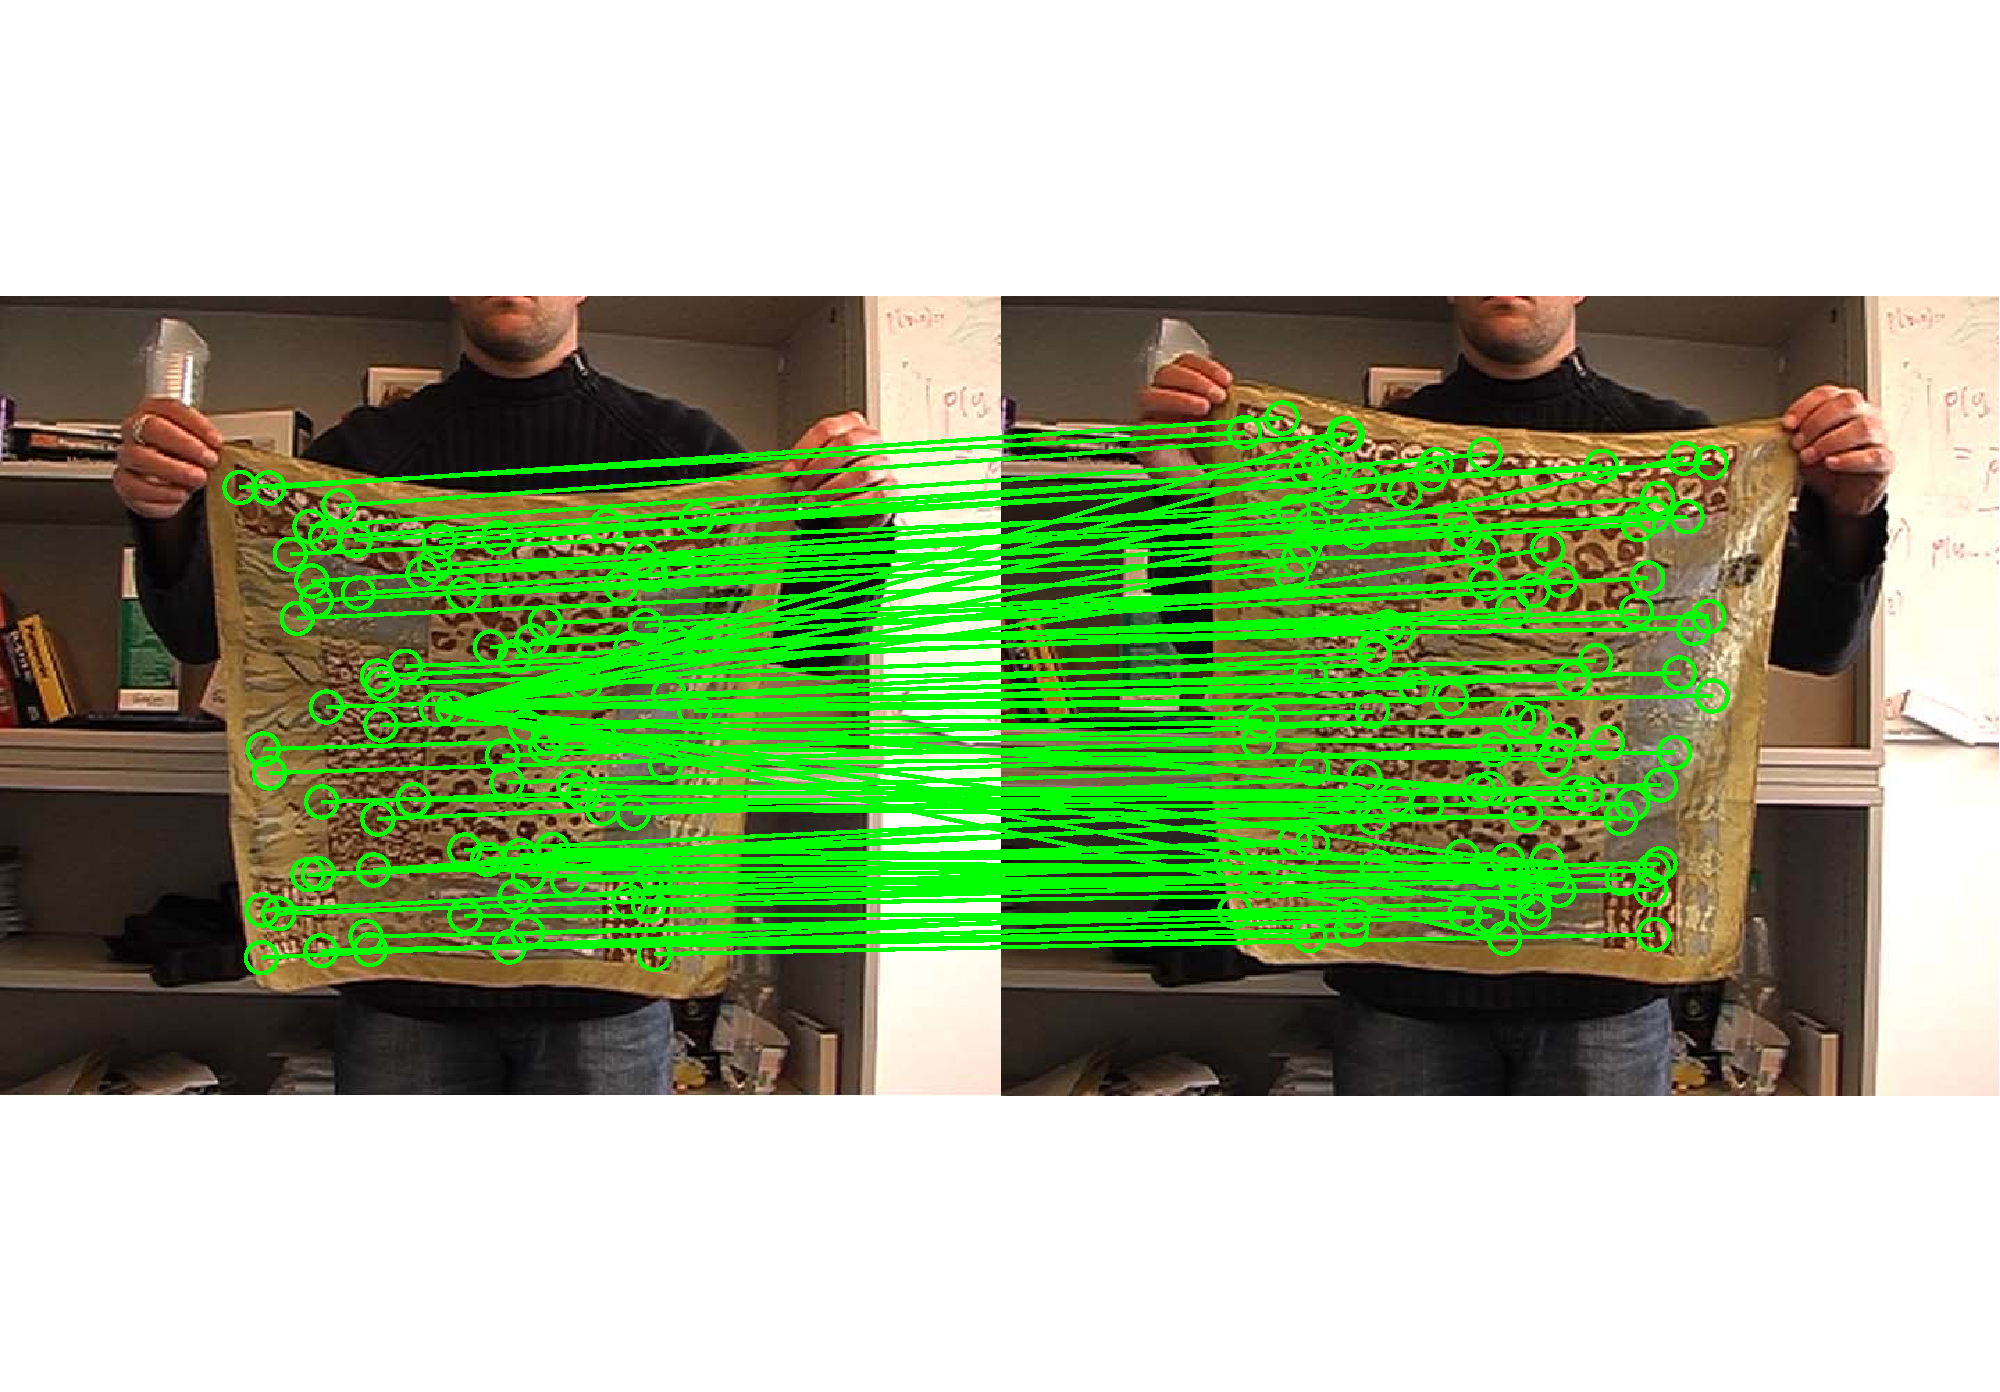
\includegraphics[width=62mm]{3demo_F258-F299.pdf}%
            }%
        \end{minipage}%
        \hspace{10mm}%
        \addtocounter{subfigure}{-1}%
        %%%
        \begin{minipage}[b]{0.4\textwidth}
        \subfigure{
            \label{fig:subfig:papercmatching2}
            \centering
            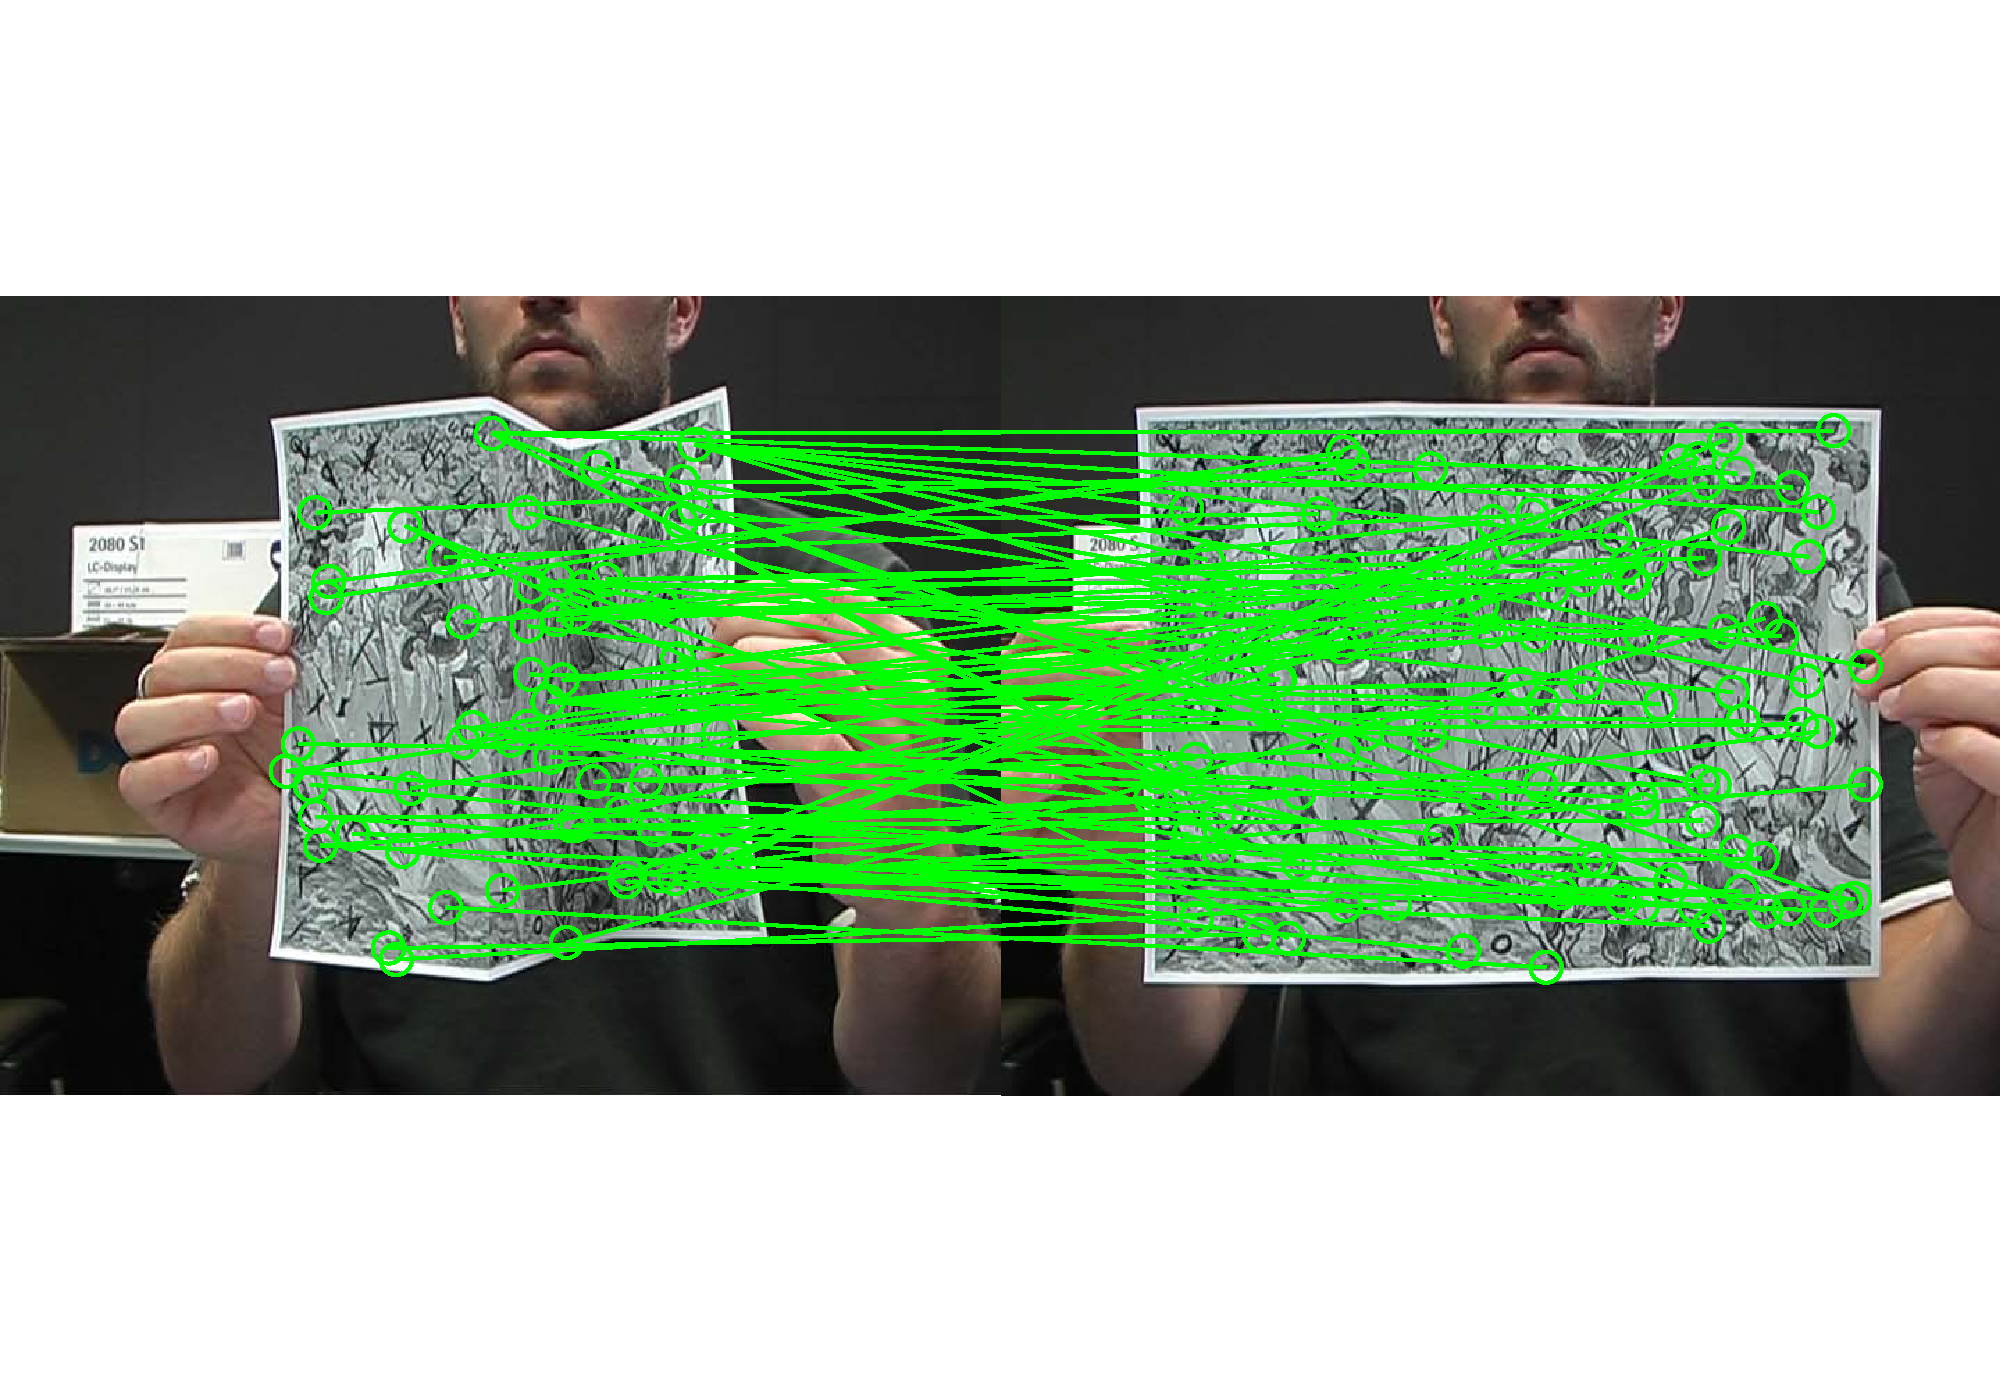
\includegraphics[width=60mm]{3demo_F309-375.pdf}%
            }%
        \end{minipage}\\%
        %\hspace{28mm}%
        \addtocounter{subfigure}{-1}%
        %----------------------------
        %%% OUR method
        %----------------------------
        \hspace{-8ex}
        \begin{minipage}[b]{0.4\textwidth}
        \subfigure[]{
            \label{fig:subfig:papercmatching3}
            \centering
            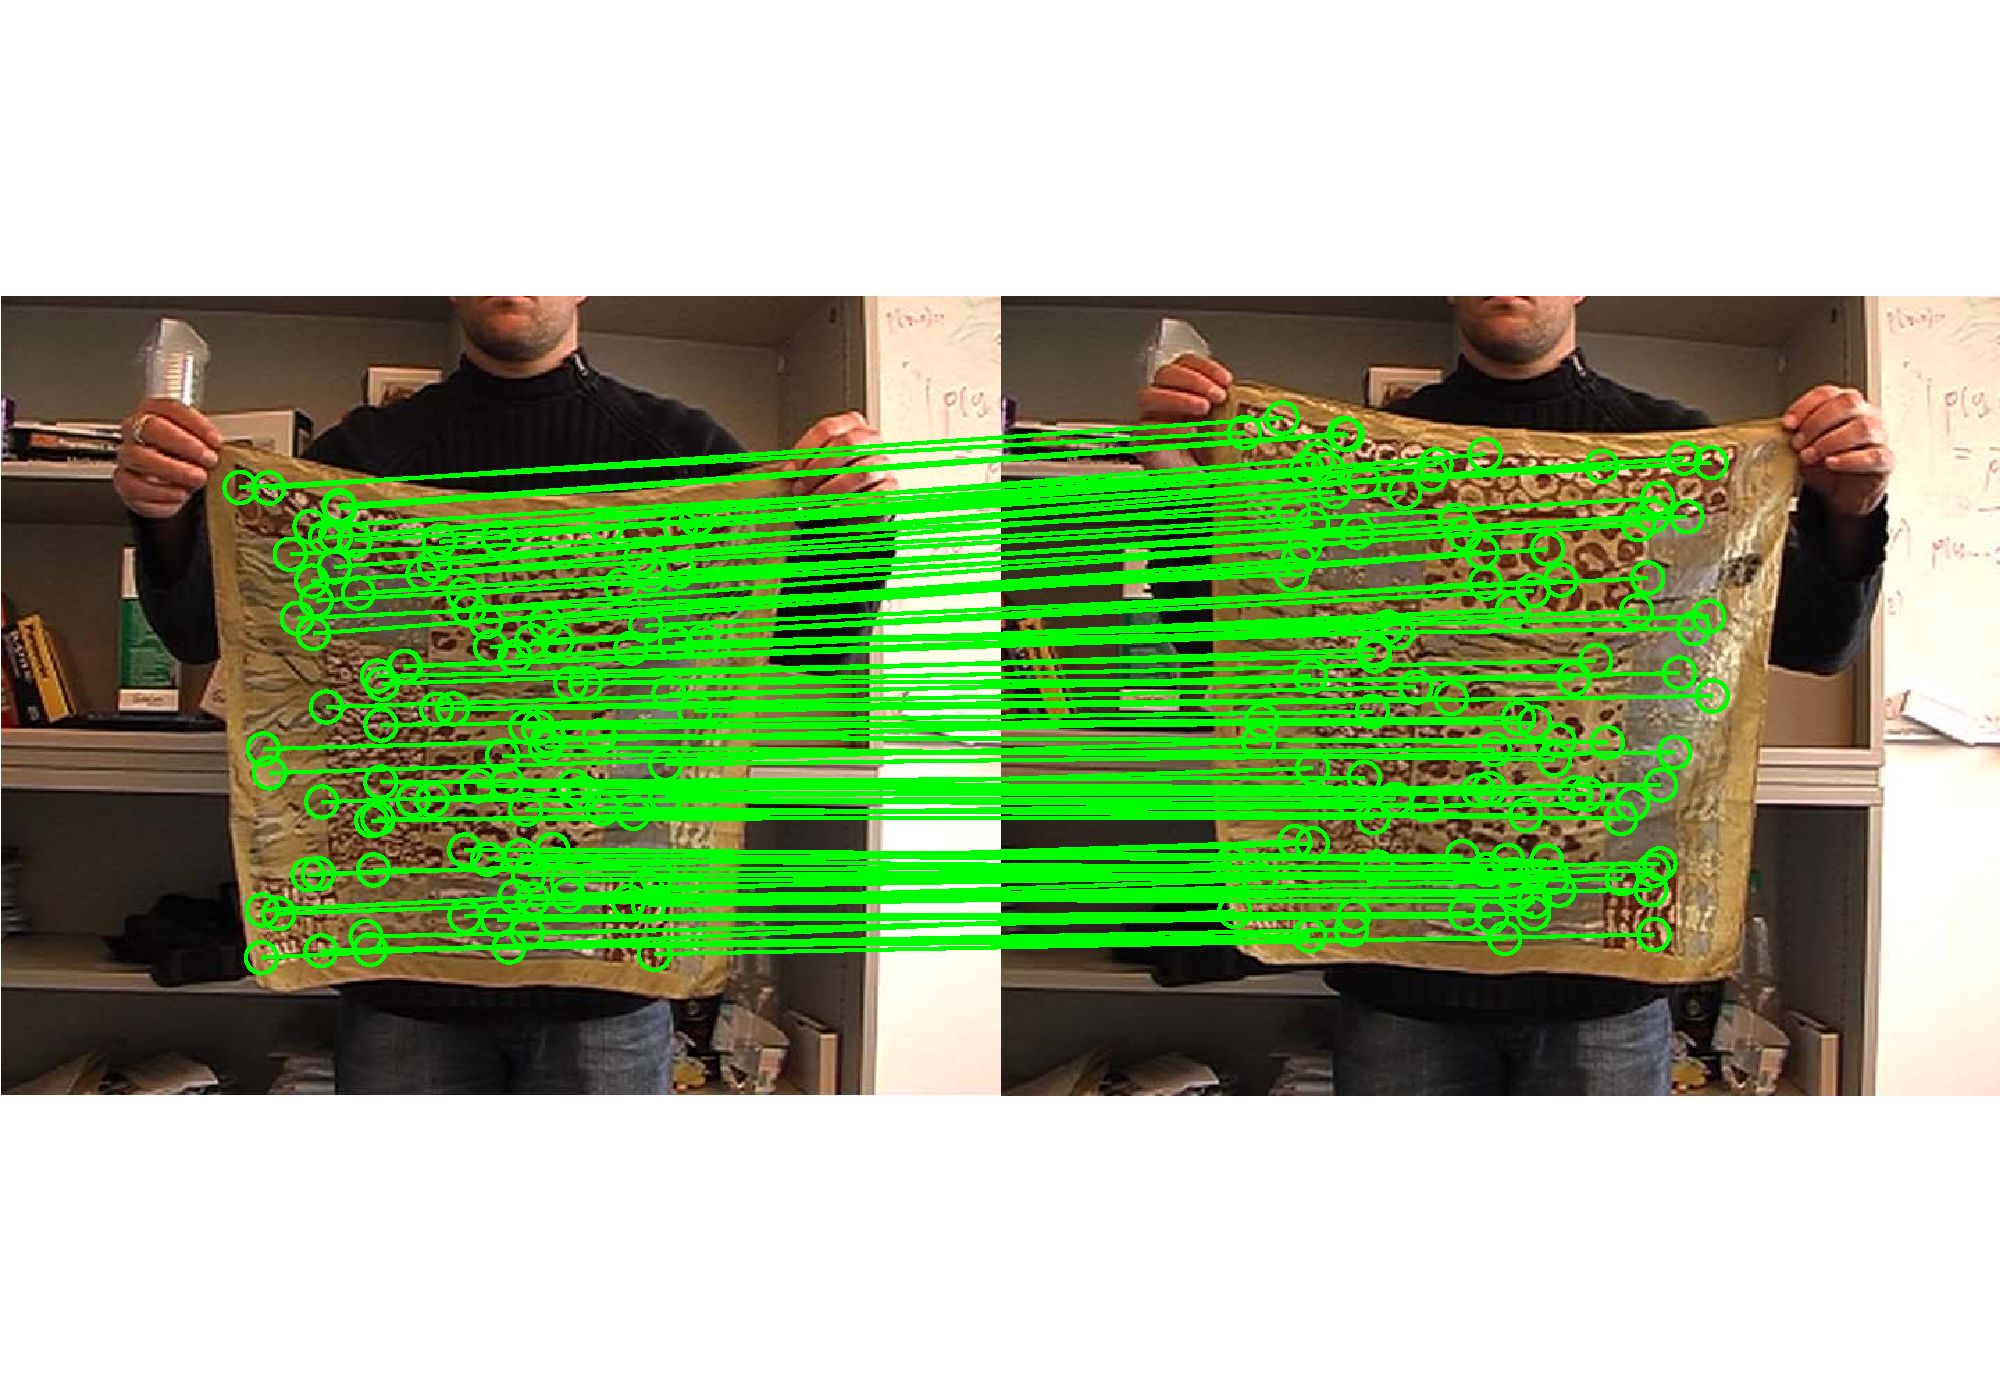
\includegraphics[width=60mm]{our_F258-F299.pdf}%
            }%
        \end{minipage}%
        \hspace{10mm}%
        %\addtocounter{subfigure}{-1}
        %%%
        \begin{minipage}[b]{0.4\textwidth}
        \subfigure[]{
            \label{fig:subfig:papercmatching4}
            \centering
            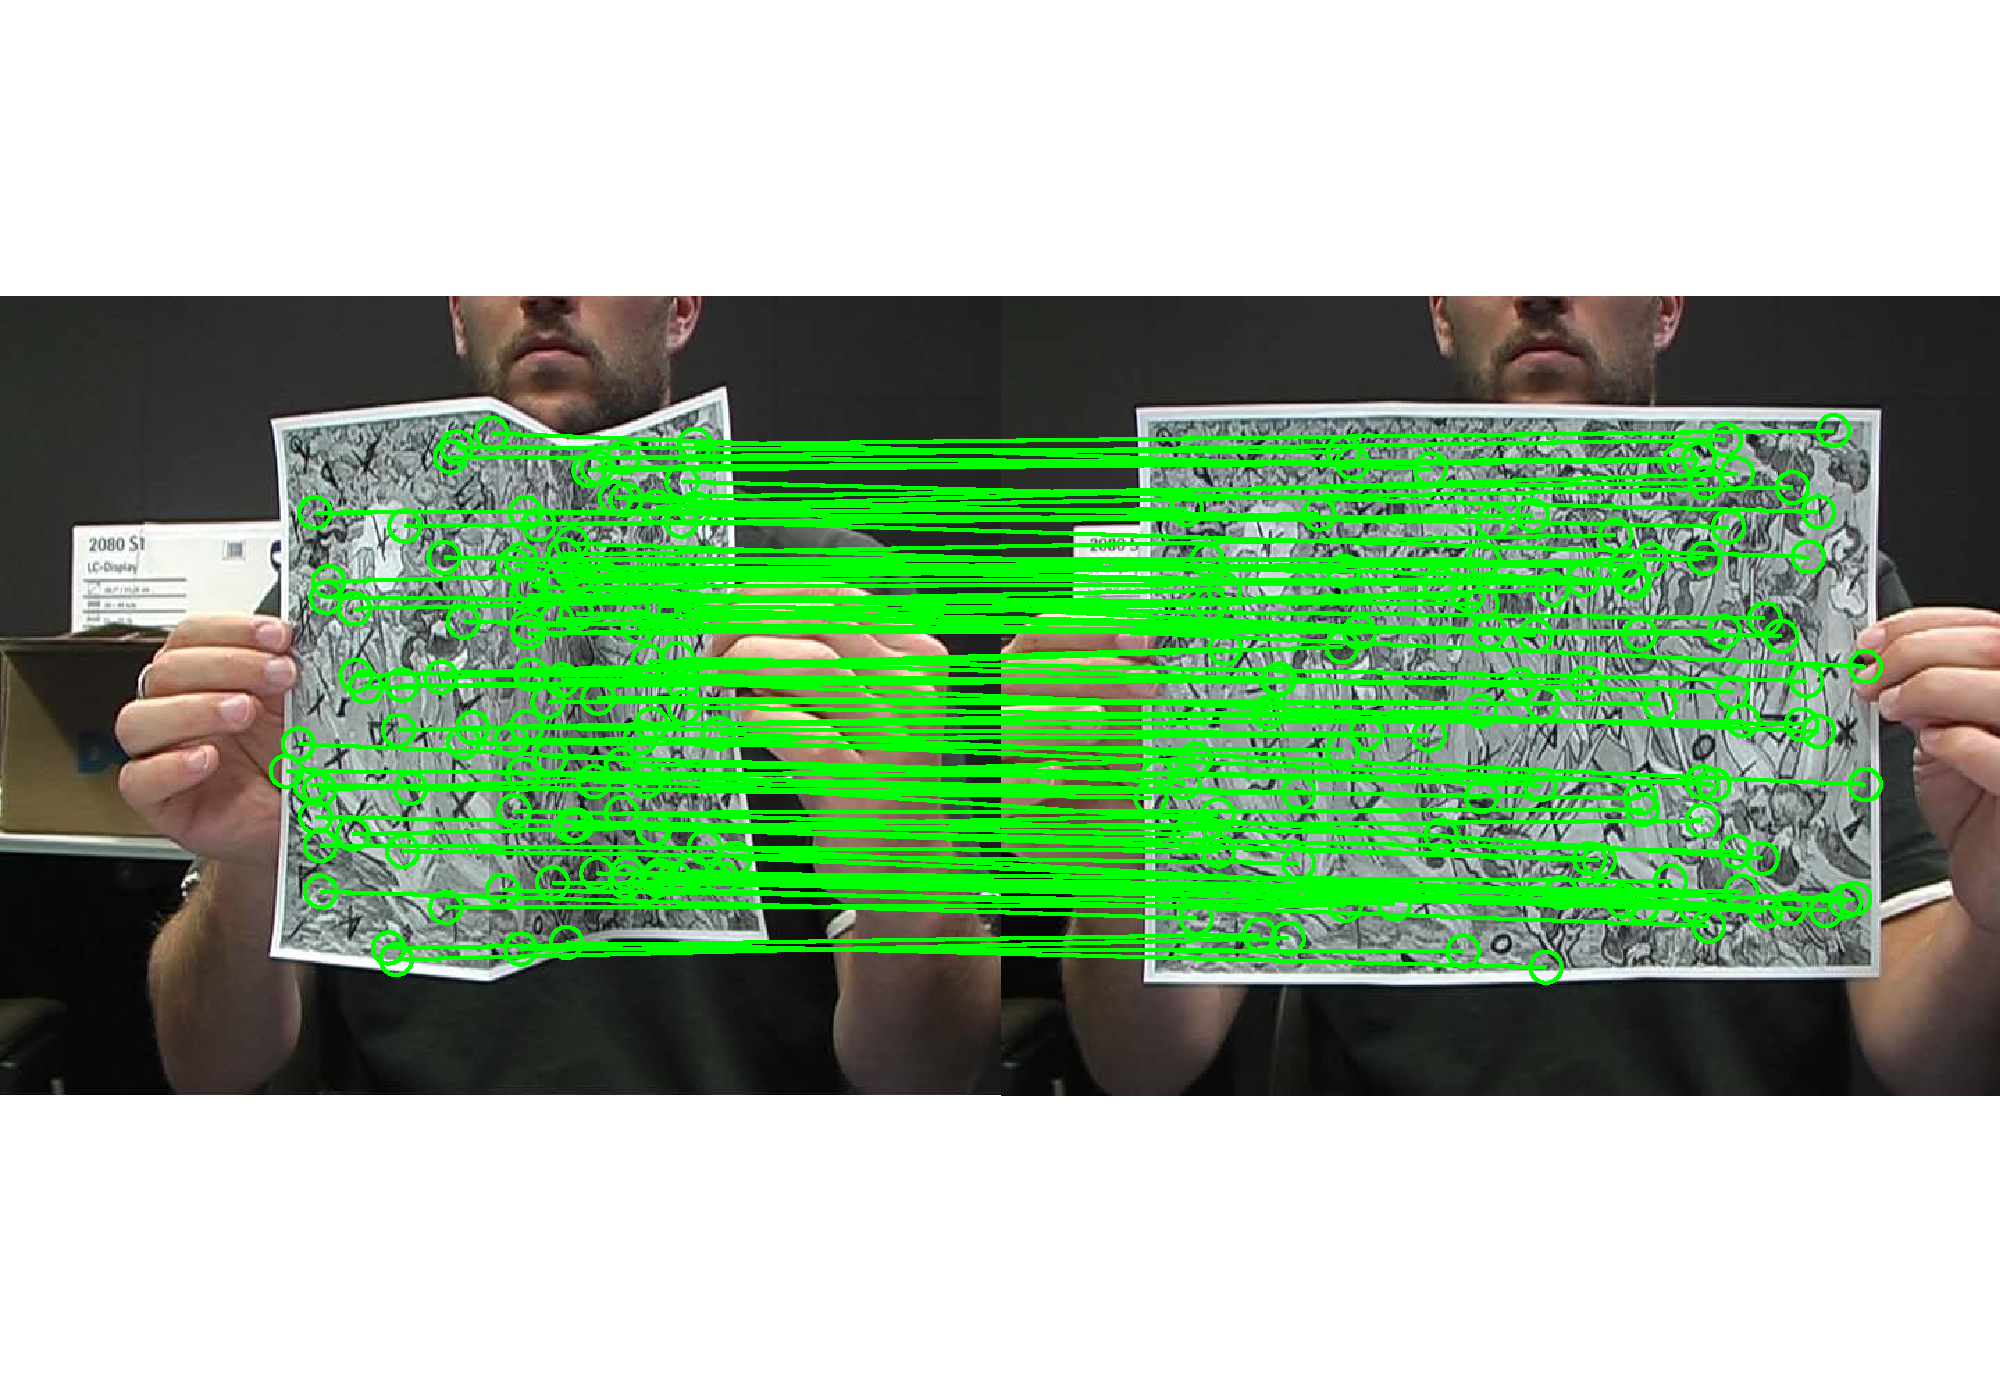
\includegraphics[width=60mm]{our_F309-375.pdf}%
            }%
        \end{minipage}%
        %\hspace{24mm}%
        %\addtocounter{subfigure}{-1}
        \caption{Matching results. Left: cloth set, frames 258 and299, right: creased paper set, frames 309  and 375. Top to bottom, spectral method~\cite{Cour06}, hyper graph matching method~\cite{Zass08}, a tensor based method~\cite{Duchenne_etal09} and our method.}
\label{fig:mini:deformablematchingimages} %% label for entire figure
%\vspace{-2ex}
\end{figure*}%
%----------------------------------------
%  deformable matching results TABLE
%----------------------------------------
\begin{table*}[!hp]
%\vspace{-4mm}
%\centering
\renewcommand{\arraystretch}{0.6}
\setlength{\aboverulesep}{0pt}
\setlength{\belowrulesep}{0pt}
\caption{Error rate of deformable surface matching.}
\hspace{-5ex}
\label{tab:errorrate1}
\begin{tabular}{c|c c c c c|c c c c c}
\toprule
\itshape \small{Dataset}  & \multicolumn{5}{|c|}{\itshape \small{cloth}}  & \multicolumn{5}{c}{\itshape \small{bending paper}} \\
\hline
\itshape \small{Matching} & \itshape \footnotesize{F88-}	& \itshape \footnotesize{F107-}	& \itshape\footnotesize{F120-}	& \itshape\footnotesize{F258-} & \itshape\footnotesize{F305-} & \itshape\footnotesize{F262-}	& \itshape\footnotesize{F275-}	& \itshape\footnotesize{F280-} & \itshape\footnotesize{F289-}	& \itshape\footnotesize{F301-}  \\
\itshape \small{frames}   & \itshape \footnotesize{F299}     & \itshape \footnotesize{F299}   & \itshape \footnotesize{F299}   &                \itshape \footnotesize{F299}  & \itshape \footnotesize{F299}  & \itshape\footnotesize{F314}    & \itshape \footnotesize{F314}   &                \itshape \footnotesize{F314}  & \itshape \footnotesize{F314}   & \itshape \footnotesize{F314} \\
\hline
\itshape \small{Our method} & \footnotesize 0	& \footnotesize 0	    & \footnotesize 0	    & \footnotesize 0	    & \footnotesize 0	  & \footnotesize0	        & \footnotesize 0	    & \footnotesize 0	    & \footnotesize 0	    &  \footnotesize 0  \\
%\hline
\itshape \small{\cite{Zass08}} &	 \footnotesize{2\%}	& \footnotesize{2\%}	&  \footnotesize{2\%}	& \footnotesize{2\%}	& \footnotesize{2\%} & \footnotesize{23\%}	 &  \footnotesize{9\%}	 & \footnotesize{23\%}	& \footnotesize{18\%}	& \footnotesize{14\%}  \\
%\hline
\itshape \small{\cite{Duchenne_etal09}} & \footnotesize{25\%} & \footnotesize{41\%}   & \footnotesize{30\%}	& \footnotesize{30\%}	 & \footnotesize{42\%}	& \footnotesize{71\%}	 & \footnotesize{67\%}	& \footnotesize{59\%}	& \footnotesize{55\%}	& \footnotesize{50\%}  \\
%\hline
\itshape \small{\cite{Cour06}}      & \footnotesize{93\%} & \footnotesize{83\%}	&  \footnotesize{77\%}	&  \footnotesize{94\%}	& \footnotesize{90\%}	 & \footnotesize{93\%}	 & \footnotesize{98\%}	 & \footnotesize{99\%}	& \footnotesize{93\%}	& \footnotesize{96\%}  \\
\bottomrule
\end{tabular}%
%\vspace{-27pt}
%\vspace{-8mm}
\end{table*}%
%
\begin{table*}[!htbp]
%\vspace{-15pt}
%\centering
\renewcommand{\arraystretch}{0.6}
\setlength{\aboverulesep}{0pt}
\setlength{\belowrulesep}{0pt}
\caption{Error rate of deformable surface matching.}
\label{tab:errorrate2}
\hspace{-5ex}
\begin{tabular}{c|c c c c c|c c c c c}
\toprule
\itshape \small{Dataset}  & \multicolumn{5}{|c|}{\itshape \small{cushion}}  & \multicolumn{5}{c}{\itshape \small{creased paper}} \\
\hline
\itshape \small{Matching} & \itshape \footnotesize{F144-}	& \itshape \footnotesize{F156-}	& \itshape\footnotesize{F165-}	& \itshape\footnotesize{F172-} & \itshape\footnotesize{F188-} & \itshape\footnotesize{F309-}	& \itshape\footnotesize{F320-}	& \itshape\footnotesize{F330-} & \itshape\footnotesize{F340-}	& \itshape\footnotesize{F352-}  \\
\itshape \small{frames}   & \itshape \footnotesize{F213}     & \itshape \footnotesize{F213}   & \itshape \footnotesize{F213}   &                \itshape \footnotesize{F213}  & \itshape \footnotesize{F213}  & \itshape\footnotesize{F375}    & \itshape \footnotesize{F375}   &                \itshape \footnotesize{F375}  & \itshape \footnotesize{F375}   & \itshape \footnotesize{F375} \\
\hline
\itshape \small{Our method} & \footnotesize 0	& \footnotesize 0	    & \footnotesize 0	    & \footnotesize 0	    & \footnotesize 0	  & \footnotesize0	        & \footnotesize 0	    & \footnotesize 0	    & \footnotesize 0	    &  \footnotesize 0  \\
%\hline
\itshape \small{\cite{Zass08}} &	 \footnotesize{8\%}	& \footnotesize{10\%}	&  \footnotesize{2\%}	& \footnotesize{6\%}	& \footnotesize{5\%} & \footnotesize{22\%}	 &  \footnotesize{10\%}	 & \footnotesize{11\%}	& \footnotesize{2\%}	& \footnotesize{6\%}  \\
%\hline
\itshape \small{\cite{Duchenne_etal09}} & \footnotesize{61\%} & \footnotesize{65\%}   & \footnotesize{59\%}	& \footnotesize{49\%}	 & \footnotesize{30\%}	& \footnotesize{80\%}	 & \footnotesize{74\%}	& \footnotesize{77\%}	& \footnotesize{68\%}	& \footnotesize{46\%}  \\
%\hline
\itshape \small{\cite{Cour06}}      & \footnotesize{95\%} & \footnotesize{92\%}	&  \footnotesize{93\%}	&  \footnotesize{93\%}	& \footnotesize{92\%}	 & \footnotesize{98\%}	 & \footnotesize{94\%}	 & \footnotesize{96\%}	& \footnotesize{92\%}	& \footnotesize{88\%}  \\
\bottomrule
\end{tabular}%
%\vspace{10pt}
\end{table*}%

The matching accuracy is given as the number of correctly matched points (according to the provided ground truth) divided by the total number of points that could potentially be matched. The results for all methods, using the four image sets, are given in Tables~\ref{tab:errorrate1} and~\ref{tab:errorrate2} and are illustrated in Fig.\ref{fig:mini:deformablematchingimages}. Our method matched all the features on the deforming surfaces, while others did not.
In this test our method used 20000 feature tuples, while the method of~\cite{Duchenne_etal09} used 1010000 features  and the method of~\cite{Zass08} used$40000$. The average running time to match two feature sets each with $100$ features was around 8s for our method, 13s for \cite{Duchenne_etal09}, 6.5s for~\cite{Zass08}, and $5$s for~\cite{Cour06}. As above it can be seen that our method is both efficient and much more accurate than the other high-order methods~\cite{Zass08,Duchenne_etal09}.

%-------------------------------------------------------------------------
\subsection{Image matching under projective transformation}
\label{subsec:projectivedata}

Finally, we used a \texttt{house} data set\footnote{\url{From http://www.robots.ox.ac.uk/~vgg/data/data-mview.html}} to assess matching performance under perspective transformation. The data include ten different viewpoints under projective transformation, numbered from 0--9. The Harris corners in every frame are provided. We used the Harris corners in image 0 as feature set $P_1$, and those in other images as $P_2$. As ground truth correspondences are provided, we can directly compute the matching accuracy of the algorithm, as the number of correctly matched points divided by the total number of points that could potentially be matched.
All the higher-order methods used the same third-order potentials from Section~\ref{sec:implementation}, and equivalent tensor sizes.

%------------------------------
%  PROJECTION matching results
%------------------------------
\begin{figure*}[!t]
%\vspace{2mm}
%%\hspace{-8ex}
\setlength{\abovecaptionskip}{0mm}
\setlength{\belowcaptionskip}{-2mm}
\centering
     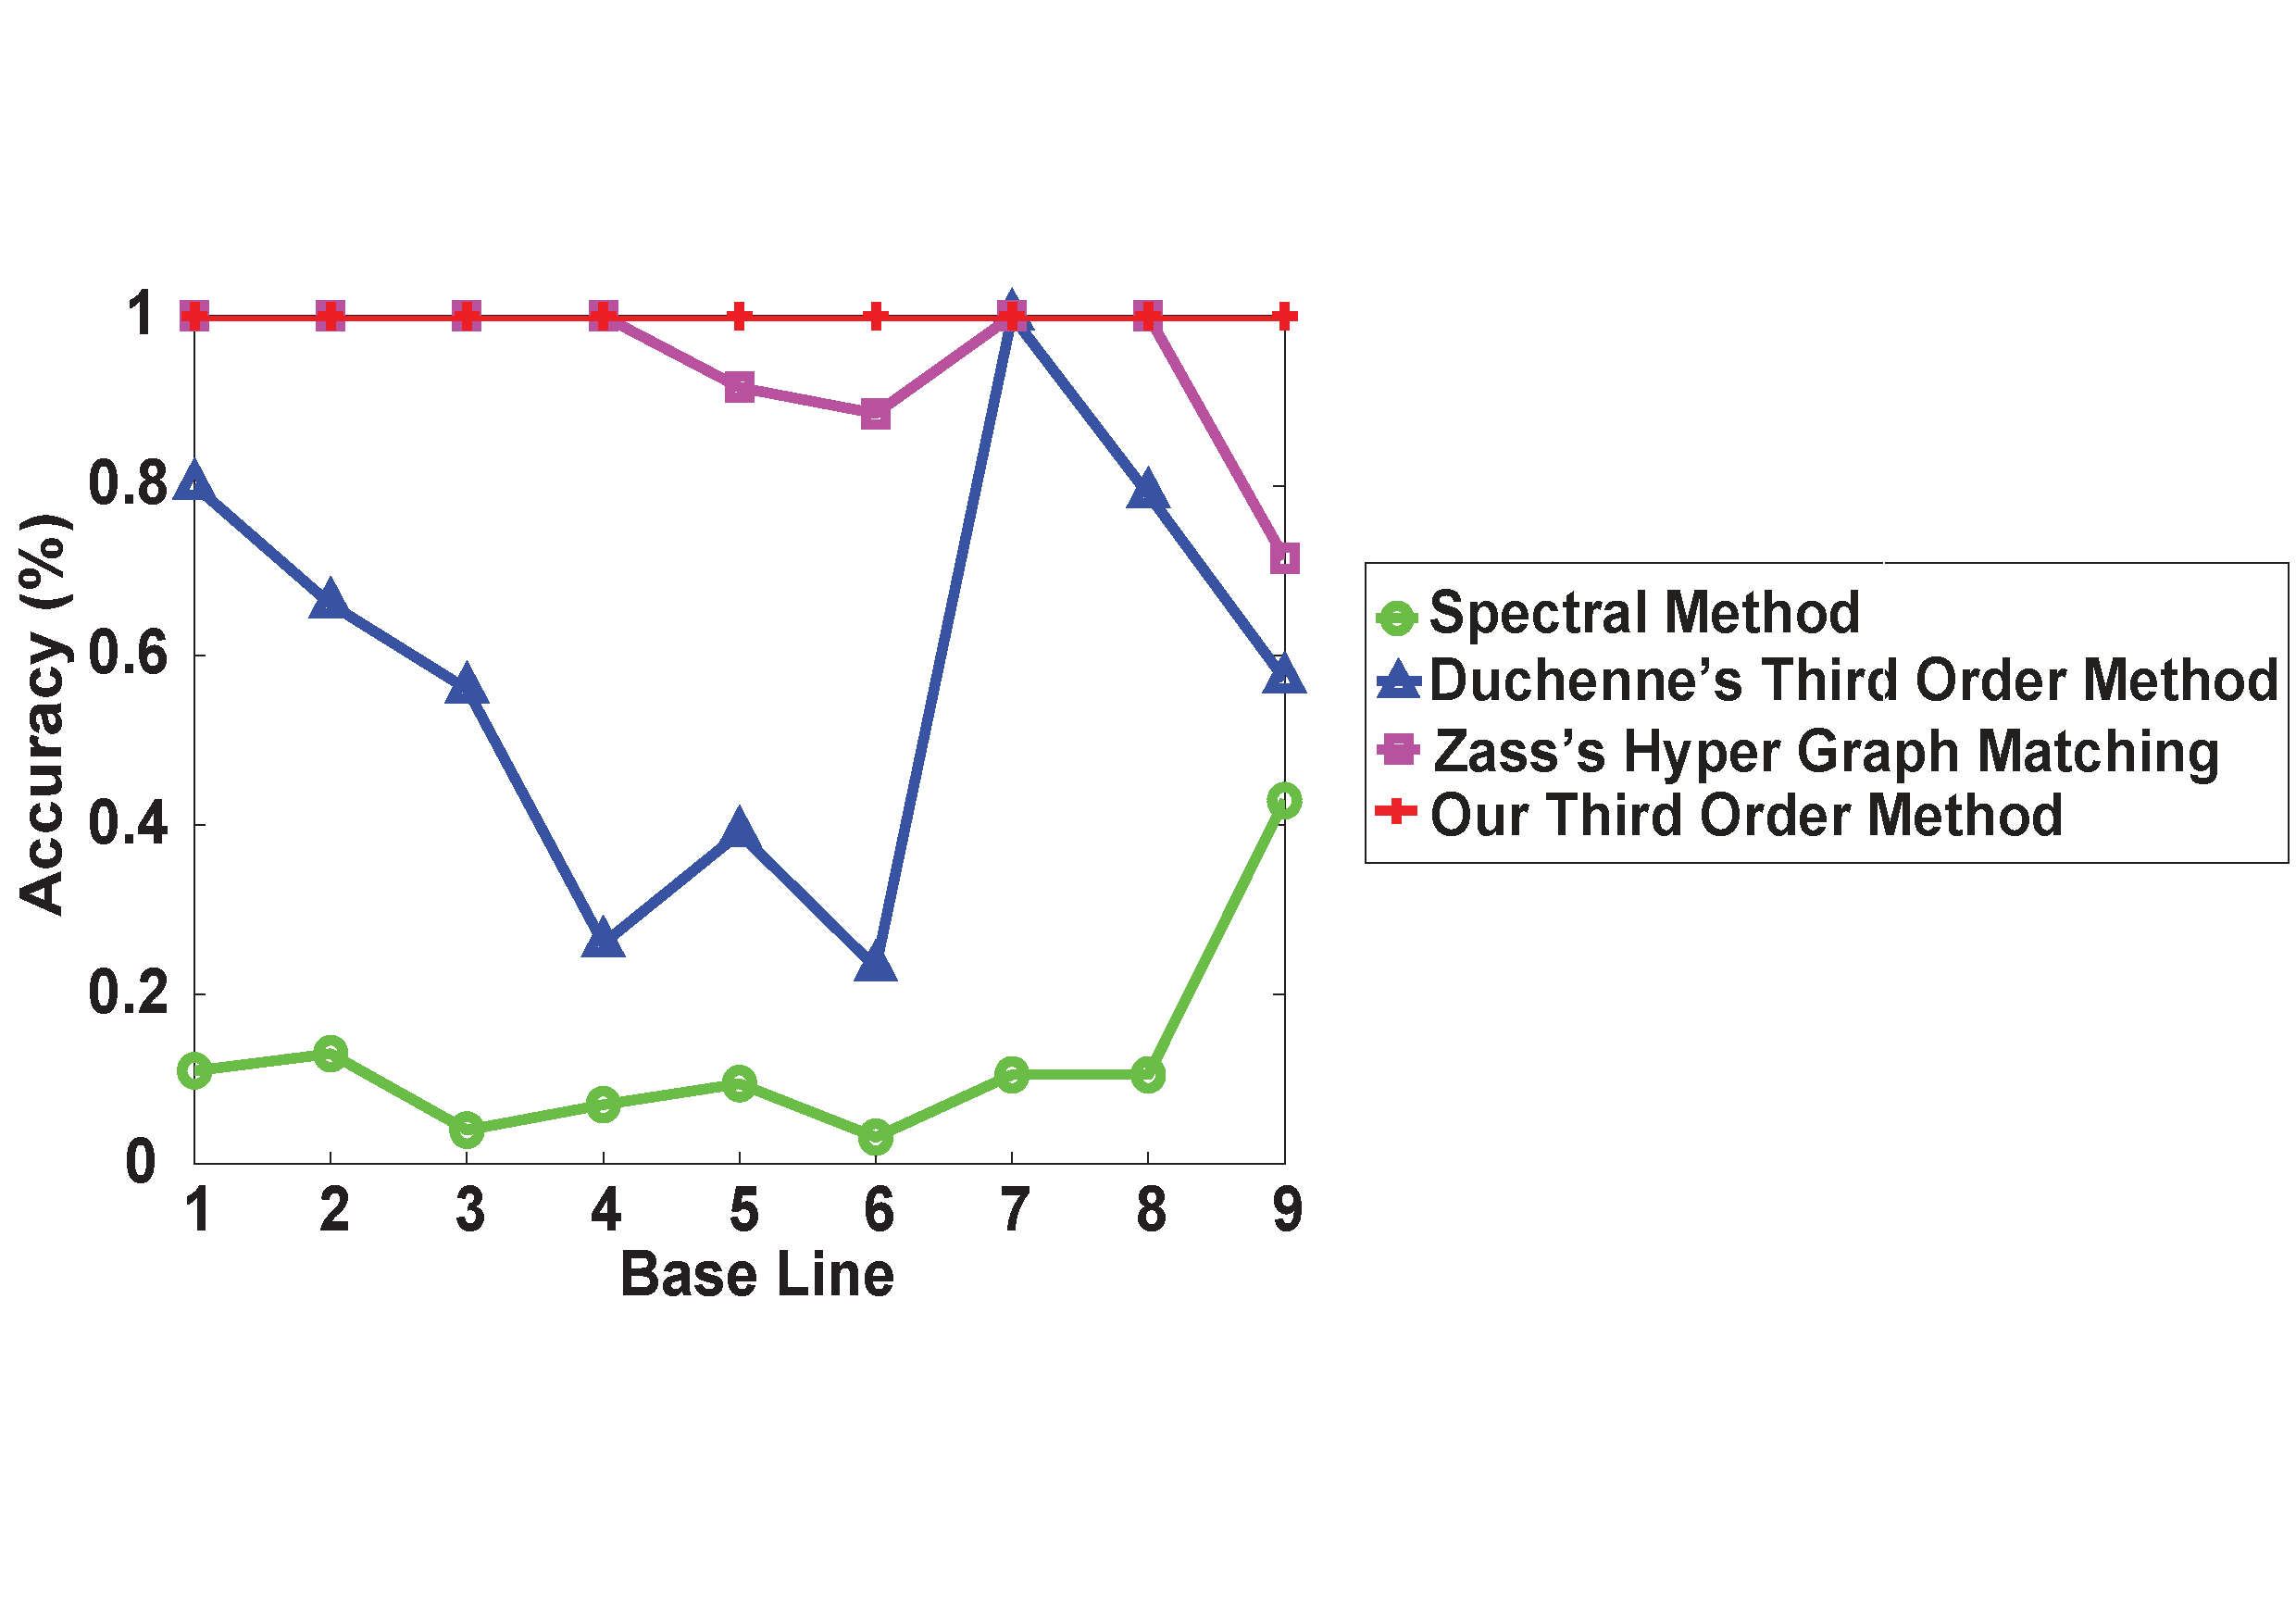
\includegraphics[width=130mm]{EXP3_ERROR_RATE_embedded2.pdf}%
     \caption{Accuracy as a function of base line.}
\label{fig:mini:projection_matchingaccuracy} %% label for entire figure
\end{figure*}%
%
\begin{figure*}[!t]
%%\hspace{-8ex}
\setlength{\abovecaptionskip}{0mm}
\setlength{\belowcaptionskip}{-2mm}
\centering
\setlength\subfigcapskip{-2mm}
\vspace{-4mm}
        % \hspace{-6ex}
        \begin{minipage}[b]{0.4\textwidth}
        \subfigure{
            \label{fig:subfig:housesmac}
            \centering
            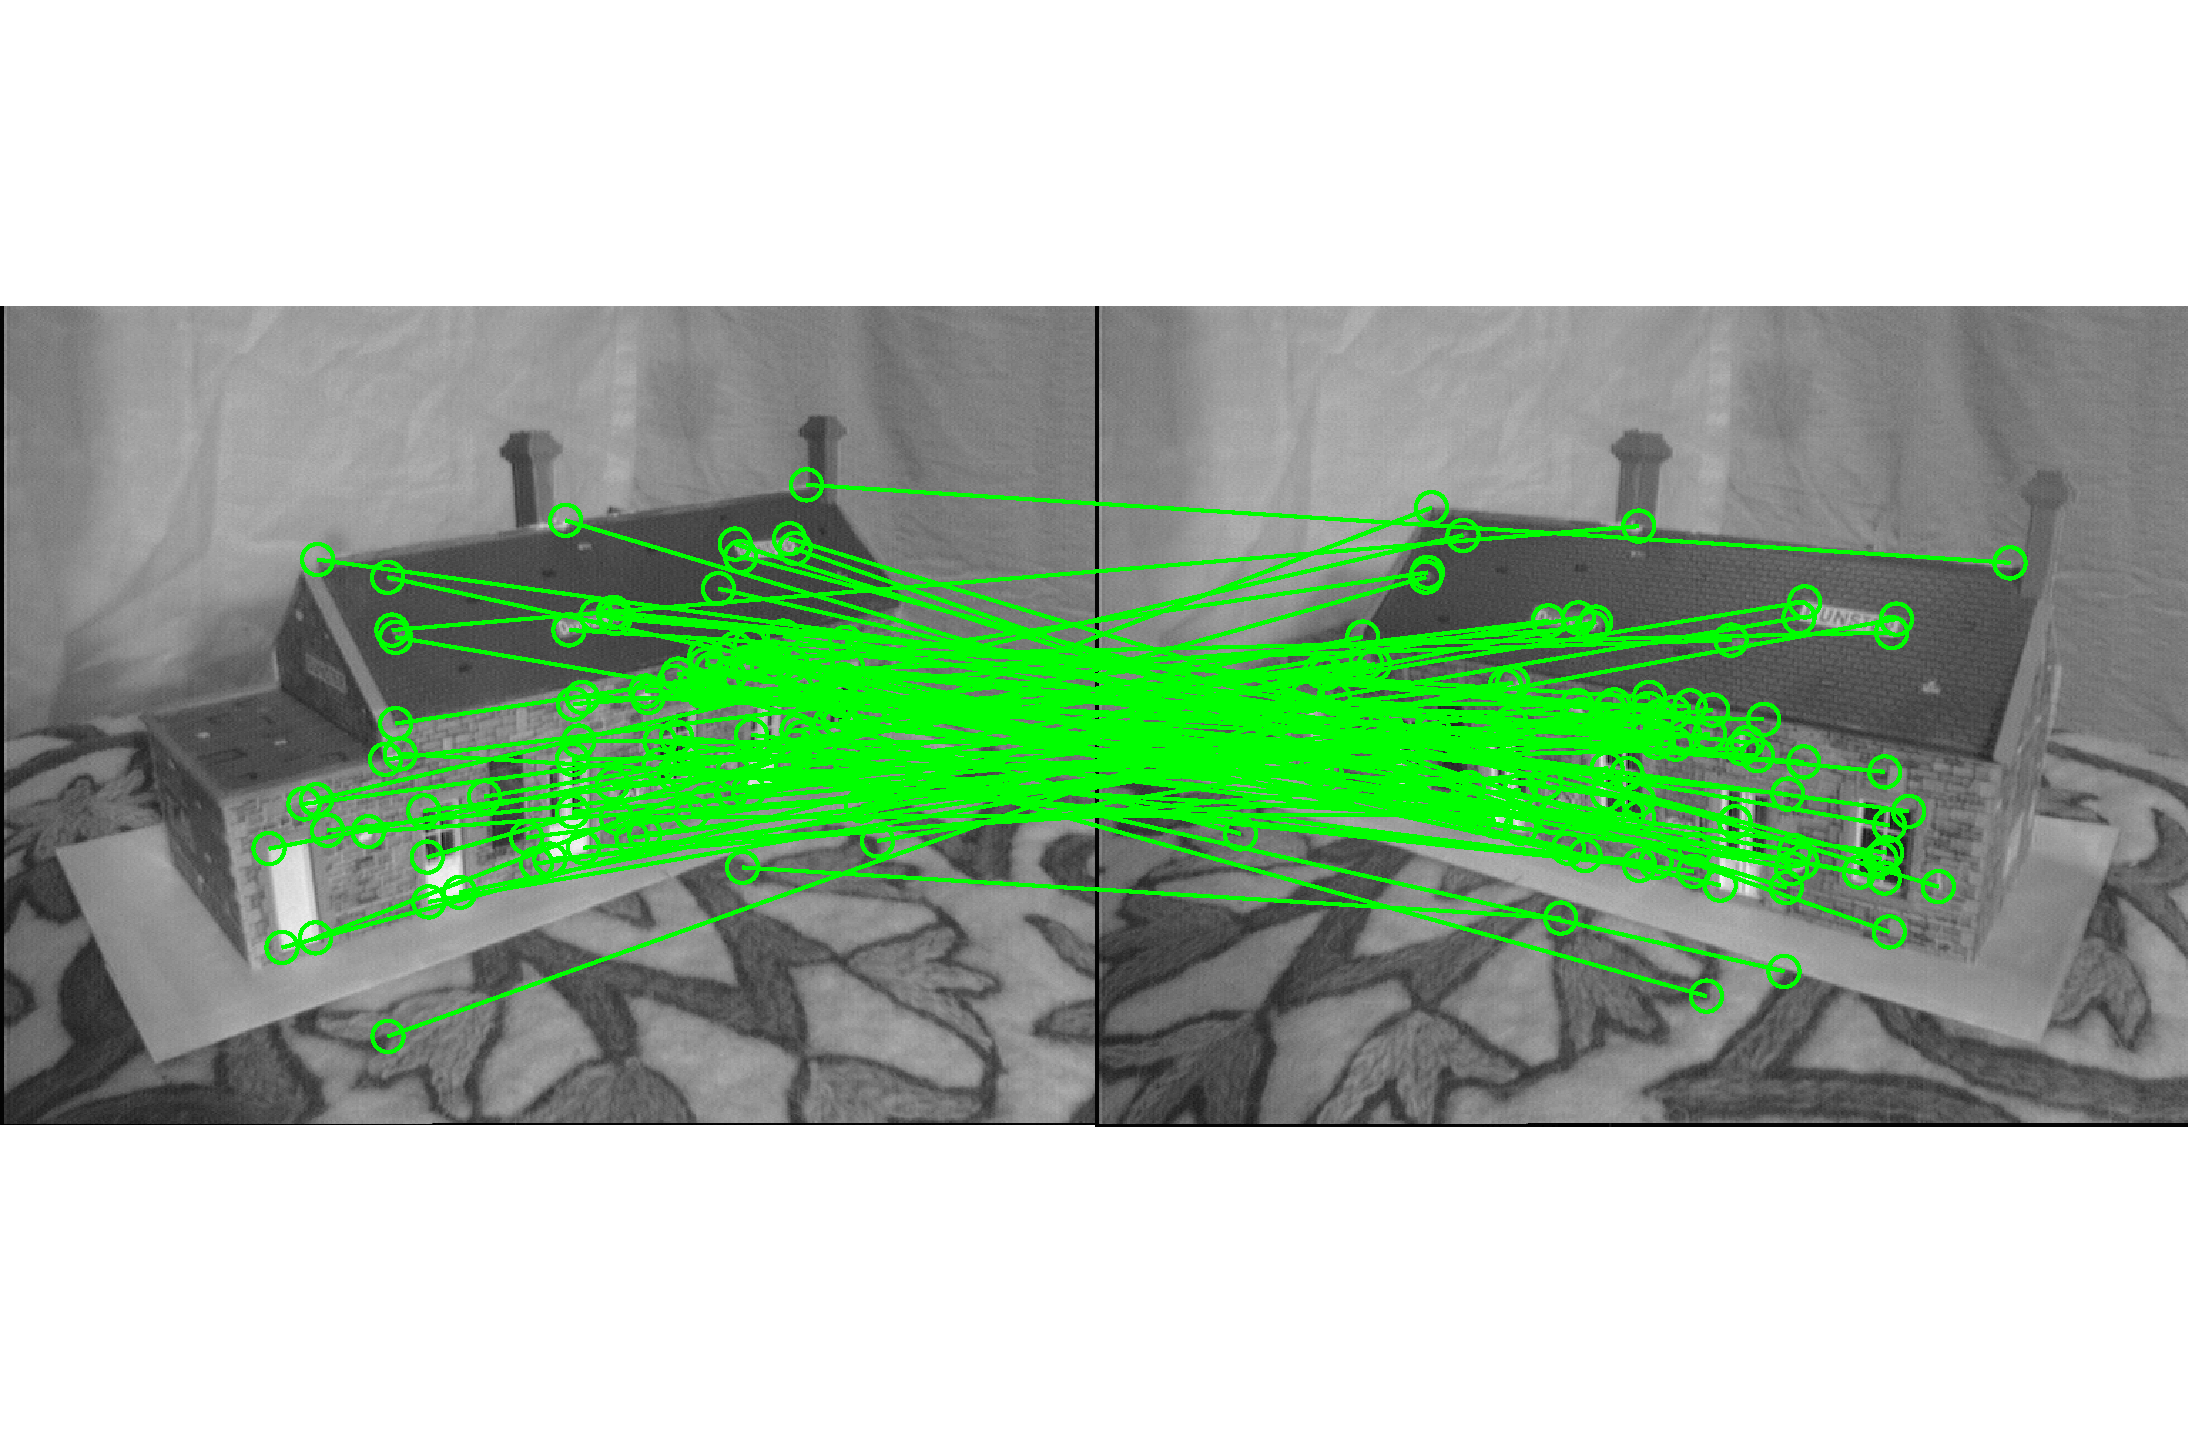
\includegraphics[width=60mm]{SMAC_EXP3_0-6.pdf}%
            }%
        \end{minipage}%
        %\hspace{10mm}%
        \addtocounter{subfigure}{-1}
        %%
        \begin{minipage}[b]{0.4\textwidth}
        \subfigure{
            \label{fig:subfig:housesmac2}
            \centering
            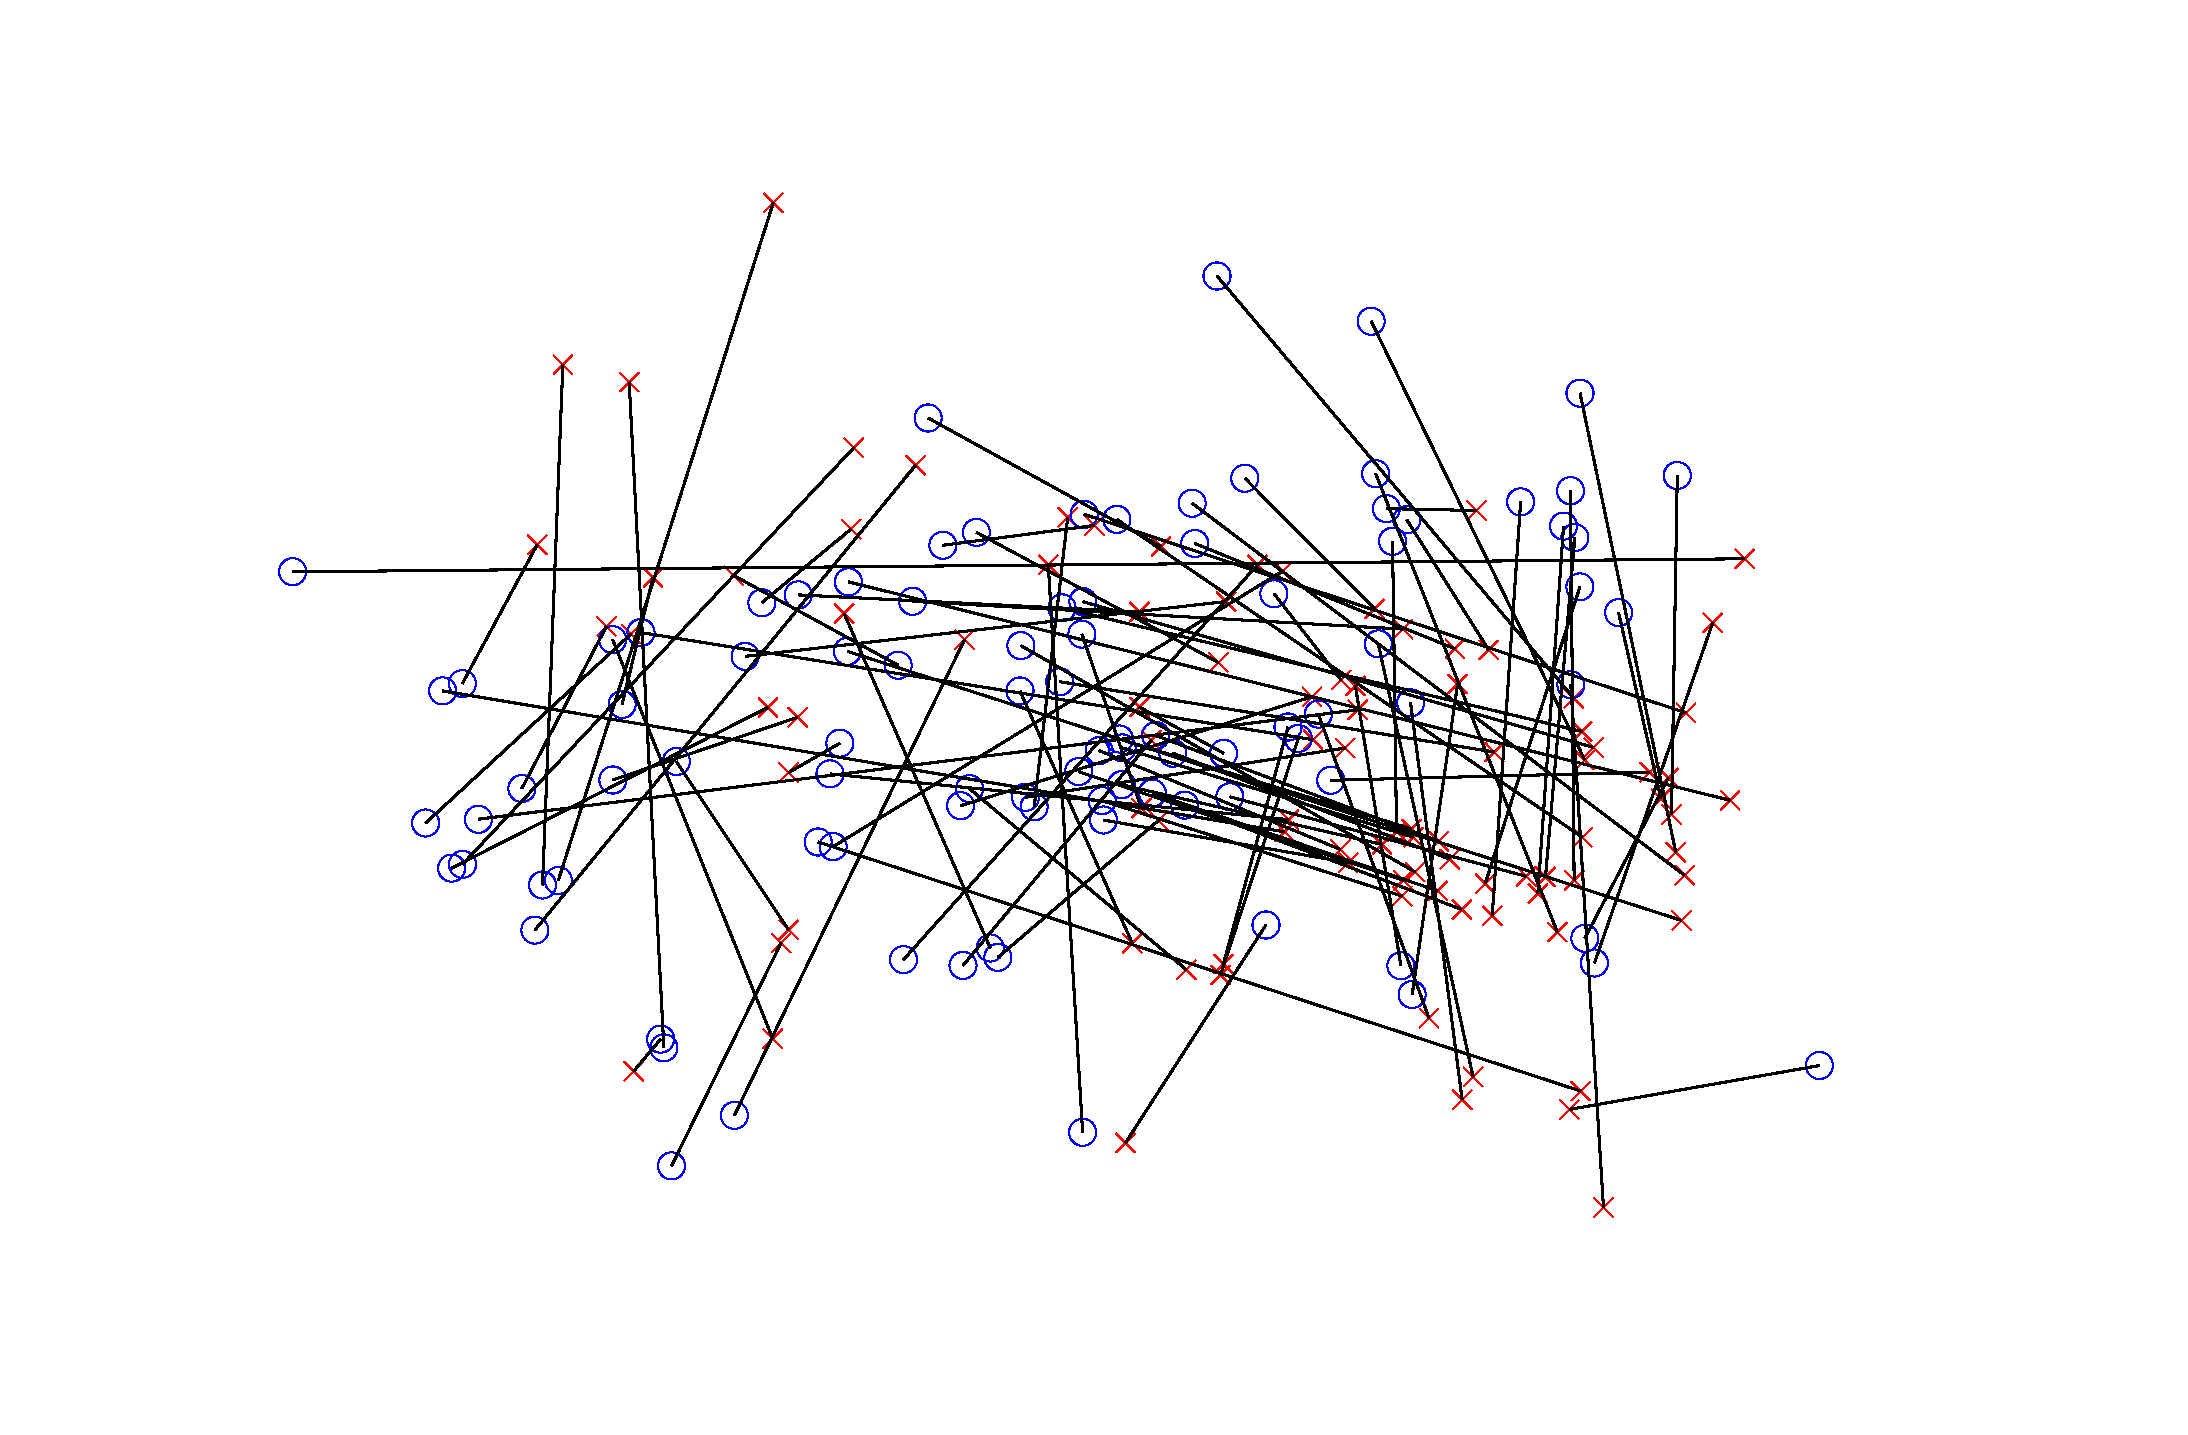
\includegraphics[width=50mm]{scatter_smac.pdf}%
            }%
        \end{minipage}\\%
        %\hspace{28mm}%
        \addtocounter{subfigure}{-1}
        %----------------------------
        \begin{minipage}[b]{0.4\textwidth}
        \subfigure{
            \label{fig:subfig:househyper}
            \centering
            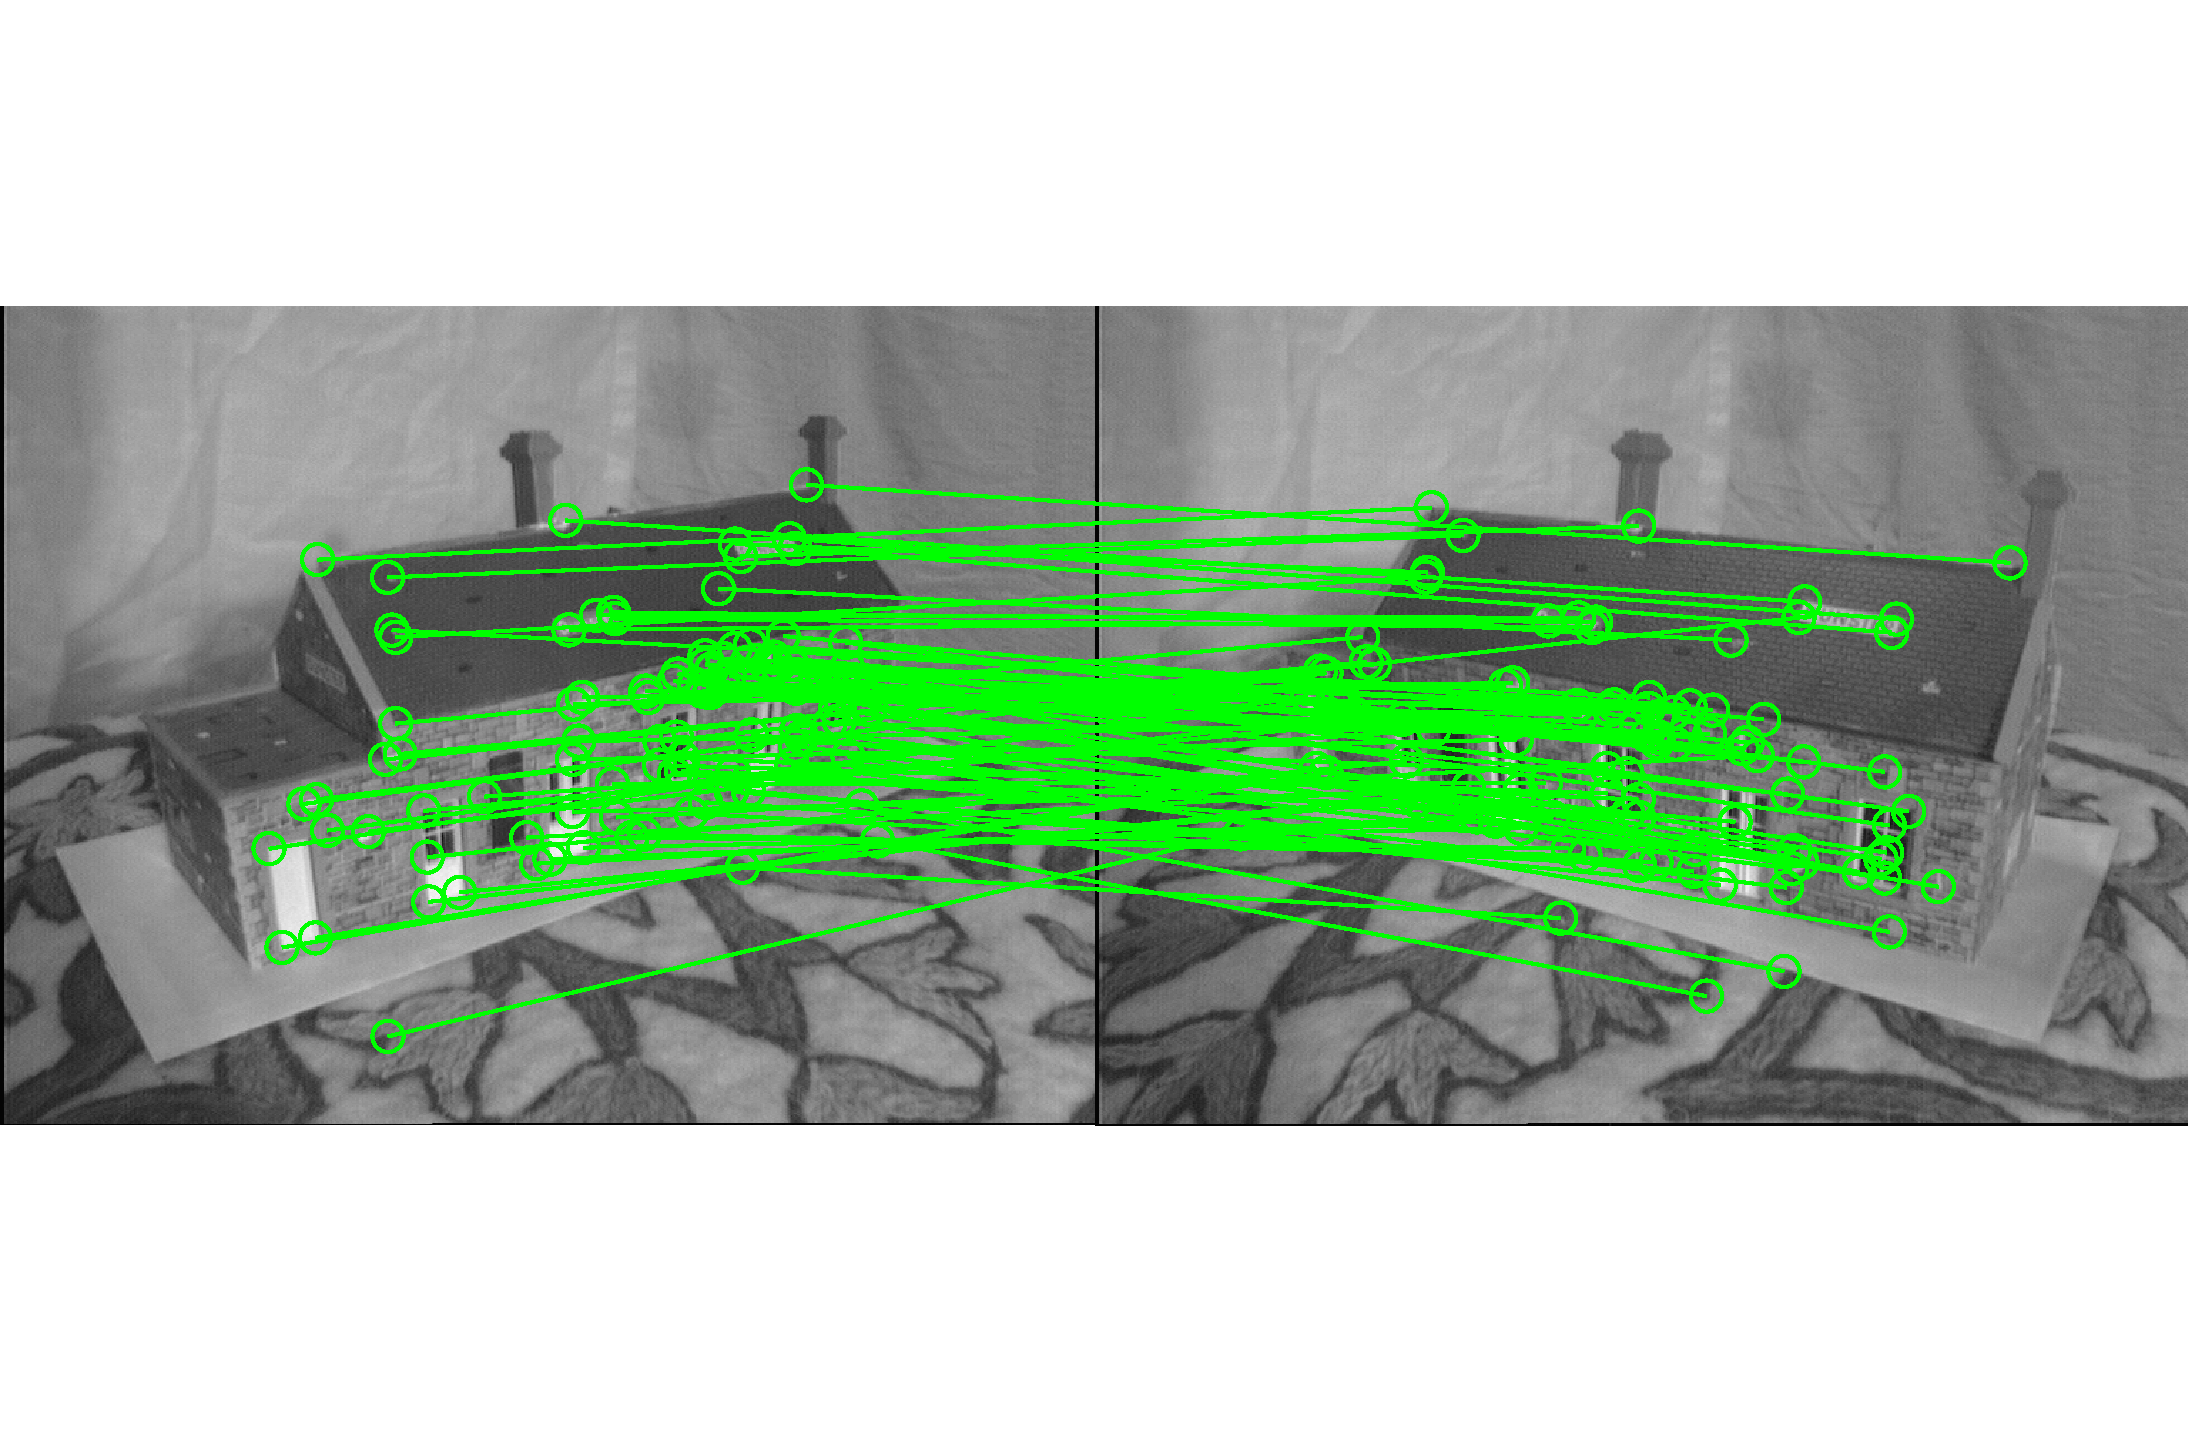
\includegraphics[width=60mm]{HYPER_EXP3_0-6.pdf}%
            }%
        \end{minipage}%
        %\hspace{28mm}%
        \addtocounter{subfigure}{-1}
         %%
        \begin{minipage}[b]{0.4\textwidth}
        \subfigure{
            \label{fig:subfig:househyper2}
            \centering
            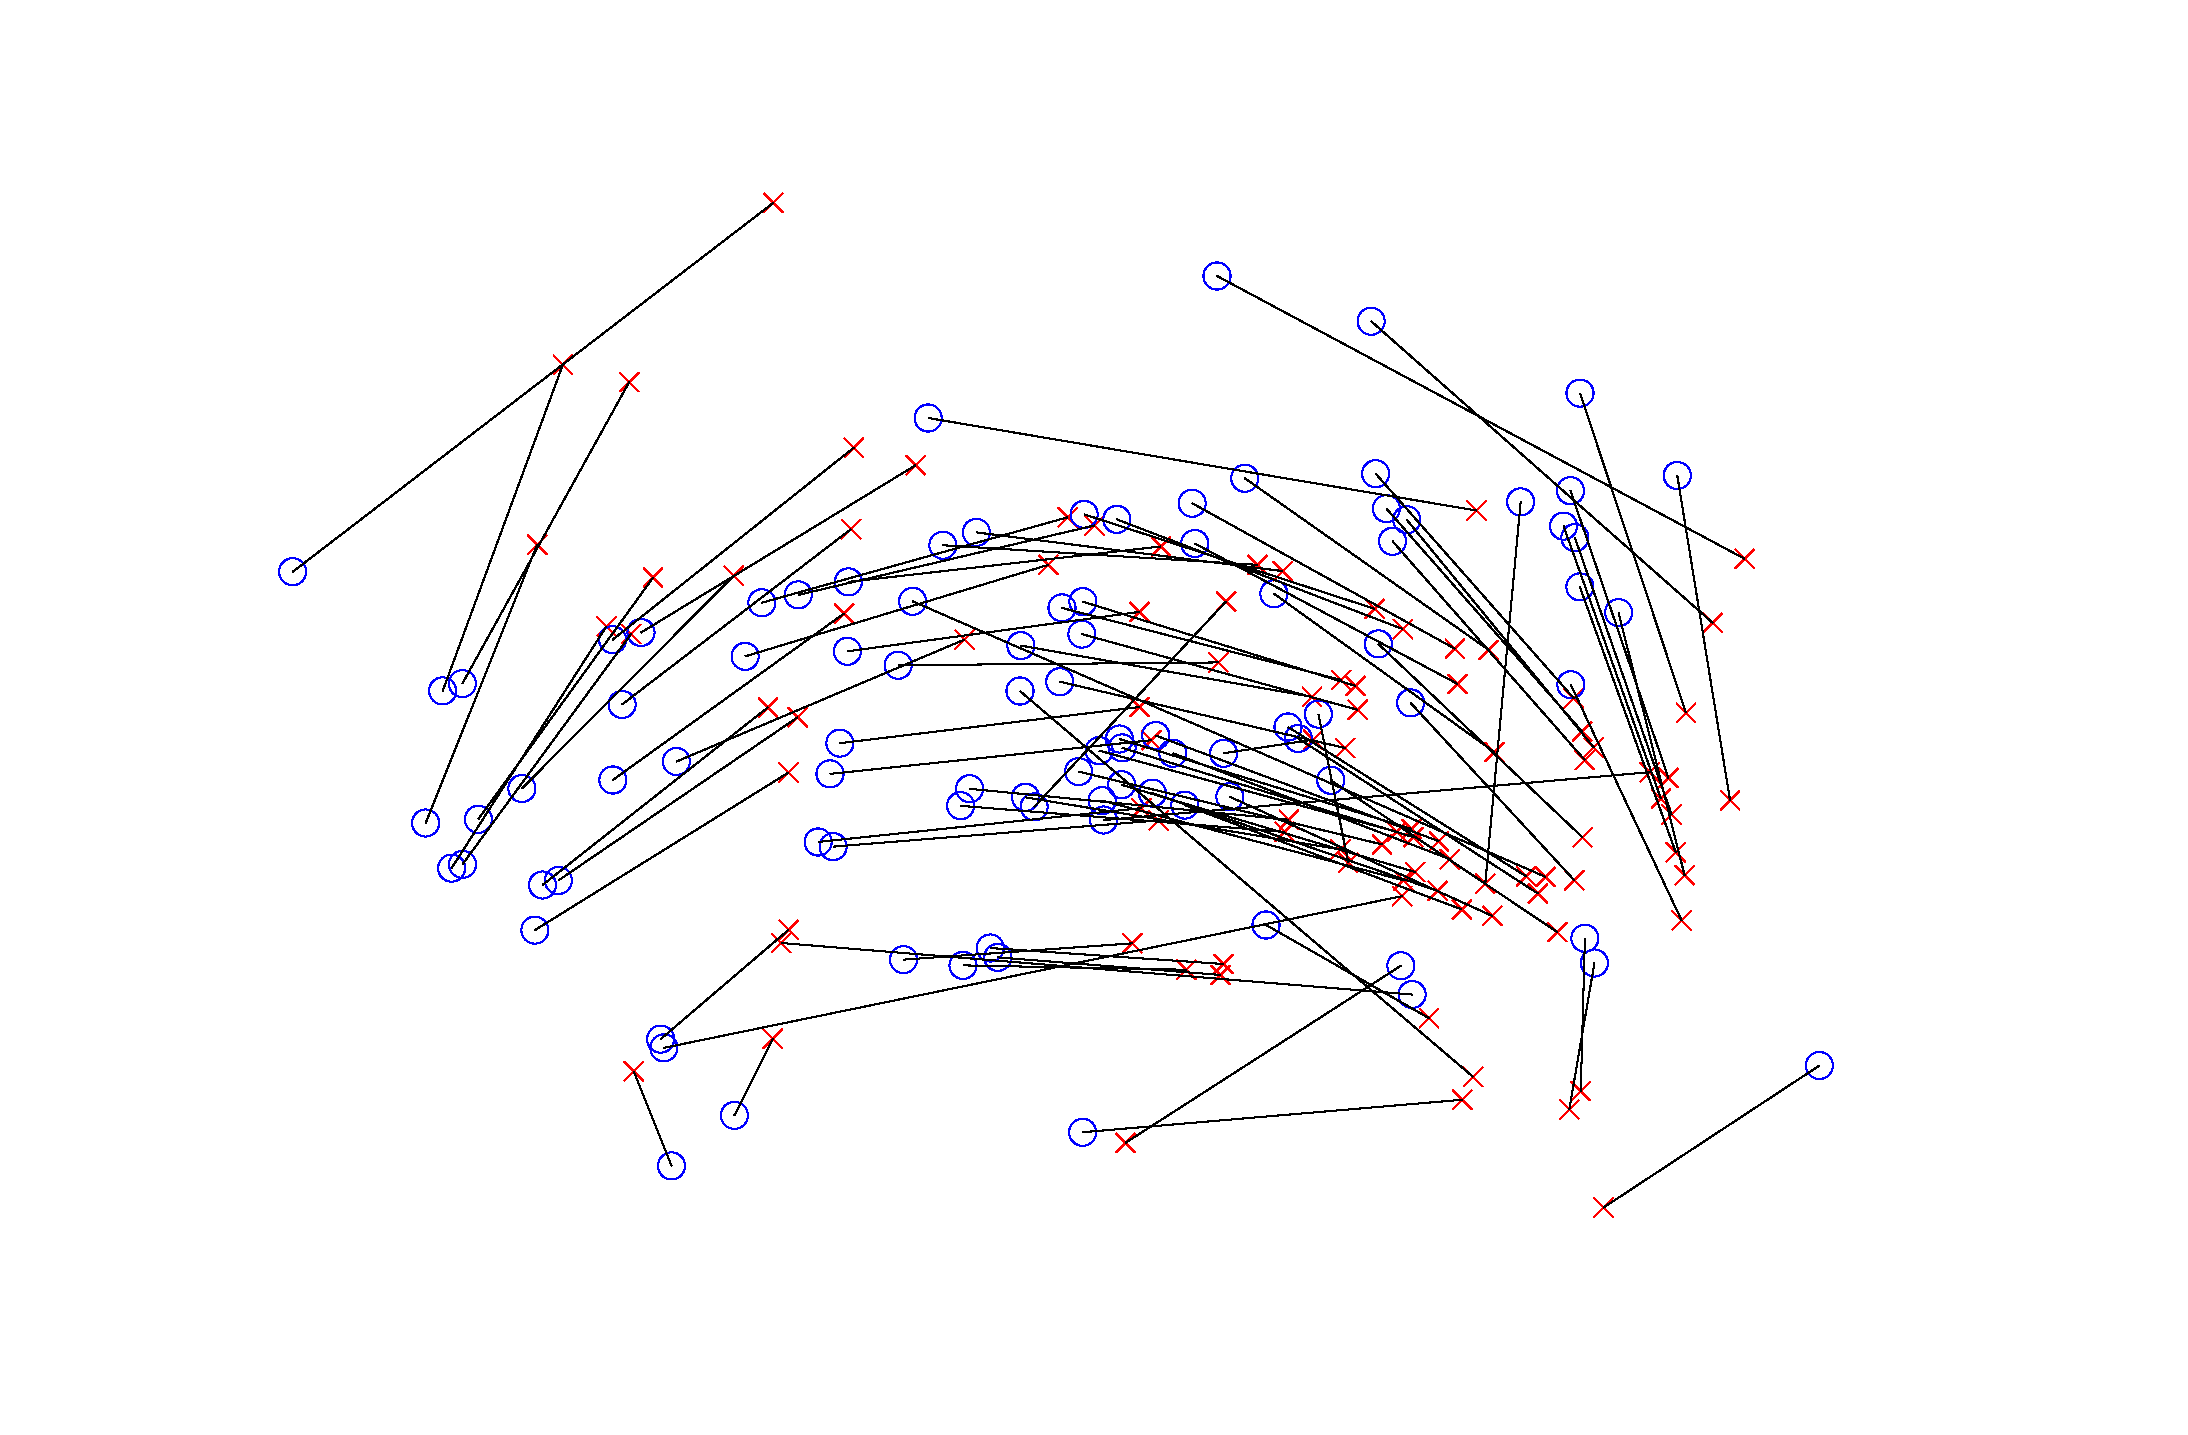
\includegraphics[width=50mm]{scatter_hyper.pdf}%
            }%
        \end{minipage}\\%
        %\hspace{28mm}%
        \addtocounter{subfigure}{-1}
        %----------------------------
        %\hspace{-6ex}
        \begin{minipage}[b]{0.4\textwidth}
        \subfigure{
            \label{fig:subfig:housedemo}
            \centering
            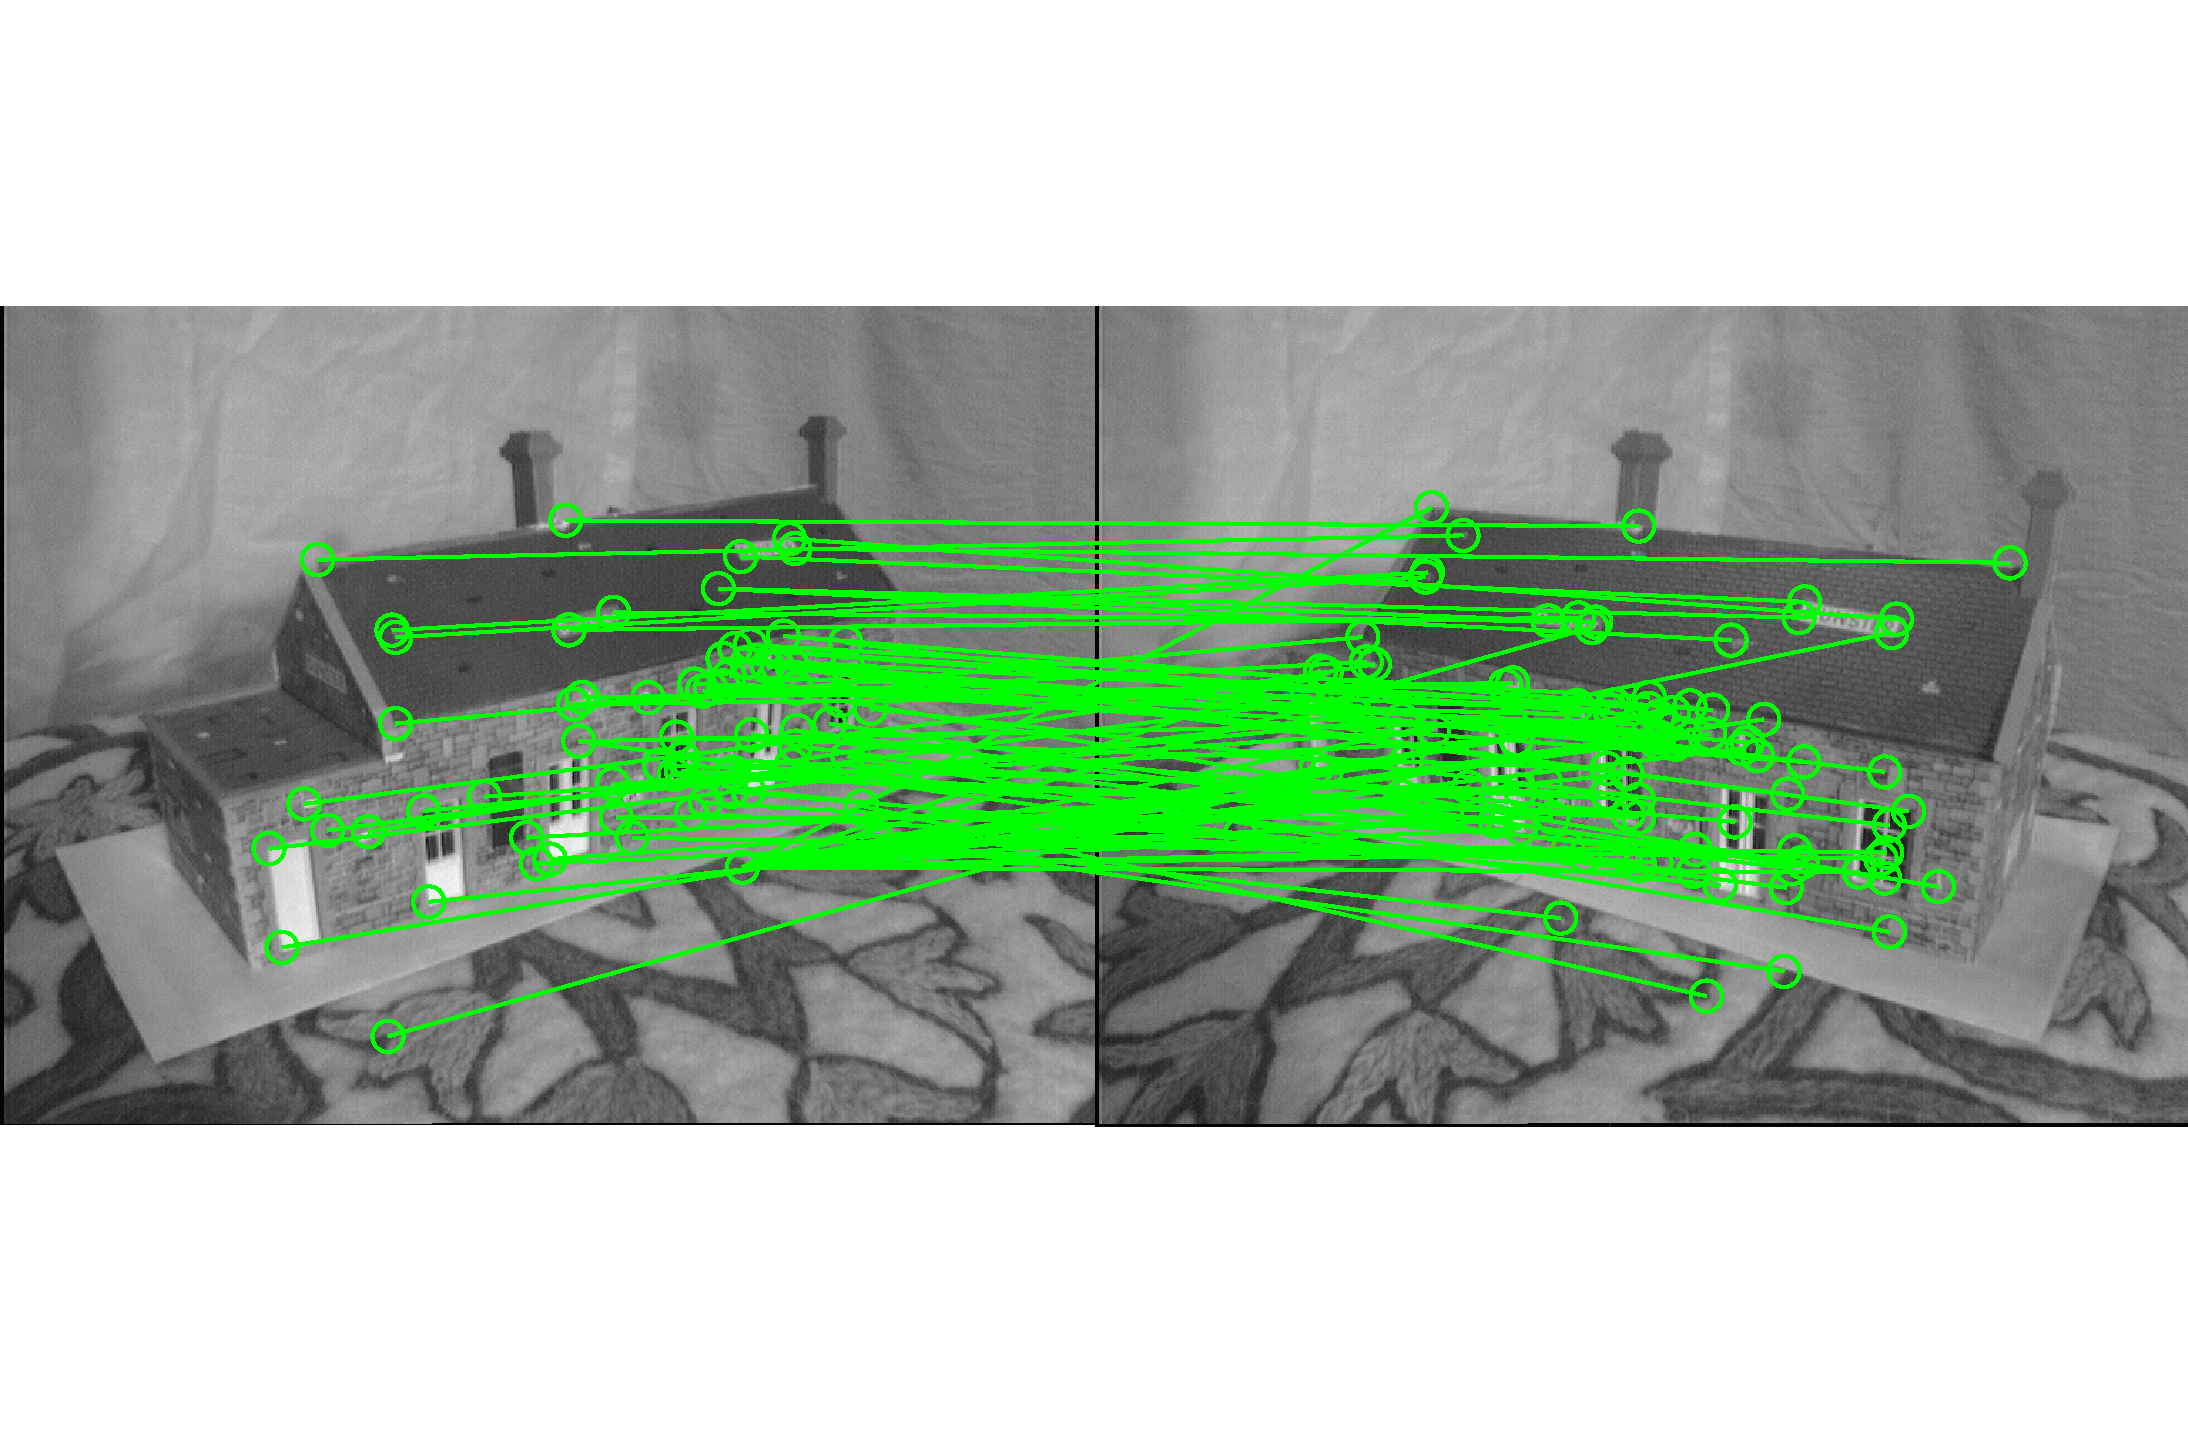
\includegraphics[width=60mm]{DEMO_EXP3_0-6.pdf}%
            }%
        \end{minipage}%
        %\hspace{10mm}%
        \addtocounter{subfigure}{-1}
         %%
        \begin{minipage}[b]{0.4\textwidth}
        \subfigure{
            \label{fig:subfig:housedemo2}
            \centering
            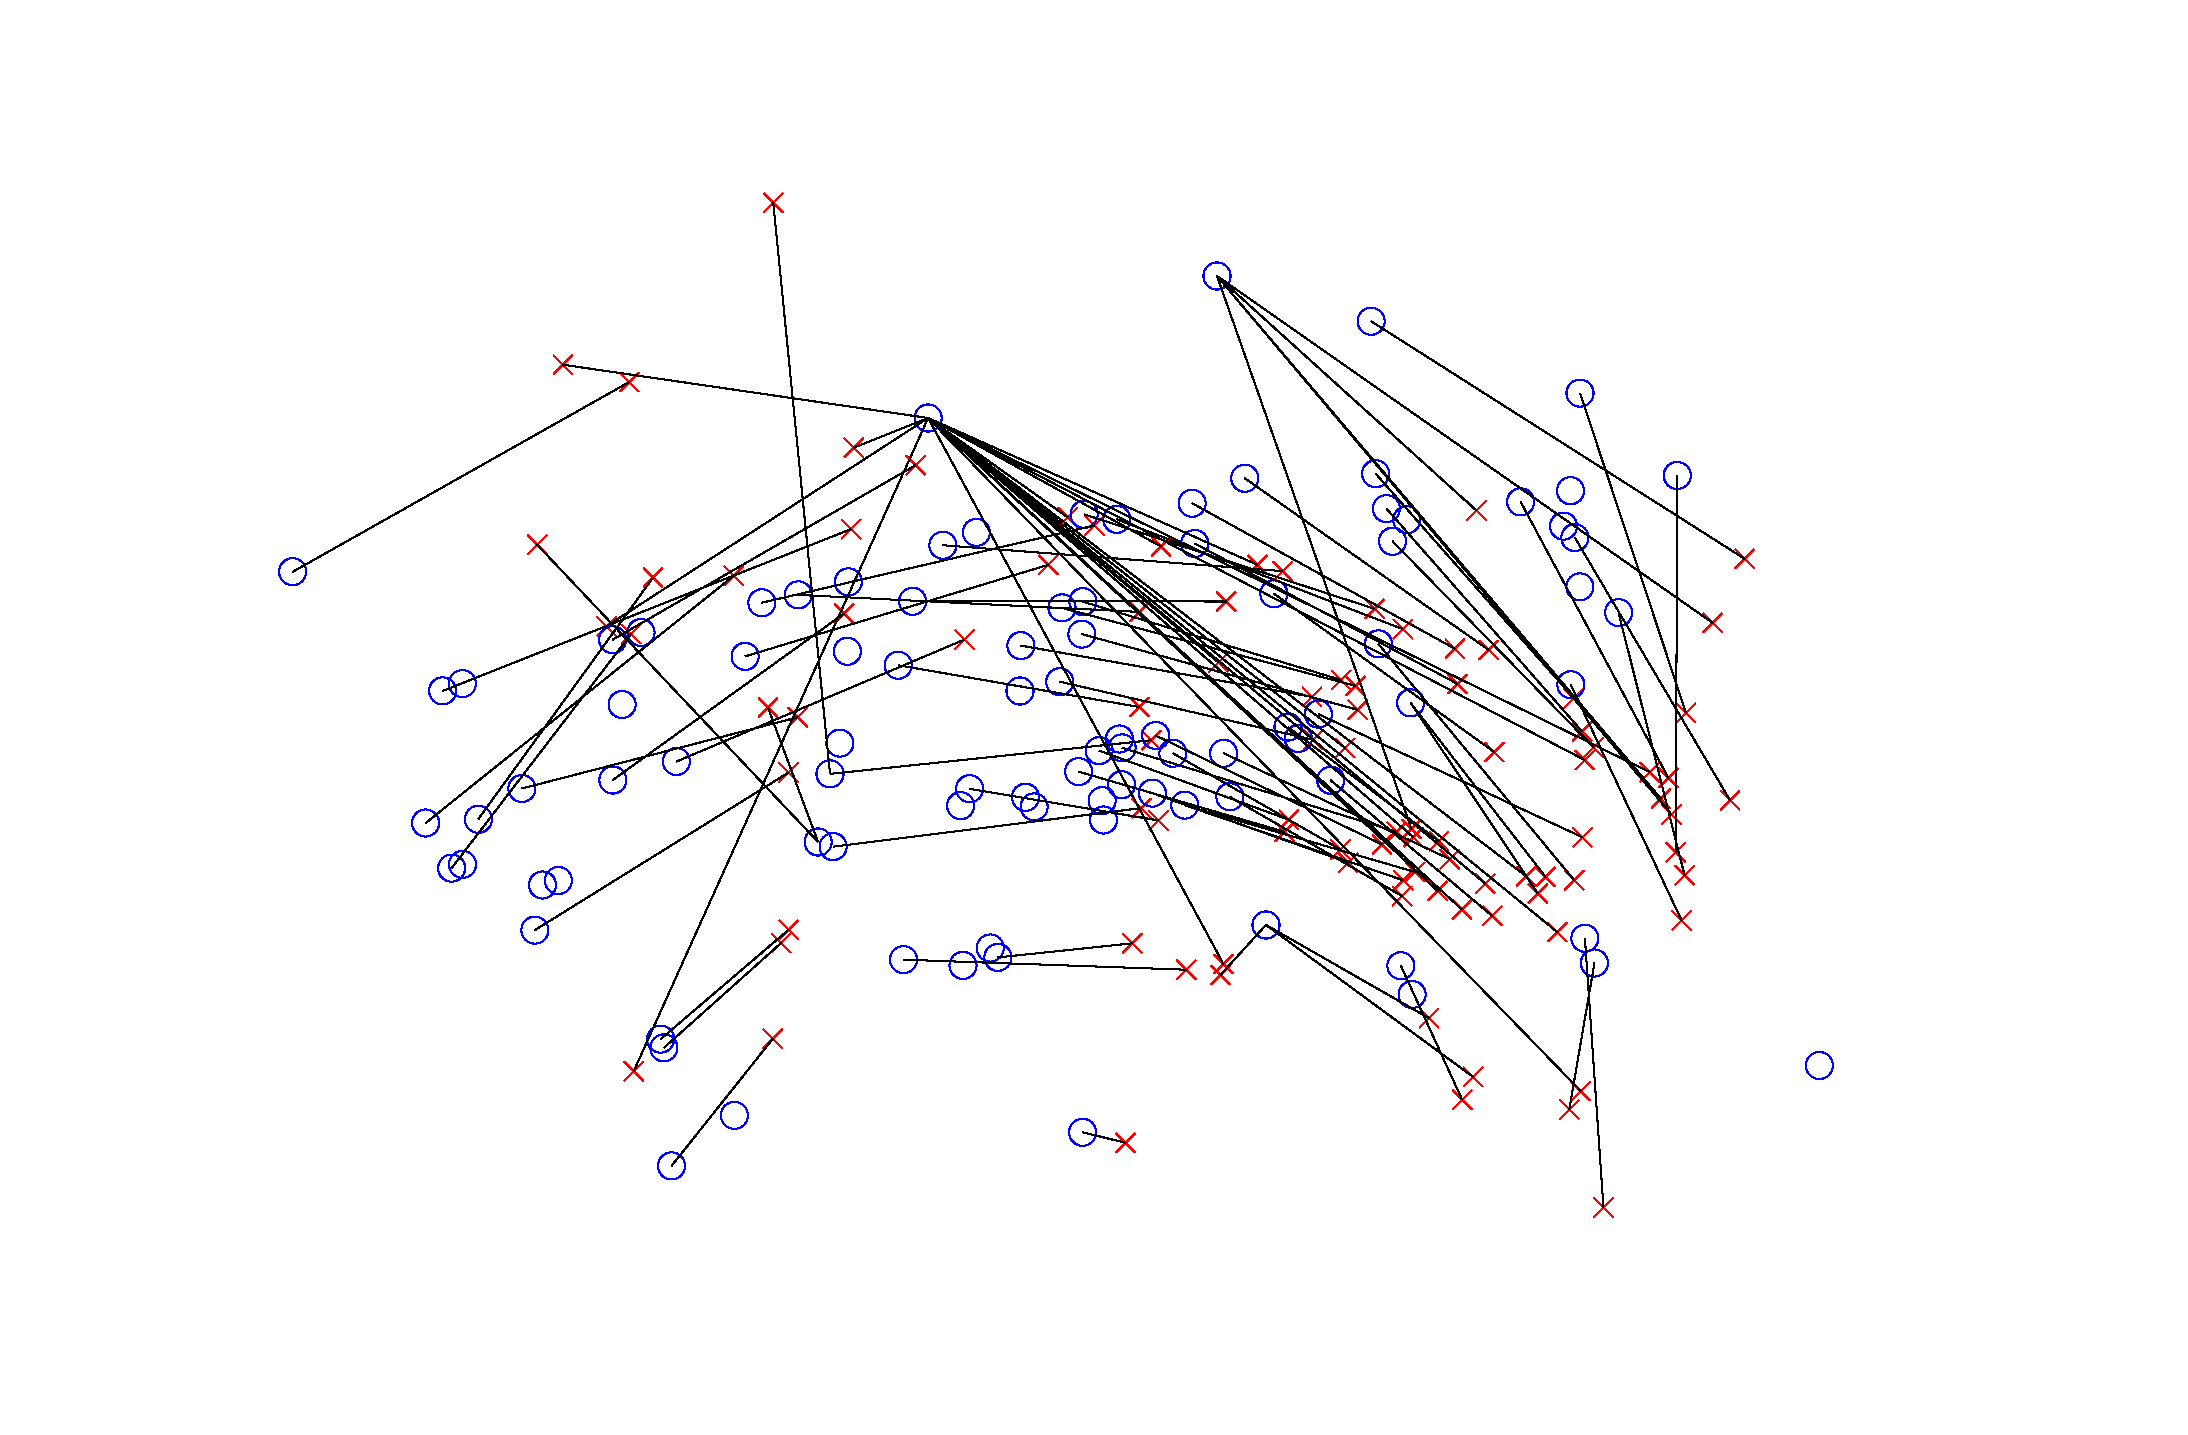
\includegraphics[width=50mm]{scatter_demo.pdf}%
            }%
        \end{minipage}\\%
        %\hspace{28mm}%
        \addtocounter{subfigure}{-1}
        %----------------------------
        \begin{minipage}[b]{0.4\textwidth}
        \subfigure[]{
            \label{fig:subfig:houseour}
            \centering
            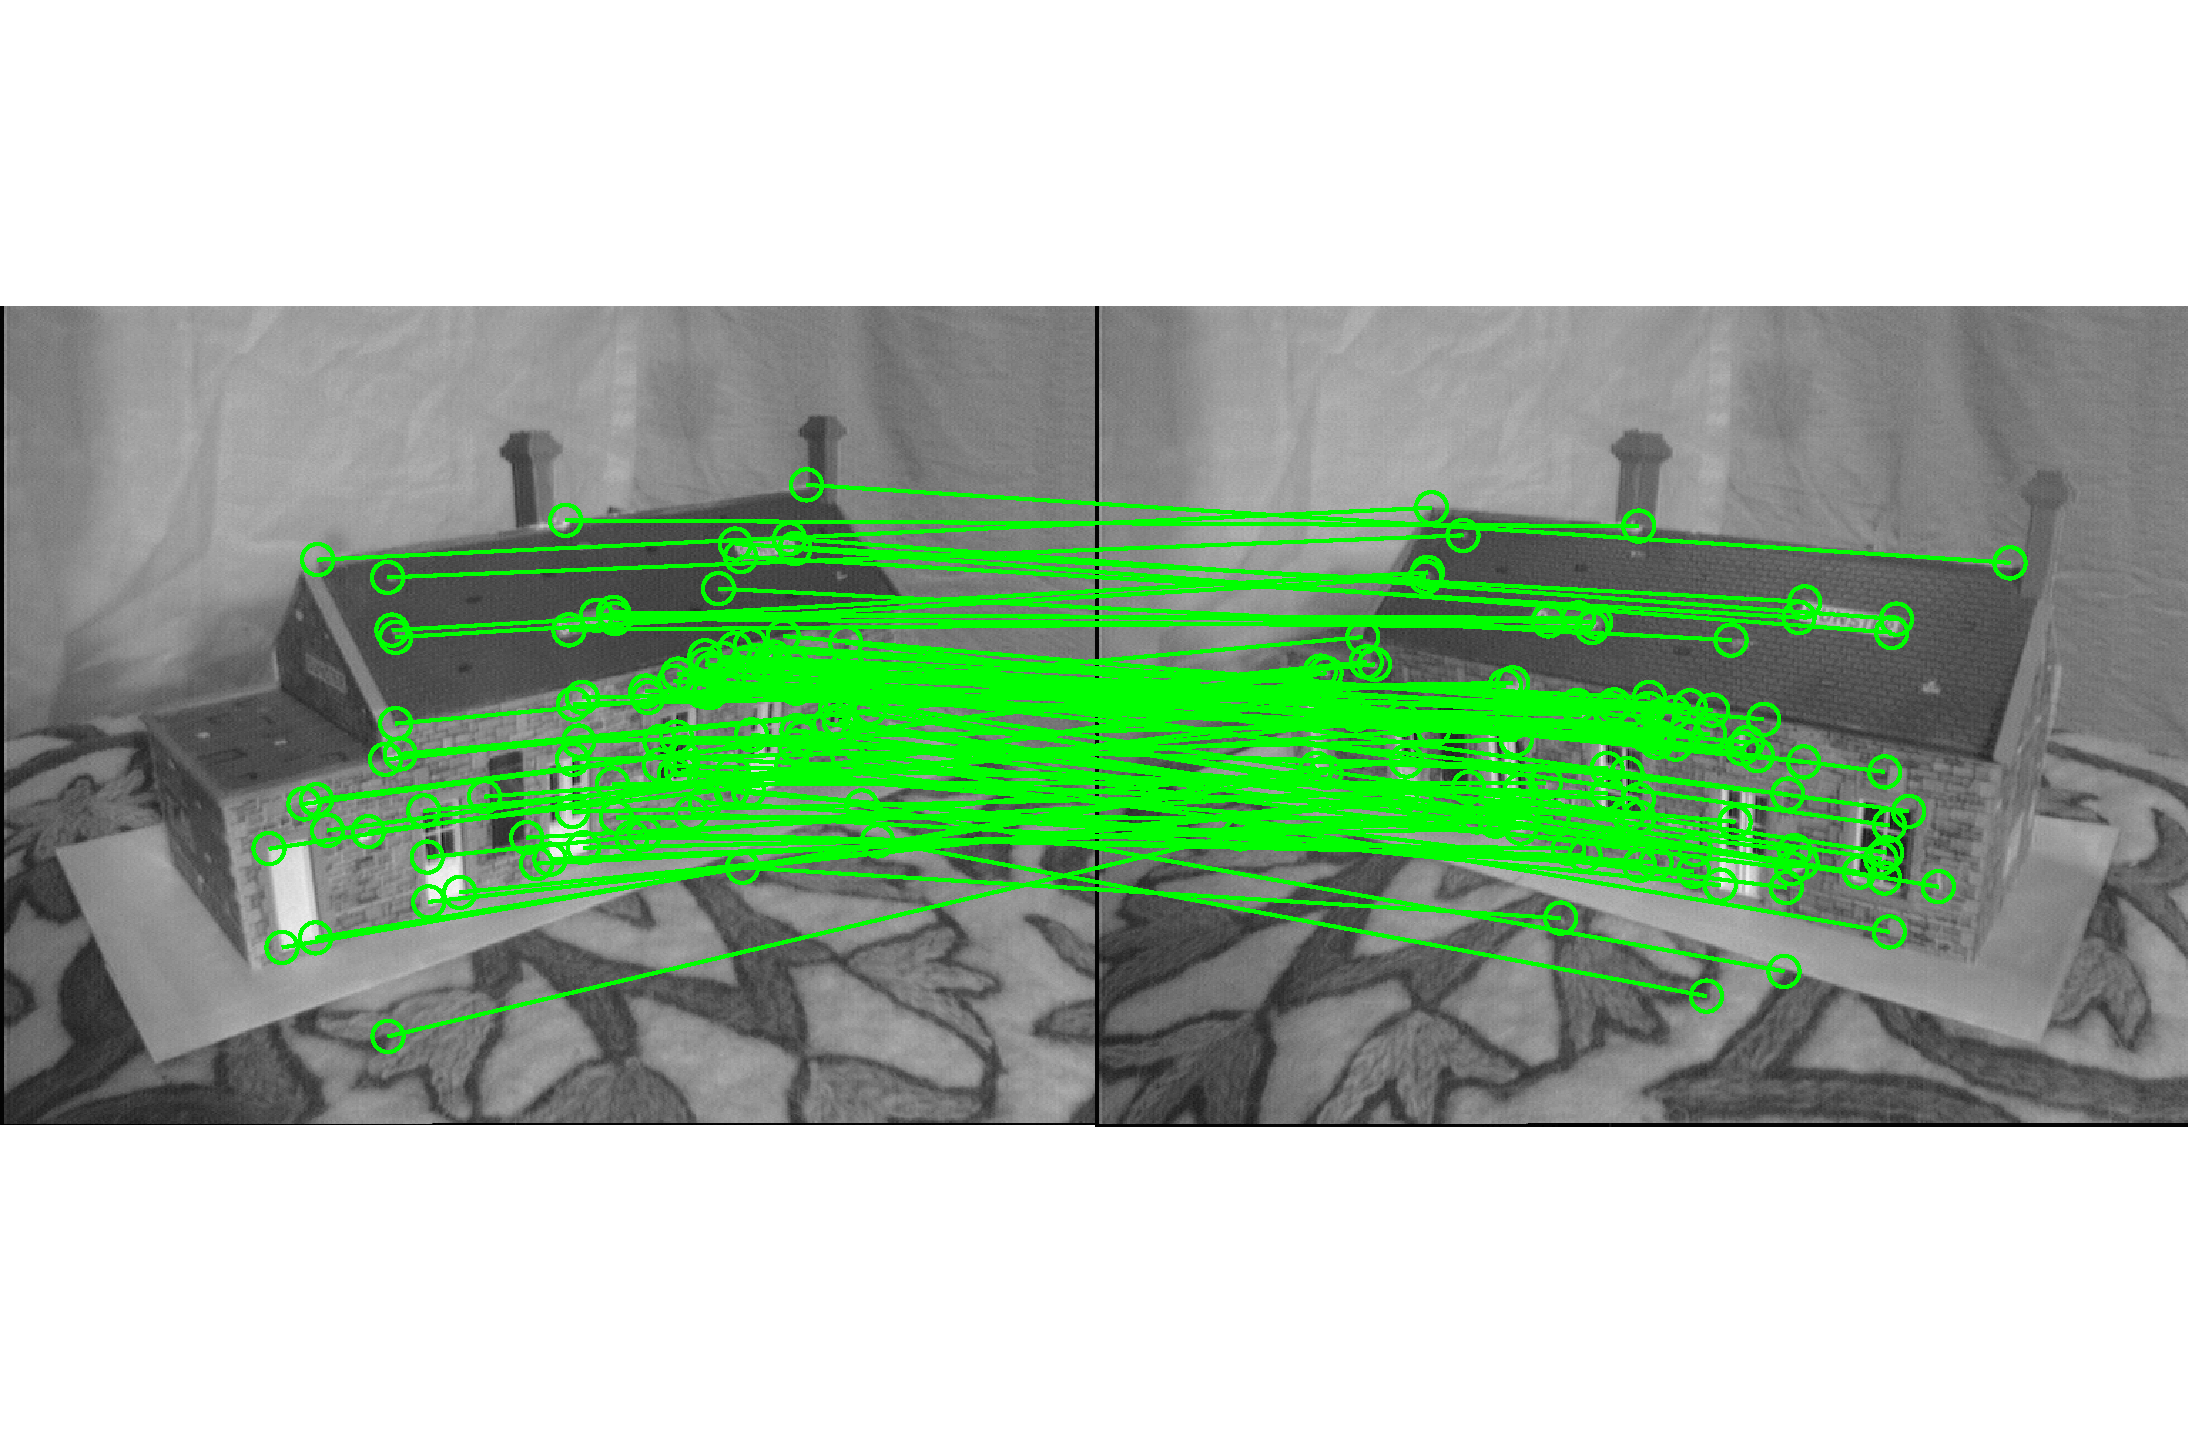
\includegraphics[width=60mm]{OUR_EXP3_0-6.pdf}%
            }%
        \end{minipage}%
        %\hspace{24mm}%
        %\addtocounter{subfigure}{-1}
        %%
        \begin{minipage}[b]{0.4\textwidth}
        \subfigure[]{
            \label{fig:subfig:houseour2}
            \centering
            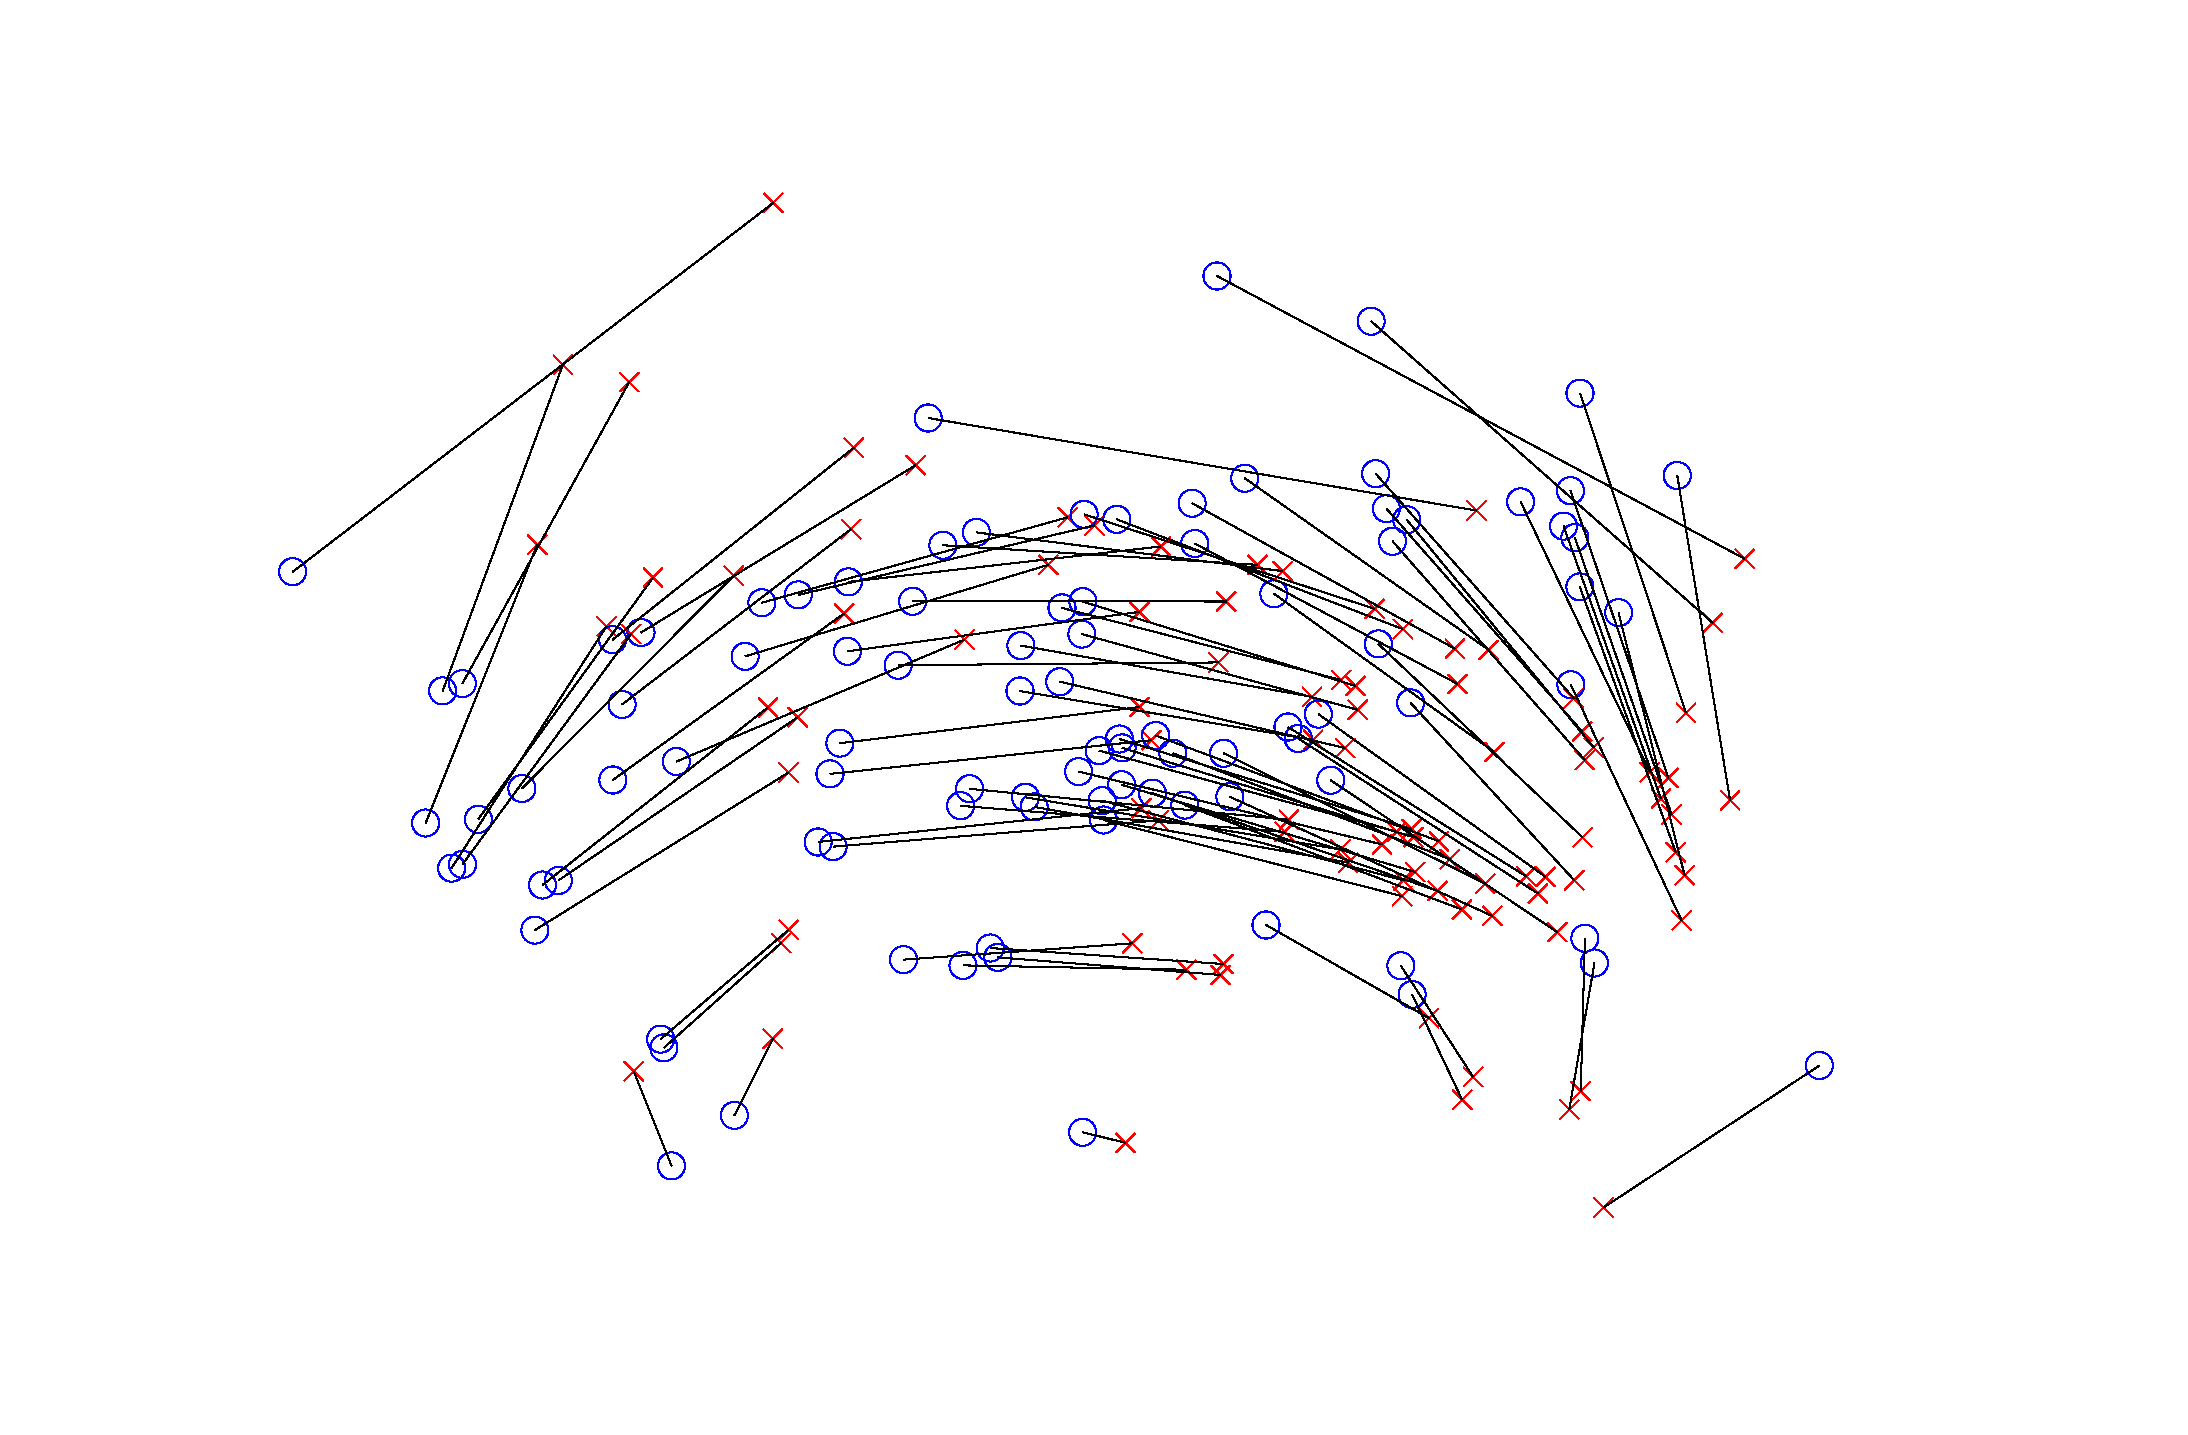
\includegraphics[width=50mm]{scatter_our.pdf}%
            }%
        \end{minipage}%
        %\hspace{28mm}%
        %\addtocounter{subfigure}{-1}
        \caption{Matching images 0 and 6 for the \texttt{house} data. Top to bottom: results of the spectral method~\cite{Cour06}, the hyper graph matching method~\cite{Zass08}, the tensor based method~\cite{Duchenne_etal09} and our method. Left: matches. Right: scatter diagrams of matching results; red $\textcolor{red}{\times}$ and blue $\textcolor{blue}{\circ}$ represent two graphs respectively.}
\label{fig:mini:projection_matchingimages} %% label for entire figure
\end{figure*}%

The larger the baseline separating the images, the larger the relative deformation, and hence the more difficult to match. From Fig.~\ref{fig:mini:projection_matchingaccuracy}, it is clear that our method is remains stable as the baseline increases, and is the most accurate method. Even though there are only seven Harris corners in each frame, it is still difficult to match because of the large viewpoint differential. The average number of sampling feature tuples for all nine baseline matches are $13161$, $643305$ and $26322$ for our method, the method in~\cite{Duchenne_etal09} and  the method in~\cite{Zass08} respectively.
